\documentclass[a4paper, 12pt, openany, oneside]{memoir}

\usepackage{multirow}
\usepackage{tabulary}

\usepackage[sort&compress,numbers]{natbib}

%\usepackage{doi}%<----------



\usepackage{hyperref}
\usepackage{memhfixc}
\hypersetup{final}
\usepackage{color}
\usepackage{graphicx}
\usepackage{nomencl}
\usepackage{paralist}
\usepackage{feynmp}
%\usepackage{feynmp-auto}
\newsubfloat{figure}
%\usepackage{caption}
%\usepackage{subcaption}
\usepackage{amsmath}
\usepackage{amssymb}
%\usepackage[pdf]{pstricks}
\usepackage{epstopdf}
\usepackage{verbatim}
\usepackage{xspace}


\setlrmarginsandblock{2in}{1in}{*}
\setulmarginsandblock{1.25in}{1.25in}{*}
\checkandfixthelayout

\makeheadrule{headings}{\textwidth}{0.3pt}

%MAY NEED TO SPECIFY THE CAPTION FONTS!!!
\changecaptionwidth
\captionwidth{0.9\textwidth}
\captionnamefont{\small}
\captiontitlefont{\small}


\DeclareGraphicsRule{*}{mps}{*}{}
%\DeclareGraphicsRule{.eps}{pdf}{-eps-converted-to.pdf}{}

\setsecnumdepth{subsection}

\newcommand{\note}[1]{\textcolor{red}{\textbf{#1}}}

\newcommand{\todo}[1]{\textcolor{blue}{\textit{#1}}}


\newcommand{\etal}{et al.\ }
\newcommand{\LCDM}{$\Lambda$CDM}
\newcommand{\dbd}[2]{\frac{\mathrm{d}#1}{\mathrm{d}#2}}
\newcommand{\GeV}{\textrm{ GeV}}
\newcommand{\cmsq}{\textrm{ cm}^2}
\newcommand{\kms}{\,\textrm{km s}^{-1}}
\newcommand{\qhat}{\hat{\textbf{q}}}
\newcommand{\vhat}{\hat{\textbf{v}}}
\newcommand{\boldtheta}{\boldsymbol\theta}
\newcommand{\boldpsi}{\boldsymbol\psi}
\newcommand{\boldphi}{\boldsymbol\phi}
\newcommand{\PLF}{polynomial $\ln f(v)$\xspace}

\newcommand{\multinest}{\textsc{MultiNest}\xspace}
\newcommand{\cosmomc}{\textsc{CosmoMC}\xspace}

\newcommand{\mchi}{\ifmmode m_\chi \else $m_\chi$\fi\xspace}
\newcommand{\vmin}{\ifmmode v_{\mathrm{min}} \else $v_{\mathrm{min}}$\fi\xspace}
\newcommand{\vesc}{\ifmmode v_{\mathrm{esc}} \else $v_{\mathrm{esc}}$\fi\xspace}
\newcommand{\sigmapsi}{\relax \ifmmode \sigma_{\mathrm{p}}^{\mathrm{SI}} \else $\sigma_{\mathrm{p}}^{\mathrm{SI}}$\fi\xspace}
\newcommand{\sigmaNsi}{\ifmmode \sigma_{\mathrm{N}}^{\mathrm{SI}} \else $\sigma_{\mathrm{N}}^{\mathrm{SI}}$\fi\xspace}
\newcommand{\sigmapsd}{\relax \ifmmode \sigma_{\mathrm{p}}^{\mathrm{SD}} \else $\sigma_{\mathrm{p}}^{\mathrm{SD}}$\fi\xspace}
\newcommand{\sigmansd}{\ifmmode \sigma_{\mathrm{n}}^{\mathrm{SD}} \else $\sigma_{\mathrm{n}}^{\mathrm{SD}}$\fi\xspace}

\newcommand{\ScatRate}[0]{\ensuremath{\Omega^{-}_{\vesc,i}(w)}}

\newcommand{\Emin}{\ifmmode E_\textrm{min} \else $E_\textrm{min}$ \fi}
\newcommand{\Emax}{\ifmmode E_\textrm{max} \else $E_\textrm{max}$ \fi}

\newcommand{\acos}{\cos^{-1}}
\newcommand{\asin}{\sin^{-1}}
\newcommand{\atan}{\tan^{-1}}

\makenomenclature
\nomenclature{$m_\chi$}{WIMP mass}
\nomenclature{$\sigma_{SI(SD)}$}{WIMP nucleon spin-independent (spin-dependent) cross section}
\nomenclature{NT}{Neutrino telescope}
\nomenclature{SI}{Spin-independent}
\nomenclature{SD}{Spin-dependent}
\nomenclature{WIMP}{Weakly interacting massive particle}
\nomenclature{SDSF}{Spin-dependent structure function}
\nomenclature{$\rho_0$}{Local dark matter mass density}
\nomenclature{$f(\textbf{v})$}{Velocity distribution}
\nomenclature{$f(v)$}{Directionally-averaged velocity distribution}
\nomenclature{$f_1(v)$}{One-dimensional speed distribution}
\nomenclature{$\eta(v)$}{Direct detection velocity integral}
\nomenclature{$E_R$}{Recoil energy}
\nomenclature{\LCDM}{$\Lambda$ cold dark matter}
\nomenclature{DM}{Dark matter}
\nomenclature{CDM}{Cold dark matter}
\nomenclature{SM}{Standard Model}
\nomenclature{dSph}{Dwarf spheroidal}
\nomenclature{CMB}{Cosmic microwave background}
\nomenclature{BBN}{Big Bang nucleosynthesis}
\nomenclature{SHM}{Standard Halo Model}


\begin{document}

\OnehalfSpacing

\calccentering{\unitlength}                         % Calculate center length and stores in unitlength
\begin{adjustwidth*}{\unitlength}{-\unitlength}     % Adjust center
    \begin{adjustwidth}{-1cm}{-1cm}                 % Extra large front page
      \begin{titlingpage}
      \begin{center}

      % Upper part of the page. The '~' is needed because \\
      % only works if a paragraph has started.

      \textsc{\LARGE Confronting Astrophysical Uncertainties in the Direct Detection of Dark Matter}\\[1.5cm]

      \textsc{\Large Bradley J. Kavanagh}\\[0.5cm]


      % Author and supervisor
      Thesis submitted to the University of Nottingham for the degree of Doctor of Philosophy

      \vfill

      % Bottom of the page
      {\large \today}

      \end{center}
      \end{titlingpage}
    \end{adjustwidth}
\end{adjustwidth*}



\thispagestyle{empty}
\begin{abstract}

\end{abstract}



\pagenumbering{roman}
\chapter*{Published work}

Parts of the work described in this thesis have appeared in the following published works, which will be referred to as Papers I-IV in the main body of the text:

\begin{SingleSpace}

  \begin{enumerate}[I.]
    \item \textit{Parametrizing the local dark matter speed distribution: a detailed analysis}\\
    \textbf{B. J. Kavanagh}\\
    Phys. Rev. D 89, 085026 (2014), \href{http://arxiv.org/abs/1312.1852}{arXiv:1312.1852}

    \item \textit{WIMP physics with ensembles of direct-detection experiments}\\
    A. H. G. Peter, V. Gluscevic, A. M. Green, \textbf{B. J. Kavanagh}, S. K. Lee\\
    Submitted to Phys. Dark Universe, \href{http://arxiv.org/abs/1310.7039}{arXiv:1310.7039}

    \item \textit{Model independent determination of the dark matter mass from direct detection}\\
    \textbf{B. J. Kavanagh} and A. M. Green\\
    Phys. Rev. Lett. 111, 031302 (2013), \href{http://arxiv.org/abs/1303.6868}{arXiv:1303.6868}

    \item \textit{Improved determination of the WIMP mass from direct detection data}\\
    \textbf{B. J. Kavanagh} and A. M. Green \\
    Phys. Rev. D 86, 065027 (2012), \href{http://arxiv.org/abs/1207.2039}{arXiv:1207.2039}
  \end{enumerate}

\end{SingleSpace}




\newpage
\chapter*{Acknowledgements}

\begin{comment}
\begin{center}
\textit{This is dedicated to all of those with big egos}

\textit{Never fakin', we get the dough and live legal}
\end{center}
\begin{flushright}
  --Dr. Dre
\end{flushright}
\end{comment}

\begin{center}
\textit{But the theorist, before he calculated the centrifugal force and velocity of the subtile matter, should first have been certain that it existed.}
\end{center}
\begin{flushright}
  --Voltaire (c. 1778), on vortices in the aether
\end{flushright}



%\note{Need to acknowledge HPC and talk about being a stato...}

As it turns out, doing a PhD is hard. And it doesn't get any easier when the thing you're studying is as elusory as dark matter. So it goes without saying that there are plenty of people to thank for getting me to where I am now. There are far too many people whose journeys have collided with mine over the past three years to thank everyone individually, so apologies to those who don't get a name check. But my gratitude to everyone goes without saying. So much so that I'm going to say it now.

Anne Green has been a great supervisor, letting me go about my business without worrying about someone looking over my shoulder. She taught me a healthy skepticism for pretty much everything and gave me the chance to do whatever I was interested in. I also seem to have inherited her bug for running, although thankfully over much shorter distances. I should also thank Mattia Fornasa for leading by example and showing exactly how Good Science should be done. It's easy to want to cut corners when things get hard, but Mattia taught me that it's better to do things well than to do them fast. Thanks to everyone in the Nottingham Particle Theory Group, I've learned a little bit about a lot of things, as well as a hell of a lot about Inflation.

On the social side, Nottingham has been a great place to do a PhD. I've shared my office with some great people including Ken, Becky, Ippocratis, creepy Vish and Clare (who went on to bigger and better things). Thanks for making it such a great place to work. It was, of course, a pleasure to be sequestered away from the main physics building in the Astronomy-Particles enclave. Many thanks go to Lyndzo, Adam, Ian, Ewan, Jamie, Dave, Kate and Alice. A very special thanks has to go to my side-kick, Sophie, who put up with a lot as the de facto social secretary for the whole building. You all made it substantially harder to get any work done and immeasurably easier to have fun.

My family have been a wonderful support during my PhD. To name the key players: Mum, Dad, Ben, Somma, Scott and Sarah. Even if your support just involved trying to work out what it is that I've been doing for the last three years, it helped. I basically went radio-quiet for a few years and you guys managed to drag me away from the work when I needed it most. You helped me see the bigger picture and took me to pray at the altar of the only one true god: Staropramen. Calculations indicate that there should be roughly one dark matter particle per pint in the Solar neighbourhood. During the course of my PhD, I've checked plenty of pints and I've yet to find evidence of physics beyond the Standard Model.

Of course, my family has expanded in recent years. Thank you to Julie, Keith, Rachael and John-Paul (and the rest of the gang) for being welcoming, hospitable and for putting up with my feeble explanations of particle physics. Thank you in particular for helping me prop up the bar in the Kean's Head night after night after night. You dunno what it meant to me.

Finally, I thank my wife, Pip. She knew what she was letting herself in for marrying a physicist, but she did it anyway. That takes guts. For cheering me up when work was going badly and for celebrating with me 10 minutes later when I decided it was actually going well; for working just as hard as I have for the past three years; and for giving me a sense of perspective when the dark matter started closing in, I am very thankful. Pip, this work is surely dedicated to you.






\newpage
\tableofcontents

\newpage
\listoffigures

\newpage
\listoftables
\newpage

\newpage
\printnomenclature
\newpage

\pagenumbering{arabic}
\chapter{Introduction}
What is dark matter? For a question so central to cosmology and particle physics, the prospects for finding an answer do not at first glance seem promising. The interaction of dark matter (DM) particles must be very weak in order to evade a myriad of bounds set by precision astrophysical and cosmological tests. Our failure to observe dark matter particles thus far tells us that their interactions must be even weaker still. The effort to detect these interactions both on Earth and in the wider universe is a vast technological and scientific challenge.

However, such efforts are advancing rapidly. The detection of particle DM using terrestrial detectors would give strong clues about the nature and identity of DM. However, the analysis of these so-called `direct detection' experiments is plagued with uncertainties. One such uncertainty is in our understanding of the astrophysical speed distribution of dark matter, which influences the typical energies which would be deposited in a detector in the lab. If these uncertainties can be overcome, direct detection promises to be a powerful probe of both the particle physics and astrophysics of DM.

Without a detection of a possible particle candidate, then, the question `What is dark matter?' is perhaps best answered by reviewing the current evidence for its existence. Evidence for dark matter is found on scales from the Milky Way up to the cosmological horizon, with a range of observations which cannot be adequately explained with the observed constituents of the universe. Dark matter is an invisible component introduced to reconcile these observations with the known laws of physics - most importantly, General Relativity. Beyond this general definition, there are a wide range of particle physics candidates which may play the role of dark matter. These typically derive from theories of physics beyond the Standard Model, meaning that the study of the properties of dark matter can shed light on theories of high energy physics. Many of these proposed dark matter candidates have weak but non-zero interactions with particles of the Standard Model, leading to several avenues through which it is hoped the non-gravitational detection of dark matter may soon be achieved.

In this chapter, we summarise the evidence in support of the dark matter paradigm, including constraints from precision cosmology. We discuss some of the features which particle DM must possess, as well as describing a few specific candidates in more detail. Finally, we discuss current progress and constraints from direct and indirect searches for particle dark matter.

\section{Evidence for dark matter}

\note{Definitely need to add more in the dark matter evidence section!}

Dark matter is a key component of the \LCDM paradigm of modern cosmology. In this framework, the energy density of the universe today is dominated by the constant and uniform contribution of the vacuum, $\Lambda$. This contribution exerts a negative pressure and drives the accelerating expansion of the universe which was the subject of the 2011 Nobel Prize in Physics \cite{Riess:1998, Perlmutter:1999}. However, the formation of structure in the early universe is driven by the clustering of a non-interacting, slow moving and as yet undetected matter component \cite{Kolb:1990}, Cold Dark Matter (CDM). The fact that DM is non-interacting (or at least, interacts only very weakly) means that it begins to collapse gravitationally earlier in cosmic time than baryonic matter. After decoupling, baryons then fall into the gravitational wells produced by the infalling DM structures. Without DM, the baryonic matter in the universe could not have had enough time to collapse to form the range of gravitationally bound structures we see today \cite{Blumental:1984,Kolb:1990}

Cosmological experiments sensitive to the expansion and structure formation history of the universe allow us to precisely determine the contributions of the various different components to the energy density of the universe (see e.\ g.\  WMAP \cite{Hinshaw:2013}, BOOMERanG \cite{MacTavish:2005}, BOSS \cite{Dawson:2013}, BICEP2 \cite{Ade:2014} and CFHTLenS \cite{Kitching:2014, Fu:2014} to name just a few). For example, Baryon Acoustic Oscillations (BAOs) are a feature imprinted on the distribution of matter in the universe by acoustic waves prior to recombination. BAOs can be measured by using galaxy redshift surveys (such as SDSS \cite{York:2000}) to map out the large scale structure of the universe and they provide a `standard ruler' for measuring cosmological distances. Type-Ia Supernovae provide `standard candles' which can be used to measure luminosity distances in the universe. Redshift surveys of these supernovae \cite{Suzuki:2011} then allow us to reconstruct these distance scales over cosmic time. Complementary information from these probes and others allow us to constrain the expansion history of the universe and therefore the various contributions to the density of the universe.

%Weak lensing surveys can also be used to map the distribution of matter in the universe, but these map the distribution of all matter, not only that of visible galaxies.

%Red shift space distortions \cite{Peacock:2001}
%Measuring the correlations of galaxies and fitting to data \cite{Percival:2001}

\note{Maybe need a paragraph on early stuff (CMB) and a paragraph on late stuff (BAOs and RSD) - No just include the correlations of galaxies percival paper...}

A particularly sensitive probe for determining the dark matter contribution to the energy budget of the universe is the measurement of the temperature anisotropies of Cosmic Microwave Background (CMB) photons. These contain an imprint of the acoustic oscillations of the baryon-photon fluid during the era of recombination. The scale of these oscillations is sensitive to the size of the gravitational potential generated in the early universe by dark matter, which does not interact with the photons \cite{Kolb:1990}. The recent Planck experiment \cite{PlanckI:2013} measured the angular power spectrum of these CMB temperature anisotropies. Figure~\ref{fig:intro:CMB} shows the results of these measurements, as well as the best fit 6-parameter \LCDM model. The contributions of the cosmological constant, the total matter component, and the separate baryonic and dark matter components to the total energy density of the universe are shown in Table~\ref{tab:intro:Planck}, constrained with an accuracy of less than 3\%. These results point to the conclusion that $\sim$84\% of the matter content of the universe is in fact dark.

%\todo{Read for details: arXiv:1404.5415}
%NB: we measure the power spectrum at z = 1100 in the CMB and at x = 0 using LSS

\begin{figure}[h]

  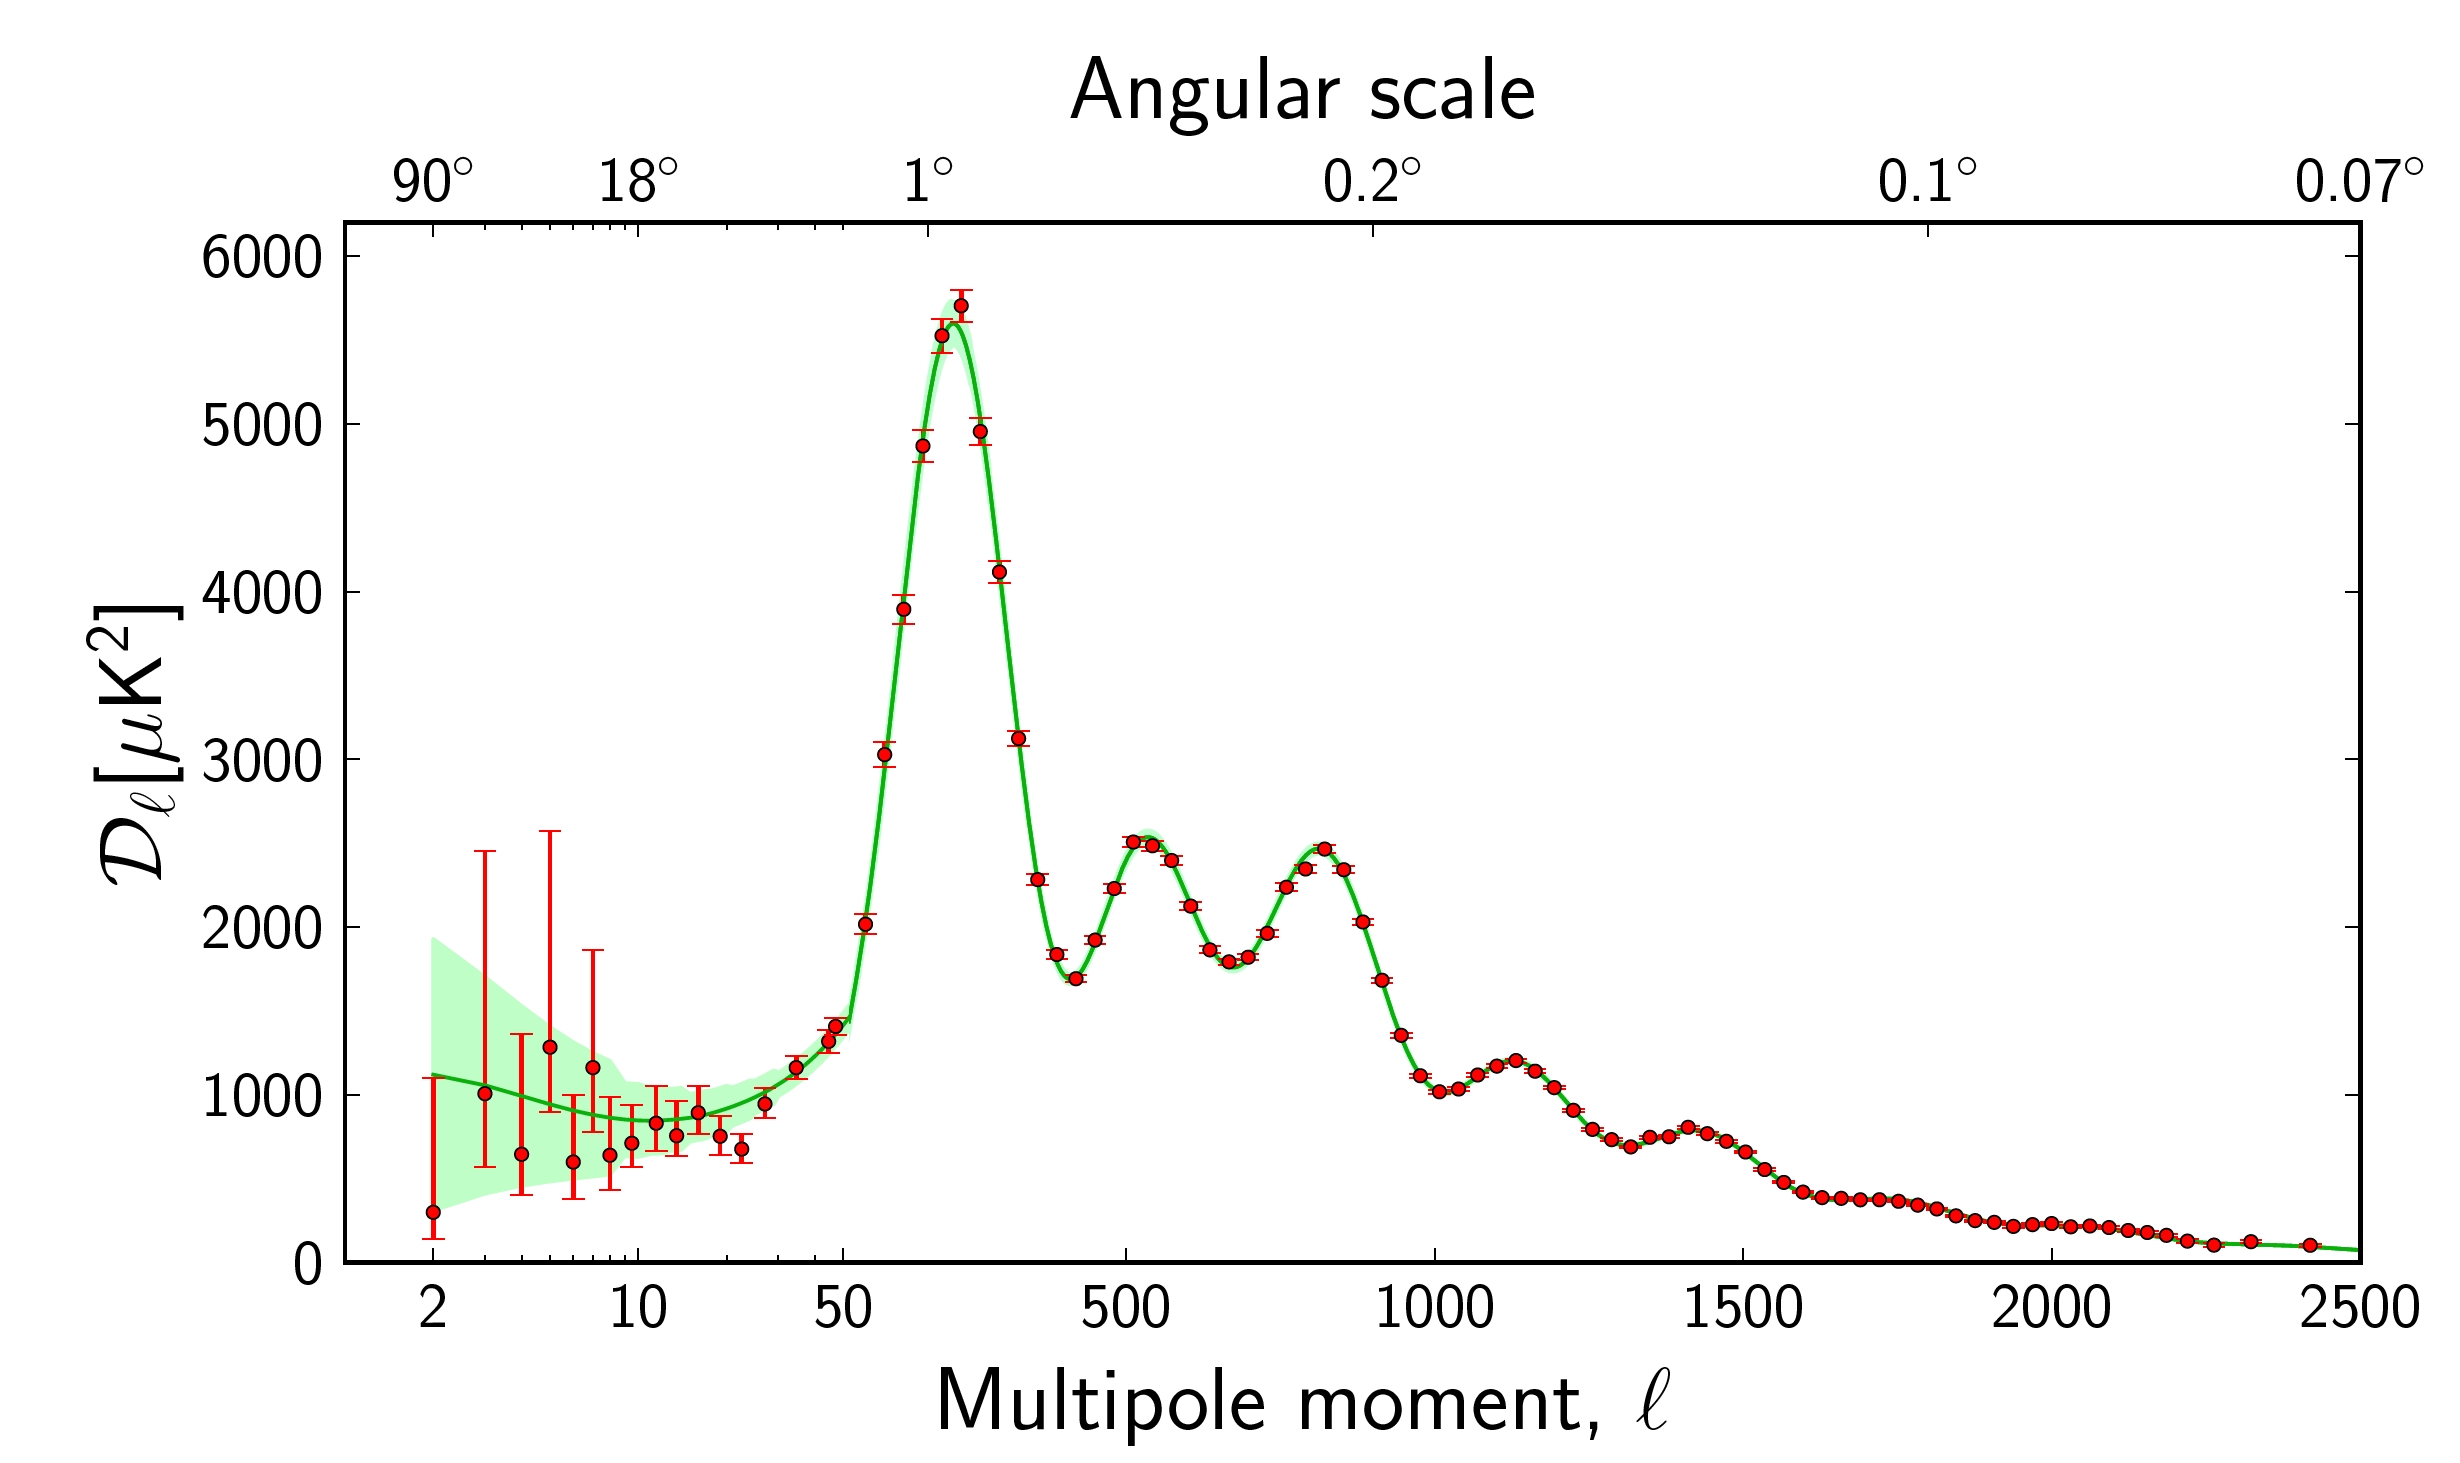
\includegraphics[width=\textwidth]{CMBanisotropies.jpg}
  \caption[CMB anisotropies measured by the Planck experiment]{Angular power spectrum of CMB temperature anisotropies as a measured bythe Planck satellite. Data are shown as red points with the best fit \LCDM cosmological model shown as a green line. Reproduced from Ref.~\cite{PlanckI:2013}.}
  \label{fig:intro:CMB}
\end{figure}


\begin{table}

  \begin{center}
	\begin{tabular}{cc}
        \hline\hline
        Parameter & 68\% limits \\
        \hline
        $\Omega_\Lambda$ & 0.686 $\pm$ 0.020 \\
        $\Omega_m h^2$ & 0.1423 $\pm$ 0.0029 \\
        $\Omega_b h^2$ & 0.02207 $\pm$ 0.00033 \\
        $\Omega_c h^2$ & 0.1196 $\pm$ 0.0031 \\
        \hline\hline
	\end{tabular}
  \end{center}
  \caption[Cosmological parameters obtained by the Planck Collaboration]{Energy density $\Omega$ of the cosmological constant ($\Lambda$), total matter ($m$), and separate baryonic ($b$) and cold dark matter ($c$) components in units of the critical density, as obtained by the Planck Collaboration \cite{PlanckXVI:2013}. The Hubble parameter is defined as $H_0 = 100 \,\,h \, \textrm{km s}^{-1} \textrm{Mpc}^{-1}$.}
  \label{tab:intro:Planck}
\end{table}

However, the evidence for dark matter is not purely cosmological. In 1933, Zwicky measured the velocity dispersion of galaxies in the Coma cluster \cite{Zwicky:1933}. An application of the Virial Theorem indicated a gravitational mass in the cluster which was several hundred times bigger than that expected from the luminosity of the member galaxies. It is now known that some of this mass is in the form of hot ($\sim$1 million K), X-ray emitting intracluster gas \cite{Sanders:2013}. Nonetheless, a discrepancy remains; current estimates of the mass-to-light ratio of the Coma cluster give a value of roughly 150 times that of the Sun \cite{Fusco-Femiano:1994,Makino:1994}. The Coma cluster does not appear to be unusual. Measurements of the masses of a large number of galaxy clusters using gravitational lensing \cite{Okabe:2013}, X-ray observations \cite{Ettori:2013} and dynamical estimates \cite{Carlberg:1995} indicate that a significant fraction of a cluster's mass must be dark.

The success of the \LCDM paradigm is also borne out in results from N-body simulations. These simulations track the evolution of structure in the universe by modeling the dynamics and gravitational interactions of a large number of particles starting from some initial conditions. These may be cosmological simulations, tracing the collapse of the initial density perturbations after decoupling (such as the the Millenium simulation \cite{Springel:2005}), or galaxy-scale simulations, tracing the formation and growth of a small number of galaxies starting from initial conditions at intermediate redshift (such as the Via Lactea \cite{Diemand:2006} and Aquarius \cite{Springel:2008} simulations).

Many N-body simulations are DM-only, simulating only the gravitational dynamics of collisionless particles. However, an increasing number are incorporating baryonic physics such as gas dynamics, as well as stellar evolution, chemical enrichment and a variety of feedback processes (see e.g.~\cite{Mollitor:2014,Vogelsberger:2014}). Appropriately accounting for these factors is extremely complex and in some cases the strength of these processes is unknown and must be tuned in the simulations to match observations \cite{Vogelsberger:2013}. Due in part to these difficulties, the impact of baryonic physics on the formation of galaxies and the properties of DM haloes is still uncertain (see for example Refs.~\cite{Martizzi:2012,Pillepich:2014}). I will revisit this topic - and its consequences for the direct detection of dark matter - in Chapter~\ref{ch:DD}.

A variety of sophisticated computational techniques (such as smoothed particle hydrodynamics \cite{Stinson:2010}, adaptive mesh refinement \cite{Norman:1999} and moving mesh cosmology \cite{Springel:2010}) have been employed and refined to make such simulations computationally feasible and to allow higher and higher resolutions to be reached. In spite of this, computational limitations mean that the highest resolution simulations still use `particle' masses of the order of $10^5 M_{\odot}$ \cite{Pillepich:2014}, many orders of magnitude more massive than the $O$(GeV-TeV) particles expected to make up the universe's dark matter.

In spite of this, a consistent picture has emerged from a vast array of N-body simulations. The distribution of galaxies observed in large scale structure surveys matches that predicted by N-body simulations over a range of distance scales \cite{Springel:2005}. In addition, N-body simulations have begun to accurately reproduce the observed populations of elliptical and spiral galaxies \cite{Vogelsberger:2014}, as well as obtaining Milky Way-like simulated galaxies \cite{Mollitor:2014}. This ability of simulations containing DM to reproduce structures observed in the Universe is further evidence in support of the DM paradigm. Such is the accuracy of N-body simulations that they can be used to generate mock galaxy catalogues which allow statistical and systematic errors to be assessed in real galaxy surveys \cite{Lemson:2006}.



Further evidence for dark matter comes from observations of the rotation curves of spiral galaxies. In particular, the circular velocity of stars in these galaxies is observed to be approximately constant out to large galactocentric distances \cite{Begeman:1991,Persic:1996}. In fact, observations of hydrogen 21cm emission indicate that the constancy of the circular velocity extends well beyond the optical edge of galaxies \cite{Bosma:1981a, Bosma:1981b}.

This is shown schematically in Fig.~\ref{fig:intro:RotationCurves}. The majority of the mass of the luminous disc is concentrated at small radii, suggesting that there should be a Keplerian decay of the circular velocity at large radii: $v \sim r^{-1/2}$. However, the inclusion of an approximately spherically symmetric, non-luminous dark matter halo can reconcile this expectation with the observed flat rotation curves. The density profiles $\rho(r)$ required to provide a good fit to rotation curve data may be consistent with those obtained from N-body simulations, such as the Navarro-Frenk-White profile

\begin{equation}
\label{eq:intro:NFW}
\rho(r) = \frac{\rho_0}{r/R_s(1 + r/R_s)^2}\,,
\end{equation}
which is described by a characteristic density $\rho_0$ and scale radius $R_s$. However, as we discuss in Sec.~ref{sec:intro:problems}, better fits may be obtained by so-called `cored' density profiles. The rotation curve of the Milky Way itself has also been studied \cite{Deason:2012,Lopez-Corredoira:2014,Bhattacharjee:2014} and found to be almost flat. Using a variety of techniques, it is also possible to measure a non-zero DM density near the Sun's position. An understanding of this density has significant implications for the study of dark matter detection and we defer a detailed discussion to Chapter~\ref{ch:DD}.

\begin{figure}[h]

  \centering
  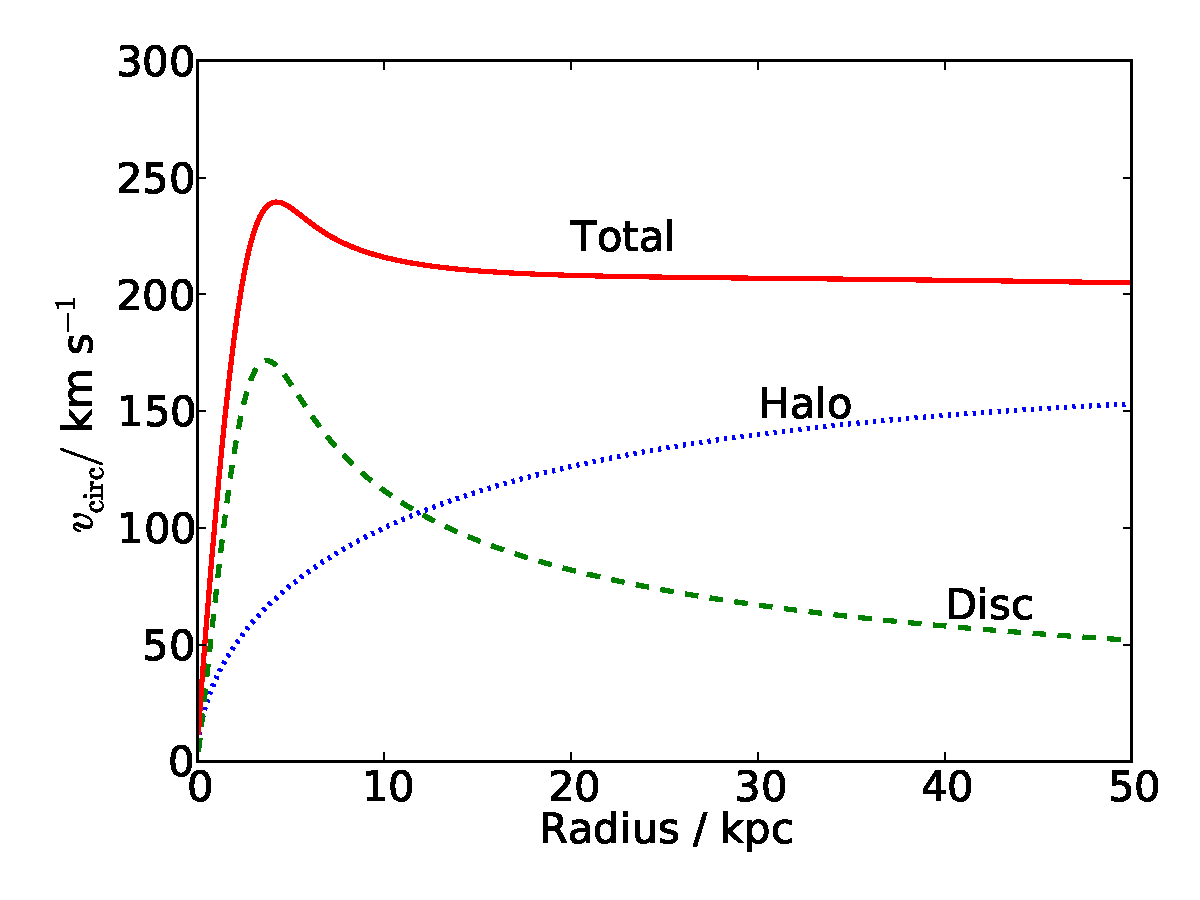
\includegraphics[width=0.8\textwidth]{RotationCurve.pdf}
  \caption[Schematic illustration of galaxy rotation curves]{Schematic illustration of galaxy rotation curves (circular velocity as a function of galactocentric distance). The contribution to the circular velocity from the luminous disc (green dashed line) and dark matter halo (red dotted line) are shown, as well as the total circular velocity (solid blue line). }
  \label{fig:intro:RotationCurves}
\end{figure}

We see that evidence for dark matter appears over a wide range of distance scales, from the cosmological horizon down to our own Milky Way. Dark matter is required to explain the formation and growth of large scale structure, the dynamics of both galaxies and galaxy clusters and the anisotropic temperature distribution of the CMB among others. In spite of this, there remain several problems and unanswered questions with the dark matter paradigm.


\subsection{Problems with dark matter}
\label{sec:intro:problems}
There have emerged several issues with the dark matter dominated model of structure formation as studied with N-body simulations. For example, DM-only simulations predict the existence of a large number of massive subhalos around Milky Way-size galaxies \cite{Springel:2008}. Using semi-analytical models of galaxy formation Kauffmann \etal \cite{Kauffmann:1993} predicted that a Milky Way-size halo should host over 100 subhalos massive enough to support observable satellite galaxies.  However, the known population of dwarf spheroidal (dSph) satellite galaxies for the Milky Way is on the order of 20 \cite{Walker:2009}, although more ultra-faint satellites are still being discovered (e.g. see Ref.~\cite{Belokurov:2010}). This discrepancy between the predicted and observed amount of substructure in CDM structure formation is often referred to as the `missing satellite problem' \cite{Klypin:1999}.

A related issue is the so-called `too big to fail' problem, which concerns the density of dark matter subhalos. In particular, it is found that the most massive DM subhalos found in N-body simulations are too massive to host the brightest of the Milky Way's dSph satellites \cite{Boylan-Kolchin:2011}. If the observed dSph galaxies are hosted instead by less massive subhalos, this leaves a large number of more massive DM halos which have not yet been accounted for \cite{Garrison-Kimmel:2014}.

Finally, there is also a discrepancy between observed and simulated density profiles for dSphs: the `Core-Cusp' problem (for a review, see Ref.~\cite{deBlok:2009}). Cosmological simulations indicate that the DM density should be sharply peaked near the centre of low surface brightness and dSph galaxies \cite{Dubinski:1991, Navarro:1996}. In contrast, observations of the rotation curves of a large number of galaxies suggests the presence of a core - a flat dark matter density profile near the centre \cite{Salucci:2001, Donato:2004}. While these results are still under contention (for example, Ref.~\cite{Hayashi:2004} find rotation curves consistent with \textit{cuspy} density profiles), they may indicate a discrepancy between the process of structure formation in the universe and that implied by \LCDM.

A number of possible solutions to these issues have been suggested. Baryonic effects such as dynamical friction and stellar and supernova feedback (see for example Refs.~\cite{Gritschneder:2013, Amorisco:2014,DelPopolo:2014}) can lead to the expulsion of DM from the centres of subhalos, reducing the total halo mass and leading to a flatter central density profile. Others have suggested that a \textit{warm} dark matter model may be a better fit to the data \cite{Moore:1999, Bode:2001, Maccio:2010}, reducing the amount of structure on small scales, as we will discuss in Sec.~\ref{intro:sec:properties}. Whatever the ultimate resolution of these problems, it is clear that dark matter dominated structures such as dSph galaxies are a testing ground for an even more precise understanding of structure formation in the DM paradigm.

There remains one problem which is of a much more theoretical nature. Dark matter is invoked to account for missing mass in a wide range of scenarios. However, this missing mass has not yet been observed indicating that it must interact only very weakly with photons and other particles of the standard model. In fact, as we shall see, there is strong evidence that particles making up the universe's dark matter cannot be baryonic and must originate from beyond the Standard Model of particle physics. In the next section, we investigate what more can be inferred about the nature of particle dark matter and explore some well-motivated candidates.

\todo{MACHOs? MOND?}

\note{Need consistency between `DM' and `dark matter'}

\section{Alternatives to dark matter}

We have discussed a wide range of evidence for the existence of DM, as well as some unresolved problems with the \LCDM paradigm. Here, we consider the possibility that these observations can be explained not by a new matter species but by a modification to gravity. Milgrom \cite{Milgrom:1983a, Milgrom:1983b, Milgrom:1983c} proposed the idea of Modified Newtonian Dynamics (MOND): for accelerations smaller than some characteristic value $a_0$ the usual Newtonian dynamics no longer holds. In particular, for an acceleration $\mathbf{a}$ in a gravitational field $\Phi_N$, these new dynamics can be written
\begin{equation}
\label{eq:intro:MOND}
\tilde{\mu}(|\mathbf{a}|/a_0)\mathbf{a} = -\nabla \Phi_N\,.
\end{equation}
The interpolation function $\tilde{\mu}$ tends to unity for large values (the Newtonian limit) but tends to $|\mathbf{a}|/a_0$ for values $|\mathbf{a}| \ll a_0$ (the MOND limit).

At large distances fromm the centres of galaxies, the acceleration will drop below $a_0$ and Eq.~\ref{eq:intro:MOND} reduces to $a = v_c(r)^2/r = \sqrt{a_0 \nabla \Phi_N}$, where $v_c$ is the circular velocity. Assuming that there is no dark matter content, the mass $M$ enclosed within a radius $r$ becomes constant and we obtain $|\nabla \Phi_N| \approx GM/r^2$. Combining these, we see that

\begin{equation}
\label{eq:intro:TullyFisher}
v_c(r)^4 \approx GM a_o\,,
\end{equation}
independent of radius. Thus, a flat rotation curve is obtained without the need to invoke DM. Moreover, Eq.~\ref{eq:intro:TullyFisher} is the baryonic Tully-Fisher law, which relates the baryonic mass of a galaxy with the asymptotic rotation velocity, and which does not have an obvious origin in DM-based models \cite{Gnedin:2007}. The value for the characteristic acceleration obtained from fits to over 100 galaxies is $a_0 = 1.2 \times 10^{-10} \textrm{ m s}^{-2}$ \cite{Begeman:1991}, which also reproduces the measured proportionality constant in the Tully-Fisher law \cite{McGaugh:2005}.

The phenomological approach of MOND can be recast into a fully covariant theory of modified gravity, known as tensor-vector-scalar (TeVeS) gravity \cite{Bekenstein:2005}. This theory contains new dynamical vector and scalar degrees of freedom and contains a free function, analogous to the interpolation function $\tilde{\mu}$. The formalism for both lensing \cite{Chiu:2005} and cosmological perturbations \cite{Skordis:2006} have both been studied in TeVeS, with perturbations in the new scalar and vector fields allowing structure to form without the need for DM.

How then does MOND compare to DM? MOND can generally give good fits to galaxy rotation curves \cite{Begeman:1991,Sanders:1996,deBlok:1998} and can do so with fewer free parameters than DM halo models. MOND can also reduce the tension between the mass in clusters and the dynamical or lensing masses \cite{Sanders:2002,Angus:2006}, but typically only to within a factor 2, still requiring some collisionless matter to fit data \cite{Dodelson:2006}. However, the biggest problem is that relativistic extensions of MOND have yet to reproduce the features of large scale structure and the CMB with the same success as \LCDM \cite{Slosar:2005,Skordis:2006b,Zuntz:2010}. Though the range of possible extensions is large and the cosmological data may yet be explained within such a framework, we will focus here on the DM paradigm for explaining such observations.

%http://arxiv.org/abs/1307.3937

\note{Universe}

\section{Properties of dark matter}
\label{intro:sec:properties}

Beyond its gravitational contribution to the Universe, we appear to know little about the nature of particle dark matter. However, the success of modern cosmology and the lack of a confirmed detection so far means that we do have a grasp on some of the properties of any potential candidate.

For example, DM can have no significant electromagnetic charge, otherwise it would have been seen in a range of searches \cite{Kudo:2001,Perl:2001,Gninenko:2007,Melchiorri:2007}. DM carrying bare color charge can also be excluded due to the disruption it would cause to galaxy formation \cite{Natarajan:2002} and the formation of the CMB \cite{Chen:2002}. Any particle candidate must also be long-lived - otherwise it cannot play the role of dark matter today. For models in which DM is not indefinitely stable, this allows us to place stringent limits on the lifetime of the DM particle \cite{Amigo:2009,Bell:2010}. %\note{These don't actually come from those arguments, but K.}

In an effort to summarise what is known about dark matter, Taoso \etal \cite{Taoso:2008} present a `10-point test' which must be passed by any particle before it can be considered as a viable dark matter candidate. Here, I will briefly discuss three of these points, namely, that the DM candidate must be cold, produced with the appropriate relic density and compatible with primordial nucleosynthesis.

\subsection{Coldness}

Dark matter cannot be hot. That is, DM must have been travelling non-relativistically when it decoupled from the thermal bath in the early universe. The typical speed of DM particles in the early universe defines the so-called \textit{free-streaming length}. Below this length-scale, density perturbations are suppressed due to Landau damping \cite{Bond:1983}. For non-relativistic species, this free-streaming length scales as $m_\chi^{-1/2}$ for thermal relics of mass $m_\chi$ \cite{Boyanovsky:2008} For particle candidates which are too light - and which therefore travel too quickly after decoupling - small scale structures cannot form and cannot match the distribution of structures we see today. In practise, this typically means that DM cannot have a mass greater than around 1 keV \cite{Narayanan:2000}. It is typically assumed that dark matter is significantly heavier than this, decoupling ultra-non-relativistically in the early universe, rendering it cold.  \textit{Warm} dark matter candidates with keV-scale masses have been suggested to explain the subhalo structures at the scale of dSph galaxies (as has already been discussed). However, \textit{hot} dark matter, which decouples at relativistic speeds, is strongly-constrained and cannot make up more than around 1\% of the total dark matter component \cite{Abazajian:2005, dePutter:2012}.


\begin{comment}
\subsection{Neutrality}

\todo{Condense this into a couple of sentences in the section intro...}

The possibility that charged massive particles (CHAMPs) may account for dark matter was proposed by De Rujula \etal \cite{DeRujula:1990}. Such particles be free and stable or may instead bind with electrons or positrons to form heavy neutral hydrogen-like objects. However, null searches for anomalous hydrogen in sea water \cite{Kudo:2001} and anomalous heavy elements \cite{Hemmick:1990}, as well as searches for CHAMPs in cosmic ray experiments \cite{Perl:2001} indicate that CHAMPs must be present in negligible densities in the Milky Way for masses in the range $10-10^8$ GeV. Millichared DM is also strongly constrained. Searches for neutrino magnetic moments in reactor experiments exclude DM with charge greater than $10^{-5} e$ for keV-scale masses and below \cite{Gninenko:2007}. Searches for distortions in the CMB caused by the interactions of millicharged particles limit the DM charge to be less than $10^{-7} e$ for masses of 1 eV and below \cite{Melchiorri:2007}.

Could DM particles carry a colour charge? In this case, DM particles would interact strongly with particles of the SM. Such strong interactions may disrupt galaxy formation \cite{Natarajan:2002}, distort the CMB due to scattering off baryons \cite{Chen:2002} and have been strongly constrained by experimental searches with the X-ray Quantum Calorimeter \cite{Erickcek:2007} and direct detection experiments \cite{Albuquerque:2004}. %\note{What about weak hypercharge?}

We are left with the conclusion that (without a mechanism for evading the above constraints \cite{AnExample}) DM particles must carry no (or almost no) conventional electromagnetic, weak or strong charge. This rules out all SM particles as accounting for DM hinting strongly that these particles must derive from theories of physics beyond the Standard Model.

%\note{What about current constraints on `dark atoms'?}
\end{comment}
\subsection{Relic density}

In order to account for the dark matter in the universe, a good candidate must be produced in the early universe with sufficient abundance to match the currently observed value $\Omega_c h^2 = 0.1196 \pm 0.0031$ (see Table~\ref{tab:intro:Planck}). If produced with a smaller abundance, the candidate cannot account for the entirety of the universe's dark matter (though it could still contribute, along with other candidates, as in Ref.~\cite{Feldman:2010}). If on the other hand, it is produced with too great an abundance, it could threaten to exceed the DM density constraint set by Planck and overclose the universe.

The standard scenario for the production of dark matter is referred to as thermal freeze-out \cite{Kolb:1990}. In this scenario, DM particles remain in kinetic and chemical equilibrium with SM particles in the very early universe by scattering and annihilation processes. Their number density $n$ follows a Maxwell-Boltzmann distribution

\begin{equation}
n \sim (m/T)^{3/2} \exp(-m/T)\,,
\end{equation}
for a mass $m$ and temperature $T$. As the universe expands, however, the particles become diluted, reducing the interaction rate until eventually the DM particles become decoupled from the SM particles and are `frozen-out.' They are then left with the abundance they had when they decoupled, which is further diluted by the expansion of the universe to become the abundance we see today. The exact relic abundance depends on $\langle \sigma_\mathrm{ann} v\rangle$, the average annihilation cross section of the DM particles (weighted by the DM speed). If this is small, DM will decouple early when the temperature of the universe is still high, leading to a large relic abundance. If the annihilation cross section is large, DM will remain in equilibrium  for longer, even as the particles become more and more diluted. The DM then freezes out later, with a lower temperature and lower relic abundance. The resulting relic abundance for GeV-scale DM is given approximately by:
%\todo{Make a simple figure for this.} This process is illustrated schematically in Fig.~\ref{intro:fig:freezeout}.
\begin{equation}
\Omega_c h^2 \approx \frac{3 \times 10^{-27} \textrm{ cm}^{3} \textrm{ s}^{-1}}{\langle \sigma_\mathrm{ann} v \rangle}\,,
\end{equation}
leading to a canonical value of around $\langle \sigma_\mathrm{ann} v \rangle \approx 3 \times 10^{-26} \textrm{ cm}^{3} \textrm{ s}^{-1}$ for the annihilation cross section. This coincides well with the value expected for particles with weak-scale interactions (so-called weakly interacting massive particles, or WIMPs), leading some to refer to this argument as the WIMP miracle. In reality, the full differential equations describing the DM number density must be solved \cite{Gelmini:2010}, accounting for co-annihilations \cite{Griest:1991}, which may boost the total cross section. However, the simplicity of this scenario make cold thermal relics an attractive candidate for DM.

Dark matter may also achieve the correct relic abundance through a variety of other mechanisms. `Freeze-\textit{in}' \cite{Hall:2009} involves particles which interact so weakly (termed feebly interacting massive particles, FIMPs) that they never reach equilibrium. Instead, a relic population is built up gradually through the production of FIMPs by annihilation of SM particles. In contrast to the freeze-out scenario, the relic abundance of FIMPs increases with increasing annihilation cross section. Dark matter may also be produced gravitationally from vaccuum fluctuations during and after inflation \cite{Chung:1998, Kuzmin:1998} or from the decays of heavier meta-stable particles (e.g. Ref.~\cite{Gherghetta:1999}). These possibilities open up the range of candidates which may be considered to include much lighter or much heavier particles than the freeze-out scenario alone might allow.

%WIMPzillas - gravitational
%SuperWIMPs (gravitinos...) - decays

\subsection{Primordial nucleosynthesis}

%\note{Need more refs here...}

Primordial nucleosynthesis (or Big Bang Nucleosynthesis, BBN) describes the production of light nuclei in the first few minutes after the big bang. By solving a set of coupled Boltzmann equations describing the nuclear reactions of protons, neutrons and light nuclei, we can obtain the primordial abundances of these light nuclei and compare with the inferred values \cite{Tytler:2000}. Significantly, these abundances depend strongly on the baryon-photon ratio $\eta$ and therefore the total baryon density. Fits to data lead to the result $\Omega_b h^2 = 0.017 - 0.024$ \cite{Fields:2006}, independent of the value obtained from CMB measurements (Table~\ref{tab:intro:Planck}). Thus, the baryonic matter can make up only a fraction of the total matter density of the universe. We are led to conclude that particle dark matter must consist of some non-baryonic particle.

%\note{Combine this with the `neutrality' constraint and we see that there are no SM particles (or their spartners?) with the correct quantum numbers.}

The results of BBN are also very sensitive to light new species, which can alter the number of relativistic degrees of freedom in the early universe and therefore affect the expansion rate. These include, for example, gravitinos \cite{Maggiore:2000} and right-handed neutrinos \cite{Cyburt:2005}. BBN therefore provides strong constraints on the parameters of such models. In addition, the decay of dark matter particles into electromagnetic or hadronic showers during nucleosynthesis can drastically change the primordial abundances of the light elements. BBN can therefore be used to constrain models in which dark matter undergoes early decays (or in which dark matter is produced by the decays of heavier particles) \cite{Jedamzik:2006}.

%\note{What about stating some of the constraints on Nv?}

\section{Particle dark matter candidates}
\label{intro:sec:candidates}

%\note{Make an explicit distinction between WIMPs and non-WIMPs?}

While \textit{valid} DM candidates need only satisfy the conditions and constraints which have already been discussed, \textit{well-motivated} candidates should derive sensibly from some physical model. In fact, dark matter candidates can be found in a wide range of models of particle physics beyond the standard model. As has already been discussed, massive particles with GeV-scale masses and weak-scale interactions are attractive for obtaining the correct DM relic density. Such a WIMP candidate may be provided by the lightest supersymmetric particle (LSP) in supersymmetric theories \cite{Jungman:1995}. In supersymmetry, each of the known SM particles has a supersymmetric partner (or `spartner'), with bosons having fermionic partners and vice versa - this additional symmetry is often invoked to help alleviate the hierarchy problem \cite{Kane:2011}. In models which possess R-parity (which may be required to protect the proton from decay), particles carry R-parity 1 while supersymmetric particles (`sparticles') carry R-parity -1. This means that the lightest sparticle cannot decay into SM particles and is therefore stable, making it a promising DM candidate.

%\note{Does this hold JUST for the MSSM?}

Depending on the parameters of the supersymmetric theory, there are many possibilities for which sparticle will be the LSP. One popular and well-studied possibility is the neutralino $\chi$ \cite{Ellis:1984}, which is a linear combination of the neutral supersymmetric partners of the $W$ and $B$ with the CP-even higgsinos. The properties of the neutralino can vary dramatically depending on the mixing between these different components and the underlying supersymmetric parameters \cite{Shakya:2013}. In other cases, the LSP may be sneutrino \cite{Choi:2013}, a partner of the standard model neutrino. %\todo{Say more about sneutrinos...are they excluded already by direct searches?}
Another alternative is the gravitino, in which case it may be produced gravitationally in the early universe with a mass greater than $10^{12}$ GeV, leading to the title `WIMPzilla' \cite{Kolb:1998}.

WIMPs also arise in theories of universal extra dimensions, in which the additional dimensions are compactified, leading to a tower of excited states of the standard model particles \cite{Duff:1994}. These `Kaluza-Klein' (KK) particles also possess a KK-parity, which means that the lightest KK particle (LKP) is stabilised \cite{Appelquist:2001}. One possibility for the LKP is the first excitation of the $B$ weak hypercharge boson, $B^{(1)}$. In this case, the WIMP would be a spin-1 particle with a mass of around 1 TeV (in order to be produced thermally with the correct relic abundance) \cite{Cheng:2002}. It has also been shown that the first KK excitations of the photon and neutrino are viable DM candidates if they also have masses at the TeV scale \cite{Servant:2002}. In contrast to the LSP, the LKP is described by a relatively small parameter space and may be more easily constrained by upcoming experiments \cite{Bergstrom:2009}.

In light of the problems with models of dark matter structure formation on small scales, there are several candidates which may be attractive for constituting warm dark matter. While standard neutrinos (with masses of a few eV \cite{Amsler:2008}) cannot account for a large fraction of the dark matter, keV-scale sterile neutrinos may be viable \cite{Dodelson:1994}. Sterile neutrinos interact with ordinary matter via neutrino mixing rather than via electroweak interactions. While attractive for providing warm dark matter, non-thermal production \cite{Shi:1999} or multiple sterile neutrinos species \cite{Asaka:2006} may be required to avoid many astrophysical and cosmological constraints \cite{Hansen:2002,Abazajian:2006}.

Another non-WIMP candidate is the axion. The axion was originally introduced by Peccei and Quinn \cite{Peccei:1977} to solve the strong CP problem. It was observed that this spin-zero particle should be produced in abundance in the early universe via the `misalignment mechanism' and, for masses in the range $10^{-5} - 10^{-3}$ eV, can account for the cosmological dark matter \cite{Raffelt:1995}. It was recently noted that axion dark matter would thermalise and form a Bose-Einstein condensate, acting as cold dark matter at late times \cite{Sikivie:2009}, as well as explaining anomalies in the alignment of CMB multipoles \cite{Copi:2010}. Also of interest are axion-like particles (ALPs), which emerge naturally in string theory and are expected to span many orders of magnitude in mass and coupling strength \cite{Arvanitaki:2009}.

As is clear from this discussion, there are a wide range of well-motivated candidates for the dark matter in the universe. Some further examples include WIMPless dark matter \cite{Feng:2010}, mirror dark matter \cite{Foot:2014} and little Higgs dark matter \cite{Birkedal:2006}, as well as minimal approaches to DM \cite{Cirelli:2007}. In this work, we focus on the WIMP, not only because of its popularity and generic nature, but because of the large number of experimental searches which provide sensitivity to WIMP dark matter.


% From PDM: arXiv:1001.3651,  arXiv:1002.3828. What about minimal approaches
The final condition appearing in the `10-point test' of Taoso \etal asks the question `Can it be probed experimentally?' While it may be possible that DM interacts only gravitationally, a wide variety of proposed candidates can interact (however weakly) with the particles of the standard model. While the experimental accessibility of a given DM candidate is not a strict necessity, it allows models to be tested (and either falsified or confirmed) beyond the hypothesis stage. In the next section, we explore the different avenues by which models of particle dark matter may be probed.

\section{Detection of dark matter}

Many of the candidates which have been discussed are expected to interact weakly with the particles of the Standard Model (SM). We note in particular that dark matter particles which are produced by thermal freeze-out in the early universe must have interactions with SM particles in order to maintain thermal and kinetic equilibrium. These interactions are mediated by Feynman diagrams which can be represented (schematically) as in Fig.~\ref{intro:fig:diagrams}. The existence of production, annihilation and scattering processes between DM and SM particles provides a window into the possible detection of particle DM. Each of these processes leads to a distinct detection strategy, referred to as collider, indirect and direction detection.

\begin{figure}[t]

	\centering
        \subbottom[Production]
                {\begin{fmffile}{DM1}
		\setlength{\unitlength}{0.08cm}
		\raisebox{0.2\height}{
                \begin{fmfgraph*}(40,25)
		\fmfleft{i1,i2}
		\fmfright{o1,o2}
		\fmf{fermion}{i1,v1}
		\fmf{fermion}{v1,o1}
		\fmf{fermion}{i2,v1}
		\fmf{fermion}{v1,o2}
		\fmflabel{$\psi$}{i1}
		\fmflabel{$\psi$}{i2}
		\fmflabel{$\chi$}{o1}
		\fmflabel{$\chi$}{o2}
		\fmfblob{.16w}{v1}
		\end{fmfgraph*}}
		\end{fmffile}\label{intro:fig:diagramsa}}
        \subbottom[Annihilation]
                {\begin{fmffile}{DM2}
		\setlength{\unitlength}{0.08cm}
                \raisebox{0.2\height}{
		\begin{fmfgraph*}(40,25)
		\fmfleft{i1,i2}
		\fmfright{o1,o2}
		\fmf{fermion}{i1,v1}
		\fmf{fermion}{v1,o1}
		\fmf{fermion}{i2,v1}
		\fmf{fermion}{v1,o2}
		\fmflabel{$\chi$}{i1}
		\fmflabel{$\chi$}{i2}
		\fmflabel{$\psi$}{o1}
		\fmflabel{$\psi$}{o2}
		\fmfblob{.16w}{v1}
		\end{fmfgraph*}}
		\end{fmffile}\label{intro:fig:diagramsb}}
         \subbottom[Scattering]
                {\begin{fmffile}{DM3}
		\setlength{\unitlength}{0.08cm}
                \raisebox{0.2\height}{
		\begin{fmfgraph*}(40,25)
		\fmfleft{i1,i2}
		\fmfright{o1,o2}
		\fmf{fermion}{i1,v1}
		\fmf{fermion}{v1,o1}
		\fmf{fermion}{i2,v1}
		\fmf{fermion}{v1,o2}
		\fmflabel{$\psi$}{i1}
		\fmflabel{$\chi$}{i2}
		\fmflabel{$\psi$}{o1}
		\fmflabel{$\chi$}{o2}
		\fmfblob{.16w}{v1}
		\end{fmfgraph*}}
		\end{fmffile}\label{intro:fig:diagramsc}}
   \caption[Schematic dark matter interactions]{Schematic interactions between dark matter particles $\chi$ and standard model particles $\psi$.}
\label{intro:fig:diagrams}
\end{figure}

\subsection{Collider production}

%\note{Elaborate and actually explain more of this section. Add more from the PDM...}
%\note{What about actual current limits, nothing seen yet?}
%\note{What about kinematic endpoints...?}

Searches for dark matter at the particle colliders such as the LHC rely on processes such as Fig.~\ref{intro:fig:diagramsa}, in which SM particles annihilate to produce dark matter particles. However, the weak interactions of the DM means that once produced, it will escape the detectors around the interaction point without being observed. Thus, collider searches for dark matter must look for other signatures.

One approach is to look for signatures which are characteristic of a particular theory. For example, looking for evidence of KK states which are expected in theories of universal extra dimensions \cite{Edelhauser:2013, Kakuda:2013}, or searching for particle signatures from decay chains which are expected from supersymmetry \cite{ATLAS:2013, CMS:2013}. While this allows constraints to be placed on specific models, the range of models may be large, meaning that each must be constrained separately.

%Fits to CMSSM using LHC data...

An alternative approach is to look for deviations from the SM expectation and use this to place limits on the operators of an effective field theory (see e.g.~\cite{Zhang:2011}). One possible signature is to look for the pair production of DM states, with initial state radiation of a SM particle. It is then possible to search for this initial state radiation (which may be a single jet or a single boson or lepton, depending on which particle was radiated). By combining all the possibilities for the form of the initial state radiation, we can place bounds on the effective operators which govern SM-DM interactions \cite{Zhou:2013}. \note{Mention actual numbers/results.} It is also possible to look for more general missing energy signatures \cite{Fox:2011a}, in which energy is carried away by the dark matter particle produced.

One advantage of this effective operator approach is that these bounds can be translated into limits on signals at direct and indirect experiments, allowing collider results to be incorporated with other experimental searches in a complementary fashion \cite{Baer:2009}. However, it has been noted that caution must be exercised in naively applying the field theory approach at the LHC as well as in translating this to other search channels \cite{Buchmueller:2013,Busoni:2013}.

So far, there has been no evidence observed for the production of dark matter particles at the LHC \cite{}. The non-observation of supersymmetry at the LHC has also begun to place some tension on SUSY dark matter models \cite{Bechtle:2012}, though they are not yet excluded \cite{Bechtle:2013}. The proposed International Linear Collider (ILC) \cite{Barish:2013} should be able to explore more of the possible dark matter parameter space \cite{Schmeier:2013,Chae:2013}


\subsection{Indirect detection}


The possibility of dark matter annihilation into SM particles (as described in Fig.~\ref{intro:fig:diagramsb}) means that DM may be detected indirectly, by searching for these excess annihilation products (and related decay products). Some searches aim to look for the contribution of these products to signals obtained over large survey areas. The Fermi-LAT collaboration have published limits on searches for spectral lines and contributions to the diffuse background of gamma-rays \cite{Ackermann:2012}. Cosmic ray experiments such as PAMELA \cite{Boezio:2009} have aimed to measure the $p^{\pm}$ and $e^{\pm}$ abundances in cosmic rays. The AMS experiment \cite{Aguilar:2013} has recently reported a rise in the cosmic ray positron fraction at energies above 10 GeV, which has been interpreted as tentative evidence for dark matter annihilations (see e.g. Ref.~\cite{Ibarra:2014}). For charged cosmic rays, astrophysical magnetic fields deflect the paths of particles, meaning that it can be difficult to resolve individual sources \cite{Medina:1998}.

 In contrast, photon searches allow specific locations to be targeted. Because the signal rate is proportional to the DM annihilation rate (along the line of sight), the potential signal scales as the square of the dark matter density. Thus, searching in areas where the DM density is expected to be high can boost the signal rate significantly \cite{Lavalle:2008}. As has already been discussed, dSph galaxies are dark matter dominated objects and thus represent promising targets for indirect searches. A survey of 25 Milky Way satellite galaxies by the Fermi-LAT telescope \cite{Ackermann:2014} has so far found no significant gamma-ray signal. However, upper limits on the annihilation cross section are in some cases close to the thermal freeze-out value of $\langle \sigma_\mathrm{ann} v \rangle \approx 3 \times 10^{-26} \textrm{ cm}^{3} \textrm{ s}^{-1}$, depending on the WIMP mass and annihilation channel. By optimising search regions near the centre of the Milky Way for maximum signal-to-noise, Weniger recently found a bump in the gamma-ray spectrum of Fermi-LAT data around 130 GeV \cite{Weniger:2012}. However, subsequent analysis has found that this feature may be a systematic effect in the detector \cite{Bloom:2013} and that it is difficult to reconcile with conventional models for dark matter \cite{Buchmuller:2012, Cohen:2012}.

Perhaps more promising is a different gamma ray signal coming from the inner regions of the Galaxy, peaking at energies around 1-3 GeV \cite{Goodenough:2009,Hooper:2011}. Fits of the data point towards a dark matter particle with a mass of 31-40 GeV, annihilating predominantly to $b\bar{b}$ with a cross section of $\langle \sigma v \rangle = (1.4-2.0) \times 10^{-26}$ cm$^3$ s$^{-1}$, approximately matching the value required for a particle created by thermal freeze-out in the early universe. While it has been suggested that this signal is actually consistent with known sources \cite{Boyarsky:2010} or as yet unresolved astrophysical sources \cite{Abazajian:2011}, further analysis has shown that the signal matches the spectrum and morphology expected from DM annihilation \cite{Daylan:2014}. Confirmation of the signal may have to wait until it is corroborated by independent observations, for example a DM annihilation signal from dSph galaxies.

The sensitivity of gamma ray searches can be extended up to TeV-scale masses with ground-based Imaging Atmospheric Cherenkov Telescopes (IACTs). These work by imaging the Cherenkov radiation from charged particles produced when high energy gamma rays impinge on the atmosphere. The current generation of IACTs - HESS \cite{Abramowski:2013}, MAGIC \cite{Aleksic:2014} and VERITAS \cite{Acciari:2010} - have been used to conduct searches for line-like gamma ray spectra as well as searches for signals from dwarf galaxies. However, these limits are typically around two orders of magnitude above the thermal cross section. The planned Cherenkov Telescope Array (CTA) may be able to probe down to this thermal cross section for high WIMP masses \cite{Doro:2013}.
%\note{What about the inner galaxy?}

%NOTE: Water cherenkov telescopes...

Another potentially rich source of DM annihilations are the Sun and Earth. DM particles may scatter with nuclei in these bodies, losing energy and eventually becoming captured. Eventually, the DM sinks to the centre of the object and annihilates. The only annihilation products which can escape are neutrinos, which can then be detected at neutrino telescopes such as ANTARES \cite{Zornoza:2012} and IceCube \cite{Aartsen:2013b}. Because the neutrino flux depends on the scattering rate of DM with nuclei, such signals can probe similar (but complementary) parameter spaces to direct detection experiments. We treat this subject in more detail in Chapter~\ref{ch:NT}.




%\todo{ICECUBE SEARCHES FOR DM ANNIHILATION IN GALAXIES AND CLUSTERS \cite{Aartsen:2013}}

\subsection{Direct detection}

Processes described by the diagram in Fig.~\ref{intro:fig:diagramsc} lead to the possibility of scattering between DM and SM particles. The principle of direct detection is to look for nuclear recoils due to this scattering in a dedicated detector \cite{Goodman:1985,Drukier:1986}. WIMPs with GeV-scale masses and speeds $v \sim 10^{-3} c$ are expected to produce keV-scale nuclear recoils. In addition, due to the expected low cross section for such interactions, the predicted rate is less than around 1 event per year per kg of detector mass. Detecting such rare, low energy recoils requires not only large ton-scale detectors, but also sophisticated methods for discriminating signal from background.

Several direct detection experiments have claimed a tentative signal, such as DAMA/LIBRA \cite{Bernabei:2010}, CoGeNT \cite{Aalseth:2011a, Aalseth:2011b} and CRESST-II \cite{Stodolsky:2012}. However, these are in tension with null results from other experiments such as the recent LUX report \cite{Akerib:2014}. Due to a range of uncertainties in nuclear physics, particle physics and astrophysics it may be possible to reconcile these results. In any case, a firm understanding of these uncertainties will be necessary to build a coherent picture from future results. The interpretation of direct detection data will be the main focus of this work and the main subject of Chapter~\ref{ch:DD}.

%\todo{Say something about complementarity between these 3.}

\subsection{Conclusions}

The \LCDM paradigm has enjoyed great success in explaining observations from galactic to cosmological scales. While discrepancies with observations on smaller scales remain, these are being actively pursued and may prove to be valuable testing grounds for the process of dark matter structure formation.

The identity of dark matter is unknown and cannot be accounted for by any of the known standard model particles. Even so, we know that it must be neutral, long-lived and cold (or possibly warm) and that it must pass a variety of stringent tests coming from BBN and the CMB. There is no lack of well-motivated CDM candidates, including the lightest supersymmetric and Kaluza-Klein particles, sterile neutrinos, axions and many more. We have focussed on the search for weakly interacting massive particles (WIMPs) and described how direct, indirect and collider searches have been used to place limits on the WIMP parameters and soon hope to make the first non-gravitational detection of DM.


\chapter{Direct detection of dark matter}

\section{Introduction}

\note{Definitely need to include a little bit about what the event rates actually look like. Some plots and stuff...}

The idea that particle dark matter (DM) may be observed in terrestrial detectors was first proposed by Goodman and Witten in 1985 \cite{Goodman:1985} and by Drukier, Freese and Spergel in 1986 \cite{Drukier:1986}. If DM can interact with particles of the Standard Model, the flux of DM from the halo of the Milky Way should be large enough to cause measureable scattering from nuclei. If the subsequent recoils can be detected and their energy spectrum measured, it should be possible to infer some properties of the DM particles.

However, the expected event rate for keV-scale recoils at such a detector would be of the order of $10^{-10}$ events per kg of detector material per day per keV recoil energy \cite{Cerdeno:2010}. With such a low event rate, it is imperative that backgrounds can be reduced as much as possible. In addition, detectors should be as large as possible and sensitive to as wide a range of recoil energies as possible, in order to maximise the total number of events observed. Thus, specialised detectors are required to shield the active detector material from backgrounds and to discriminate between these backgrounds and signal events.

There exist at present a wide range of detectors using a variety of different sophisticated techniques for detecting such a weak signal against ubiquitous backgrounds, each probing a slightly different range of DM parameter space. Several of these experiments - such as DAMA/LIBRA \cite{Bernabei:2010}, CoGeNT \cite{Aalseth:2011a, Aalseth:2011b} and CRESST-II \cite{Stodolsky:2012} - claim to have observed a signal indicative of a WIMP with mass $\sim 10$ GeV. However, a number of other experiments have reported null results creating tension for a dark matter interpretation of these tentative signals. It remains to be seen whether this discrepancy is an experimental effect or physically meaningful result. 

There remain a number of uncertainties in the direct detection of dark matter. These come from a variety of sources and can be approximately partitioned into experimental, nuclear, particle and astrophysical uncertainties. Understanding these uncertainties is imperative for properly interpreting the results of direct detection experiments and understanding whether a coherent picture can emerge from a number of different experimental efforts.

In this chapter, I will review the formalism for direct detection which was introduced by Goodman, Witten, Drukier, Freese and Spergel in the 1980s (and subsequently refined). I will then briefly discuss some of the experimental techniques which are used to achieve the required sensitivity for DM searches, as well as summarising current experimental constraints and results. I will outline some of the uncertainties which afflict the interpretation of direct detection data.

I will focus on astrophysical uncertainties in direct detection. In particular, I will discuss the local density and distribution of dark matter impacts the direct detection event rate, how well we understand these different factors and review approaches which have been developed in the past to mitigate these uncertainties.

\section{Direct detection formalism}

\todo{Make sure I get the right citations and stuff in here...}
\todo{Generalise to many nuclei etc...}
\note{Make the distinction NOW about f1 or f or f3 and what I mean by that...}

\note{ELASTIC SCATTERING - what about the alternatives? Form factor DM, higher order stuff, effective operator, inelastic?}

\note{This only applies to fermionic dark matter!!!}

\note{Introduce the term WIMPs}

We wish to obtain the rate of nuclear recoils per unit detector mass. The differential event rate $R$ can be written straightforwardly as

\begin{equation}
\dbd{R}{E_R} = N_T \Phi_\chi \dbd{\sigma}{E_R}\,,
\end{equation}
for recoils of energy $E_R$, $N_T$ target particles, a DM flux of $\Phi_\chi$ and a differential scattering cross section of $\dbd{\sigma}{E_R}$. Per unit detector mass, the number of target particles is simply $N_T = 1/m_N$, for nuclei of mass $m_N$. The DM flux for particles with speed in the range $v \rightarrow v + \mathrm{d}v$ is $\Phi_\chi = n_\chi v f(v) \,\mathrm{d}v$. Here, $n_\chi$ is the number density of dark matter particles $\chi$ and $f(v)$ is the speed distribution for the dark matter. This distribution function describes the fraction of DM particles having a given speed. Finally, we can convert from the number density to the mass density $\rho_0$ by dividing by DM particle mass $m_\chi$: $n_\chi = \rho_0/m_\chi$. By integrating over all DM speeds, we therefore obtain

\begin{equation}
\dbd{R}{E_R} =  \frac{\rho_0}{m_N m_\chi} \int_{v_\textrm{min}}^{\infty} v f(v) \dbd{\sigma}{E_R} \, \mathrm{d}v\,,
\end{equation}
where $v_\textrm{min}$ is the minimum speed required to excite a nuclear recoil of energy $E_R$:

\begin{equation}
v_\textrm{min} = \sqrt{\frac{m_N E_R}{2 \mu_{\chi N}^2}}\,.
\end{equation}

The differential scattering cross section per solid angle in the zero-momentum frame (ZMF), \(\Omega^*\), is given by:
\begin{equation}
\frac{\textrm{d}\sigma}{\textrm{d}\Omega^*} = \frac{1}{64 \pi^2 s} \frac{p_f^*}{p_i^*} |\mathcal{M}|^2 \,,
\end{equation}
where $\mathcal{M}$ is the scattering amplitude obtained from the Lagrangian. For elastic scattering, the final and initial momenta in the ZMF are equal: \(p_f^* = p_i^*\). The centre-of-mass energy squared, \(s\), can be written \(s \approx (m_\chi + m_N)^2\), where we have used the non-relativistic approximation \note{This is only justified later}. The recoil energy can be written in terms of the ZMF scattering angle $\theta^*$ as \cite{Cerdeno:2010}

\begin{equation}
E_R = \frac{\mu_{\chi N }^2 v^2}{m_N} (1-\cos\theta^*)\,.
\end{equation}
Noting that $\textrm{d}\Omega^* = \textrm{d}\cos\theta^*\textrm{d}\phi$, we can write:

\begin{equation}
\frac{\textrm{d}E_R}{\textrm{d}\Omega^*} = \frac{\mu_{\chi N}^2 v^2}{2\pi m_N}\,,
\end{equation}
and therefore

\begin{equation}
\dbd{\sigma}{E_R} = \frac{1}{32\pi m_N m_\chi^2 v^2}|\mathcal{M}|^2\,.
\end{equation}

The matrix element $\mathcal{M}$ is obtained from interaction terms in the lagrangian between the DM particle and quarks. This will depend on the particular DM model under consideration and the full form of these interaction terms is not known. However, because the WIMPs have speeds of order $10^{-3} c$, the scattering occurs in the non-relativistic limit, leading to some important simplifications. In this limit, the axial-vector interaction simply couples the spins of the WIMP and quark. The scalar interaction induces a coupling of the WIMP to the number of nucleons in the nucleus, with the vector\footnote{For the case of a Majorana fermion, the vector current vanishes and we need not consider it.} and tensor interactions assuming the same form as the scalar in the non-relativistic limit \cite{Jungman:1995}. All other interactions are typically suppressed by powers of $v/c$ and so will be subdominant (though we will consider briefly scenarios where this is not the case in Sec.~\ref{}). \note{Check and cite...} Generically, then, the cross section is typically written in terms of spin-independent (SI) and spin-dependent (SD) interactions \cite{Goodman:1985} \note{Talk a bit more here about effective field theories - find the right paper - there's one that has all the v/c dependences - mentioned in \cite{Engel:1992}... - only considering contact interactions, slow moving spin-1/2,...\cite{Kurylov:2003,Fan:2010,Cirelli:2013,Fitzpatrick:2013} - axial-vector and scalar currents do not interfere...}

\begin{equation}
\dbd{\sigma}{E_R} = \dbd{\sigma_{SI}}{E_R} + \dbd{\sigma_{SD}}{E_R}\,.
\end{equation}

We now discuss the form of the SI and SD cross sections in turn.

\subsection{SI interactions}

Spin-independent interactions are generated predominantly by scalar terms in the effective lagrangian\note{NB: Contact interactions in some effective field theory - what about loop diagrams...?}

\note{Does the scalar couple to the number or the mass?}

\begin{equation}
\label{eq:ScalarInt}
\mathcal{L} \supset \alpha_S^{(q)} \bar{\chi} \chi \bar{q} q \,,
\end{equation}
for interactions with a quark species $q$ with coupling $\alpha_S^{(q)}$. The operator $\bar{q} q$ is simply the quark number operator, which couples to the quark density. However, we should recall that the quarks are in nucleon bound states $|n\rangle$, so we should evaluate $\langle n|\bar{q}q|n\rangle$, adding coherently the contributions from both valence and sea quarks. These matrix elements are obtained from chiral perturbation theory \cite{Alarcon:2012} or Lattice QCD \cite{Bali:2012}. These matrix elements can be parametrised in terms of their contribution to the nucleon mass in the form:

\begin{equation}
m_n f_{Tq}^n \equiv \langle n|m_q\bar{q}q|n \rangle \,.
\end{equation}

Adding the contributions of the light quarks, as well as the heavy quarks and gluons (which contribute through the chiral anomaly \cite{Shifman:1978}), we obtain

\begin{equation}
\langle n| \sum_{q,Q,g} \bar{q} q |n \rangle  = \left(\sum_{q=u,d,s}\frac{m_n}{m_q} f_{Tq}^n \alpha_S^q + \frac{2}{27} f_{TQ}^n \sum_{q = c,b,t} \frac{m_n}{m_q} \alpha_S^q\right) \equiv f^n\,.
\end{equation}
The parameters describing the contributions of the different quarks to the nucleon mass be determined experimentally. The uncertainties this produces will be discussed shortly in Sec.~\ref{DD:sec:nuclearunc}.
\note{Check - what exactly is this equal to...}

We now consider the matrix elements of the nucleon operators within a nuclear state, $|\Psi_N\rangle$:$\langle \Psi_N|f^n \bar{n}n|\Psi_N\rangle$. These operators now simply count the number of \(n\) nucleons in the nucleus, along with a momentum-dependent form factor, $F(\textbf{q})$, corresponding to the Fourier transform of the nucleon density. This takes into account the loss of coherence for nuclear scattering due to the fact that the nucleus is not point-like. We therefore obtain:
\begin{equation}
\langle \Psi_N|f^n \bar{n}n|\Psi_N\rangle = \langle \Psi_N|\Psi_N\rangle f^n N_n F_n(\textbf{q}) = 2m_N f^n N_n F_n(\textbf{q})\,,
\end{equation}
where we note that we require the wavefunctions to be normalised to \(2E \approx 2m_N\) for a nucleus of mass \(m_N\). We now add the contribution from protons to the matrix element, noting that \(F_n \approx F_p = F\) (see Sec.~\ref{DD:sec:nuclearunc})
\begin{equation}
\langle \Psi_N|f^n \bar{n}n + f^p \bar{p}p|\Psi_N\rangle = 2m_N (f^n N_n + f^p N_p) F(\textbf{q})\,,
\end{equation}
where $N_n$ and $N_p$ are the neutron and proton numbers of the nucleus respectively.

The corresponding matrix element for the scalar WIMP operator $\bar{\chi}\chi$ is simple in the non-relativistic limit, evaluating to $2 m_\chi$ \cite{}. Combining these, we obtain the scalar matrix element
\begin{equation}
|\mathcal{M}_S|^2 = 16 m_\chi^2 m_N^2 \left|f^p Z + f^n (A-Z)\right|^2 F_{SI}^2(\textbf{q})\,,
\end{equation}
and the SI cross section
\begin{equation}
\dbd{\sigma_{SI}}{E_R} = \frac{m_N}{ 2 \pi v^2} \left|f^p Z + f^n (A-Z)\right|^2 F^2(\textbf{q})\,,
\end{equation}
where we have used the atomic number $Z$ and mass number $A$ to describe the composition of the nucleus. It is conventional to write this in terms of the \note{total} WIMP-proton SI cross section, which does not depend on the particular $(A,Z)$ of the target nucleus and thus allows easy comparison between experiments. This cross section is given by

\begin{equation}
\sigma_{SI}^p = \frac{\mu_{\chi p}^2}{\pi}(f^p)^2\,,
\end{equation}
meaning that

\begin{equation}
\dbd{\sigma_{SI}}{E_R} = \frac{m_N}{ 2 \mu_{\chi p}^2 v^2} \left|Z + (f^n/f^p) (A-Z)\right|^2 F^2(E_R)\,.
\end{equation}

\todo{TALK ABOUT fn/fp.}

\todo{Talk about the vector contribution - subdominant}

\todo{Mention spin 0 and spin 1}

\note{Distinguish between nucleon and neutron with n}

\subsection{SD interactions}

The spin-dependent interaction is typically sourced by axial-vector currents of the form

\begin{equation}
\label{eq:AVInt}
\mathcal{L} \supset \alpha_{AV}^{(q)} (\bar{\chi} \gamma^\mu \gamma_5 \chi) (\bar{q} \gamma_\mu \gamma_5 q)\,.
\end{equation}
These result in a coupling of the spins of the WIMP and nucleus. In analogy with the SI case, we can write the nucleon quark matrix elements in the form \cite{Engel:1991, Engel:1992}

\begin{equation}
\langle n | \bar{q} \gamma_\mu \gamma_5 q | n \rangle = 2 s_\mu^n \Delta_q^n\,,
\end{equation}
where $s_\mu$ is the nucleon \note{/neutron} spin 4-vector and $\Delta_q^n$ parametrises the contribution of quark $q$ to this total spin. Adding the contributions of the different quarks, we can define

\begin{equation}
a_{p,n} = \sum_{q = u,d,s} \frac{\alpha_{AV}^{(q)}}{\sqrt{2}G_F} \Delta_q^{p,n}\,,
\end{equation}
which are the effective proton and neutron spin couplings. 

The full nuclear matrix elements can then be written in the form 

\begin{equation}
\langle \Psi_N | \sum_{q=u,d,s} \bar{q} \gamma_\mu \gamma_5 q | \Psi_N \rangle = 4 \sqrt{2} G_F \frac{a_p \langle S_p \rangle + a_n \langle S_N \rangle}{J} \langle \Psi_N | \hat{J} | \Psi_N \rangle F_{SD}^2(E_R)
\end{equation}
where J is the total nuclear spin, $\langle S_{p,n} \rangle$ the expectation value of the total proton and neutron spin in the nucleus and $F_{SD}^2$ is a form factor, as in the SI case, which is determined by the internal spin structure of the nucleus. \note{Should that be $4\sqrt{2}$ or $2\sqrt{2}$?} Noting that $\langle \Psi_N | \hat{J} | \Psi_N \rangle = 2J(J+1)m_N$, we obtain for the SD cross section

\begin{equation}
\dbd{\sigma_{SD}}{E_R} = \frac{16 m_N}{\pi v^2} G_F^2 \frac{J + 1}{J} \left| a_p \langle S_p \rangle + a_n \langle S_n \rangle \right|^2 F_{SD}^2(E_R)\,.
\end{equation}
\todo{Say something about the form factor - and about the `alternate' non-form factor version...Also what about the neutralino axial vector matrix element - is that just 2 mx?}

Again, as in the SI case, it is convenient to rewrite this expression in terms of the proton cross section $\sigma_{SD}^p$, which is given by \note{be more explicit about how we obtain the cross section - i.e. using the $\dbd{\sigma}{\Omega^*}$ equation...}

\begin{equation}
\sigma_{SD}^{p} = \frac{96}{4} G_F^2 \frac{\mu_{\chi p}^2}{\pi} (a_p)^2\,.
\end{equation}
This leads to the final expression for the SD cross section

\begin{equation}
\label{DD:eq:sigsd}
\dbd{\sigma_{SD}}{E_R} = \frac{2 m_N \sigma_{SD}^p}{3 \mu_{\chi p}^2 v^2} \frac{J+1}{J} \left| \langle S_p \rangle + (a_n/a_p) \langle S_n \rangle \right|^2 F_{SD}^2(E_R)\,.
\end{equation}

\subsection{The final event rate}

It is helpful to collect these various results together to form a coherent picture of the event rate. Combining the SI and SD rates together, we can write

\begin{equation}
\dbd{\sigma}{E_R} = \frac{m_N}{2 \mu_{\chi p}^2 v^2} \left( \sigma_{SI}^p \mathcal{C}_{SI} F_{SI}^2(E_R) + \sigma_{SD}^p \mathcal{C}_{SD} F_{SD}^2(E_R) \right)\,,
\end{equation}
where the proton cross sections $\sigma_{SI,SD}^p$ were defined in the previous section, the form factors $F_{SI,SD}^2$ will be discussed in more detail in Sec.~\ref{sec:DD:nuclearunc} and we have defined the enhancement factors as 

\begin{align}
\mathcal{C}_{SI} &= \left|Z + (f^n/f^p) (A-Z)\right|^2 \\
\mathcal{C}_{SD} &= \frac{4}{3}\frac{J+1}{J} \left| \langle S_p \rangle + (a_n/a_p) \langle S_n \rangle \right|^2\,.
\end{align}

We can now incorporate these into the full event rate:

\begin{equation}
\dbd{R}{E_R} = \frac{\rho_0}{2 \mu_{\chi p}^2 m_x}\left( \sigma_{SI}^p \mathcal{C}_{SI} F_{SI}^2(E_R) + \sigma_{SD}^p \mathcal{C}_{SD} F_{SD}^2(E_R) \right) \int_{v_\textrm{min}}^\infty \frac{f(v)}{v}\,\mathrm{d}v\,.
\end{equation}

For a given experiment, which is sensitive to recoil energies in the range $E_\textrm{min}$ to $E_\textrm{max}$, the total number of events expected is obtained by integrating over this range of recoil energies and multiplying by the exposure time $t_\textrm{exp}$, detector mass $m_\textrm{det}$ and efficiency (which may also be a function of the recoil energy $E_R$) $\epsilon(E_R)$:

\begin{equation}
N_e = m_\textrm{det} t_\textrm{exp} \int_{E_\textrm{min}}^{E_\textrm{max}}\epsilon(E_R) \dbd{R}{E_R} \, \mathrm{d}E_R\,.
\end{equation}
For the case of a more realistic experiment in which the measurement of energy has only a finite resolution $\sigma(E_R)$, we convolve the event rate with a resolution function to obtain the observed recoil spectrum $\dbd{\tilde{R}}{E_R}$,
\begin{equation}
\dbd{\tilde{R}}{E_R}(E) = \int_{E' = 0}^{\infty} \frac{\mathrm{e}^{-(E - E')^2/(2\sigma(E'))}}{\sqrt{2\pi}\sigma(E')} \dbd{R}{E_R}(E') \, \mathrm{d}E'\,.
\end{equation} 

We now turn our attention to the discussion of such `realistic experiments' and the current state of dark matter direct searches. 

\note{SI good for heavier detectors...}
\note{Annual modulation}
\note{Isospin conserving assumptions...}
\todo{Add in some plots and discussion of event rates etc...}

\section{Direct detection experiments}

\note{Typical sources of backgrounds include \begin{inparaenum}[i)] \item $e/\gamma$ events, \item neutrons, \item $\alpha$-particles and \item nuclear recoils. \end{inparaenum}}

In order to measure this spectrum, a range of obstacles must be overcome. Radioactive decays due to naturally occuring isotopes may cause keV energy nuclear recoils in the detector, meaning that care must be taken to reduce their impact. The radiopurity of the target material is therefore of utmost importance (see for example Ref.~\cite{Munster:2014}), as well as the radiopurity of detector equipment itself \cite{Bernabei:2008b,Kuzniak:2012} \note{Need clean construction...}. In some cases, the naturally occurring target material is contaminated with a particular radioisotope, such as $^{39}Ar$ contamination in Argon. In these cases, special sources of the material must be found \cite{Galbiati:2008}, or the amount of contamination must be carefully measured and accounted for in data analysis \cite{Aprile:2013a} \note{I think they do actually remove the Krypton...}. \note{These are $\alpha$s and $\gamma$s I think...}

\todo{Exchange this paragraph with the one before...}
Another possible source of backgrounds are high energy cosmic rays. For this reason, direct detection experiments are typically operated underground, such as at the Gran Sasso laboratory in Italy or the Boulby laboratory in the UK, in order to reduce the penetration of these cosmic rays. However, cosmogenic neutrons can still penetrate the experiments, leading to the need for active shield which can detect these neutrons \note{and muons?} and provide a veto for any nuclear recoils they produce in the detector. Passive shielding also reduces the neutron flux from surrounding rock and other sources \note{environmental radioactivity}. For a detailed analysis of neutron sources at dark matter experiments, see Ref.~\cite{Scholl:2012} (CRESST-II) and Ref.~\cite{Aprile:2013b} (XENON100).

\note{Neutrons from U/Th contamination in the detector and surrounding materials; neutrons look exactly like WIMPs}

\note{Reject multiple events etc.; veto anti-coincident...}

A major source of backgrounds is also electron recoils, which deposit energy in the detector and must be distinguished from nuclear recoils caused by WIMP interactions. Depending on the design of the detector, different methods are used to discriminate electron from nuclear recoils and to measure the recoil energy itself. We will now summarise some of the techniques which are used.

\note{Use \href{http://cdms.phy.queensu.ca/Public_Docs/DirectDetection.html}{this list}...}
\todo{Say something about energy calibration and NR and EE...}
\todo{Which ones are sensitive to spin independent and spin dependent?}

Cryogenic experiments, such as CDMS \cite{Ahmed:2009,Ahmed:2011,Agnese:2013}, CRESST \cite{Angloher:2012}, CoGeNT \cite{Aalseth:2011a,Aalseth:2011b, Aalseth:2013,Aalseth:2014a,Aalseth:2014b} and EDELWEISS \cite{Armengaud:2011}, use cryogenic crystals of materials such as Germanium or Silicon as target materials. When a WIMP recoils from a target nucleus a phonon signal is generated in the crystal along with an ionization signal \note{be more technical - how are they measured}. By summing the energy collected in these two channels (and accounting for any which may be incompletely collected), the total energy of the nuclear recoil can be obtained. The ratio of the total nuclear recoil energy and the ionization signal is referred to as the `ionisation yield' and can be used to discriminate electron from nuclear recoils; electron recoils deposit more energy into ionisation. However, care must be taken to identify so-called `surface events' - events occurring close to the detector surface which result in an incomplete collection of ionisation signal and can thus mimic a WIMP signal.

Noble liquid experiments use liquid (or two-phase) noble elements such as Xenon and Argon as target materials. Completed or operational Xenon detectors include ZEPLIN \cite{Akimov:2012}, XENON \cite{Aprile:2011} and LUX \cite{Akerib:2014}. In these detectors, Xenon recoils produce a scintillation signal (S1) which can be observed directly using photomultiplier tubes. Ionisation electrons are also produced, which drift in an applied magnetic field, producing an electroluminescence signal (S2) in the gas phase. The sum of these signals can be used to reconstruct the total recoil energy, while the ratio S1/S2 is used to discriminate electron from nuclear recoils. \note{TPC} The two signals can also be used to localise the event within the detectors. A fiducial volume is then defined within the detector - only events inside this volume are considered in data analysis. This allows liquid Noble detectors to be self-shielding; the fiducial volume is shielded by the remaining detector volume. Experiments utilising Argon \cite{Marchionni:2011, Badertscher:2013} and Neon \cite{Boulay:2008} are currently under development, using either the scintillation to ionisation signal as a discriminant or using timing of the scintillation signal (pulse shape discrimination).

Superheated liquid detectors such as COUPP \cite{Behnke:2011}, SIMPLE \cite{Felizardo:2012} and PICASSO \cite{Archambault:2012} use a detector volume filled with droplets of superheated liquid such as $\textrm{C}_4\textrm{F}_{10}$. The deposition of kinetic energy by a WIMP will induce the nucleation of a bubble producing an acoustic signal which is detected by piezoelectric transducers. Energy deposition by other particles such as muons and $\gamma$- and $\beta$-radiation typically occurs over longer length scales and thus does not register a signal. The temperature and pressure of the detector can be tuned to specify the threshold energy, the minimum energy which must be deposited before nucleation occurs. As such, superheated liquid detectors cannot measure the energy of specific events but rather the total event rate above the energy threshold. However, by ramping up the energy threshold, the recoil spectrum can effectively be measured. \note{Sensitive to SD and light WIMPs}.

Crystal scintillator experiments \cite{Kim:2010} such as DAMA/LIBRA \cite{Bernabei:2008a,Bernabei:2010,Bernabei:2013} and KIMS \cite{Lee:2007} use crystals such as Thallium-doped Sodium Iodide (NaI(Tl)) as the detector material. When a nuclear recoil occurs with the nuclei in the crystal, scintillation occurs. The light is collected by photomultiplier tubes, with the total recoil energy being related to the amount of scintillation light produced. In the case of DAMA/LIBRA, electron-nuclear recoil discrimination is not employed. Instead, the experiment aims to observe the annual modulation of the signal which is expected due to the periodic motion of the Earth through the WIMP halo. In other cases, such as NAIAD \cite{Ahmed:2003}, pulse shape discrimination has been used to distinguish nuclear and electronic recoils.

A final class of direct detection experiments are known as `directional' direct detection experiments. These aim to measure not only the energy deposited by WIMP scattering events but also the direction of the nuclear recoils. \note{Why?} This requires the use of specialised gas time projection chambers (TPCs), which allow measurable track lengths from which the recoil direction can be determined. \note{Is any of this true?} The directional detection of dark matter is the subject of Chapter~\ref{ch:Directional} and we therefore defer a more detailed discussion until then.

\note{Neutrinos backgrounds...}

\subsection{Current limits and results}

The first major dark matter detection to be reported was that of DAMA/NaI \cite{Bernabei:2003} and its successor DAMA/LIBRA. The experiments observed an annual modulation over 13 annual cycles, with a phase matching that expected from a dark matter signal. The detection of the annual modulation has been reported at the $8.9\sigma$ confidence level over an energy range of 2-6 keV. The modulation signal was only found in single-hit events at low energies, again suggesting a dark matter origin for the signal. Such a signal is compatible with a wide range of particle physics scenarios \cite{} and has been associated with a dark matter particle of mass $m_\chi \sim 10 \textrm{ GeV}$ and SI cross section $\sigma_{SI} \sim 10^{-41} \textrm{ cm}^2$ \cite{Belli:2011}. An annual modulation signal was also observed in the CoGeNT experiment \cite{Aalseth:2011b, Aalseth:2014a}. In this case too, the period and phase are consistent with expectations, though, in both cases the amplitude of the annual modulation is approximately 5 times larger than expected. 

Excesses above the expected backgrounds have also been observed in a number of experiments.%including CoGeNT, CRESST-II and CDMS-Si. 
The CoGeNT experiment observed an exponentially rising excess of events at low energies, down to $0.5 \textrm{ keV}_{ee}$. A maximum likelihood analysis \cite{Aalseth:2014b} pointed towards a $10 \textrm{ GeV}$ WIMP interpretation, with a cross section of around $\sigma_{SI} \sim 5 \times 10^{-42} \textrm{ cm}^2$, though the significance of the `signal' lies at only 2.9$\sigma$. CRESST-II observe 67 events in the nuclear recoil signal region but expect a background of only one event due to leakage of electron recoils into this window. Taking into account other backgrounds, the CRESST-II collaboration estimate that 25-30 of these events may be due to a WIMP signal. A fit to the data produces two minima in the likelihood function: one at $m_\chi \approx 25 \textrm{ GeV}$ (in which scattering from Tungsten is appreciable) and another at $m_\chi \approx 12 \GeV$ (where Tungsten recoils lie below the energy threshold). In both cases, the fitted cross section is in the range $\sigma_{SI} \approx 10^{-42} - 5 \times 10^{-41} \textrm{ cm}^2$. Finally, a recent analysis of the Silicon detector data from CDMS-II finds 3 events in the signal region. However, the very low expected backgrounds mean that this small number of events may be significant. The probability of the known backgrounds producing these three events has been calculated at 5.4\% and a likelihood analysis shows consistency with WIMP with $m_\chi \approx 9 \GeV$ and $\sigma_{SI} \approx 2 \times 10^{-41} \cmsq$.

While it appears that a reasonably consistent picture of a low mass WIMP is emerging from several experiments \cite{Hooper:2010}, a large number of competing experiments have reported null results. Results from CDMS-II (Ge), XENON100, LUX, SuperCDMS \cite{Agnese:2014} and others set upper limits on the standard WIMP cross section several orders of magnitude lower than the claimed signal. Several explanations for this discrepancy have been offered. One possibility is background contamination of the experiments claiming to have observed a signal \cite{Kuzniak:2012}. Another possibility is that ion-channeling in the detector crystals may affect the collected ionisation signal and therefore alter the signal \cite{Bozorgnia:2010}. The DAMA/LIBRA signal has also been attributed to an annually modulated muon signal \cite{Blum:2011,Bernabei:2012} or \note{WHAT ELSE?}.

An alternative explanation is that the claimed signals \textit{are} due to a dark matter particle, but that its properties are not as simple as in the canonical case, explaining why it has not been observed in all experiments. One possibility is that the astrophysical distribution of dark matter does not match the standard assumptions. We will discuss this astrophysical distribution in more detail shortly in Sec.~\ref{DD:sec:AstroUnc}. However, it appears that even with this additional freedom, the different results cannot be reconciled \note{Fairbairn:2009,Herrero-Garcia:2012,Fox:2011b,Frandsen:2012}. A number of particle physics models have also been considered to explain the results, including spin-dependent interactions \cite{Buckley:2013}, isospin violating dark matter (for which $f^p \neq f^n$) \cite{Feng:2011}, inelastic dark matter \cite{Smith:2001} and mirror dark matter \cite{Foot:2013}. However, consistent picture which reconciles all experimental datasets remains elusive \cite{Schwetz:2011}. \note{IVDM is invoked to reduce sensitivity to a particular experiment...}

We summarise some of the completed and current direct detection experiments in Table~\ref{DD:tab:ExptSummary}. The most stringent limits on the SI WIMP-proton cross section are set by LUX \cite{Akerib:2014}, who find a limit of $\sigma_{SI}^p \leq 7.6 \times 10^{-46} \cmsq$ at a mass of $m_\chi = 33 \GeV$. The best limit for the SD cross section is set by XENON100 \cite{Aprile:2013c}: $\sigma_{SD}^p \leq 3.5 \times 10^{-40} \cmsq$. The confirmation or falsification of the signals which have been claimed thus far may have to wait for the next generation of dark matter experiments, or for corroboration from collider or indirect searches. 

\note{More of the `halo-independent' ones -Gondolo:2012,DelNobile:2013...}

\note{What about the halo-independent method?}

\begin{table}
	\begin{tabular}{ccc}
		%Give references to results and 'setup'papers...
		\hline\hline
		Experiment & Target & Status \\
		\hline
		CDMS-II (Ge) \cite{Ahmed:2009,Ahmed:2011} & Ge & Null result \\
                CDMS-II (Si) \cite{Agnese:2013} & Si & Excess \\
                SuperCDMS \cite{Agnese:2014} & Ge & Null result \\
		CoGeNT \cite{Aalseth:2011a,Aalseth:2011b, Aalseth:2013,Aalseth:2014a,Aalseth:2014b} & Ge & Excess \& annual modulation observed \\
		CRESST-II \cite{Angloher:2012} & CaWO\(_4\) & Excess observed\\
		EDELWEISS-II \cite{Armengaud:2011} &  Ge & Null result \\
		ZEPLIN-III \cite{Akimov:2012} & Xe & Null result\\
		XENON100 \cite{Aprile:2011} & Xe & Null result \\
                LUX \cite{Akerib:2014} & Xe & Null result \\
		PICASSO \cite{Archambault:2012} & \(\textrm{C}_4\textrm{F}_{10}\) & Null result \\
		SIMPLE-II \cite{Felizardo:2012} & \(\textrm{C}_2 \textrm{ClF}_5\) & Null result \\
		COUPP \cite{Behnke:2011} & CF\(_3\)I & Null result \\
		DAMA/LIBRA \cite{Bernabei:2008a,Bernabei:2010,Bernabei:2013} &  NaI(Tl) & Annual modulation observed \\
                NAIAD \cite{Ahmed:2003} & NaI(Tl) & Null result \\
		KIMS \cite{Lee:2007} & CsI(Tl) & Null result \\
		\hline\hline
		\end{tabular}
	\caption{Summary of current and completed direct detection experiments.}
	\label{DD:tab:ExptSummary}
\end{table}


\todo{Give some typical values for thresholds and efficiencies...}


\subsection{Future experiments}

Experiments which are planned or under construction typically aim to scale up the size of current detectors and reduce unwanted backgrounds (in order to increase the sensitivity to lower cross sections) as well as decrease the energy threshold (which increases sensitivity to lower masses). There are a number of ton scale detectors either in operation or planned, including XENON1T \cite{Aprile:2012}, EURECA \cite{Kraus:2007,Roth:2009} and DARWIN \cite{Baudis:2012}. With this next generation of detectors, the aim is to achieve sensitivity to the SI WIMP-proton cross section down to $\sigma_{SI}^p = 10^{-48} \cmsq$.

In addition, there have been a number of proposals for novel methods of directly detecting dark matter. These include using DNA-based detectors to provide high spatial resolution \cite{Drukier:2012}, using nano-scale explosives \cite{Lopez:2014} or charged-coupled devices \cite{Aguilar-Arevalo:2013} to achieve very low energy thresholds and using proton-beam experiments as a source for dark matter source for direct detection experiments \cite{deNiverville:2012}.

\todo{Mini-conclusion...}

\note{What about electron recoils...?}

\section{Uncertainties}

Calculation of the DM differential event rate $\dbd{R}{E_R}$ requires not only a knowledge the dark matter parameters $m_\chi$ and $\sigma_{SI,SD}$ but a number of other factors which enter into the calculation. It is important to understand how uncertainties in these different factors and parameters propagates into the event rate in order to ensure that the conclusions we draw from direct detection experiments are unbiased. These uncertainties are typically partitioned into three separate classes: nuclear physics, particle physics and astrophysics.

\subsection{Nuclear physics uncertainties}

As we have already seen, nuclear physics enters into the calculation of the nucleon matrix elements $m_n f_{Tq}^n \equiv \langle n|m_q\bar{q}q|n \rangle$. The factors $f_{Tq}^n$ must be determined experimentally, having values

\begin{equation}
f_{Tu}^p = 0.020 \pm 0.004 ; f_{Td}^p = 0.026 \pm 0.005 ; f_{Ts}^p = 0.118 \pm 0.062\,,
\end{equation}
with $f_{Tu}^p = f_{Td}^n$, $f_{Td}^p = f_{Tu}^n$ and $f_{Ts}^p = f_{Ts}^n$. \note{Strange content is most important - justifying fp = fn...?} The main uncertainties stem from determinations of the $\pi$-nucleon sigma term, determined either experimentally from low energy pion-nucleon scattering \cite{Borasoy:1995, Pavan:2001,Alarcon:2012} or from lattice QCD calculations \cite{Bali:2012, Alvarez-Ruso:2014}. Similarly for the spin contributions $\Delta_q$ to the nucleus, values must be obtained experimentally \cite{Ashman:1988,Jaffe:1990,Engel:1992,Adams:1997}, \note{Get up to date values...}

\begin{equation}
\Delta_u^p = 0.77 \pm 0.08 ; \Delta_d^p = -0.38 \pm 0.08 ; \Delta_s^p = -0.09 \pm 0.08\,,
\end{equation}
although efforts are being made to obtain these values directly via calculation \cite{Qing:1998,Thomas:2008}. It should be noted that these nucleon matrix elements are only necessary if we wish to deal directly with quark-level couplings and interactions. If, instead, we consider the nucleon-level effective operators (and equivalently the WIMP-nucleon cross sections), these values are not required. \note{Is this from muon-proton scattering?}

Nuclear physics also enters into the calculation of form factors, describing the internal nucleon and spin structures of the nuclei. For the SI case, the form factor is obtained from the Fourier transform of the nucleon distribution in the nucleus. The form typically used is due to Helm \cite{Helm:1956}

\begin{equation}
F_{SI}^2(E_R) = \left(\frac{3j_1(qR_1)}{qR_1}\right)^2 \mathrm{e}^{-q^2s^2}\,,
\end{equation}
where $j_1(x)$ is a spherical bessel function of the first kind,
\begin{equation}
j_1(x) = \frac{\sin x}{x^2} - \frac{\cos x}{x}\,.
\end{equation}
Typically used are nuclear parameters due to Lewin and Smith \cite{Lewin:1996}, based on fits to muon spectroscopy data \cite{Fricke:1995}:
\begin{align}
R_1 & = \sqrt{c^2 + \frac{7}{3}\pi^2a^2 - 5s^2} \\
c & = 1.23A^{1/3} - 0.60 \mathrm{ fm} \\
a & = 0.52 \mathrm{ fm} \\
s & = 0.9 \mathrm{ fm} \,.
\end{align}
Muon spectroscopy is used as a probe of the \textit{charge} distribution in the nucleus. However, detailed Hartree-Fock calculations indicate that the charge distribution can be used as a good proxy for the nucleon distribution (especially in the case $f_p \approx f_n$) and that using the approximate Helm form factor introduces an error of less than $\sim$5\% in the total event rate \cite{Co:2012}. Studies also indicate that errors due to distortions in nuclear shape away from sphericity are negligible \cite{Ya-Zheng:2012}.

\note{Find that paper that compares all the different SI form factors...}

\todo{Include a table of Sp and Sn values - or values for N, alpha, beta - table in \cite{Jungman:1995}}
In the SD case, however, the situation is more complicated. In order to calculate the SD cross section, we require the proton and neutron spin content $\langle S_{p,n} \rangle$ as well as the form factor $F_{SD}^2$. The form factor can be written in the form

\begin{equation}
F_{SD}^2(E_R) = S(E_R)/S(0)\,,
\end{equation}
in terms of the response function $S(E_R)$. This response function can in turn be decomposed into three spin-dependent structure functions (SDSFs)

\begin{equation}
S(E_R) = a_0^2S_{00}(E_R) + a_0a_1S_{01}(E_R) + a_1^2S_{11}(E_R)\,,
\end{equation}
where $a_0 = a_p + a_n$ is the isoscalar coupling and $a_1 = a_p - a_n$ is the isovector coupling. The zero momentum transfer value $S(0)$ is related to the proton and neutron spin expectation values by \cite{Cannoni:2013}
\begin{equation}
S(0) = \frac{2J + 1}{\pi} \frac{J+1}{J} \left|a_p\langle S_p \rangle + a_n \langle S_n \rangle\right|^2\,.
\end{equation}
We can therefore rearrange the SD cross section of Eq.~\ref{DD:eq:sigsd} as

\begin{equation}
\dbd{\sigma_{SD}}{E_R} = \frac{2\pi}{3} \frac{m_N \sigma_{SD}^p}{\mu_{\chi p}^2 v^2} \frac{1}{2J+1} \frac{S(E_R)}{(a_p)^2}\,.
\end{equation}
The nuclear physics is now encapsulated in a single response function $S(E_R)$ (or equivalently two SDSFs $S_{00}$ and $S_{11}$).\footnote{In Ref.~\cite{Cannoni:2013}, it is noted that the SDSFs are not independent and that the function $S_{01}$ can be written in terms of the other two.}

The functional form for $S_{ij}$ can be calculated from shell models for the nucleus \cite{Ressell:1997}. However, there are a number of competing models (such as the Odd Group Model \cite{Engel:1989}, Interacting Boson Fermion Model \cite{Iachello:1991} and Independent Single Particle Shell Model \cite{Ellis:1988} among others). These models use different methods for accounting for forces between quarks, leading to different forms for the SDSFs and therefore to significant uncertainty in the spin-dependent cross section. This issue was explored by Cerde\~{n}o \etal \cite{Cerdeno:2012}, who developed a parametrisation for the spin structure functions in terms of the parameter $u = (qb)^2/2$, where $q$ is the momentum transfer and $b = \sqrt{41.467/(45.0 A^{-1/3} - 25.0 A^{-2/3})}$ is the oscillator size parameter. This parametrisation takes the form

\begin{equation}
\label{eq:SDparametrisation}
S_{ij} = N ((1-\beta)\mathrm{e}^{-\alpha u} + \beta)\,,
\end{equation}
where the range of the parameters $\left\{N, \alpha, \beta\right\}$ is chosen such that $S_{ij}$ spans the different possible forms presented in the literature. It was shown that this parametrisation was able to mitigate the uncertainties in the SD cross section and accurately recover the remaining particle physics parameters when the true form for the SDSFs was unknown.

\subsection{Particle physics uncertainties}

Apart from the unknown values for the WIMP mass $m_\chi$ and cross sections $\sigma_{SI,SD}$, the ratios of proton to neutron couplings are also \textit{a priori} unknown. In the case of SI scattering, the dominant contribution comes from the coupling to strange quarks $f_{Ts}$, which is equal for protons and neutrons. It is therefore typically assumed that $f^p \approx f^n$, though as we have seen isospin violating dark matter models have been considered \cite{Feng:2011, Kumar:2012,Hamaguchi:2014}. Similarly, for the SD interaction, a specific relation is typically assumed between the proton and neutron couplings, such as $a_p/a_n \approx \pm1$. While specific models often predict such a relation \cite{}, it should be noted that this ratio is \textit{a priori} unknown and fixing it is a model choice.

Further uncertainty is derived from the form of the interaction terms themselves. Here, we have considered the dominant contributions to scattering in the case of non-relativistic contact interactions. Extensions including mediator particles have been considered \cite{Schmidt-Hoberg:2013, An:2014}, as well as models in which DM can interact electromagnetically with nuclei \cite{Pospelov:2000, Ho:2013}. There has also been significant effort towards developing a general non-relativistic field theory for the interaction of WIMPs with nuclei \cite{Kurylov:2003,Fan:2010,Cirelli:2013,Fitzpatrick:2013}. Current limits can be translated into limits on the couplings associated with a range of effective operators. While this approach significantly widens the parameter space of dark matter direct detection, it is more general and does not rely on (potentially poor) assumptions about DM interactions.

\note{Asymmetric DM?}

\subsection{Astrophysical uncertainties}

Astrophysical uncertainties enter into the direct detection event rate through the local dark matter density $\rho_0$ and the speed distribution $f(v)$. 

\subsubsection{DM density, $\rho_0$}

The DM mass density sets the overall scale of the scattering rate. As we shall discuss in Chapter~\ref{ch:Binned}, the DM density is degenerate with the interaction cross section, meaning that an accurate determination is important. One method of obtaining the value of $\rho_0$ is by mass modelling of the Milky Way (MW). One builds a model for the Galaxy incorporating various sources of mass, including the stellar bulge and disc, dust and a dark matter halo \cite{Catena:2010}. It is then possible to use various data such as the total MW mass, local surface mass density and the velocities of tracers \note{[some citations?]} to fit the parameters of this model and thereby extract $\rho_0$. Estimates using this method tend to have a wide uncertainty, typically lying in the range \(0.2 - 0.4 \textrm{ GeV cm}^{-3}\) (e.g.\ Ref.\ \cite{Catena:2010,Weber:2010}). A more recent determination using state-of-the-art data obtains a more precise but higher value of $\rho_0 = 0.47_{-0.06}^{0.05} \textrm{ GeV cm}^{-3}$ \cite{Nesti:2013} (though this depends on the choice of halo density profile). 

An alternative method is to use local stellar kinematic data to constrain the gravitational potential near the Sun and thus obtain an estimate of $\rho_0$. Using kinematic data from roughly 2000 K-dwarfs, Garbari \etal \cite{Garbari:2012} obtain the value \(\rho_0 = 0.85_{-0.50}^{+0.57} \textrm{ GeV cm}^{-3}\) while Zhang \etal, using a larger sample of 9000 K-dwarfs, obtain $0.28\pm0.08 \textrm{ GeV cm}^{-3}$. Including microlensing data, the range of allowed values at $1\sigma$ is $\rho_0 = 0.20-0.56 \textrm{ GeV cm}^{-3}$ \cite{Iocco:2011}. The advantage of such approaches is that one does not need to assume a particular form for the DM halo density profile. However, they may be more sensitive to assumptions about local equilibrium near the Sun's position.

In 2012, Moni Bidin \etal \cite{Moni-Bidin:2012} used the dynamics of thick disk stars to constrain the DM density, finding a result consistent with no dark matter at the Sun's radius. However, a subsequent reanalysis by Bovy and Tremaine \cite{Bovy:2012} showed that this result derived from a poor assumption about the velocity of stellar tracers as a function of galactic radius. Using the same data with more reasonable assumptions, the value $0.3 \pm 0.1 \textrm{ GeV cm}^{-3}$ was obtained. 

In spite of the large number of determinations, no consistent value appears to be emerging, with values ranging from $0.2 - 0.85 \textrm{ GeV cm}^{-3}$. There also remain a number of uncertainties in these determinations, including the shape of the DM halo \cite{} and assumptions about the local equilibrium of the Galaxy \cite{}. \note{Need citations}. The `standard' value assumed in the analysis of direct detection experiments is $0.3 \textrm{ GeV cm}^{-3}$, though the exact origin of this number is unclear \cite{Green:2012}. As we shall discuss in Chapter~\ref{ch:Binned}, the DM density is 

\note{Could also include Salucci et al. \cite{Salucci:2010}...}

\note{Talk about ultra-local distribution...}

\subsubsection{Speed distribution, $f(v)$}

The speed distribution enters into the direct detection rate in the integral,

\begin{equation}
\eta(v_\textrm{min}) \equiv \int_{v_\textrm{min}}^\infty \frac{f(v)}{v} \, \mathrm{d}v\,,
\end{equation}
which is referred to as the `velocity integral' or the `mean inverse speed.' Direct detection experiments are traditionally analyzed within the framework of the Standard Halo Model (SHM), in which WIMPs are assumed to have a Maxwell-Boltzmann speed distribution in the Galactic frame. \note{What about Earth/Sun motion and time dependence?} In the Earth's frame, this takes the form 

\begin{equation}
\label{eq:gaussian}
f_{\textrm{SHM}}(\textbf{v}) = N \exp\left(-\frac{(\textbf{v} - \textbf{v}_\textrm{lag})^2}{2\sigma_v^2}\right) \Theta(v_\textrm{esc} - |\textbf{v} - \textbf{v}_\textrm{lag}|)\,,
\end{equation}
where $\textbf{v}_\textrm{lag}$ specifies the velocity of the Earth frame with respect to the local standard of rest (LSR) and $\sigma_v$ the velocity dispersion. We truncate the distribution above the escape speed $v_\textrm{esc}$ in the Galactic frame and the factor $N$ is required to satisfy the normalization condition (Eq.~\ref{eq:normalization}). \note{Distinguish between the velocity and speed distributions and write down the integrated form.} The SHM distribution is obtained assuming a spherical, isothermal DM halo with density profile $\rho \sim r^{-2}$ and results in the relation $\sigma_v = \sqrt{2} v_\textrm{lag}$. \note{Need to be careful and sensible about notation here and check factors of sqrt, as well as finding a few citations...}

Within the SHM, there is some uncertainty on the parameters describing $f(v)$. The parameter $v_\textrm{lag}$ is given by the local circular speed of the Sun $v_c = 218 \pm 7 \kms$ \cite{Kerr:1986,Feast:1997} (plus a contribution from the Earth's motion relative to the Sun \note{...}). The galactic escape velocity can be estimated from the radial velocities of MW stars; the RAVE survey obtain the range $v_\textrm{esc} = 533_{-41}^{+54} \kms$ at 90\% confidence \cite{RAVE:2007, RAVE:2014}. \note{MENTION THE EARTH'S MOTION...and finish this paragraph...} Moreover, it is not known how well the relation $\sigma_v = \sqrt{2} v_\textrm{lag}$ holds \note{why?}, meaning that $\sigma_v$ is in reality poorly constrained. 

However, the SHM is unlikely to be an accurate representation of the DM halo - observations and N-body simulations indicate that the halo should deviate from a $1/r^2$ profile and may not be spherically symmetric. As a result alternative models have been proposed. Speed distributions associated with triaxial halos \cite{Evans:2000} or with more realistic density profiles \cite{Widrow:2000} have been suggested, as well as analytic parametrisations which should provide more realistic behaviour at low and high speeds \cite{Lisanti:2010}. \note{Fix this last sentence, and talk more about Lisanti.} Self-consistent distribution functions reconstructed from the potential of the Milky Way have also been obtained \cite{Bhattacharjee:2012,Fornasa:2013}.

It is also possible to extract the speed distribution from N-body simulations. Such distribution functions tend \cite{Vogelsberger:2009, Kuhlen:2010, Mao:2012} to peak at lower speeds than the SHM and have a more populated high speed tail. There are also indications that DM substructure may be significant, causing `bumps' in the speed distribution, or that DM which has not completely phase-mixed - so-called `debris flows' - may have a contribution \cite{Kuhlen:2012}. \note{Show a plot} It should be noted that N-body simulations do not probe down to the sub-milliparsec scales which are probed by direct detection experiments. This means that N-body speed distributions are averaged over large volumes in order to obtain sufficient statistics. The effect of probing the speed distribution over such large length scales (rather than on the ultra local scale of experiments) is not known. \note{talk about `smoothing' effect of going to the Earth frame.}

Another result obtained from N-body simulations is the possibility of a dark disk. When baryons are included in simulations of galaxy formation, this results in the tidal distruption of DM subhaloes which are then preferentially dragged into the disk plane \cite{Read:2009, Read:2010}. The resulting dark disk corotates with approximately the same speed as the baryonic matter, though with a smaller velocity dispersion $\sigma_v^{DD} \sim 50 \kms$. This dark disk is expected to contribute an additional density 0.2-1.0 times the density of the halo (depending on the merger history of the Milky Way). The more recent ERIS results \cite{Pillepich:2014}, comparing hydrodynamic and DM-only simulations, indicate a smaller density of just 10\% that of the DM halo in a Milky Way mass galaxy.

\note{Talk about ultra local distribution - and possibility of streams...}

In Fig.~\ref{DD:fig:SpeedDists}, we show some examples of possible dark matter speed distributions. \note{How does that relate to the rate...? Do plots of $\eta$...} These different distributions result in different event rates \note{as shown in PLOT}. The impact of uncertainties in the WIMP speed distribution has been much studied (see e.g.\ Refs.~\cite{Green:2010, Peter:2011, Fairbairn:2012}) and it has been shown that poor assumptions about the speed distribution may result in biased reconstructions of the DM mass and cross sections from future direct detection data. \note{[Maybe make this part of my first `results' chapter]} It is unknown which, if any, of these distributions best describes the true galactic DM speed distribution and there have therefore been numerous attempts to mitigate these uncertainties.


\begin{figure}[h]
  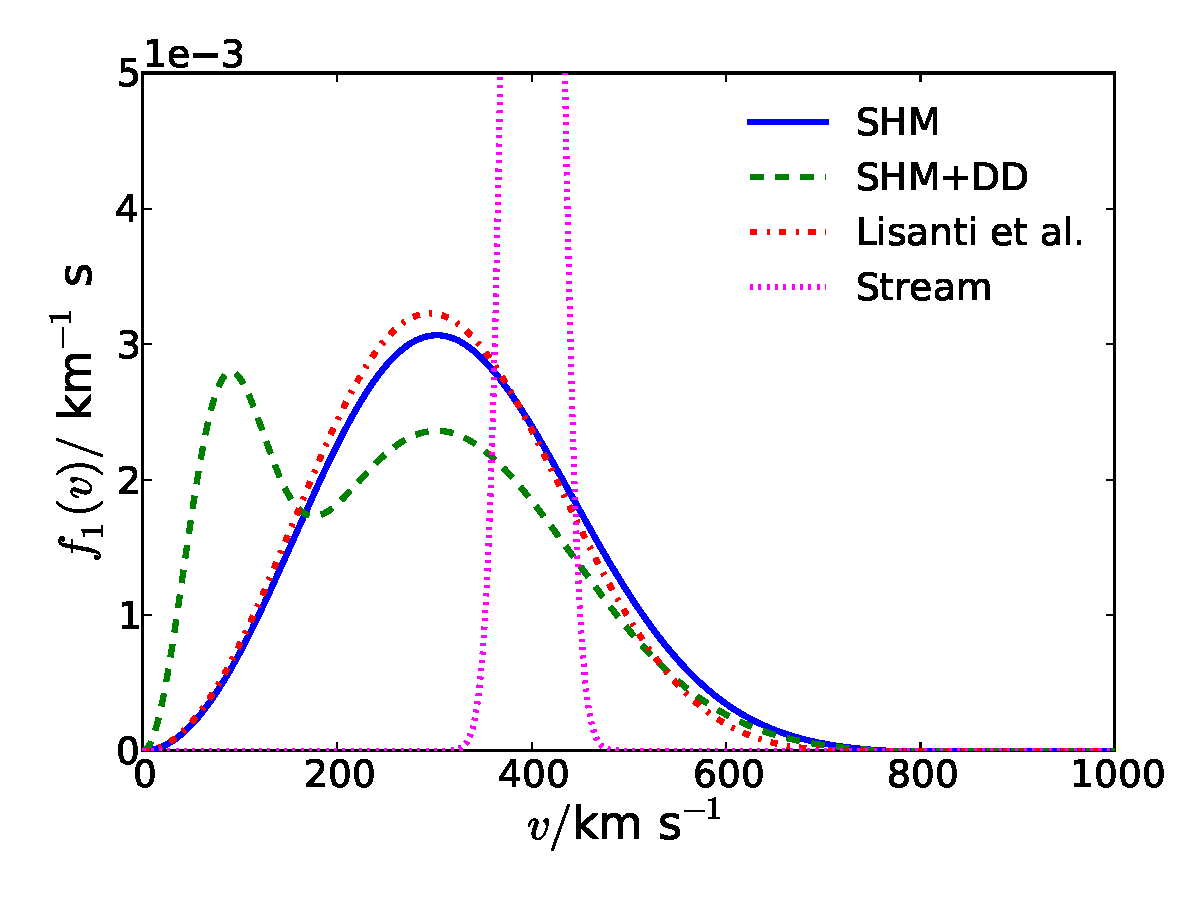
\includegraphics[width=\textwidth]{SpeedDistributions.pdf}
  \caption[Examples of dark matter speed distributions]{\note{Need actual caption - also, redo this plot.}}
  \label{fig:DD:SpeedDists}
\end{figure}

A first step is to extend the SHM to incorporate uncertainties in $v_\textrm{lag}$, $\sigma_v$ and $v_\textrm{esc}$ into reconstructions. Strigari and Trotta \cite{Strigari:2009} introduce a simple model of the Milky Way mass distribution, from which SHM velocity parameters can be derived. They then use projected stellar kinematics and direct detection data to fit both the model parameters and the dark matter properties. A more direct approach is to directly fit the SHM velocity parameters, incorporating their uncertainties into the fitting likelihood. This method has been considered by Peter \cite{Peter:2010}, and is typically used as a simple model of astrophysical uncertainties (especially in studies which focus on other aspects of direct detection, e.g.\ Ref.~\cite{Arina:2013}). These methods allow bias in the reconstructed WIMP parameters to be eliminated when the underlying speed distribution is indeed in the SHM form. However, as shown by Peter \cite{Peter:2011}, these methods fail when the distribution function differs from the standard Maxwellian case.

There have also been attempts to incorporate and fit more realistic distribution functions. Pato et al. \cite{Pato:2011} incorporate astrophysical uncertainties by using the distribution function of Lisanti et al. \cite{Lisanti:2010} and fitting the various shape parameters associated with it. In a more recent paper, Pato et al. \cite{Pato:2013} use projected direct detection data to fit a model of the Milky Way mass distribution, from which they derive a self-consistent distribution function (SCDF) using Eddington's formula. This means that the resulting speed distribution will be consistent with the underlying potentials of the galaxy's bulge, disk and dark matter, incorporating a broader range of shapes than the SHM alone. However, as the authors point out, velocity distributions from cosmological N-body simulations differ significantly from those expected from Eddington's formula. As with the Standard Halo Model, fitting a realistically-motivated distribution function is likely to result in biased reconstructions if the true distribution deviates significantly from the functional form used for fitting.

Methods which make no assumptions about the functional form of the speed distribution have had mixed success. Drees and Shan \cite{Drees:2007, Drees:2008} developed a method for estimating the WIMP mass by calculating moments of the speed distribution. However, this method still introduces a bias into the reconstructed WIMP mass and performs more poorly for heavier WIMPs and when finite energy thresholds are considered. An empirical ansatz for the speed distribution has also been suggested, specifically dividing the WIMP speed into a series of bins, with the distribution being constant within each bin \cite{Peter:2011}. \note{We will discuss this method in more detail in a later chapter...} However, both of these still result in a significant bias in the reconstructed mass and cross section. A recent proposal by Feldstein and Kahlhoefer \cite{Feldstein:2014} is to fit the velocity \textit{integral} rather than the speed distribution. This proposal is the most promising so far and appears to give an unbiased reconstruction of the mass, though reconstructing the speed distribution itself remains problematic. \note{This is shit - I need to say something more concrete about these...}

Finally, a method for analysing existing data has been developed by various authors \cite{Fox:2011b,Frandsen:2012, Gondolo:2012}. At a given mass, a given experiment is sensitive only to speeds in a fixed range, set by $v_\textrm{min}(E_\textrm{min})$ and $v_\textrm{min}(E_\textrm{max})$. By considering only the range of speeds where two or more experiments overlap, one can ensure that the astrophysical contribution to both experiments is equal. This method has typically been used to assess the compatibility of different data sets and to set more robust limits on the WIMP interaction cross sections. Recently it has also been extended to accomodate more general forms for the WIMP interactions \cite{DelNobile:2013}. \note{Again, be more specific - actually read these papers and put in some more detail - if it has to spill over into another chapter then fine... - Not sure, which is the McCabe one...}

\note{Need to spend lots more time on this section - less time on other sections... - maybe send some of the detector stuff to the first chapter...or some of this stuff to a later chapter...}

\note{May even be able to reconstruct f(v) itself - why is that good?}

\note{Masses and which bits are probed by which...}
\section{Conclusion}

We have discussed the dark matter direct detection formalism, focussing on the contribution from scalar and axial-vector contact interactions. The non-relativistic speeds involved means that the event rate can be divided into a spin-dependent and spin-independent contribution. A number of sophisticated experiments have been and continue to be developed which should allow these rare nuclear recoils to be detected. The use of different channels such as scintillation, ionisation and phonons not only allows the energy of these events to be measured but also allows discrimination against electronic recoils which can act as a significant background.

Tentative hints of a signal from the DAMA/LIBRA, CRESST-II and CoGeNT experiments have been interpreted as evidence for a WIMP with mass $m_\chi \sim 10 \GeV$ and cross section $\sigma_{SI} \sim 10^{-41} \cmsq$. However, null results from XENON, CDMS and other experiments are in tensions with this claimed signal. The origin of this discrepancy may lie in unidentified backgrounds or in an unconventional model for DM; corroboration from indirect and collider experiments may be needed before such a signal can be confirmed. 

Finally, there are a number of uncertainties associated with calculating direct detection event rates and therefore with interpreting data from these experiments. Nuclear uncertainties are typically more important for SD rate than for the SI, though the method of Cerde\~{n}o \etal may be able to reduce the impact of such uncertainties. Particle physics uncertainties are significant, though the standard contact operator approach should be a good first approximation and effective field theories extending beyond this standard approach are being developed. Uncertainties in the \textit{number} of dark matter particles, embodied in the local DM density $\rho_0$, lead to a factor of roughly 2 uncertainty in the total direct detection rate. 

In contrast, uncertainties in the speed distribution of dark matter are poorly controlled. Theoretical and computational considerations indicate that the benchmark assumption - the SHM - is not a good description of the WIMP distribution and while a large number of alternatives are available, it is unclear which, if any, of these may be correct. Attempts to treat the speed distribution more generally in data analysis have had mixed success, either leading to a biased reconstruction of the WIMP parameters or requiring additional assumptions or information about the WIMP, such as its mass. The wide range of possibilities for $f(v)$, as well as the consequences for misinterpreting future data, indicate that a more generalised approach is required.



%\chapter{Parameter Reconstruction}
\label{ch:ParamRecon}

\section{Introduction}

A common problem in physics is attempting to reconstruct the parameters of a model from a set of data. Stated more precisely, this is an attempt to answer the following question: given a set of data $\mathcal{D}$, what is the probability of a given set of model parameters $\boldsymbol\theta$ being the true, underlying parameters? But how do we interpret this question and what do we mean by the `probability' of a given set of parameters?

In general, there are two approaches to parameter estimation. In \textit{frequentist} inference, there is only a single, fixed set of true values for the model parameters $\boldsymbol\theta$. We imagine that the experiment (which produced the data $\mathcal{D}$) can be repeated a large number of times, giving independent results each time. The `probability' associated with each set of parameters $\boldsymbol\theta$ is a measure of how frequently our experiment would produce data which looked similar to $\mathcal{D}$ if $\boldsymbol\theta$ is the true value. In a frequentist framework, the true model parameters are fixed but unknown and we make statements about how confident we are that these true parameters lie in a particular range.

An alternative approach is \textit{Bayesian} inference. The true parameter value is treated as a random variable and we use Bayes' theorem to determine its probability distribution from the data:
\begin{equation}
P(\boldsymbol\theta|\mathcal{D}) = P(\boldsymbol\theta) \frac{P(\mathcal{D}|\boldsymbol\theta)}{P(\mathcal{D})}\,.
\end{equation}
In doing so, we need to know $P(\boldsymbol\theta)$, known as the prior on the model parameters. This is a measure of our beliefs about the true value of $\boldsymbol\theta$ and must be put in `by hand'. In a Bayesian framework, we combine the data with information about our prior expectations to make statements about the probability of $\boldsymbol\theta$ having a particular value.

These two approaches have different strengths and weaknesses, as we shall explore, and have both been applied to the problem of parameter exploration in physics. In this chapter, we will discuss how both frequentist and Bayesian statistics are used to make parameter estimates and measure the degree of certainty in these estimates. We will describe several methods which are used to explore parameter spaces and therefore make parameter inferences. Finally, we will outline how to calculate the likelihood $\mathcal{L}$ - the probability of obtaining a particular set of data given some underlying model parameters - which is at the core of both the frequentist and Bayesian approaches.

%Plan for this chapter:
%-`Shape of a parameter space' - define the likelihood and the posterior distribution (and marginalisation/profiling)
%-`Estimates' - what do we do for point estimates and spread estimates
%-`Methods' - MCMC and Nested Sampling
%-`Likelihood examples' - some likelihoods, such as poisson and extended (so that I don't have to do them later)


\section{Frequentist statistics}

%\subsection{Likelihoods}

In frequentist statistics, the most important quantity to consider is the \textit{likelihood} of a given point in parameter space, $\mathcal{L}(\boldsymbol\theta)$, defined as the probability of obtaining the data $\mathcal{D}$, assuming that $\boldsymbol\theta$ is the true parameter value. The likelihood often takes a very small value (because the probability of obtaining a particular data set out of all possible data sets is typically very small), and so it is convenient to work with the log-likelihood $l(\boldtheta) = \log(\mathcal{L}(\boldtheta))$. The absolute value of $\mathcal{L}(\boldsymbol\theta)$ carries no significance. However, the likelihood value of a particular point, relative to another, can be interpreted as a measure of the relative goodness of fit of the points. While the likelihood is not a probability distribution, in the limit of a large number of samples $l(\boldtheta)$ follows a $\chi^2$ distribution (as we shall discuss shortly) and therefore can have a probabilistic interpretation.

Often, we may not be interested in all of the parameters of $\boldtheta$. For example, we may partition the parameters into parameters of interests $\boldpsi$ and so-called nuisance parameters $\boldphi$: $\boldtheta = (\boldpsi, \boldphi)$. These nuisance parameters may be parameters which we are not directly interested in, but which must be included in the analysis to account for all the relevant uncertainties. We often want to reduce the dimensionality of $\boldtheta$ to consider only how the likelihood varies as a function of $\boldpsi$. 

One method of doing this is by maximizing the full likelihood function over the nuisance parameters:
\begin{equation}
\label{eq:parameter:profilelikelihood}
\mathcal{L}_p(\boldsymbol{\psi}) = \max_{\boldsymbol{\phi}} \mathcal{L}(\boldsymbol{\psi},\boldsymbol{\phi})\,.
\end{equation}
That is, for each value of $\boldpsi$, we select the maximum value of $\mathcal{L}$ obtained from all possible values of $\boldphi$. This projection onto the subset of parameters $\boldpsi$ is referred to as the profile likelihood.

An alternative method of reducing the dimensionality of the full parameter space is to calculate the mean likelihood:
\begin{equation}
\label{eq:parameter:meanlikelihood}
\mathcal{L}_m(\boldsymbol{\psi}) = \frac{\int \mathcal{L}(\boldpsi, \boldphi) \, \mathrm{d}\boldphi}{\int \, \mathrm{d}\boldphi}\,.
\end{equation}
The mean likelihood allows us to take into account the structure of the likelihood function in the nuisance directions. The profile likelihood simply selects the largest likelihood value at each value of $\boldpsi$, even if this value is only realised over a small range of values in $\boldphi$. By comparison, the mean likelihood receives a greater contribution from wide ranges of $\boldphi$ which have a moderate likelihood value.

\subsection{Parameter estimates}
\label{sec:ParamRecon:freqparams}
In frequentist statistics, the point estimate of a parameter is relatively unambiguous. This point estimate is given by the best fit point, or maximum likelihood estimate (MLE), $\hat(\boldtheta)$, such that:
\begin{equation}
\textrm{max}\mathcal{L}(\boldtheta) = \mathcal{L}(\hat{\boldtheta})\,.
\end{equation}
This estimate is the same whether we use the full likelihood or the profile likelihood, while using the mean likelihood may lead to a different value. In parameter inference, it is useful to consider the relative log-likelihood $l_r$:
\begin{equation}
l_r(\boldtheta) = -\log\left(\frac{\mathcal{L}(\boldtheta)}{\mathcal{L}(\hat{\boldtheta}}\right)\,.
\end{equation}
The logarithm is a monotonically increasing function and therefore the maximum in the likelihood and the minimum in the relative log-likelihood are obtained for the same parameter values $\hat{\boldtheta}$. According to Wilks' theorem \cite{Wilks:1938}, the $l_r$ is asympototically $\chi^2$-distributed as the number of samples $N$ increases,

\begin{equation}
-2l_r \sim \chi^2_k\,,
\end{equation}
where the number of degrees of freedom $k$ is equal to the dimensionality of the space $\boldpsi = \left(\psi_1,...,\psi_k\right)$. \note{Check minus signs etc...-everywhere} This asymptotic behaviour applies equally well for the full likelihood and the profile likelihood and allows us to construct confidence intervals. We construct a $p\%$ interval from all values of $\boldpsi$ for which 
\begin{equation}
l_r \geq \frac{1}{2} F^{-1}(p\%;k)\,,
\end{equation}
where $F^{-1}(p\%;k)$ is the inverse cumulative distribution of a $\chi^2$ distribution with $k$ degrees of freedom. That is we reject all parameter values for which $l_r$ exceeds the $p^\textrm{th}$ percentile of the $\chi^2_k$ distribution. This is essentially a goodness-of-fit test to determine, assuming that $\hat{\boldtheta}$ is the true parameter value, which values of $\boldtheta$ would not be rejected at the $p\%$ level. \note{Check this carefully...} Equivalently, in terms of the likelihood, we include values of $\boldtheta$ for which
\begin{equation}
\mathcal{L}(\boldtheta) \geq \exp\left(-\frac{1}{2} F^{-1}(p\%;k)\right) \mathcal{L}(\hat{\boldtheta})\,.
\end{equation}
We illustrate this methodology in Fig.~\ref{fig:parameter:likelihood}. 

\begin{figure}[t]
\centering
  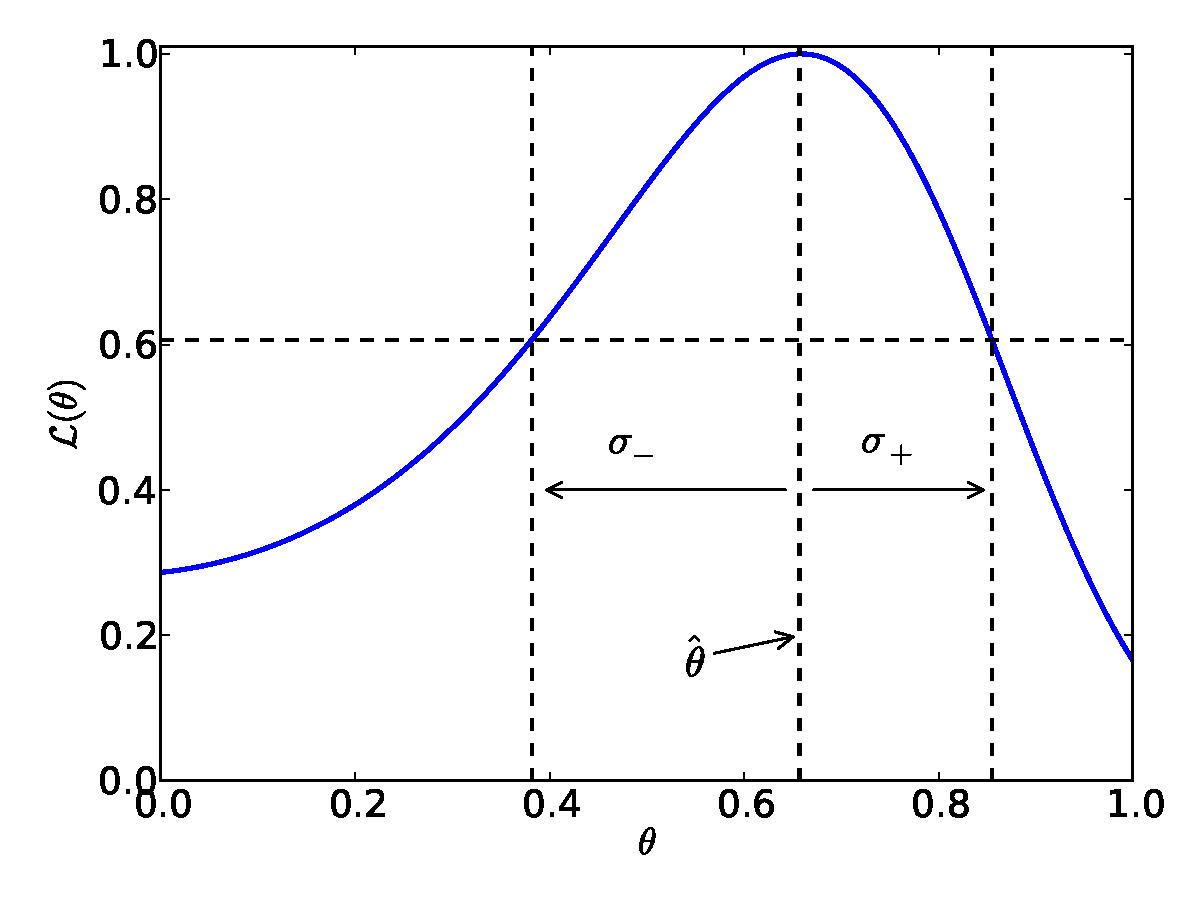
\includegraphics[width=0.8\textwidth]{ParamRecon/Likelihood.pdf}
  \caption[Likelihood-based parameter inference]{Illustration of likelihood-based parameter inference. The point estimate for the parameter $\theta$ is given by the best fit point $\hat{\theta}$. The 68\% confidence interval is given by $\theta \in [\hat{\theta} - \sigma_-, \hat{\theta} + \sigma_+]$.}
  \label{fig:parameter:likelihood}
\end{figure}

\section{Bayesian statistics}

In bayesian statistics, we wish to obtain the \textit{posterior} probability distribution $\mathcal{P}(\boldtheta) = P(\boldsymbol\theta|\mathcal{D})$. This is obtained from Bayes' theorem:
\begin{equation}
\mathcal{P}(\boldtheta) = P(\boldsymbol\theta|\mathcal{D}) = P(\boldsymbol\theta) \frac{P(\mathcal{D}|\boldsymbol\theta)}{P(\mathcal{D})}\,.
\end{equation}
Here $P(\mathcal{D})$ is the probability of obtaining the data $\mathcal{D}$. However, this does not depend on the theoretical parameters $\boldtheta$ and we can therefore take it as an overall normalising factor for the probability distribution. The likelihood enters into the Bayesian framework as probability of the data given the model parameters $P(\mathcal{D}|\boldsymbol\theta) = \mathcal{L}(\bold\theta)$. Finally, the prior $P(\boldsymbol\theta)$ encodes our \textit{a priori} knowledge about the true value of $\boldtheta$. If the value of a parameter, say $\theta_1$, is known to be approximately $\theta_1 = \hat{\theta}_1 \pm \sigma_\theta$, we may choose a Gaussian prior to reflect this:
\begin{equation}
P(\theta_1) \propto \exp\left(-\frac{(\theta_1 - \hat{\theta}_1)^2}{2\sigma_\theta^2}\right)\,.
\end{equation}
Alternatively, we may have a very limited knowledge of $\theta_1$ and may choose a linear-flat or log-flat prior over some range of values: $P(\theta_1) \propto 1$ or $P(\log(\theta_1)) \propto 1$. In the case of a linear-flat prior, $\mathcal{P}(\boldtheta) = \mathcal{L}(\theta)$ and the Bayesian and frequentist frameworks coincide. In contrast to the likelihood, the posterior distribution is considered a probability distribution, even in the case of small numbers of samples.

As in the frequentist case, we may wish to reduce the dimensionality of the parameter space to include only those parameters of interest $\boldpsi$. When dealing with the posterior probability, this is typically done by marginalisation. The marginalised posterior $\mathcal{P}_m$ is obtained by integrating over the nuisance parameters:

\begin{equation}
\mathcal{P}_m(\boldpsi) = \int \mathcal{P}(\boldpsi, \boldphi) \, \textrm{d}\boldphi\,.
\end{equation}
Just as $\mathcal{P}$ is a probability distribution function for the parameters $\boldtheta$, $\mathcal{P}_m$ is a probability distribution function for the parameters of interest $\boldpsi$ - specifically, the marginalised probability distribution.

\subsection{Parameter estimates}

In contrast to the frequentist case, there are several possibilities for a point parameter estimate \note{look up the qualities of each (mode/mean/median)}. Because $\mathcal{P}$ is a probability distribution, it can be described by several location parameters:

\begin{description}
\item[Mode] - the mode of the probability distribution is the value of $\boldtheta$ which maximises $\mathcal{P}$. This is also known as the maximum a posteriori (MAP) estimate and can be viewed as analogous to the maximum likelihood estimator.
\item[Median] - the median value of the parameter $\theta$ satisfies
\begin{equation}
\int_{-\infty}^{\theta_\textrm{median}} \mathcal{P}(\theta) \, \mathrm{d}\theta = \frac{1}{2}\,.
\end{equation}
This means that there is as much probability density below $\theta_\textrm{median}$ as above.
\item[Mean] - the mean value $\langle \theta \rangle$ is given by 
\begin{equation}
\langle \theta \rangle = \int \theta \mathcal{P}(\theta) \, \mathrm{d}\theta\,.
\end{equation}
\end{description}
Each of these will behave differently for different posterior probability distributions. The MAP estimate indicates where the greatest probability density is and may be useful when the posterior is sharpy peaked. The mean and median better reflect the global properties of the posterior probability, but may be misleading if the distribution is multimodal. 

\todo{Talk about multimodality}
\todo{Do a comparison of frequentist and bayesian - when do they coincide?}

We also wish to make statements about the possible range of values for parameters. In a Bayesian framework, we define the p\% \textit{credible} interval $\mathcal{C}_{p\%}$, defined such that it encloses p\% of the probability. Again, there are several possibilities for how to define $\mathcal{C}_{p\%} = [\mathcal{C}_{p\%}^\textrm{min} \mathcal{C}_{p\%}^\textrm{max}]$, such as:
\begin{description}
\item[Central interval] - the interval which has the mean as its central value.
\item[Equal tails interval] - the total probability below the interval is the same as above the interval,
\begin{equation}
\int_{-\infty}^{\mathcal{C}_{p\%}^\textrm{min}} \mathcal{P}(\theta) \, \mathrm{d}\theta = \int_{\mathcal{C}_{p\%}^\textrm{max}}^{\infty} \mathcal{P}(\theta) \, \mathrm{d}\theta\,.
\end{equation}
\item[Highest density interval] - the interval defined by all values $\mathcal{P}(\theta) \geq \gamma$, where $\gamma$ is defined by
\begin{equation}
\int_{\mathcal{P}(\theta \geq \gamma)} \mathcal{P}(\theta) \, \mathrm{d}\theta = p\%\,.
\end{equation}
\end{description}
Again, when we specify a credible interval, we must specify which definition we are using. These definitions can also be extended simply to the case where the parameter space of interest has a higher dimension. In Fig.~\ref{fig:parameter:PDF}, we illustrate the MAP estimate and mean for a hypothetical posterior distribution. We also show the 95\% credible interval obtained using the equal tails method.

\begin{figure}[t]
\centering
  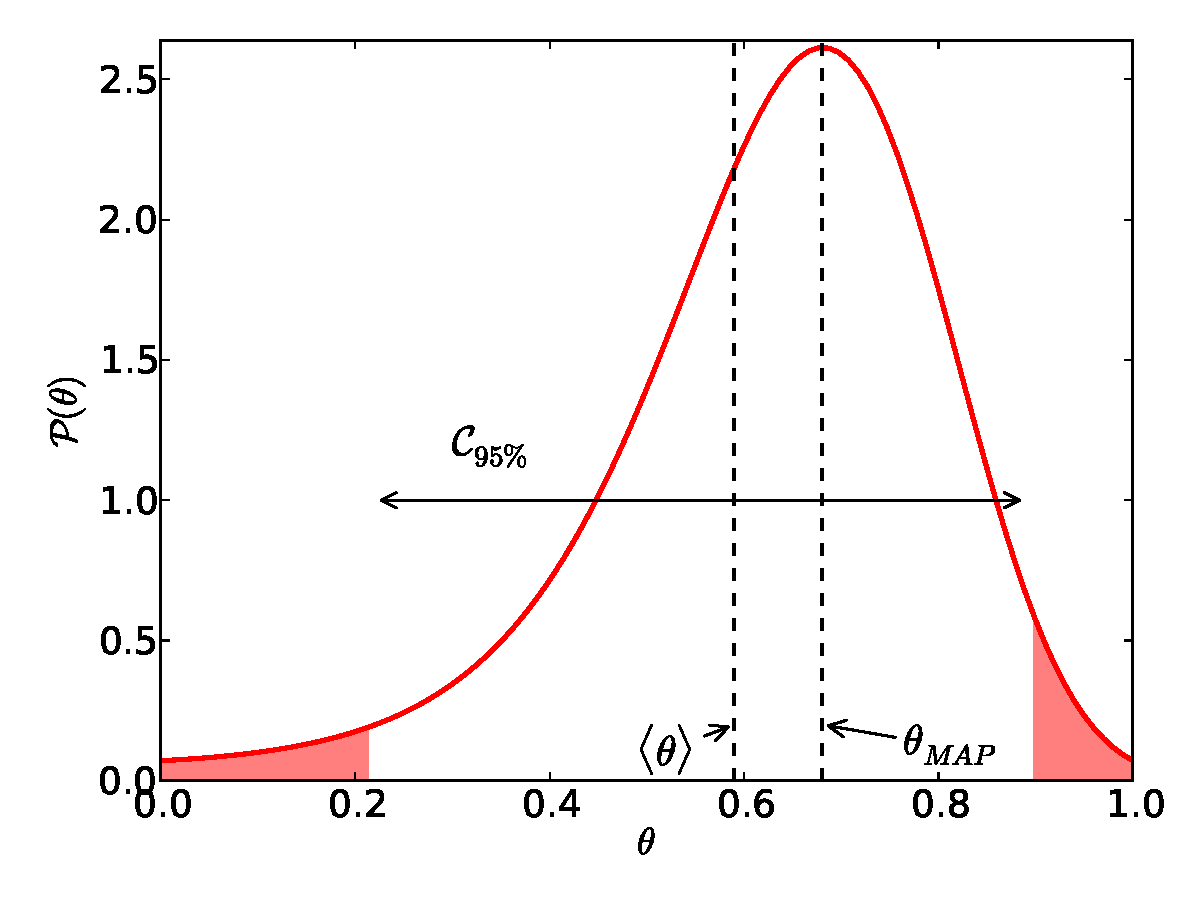
\includegraphics[width=0.8\textwidth]{ParamRecon/PDF.pdf}
  \caption[Posterior-based parameter inference]{Illustration of posterior-based parameter inference. We show the difference between the MAP and mean parameter estimates. We also show one possible 95\% credible interval - the probability in the shaded tails is equal.}
  \label{fig:parameter:likelihood}
\end{figure}


\section{Exploring the parameter space}

So far we have considered how, given $\mathcal{L}(\boldtheta)$ or $\mathcal{P}(\boldtheta)$, we can make parameter inferences about $\boldtheta$. However, we have not so far considered how we can evaluate these functions. We do not typically know \textit{a priori} where $\mathcal{L}(\boldtheta)$ or $\mathcal{P}(\boldtheta)$ are maximised or what shape they have. In this section, we will briefly discuss two methodologies for mapping out these functions: Markov Chain Monte Carlo and Nested Sampling.

\subsection{Markov chain monte carlo}


In the Markov chain monte carlo (MCMC) method \cite{Lewis:2009} \note{Need original citations as well}, we generate a chain of points in the parameter space $\left\{\boldtheta_i\right\}$. A new point $\boldtheta_{j+1}$ in the chain is generated from the current point $\boldtheta_{j}$ by picking from some proposal distribution $P(\boldtheta_{j}; \boldtheta_{j+1})$. Under the Metropolis-Hastings algorithm \cite{Metropolis:1953}, the new point is accepted with probability
\begin{equation}
\textrm{min}\left\{1, \frac{\mathcal{L}(\bold\theta_{j+1})Pr(\bold\theta_{j+1})}{\mathcal{L}(\bold\theta_{j})Pr(\bold\theta_{j})} \right\}\,,
\end{equation}
as long as the proposal distribution is symmetric. Over a large number of points, the chain should converge and eventually the number density of chain positions should be proportional to the posterior \(n(\boldtheta) \propto \mathcal{P}(\boldtheta)\). In addition, we will also have the value of the likelihood $\mathcal{L}(\boldtheta)$ evaluated at all of the points in the chain.

Care must be taken to ensure that the chain has converged before the results can be interpreted. Typically some initial set of points is discarded as `burn-in', after which the chain is deemed to have converged. However, it is often unclear when convergence has been reached. Moreover, each chain position will dependent slighly on the previous position. However, we want to obtain independent samples from the posterior distribution. Therefore, the chain is typically thinned (by some factor of order 25-50) \cite{Lewis:2002}, with only some of the positions being retained. Finally, we must select how many positions we want to obtain in the chain before we stop the random walk, in the hopes that the chain has adequately explored the parameter space. \note{Talk about R-tests...?}

When $\mathcal{P}(\boldtheta)$ is multimodal, sharply peaked or has strong degeneracies among the parameters, exploration by the chain can be slow. It can be unclear whether convergence has been achieved, especially if the chain becomes trapped in one of the modes of the distribution. One way to improve the rate of convergence is to use high temperature MCMC \cite{Kirkpatrick:1983,Lewis:2009}. We employ a `heated' chain with temperature $T = 2$, meaning that we accept new points with probability
\begin{equation}
\textrm{min}\left\{1, \left(\frac{\mathcal{L}(\bold\theta_{j+1})Pr(\bold\theta_{j+1})}{\mathcal{L}(\bold\theta_{j})Pr(\bold\theta_{j})}\right)^{1/T} \right\}\,.
\end{equation}
We are now effectively sampling from a flatter posterior distribution, which allows a more rapid mixing and convergence of the chain. However, to achieve the same precision as in the $T=1$ case, we require a larger number of samples. The distribution of chain positions obtained at the higher temperature is then \(n_\textrm{T}(\boldtheta) \propto \mathcal{P}^{1/T}(\boldtheta)\). We recover the distribution of positions at \(T=1\) by `cooling' the chain:

\begin{equation}
n(\boldtheta) = n_\textrm{T}(\boldtheta) \left(\mathcal{P}(\boldtheta)\right)^{1 - 1/T}.
\end{equation}

\todo{Pros and cons? Good at finding the best fit?}

One popular, publicly available MCMC code is \textsc{CosmoMC} \cite{Lewis:2002}. This was developed in the context of cosmological parameter estimation, but can be used as a generic MCMC sampler. \note{Anything else...?} When the parameter space is of a high dimension or has a number of modes, MCMC methods may prove slow. Such methods also rely on a suitable choice of burn-in and thinning factors, as well as a determination of whether convergence has occurred. Next, we explore an alternative method for efficiently obtaining samples from the posterior distribution.

\subsection{Nested sampling}

The nested sampling method \cite{Skilling:2004} was originally proposed as a method of calculating the overall normalising factor which appears in Bayes' theorem, $P(\mathcal{D})$. However, it produces as a by-product samples from the posterior distribution and values of the likelihood function. In nested sampling, we take an initial sample of points (so-called `live' points) from the parameter space and evaluate the likelihood at each point. The live point with the lowest likelihood $\mathcal{L}_0$ is removed from the sample and replaced with another point sampled from the parameter space with $\mathcal{L}_i > \mathcal{L}_0$. Thus, the algorithm explores the prior in concentric shells of $\mathcal{L}$. Each new live point can be assigned a weight $w_i$, obtained from an estimate of change in prior volume between concentric shells. Finally, each point can then be assigned a posterior density

\begin{equation}
p_i = \frac{w_i \mathcal{L}_i}{\mathcal{Z}}\,.
\end{equation}
The Bayesian evidence $\mathcal{Z} \equiv P(\mathcal{D})$ is obtained by summing $\sum_i w_i \mathcal{L}_i$ and the algorithm continues until this is determined to some desired precision.

In order to continue, we must be able to select points from the prior subject to the hard constraint $\mathcal{L}_i > \mathcal{L}_0$. As the algorithm moves to higher values of $\mathcal{L}_0$, points with a higher likelihood than this tend to become localised in very small regions of the parameter space. In addition, if the likelihood is multimodal or has pronounced degeneracies, the sampling of points subject to this constraint becomes highly inefficient. The \textsc{MultiNest} algorithm \cite{Feroz:2007,Feroz:2008,Feroz:2014} uses multimodal, ellipsoidal nested sampling to improve performance. As $\mathcal{L}_0$ increases during the calculation,  \textsc{MultiNest} uses the current live points to approximate the isolikelihood contour by a series of ellipsoidal surfaces. New points are drawn only from within these ellipsoids, increasing the efficiency of the sampling but still ensuring that the constraint $\mathcal{L}_i > \mathcal{L}_0$ is satisfied. The algorithm can also accomodate multiple modes in the posterior which can be explored independently.

In utilising the MultiNest algorithm, we must decide how many live point to use $N_\textrm{live}$. This determines how closely the isolikelihood contours can be followed, how dense the posterior samples will be and, in the case where there are highly localised modes, how well explored the prior will be. We must also decide the tolerance of the algorithm \texttt{tol}. This determines the precision with which $\mathcal{Z}$ should be determined and therefore how high up the likelihood surface the algorithm should explore. Finally, we can introduce an efficiency \texttt{eff}, which is the desired sampling efficiency. In order to (attempt to) achieve this, the algorithm rescales the volume of the bounding ellipsoids to incorporate more or less of the prior volume, as desired. 

\todo{Model selection...? - Leave this until later...}

\todo{Could look at event generation...}

\section{Likelihood examples}

We have discussed how, given the likelihood and posterior, we can make parameter inferences. We have also explored methods by which these functions can be efficiently explored. Finally, we look at how to evaluate the likelihood for a given data set. 

The simplest signal which can be observed is a number of events $N_o$. We can calculate from the model parameters $\boldtheta$ the expected number of events $N_e$ following Sec.~\ref{}. The probability of obtaining the data given the model parameters is then given by the Poisson likelihood:

\begin{equation}
\mathcal{L}(N_o|N_e) = \frac{N_e^{N_0}}{N_0!}e^{-N_e}\,.
\end{equation}
We can extend this definition to incorporate data which has been divided into bins with $N_e^{(i)}$ events expected and $N_o^{(i)}$ observed in the $i^\textrm{th}$ bin:
\begin{equation}
\label{eq:ParamRecon:binnedL}
\mathcal{L}(\{N_o^{(i)}\}|\{N_e^{(i)}\}) = \prod_{i = 1,N_\textrm{bins}} \frac{(N_e^{(i)})^{N_o^{(i)}}}{(N_o^{(i)})!}e^{-N_e^{(i)}}\,.
\end{equation}
We can also consider the unbinned likelihood by taking the limit as the bin width tends to zero,
\begin{equation}
\label{eq:ParamRecon:unbinnedL}
\mathcal{L}(\mathcal{D}|\boldtheta) = \frac{N_e^{N_0}}{N_0!}e^{-N_e}\prod_{i = 1,N_e} P(E_i)\,,
\end{equation}
where $N_e$ and $N_o$ are the number of events expected and observed across the whole experiment. We have assumed here that each event has an associated measurement, the energy $E_i$, and we take the product over the normalised event rates:
\begin{equation}
P(E) = \dbd{R}{E_R}(E)\left[\int_0^{\infty} \dbd{R}{E_R}(E')\,\mathrm{d}E'\right]^{-1}\,.
\end{equation}

Finally, we may wish to include the effects of background in the analysis. Then, we must take into account the fact that we do not know whether a given even is due to the signal or background. It will derive from the signal with probability
\begin{equation}
f_S = \frac{N_\textrm{signal}}{N_\textrm{signal} + N_\textrm{background}}\,,
\end{equation}
and from the background with probability $f_{BG} = 1-f_S$. Thus, we obtain the full likelihood
\begin{equation}
\mathcal{L}(\mathcal{D}|\boldtheta) = \frac{N_e^{N_0}}{N_0!}e^{-N_e}\prod_{i = 1,N_e} \left(P_S(E_i)\right)^{f_S}  \left(P_{BG}(E_i)\right)^{f_{BG}} \,.
\end{equation}
Here, $N_e$ and $N_o$ are the total number of expected events including both signal and background. We must also take into account the normalised spectra of the signal $P_S(E)$ and the background $P_{BG}(E)$ seperately, multiplying the contributions of both.

\todo{What else do I need?}

\note{ASIMOV!!!}

\section{Conclusions}

In this chapter, we have described two frameworks for parameter inference - frequentist and Bayesian statistics. We have described various possibilities for point and spread estimates of parameters in both cases, as well as how these should be interpreted. While both methodologies present different viewpoints on the problem of parameter estimation, they can be used in a complementary fashion and can, in the case of flat priors, coincide.

The MCMC and MultiNest algorithms can be used to efficiently sample from both the likelihood and posterior distribution, even in the case of highly complicated parameter spaces with multiple modes or pronounced degeneracies. We have also detailed a number of relevant cases for the explicit form of the likelihood function in binned and unbinned scenarios.

These techniques are essential for the later work presented in this thesis. In attempting to parametrise the dark matter velocity distribution a large number of parameters are needed to capture a range of possible features. In addition to particle physics and experimental nuisance parameters, this leads to a large parameter space which is a challenge to explore. However, as we will show, these techniques allow us to make concrete and unbiased estimates of both particle physics and astrophysical parameters based on future data sets.


%%%Could do `reconstructing the WIMP mass' and `reconstructing the cross section'...

\chapter{Parametrising the dark matter momentum distribution}


\chapter{Parametrising the speed distribution}
\label{ch:Speed}

As we have explored in Chapter~\ref{ch:DD}, there are a number of uncertainties associated with calculating the direct detection event rate. These translate directly into uncertainties in the analysis of direct detection results, present and future. If these uncertainties are properly accounted for, they can provide a more realistic estimates of uncertainties on the WIMP cross sections \sigmapsi and \sigmapsd and WIMP mass \mchi. If, however, our assumptions do not reflect the underlying nuclear physics, particle physics or astrophysics of dark matter, this can lead to a bias in the WIMP parameters. Understanding these uncertainties and how to mitigate them is therefore of great importance.

The WIMP speed distribution $f(v)$ enters into the direct detection event rate as it influences both the typical flux of dark matter particles and the typical recoil energy imparted during a scattering event. Unfortunately, the typical flux and recoil energy are also strongly dependent on the WIMP mass \mchi. This leads to a strong degeneracy between \mchi and $f(v)$ and, as discussed in Sec.~\ref{sec:DD:astrophysics}, the possibility of significant bias in the reconstruction of the WIMP mass (see e.g. Ref~\cite{Peter:2011}). \note{Maybe move some of the DD background chapter stuff to here...} In Sec.~\ref{}, we revisit the problem of reconstructing the WIMP mass and how it can be influenced by poor assumptions about $f(v)$.

Because the speed distribution is so poorly constrained, an ideal goal would be to construct the most general parametrisation for $f(v)$ which can accommodate a wide range of possibilities for the true functional form. This approach has previously been explored by Peter \cite{Peter:2011}, who wrote down an empirical parametrisation for $f(v)$ as a series of constant bins in $v$. However, this still resulted in a bias in the reconstructed WIMP parameters. In Sec.~\ref{sec:Speed:binned}, we analyse in more detail the performance of this method and attempt to explain where this bias comes from.

In Sec.~\ref{sec:Speed:momentum}, we discuss a method analogous to that of Peter but for parametrising the WIMP \textit{momentum} distribution in terms of a series of constant bins. This transformation helps remove some of the degeneracy between the WIMP mass and distribution function and improves reconstructions of the mass compared to binning in $f(v)$. However, this method is not generally applicable and begins to fail for low mass WIMPs. 

%In Sec.~\ref{sec:Speed:poly}, we propose an alternative parametrisation. Instead of parametrising $f(v)$, we parametrise the logarithm of $f(v)$ as a series of polynomials. This permits the most general possible form from $f(v)$ satisfying the constraint $f(v) \geq 0$. We demonstrate the performance of this new method over a range of WIMP masses and over a range of underlying speed distributions and experimental parameters. We show that this method allows us to reconstruct the WIMP mass without bias, as well as allowing us to reconstruct information about the WIMP speed distribution itself. \note{What about doing some 1-D plots for $f(v)$ parameters, such as plotting $\langle v \rangle$ or similar...?}

Finally, we compare these different parametrisations in Sec.~\ref{sec:Speed:discussion} and discuss how they relate to alternative methods of accounting for astrophysical uncertainties in direct detection experiments. We will also discuss the weaknesses of the momentum parametrisation, highlighting where remaining work is needed. 

\section{Uncertainties in $f(v)$}
\label{sec:Speed:uncertainties}

Dark matter direct detection experiments simultaneously probe the WIMP speed distribution and WIMP mass. As described in Chapter~\ref{ch:DD}, the differential event rate relevant for direct detection experiments is

\begin{equation}
\dbd{R}{E_R} = \frac{\rho_0}{2 \mu_{\chi p}^2 m_x} \sigma_{SI}^p A^2 F_{SI}^2(E_R) \int_{v_\textrm{min}}^\infty \frac{f(v)}{v}\,\mathrm{d}v\,,
\end{equation}
where for simplicity we have assumed that the coupling to protons and neutrons is the same ($f_p \approx f_n$) and we consider only the spin-independent (SI) contribution to the rate. Not also is the SI contibution expected to dominate for heavy nuclei (due to the $A^2$ enhancement), but considering only a single contribution allows us to focus on the degeneracies between \mchi, \sigmapsi and $f(v)$. 

We have previously outlined in Chapter~\ref{ch:DD} that there are various possibilities for the form of the WIMP speed distribution and that poor assumptions about this form may lead to biased reconstructions of the WIMP parameters. This has been demonstrated, for example, by Peter \cite{Peter:2011}, who attempted to reconstruct the WIMP mass and SI cross section from mock data sets based on future direct detection experiments. In order to generate the data, an SHM distribution function with an additional contribution from a dark disk was assumed. However, the posterior distribution for \mchi and \sigmapsi was obtained assuming that $f(v)$ could be well described by a single Maxwell-Boltzmann (MB) distribution (with average speed and speed dispersion included as nuisance parameters). The resulting marginalised 68\% and 95\% contours for \mchi and \sigmapsi are shown in Fig.~\ref{fig:Speed:PeterRecon}, with the true parameter values given by the black crosses.

\begin{figure}[h]
  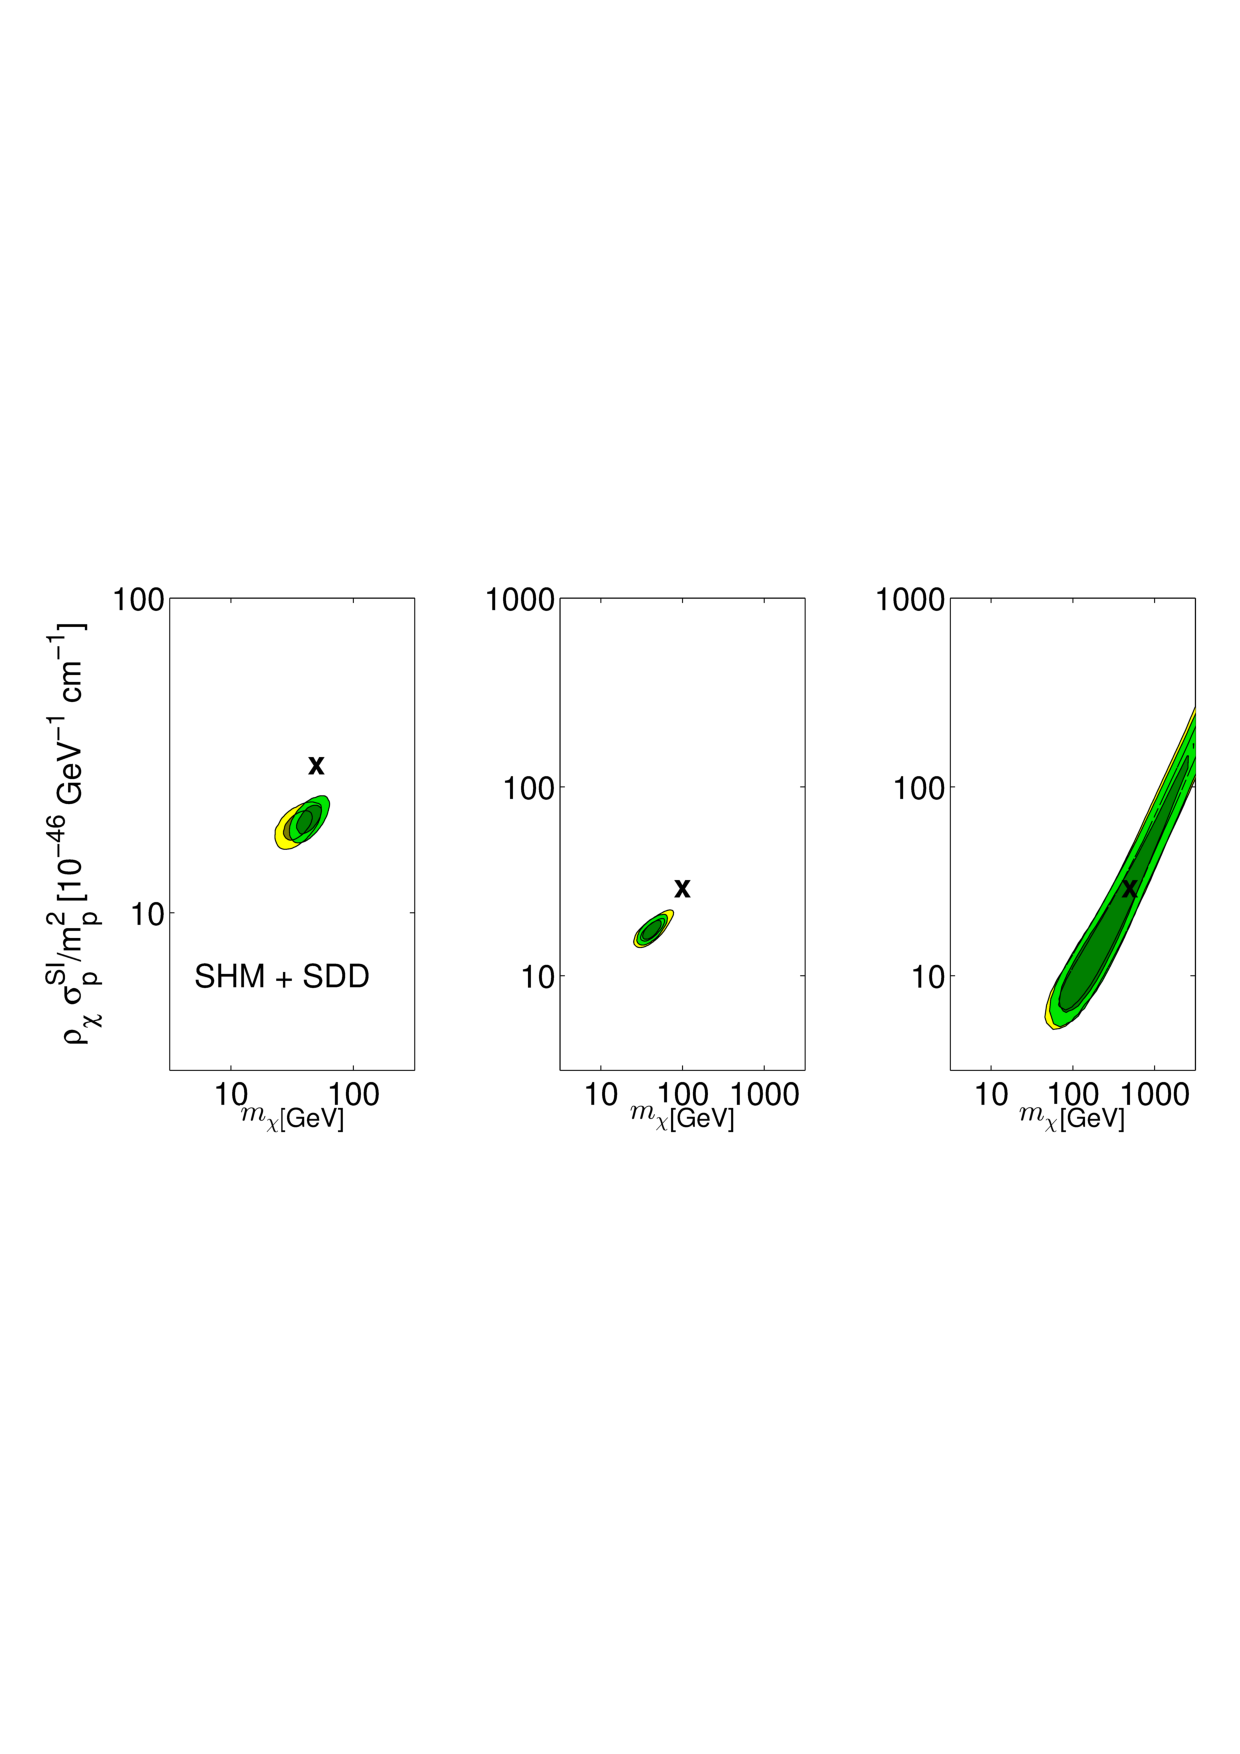
\includegraphics[trim={0cm 9cm 0cm 9cm},clip,width=\textwidth]{Speed/PeterRecon.pdf}
  \caption[Biased reconstruction of WIMP parameters]{\note{Need caption...} Reproduced from Ref.~\cite{Peter:2011}}
  \label{fig:Speed:PeterRecon}
\end{figure}

Even including some uncertainties in the shape of the MB speed distribution, there is still a clear bias in the reconstructed WIMP parameters. The MB speed distribution cannot reproduce the shape of the event spectrum closely and the WIMP mass and cross section move to different values to compensate and improve the fit. Not only is there a bias, but the resulting contours are relatively small. In this case, if we trust the ansatz of a MB distribution, we would mistakenly believe that we had reconstructed the WIMP parameters accurately with a high precision. Thus, there is a need for a more general approach which allows a broad range of speed distributions to be probed. We discuss the consequences of such an approach now. \todo{Improve flow...}

We can write the integral over the speed distribution as 
\begin{equation}
\label{eq:Speed:eta}
\eta(\vmin) \equiv \int_{\vmin}^\infty \frac{f(v)}{v}\,\mathrm{d}v\,, 
\end{equation}
where \vmin is given by
\begin{equation}
v_\textrm{min} = v_\textrm{min}(E_R, \mchi, m_N) = \sqrt{\frac{m_N E_R}{2 \mu_{\chi N}^2}}\,.
\end{equation}
If we treat $f(v)$ as a free function (subject to the condition that it be normalised to unity and everywhere positive), this is equivalent to treating $\eta(\vmin)$ as a free function (subject to the equivalent condition that $eta$ be a monotonically decreasing function of \vmin). This represents an entirely agnostic approach to $f(v)$, assuming that we know nothing at all about its functional form. Unfortunately, if we fix $m_N$, any change in the form of $\eta$ can be counteracted by a change in $\mchi$ (and a resulting change in \vmin) leading to the same spectral shape $\eta(E_R)$. This means that for a single experiment, the WIMP mass and $f(v)$ are exactly degenerate and we need multiple experiments to disentangle the two \cite{Drees:2008}. We will phrase this in more concrete terms later in Sec.~\ref{sec:Speed:momentum}.

Another consideration when parametrising $f(v)$ is the range of sensitivity of the experiments. Each experiment will have a window recoil energies to which it is sensitive $\left[\Emin, \Emax\right]$ (though the recoil detection efficiency may vary across this window). This means that for a given WIMP mass, each experiment will be sensitive only a range of WIMP speeds $\left[\vmin(\Emin), \vmin(\Emax)\right]$. WIMPs with speeds smaller than $\vmin(\Emin)$ do not contribute to the velocity integral defined in Eq.~\ref{eq:Speed:eta}. WIMPs with speeds above $\vmin(\Emax)$ can contribute to the overall spectrum, but they contribute only a constant, additive rate; the experiment is not sensitive to the \textit{shape} of the speed distribution above this maximum speed. Thus, each experiment has a range of speeds to which it is sensitive. If we wish to probe the shape of $f(v)$, these ranges must have some overlap between the different experiments. Otherwise, the $f(v)$ can be varied independently across each speed range and the degeneracy between \mchi and $f(v)$ remains. \todo{Insert and explain plot...}

In order to get a handle on $f(v)$ and therefore the WIMP mass we therefore need several direct detection experiments, which use different target materials but which probe overlapping WIMP speeds. However, we must come up with a way of writing our general function $f(v)$ which allows us to reconstruct it by fitting to the data. Such a parametrisation should correspond to a physical distribution function; it should be normalised and should be everywhere positive. We should try to write down a parametrisation which spans a wide range of underlying distribution functions and which does not introduce any additional bias into attempts to reconstruct the WIMP parameters. For this reason, it is necessary to carefully test any proposed parametrisation. We now explore in more detail several proposal for what such a general parametrisation should look like.

\todo{Talk about the transformation from the Galactic to Earth frame...}

\section{Binned speed distribution}

Peter proposed using an empirical speed distribution in the form of series of bins in speed $v$ in order to fit to data. Explicitly, we write the WIMP speed distribution (in the Earth frame), as a series of \(N\) bins of constant value, with bin edges \(\{ \tilde{v}_i\}\): \note{This is the directionally averaged velocity distribution...}

\begin{equation}
\label{eq:Speed:binned}
f(v) = \sum_{i = 1}^N g_i \, W(v;\tilde{v}_i,\Delta v) \,,
\end{equation}
where the top-hat function, W, is defined as:

\begin{equation}
W(v;\tilde{v}_i,\Delta v) =
\begin{cases}
   1 &  v \in [\tilde{v}_i,\tilde{v}_i+\Delta v] \\
   0  & \text{otherwise}
  \end{cases} \,.
\end{equation}
We must choose a maximum speed $v_\textrm{max} = N\Delta v$ up to which we parametrise. Beyond this speed, we set $f(v)$ to zero, so we should choose a conservative value which does not risk truncating the speed distribution prematurely. Based on the results of the RAVE surveys \cite{RAVE:2007, RAVE:2014}, the Galactic escape speed is estimated to be $\vesc < 587$ at the 90\% confidence level. Assuming a local circular speed of $v_c \sim 220 \kms$ \cite{Kerr:1986,Feast:1997}, this means that in the Earth frame, particles with speeds significantly higher than $v_c + \vesc \sim 800 \kms$ should not be gravitationally bound. This is consistent with results for the local escape speed obtained in N-body simulations \cite{Kuhlen:2010}. We therefore choose a value $v_\textrm{max} = 1000 \kms$ as a conservative upper limit for the parametrisation.

The form for the distribution function given in Eq.~\ref{eq:Speed:binned} is the directionally-averaged WIMP velocity distribution, $f(v)$. The WIMP \textit{speed} distribution is then given by

\begin{equation}
\label{eq:Speed:binned2}
f_1(v) = \sum_{i = 1}^N g_i v^2\, W(v;\tilde{v}_i,\Delta v) \,.
\end{equation}
Imposing normalisation of the speed distribution, we obtain the following constraint on the \(\{g_i\}\):
\begin{equation}
\label{eq:Speed:Normg}
\sum_{i = 1}^N g_i \, \left[(\tilde{v}_i + \Delta v)^3 - \tilde{v}_i^3\right]/3 = 1 \,.
\end{equation}
For notational convenience, we also define
\begin{equation}
\hat{g}_i = g_i \, \left[(\tilde{v}_i + \Delta v)^3 - \tilde{v}_i^3\right]/3 \,,
\end{equation}
such that the normalisation condition becomes
\begin{equation}
\label{eq:Speed:ghat}
\sum_{i = 1}^N \hat{g}_i = 1.
\end{equation}
\todo{Distinguish between f1 and f...}

\todo{Earth frame}

We illustrate the form of this binned distribution for $f(v)$ in Fig.~\ref{fig:Speed:BinApprox}. We show the Standard Halo Model in the Earth frame (blue line) as well as the binned approximation to the SHM (red line). This approximation is obtained by integrating the WIMP speed distribution over each of the bins:

\begin{equation}
\label{eq:Speed:gapprox}
\hat{g}_i^\textrm{approx} = \int_{\tilde{v}_i}^{\tilde{v}_i + \Delta v} f_1^{\textrm{SHM}}(v) \, \mathrm{d}v\,.
\end{equation}
This allows us to examine how closely the binned parametrisation can be used to approximate the SHM. However, in a realistic scenario, these bin parameters $\left\{\hat{g}_i\right\}$ would form part of the parameter space, along with \mchi and \sigmapsi, which must be explored based on the data. \note{Also plot the approximate form for $\eta$ here!}

\begin{figure}[h]
\centering
  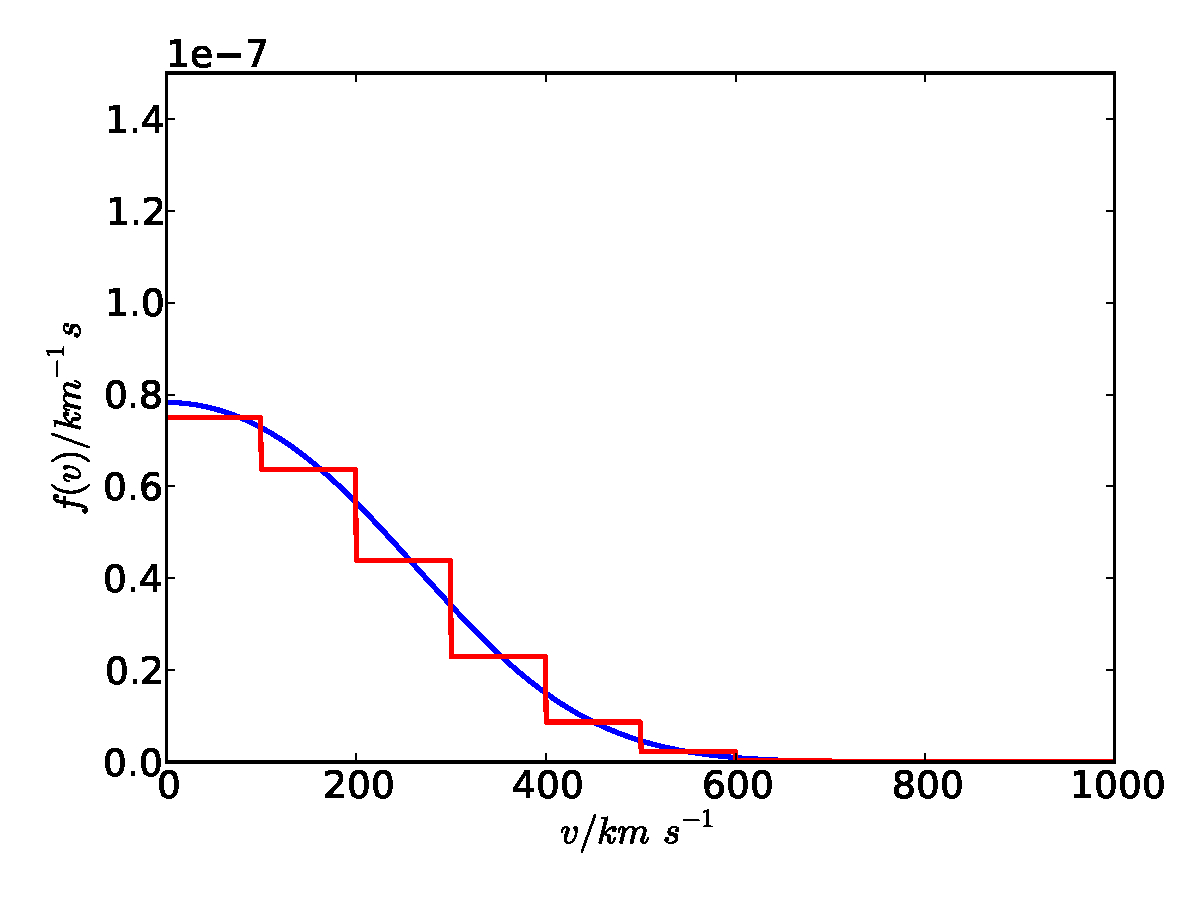
\includegraphics[width=0.75\textwidth]{Speed/BinnedApprox.pdf}
  \caption[Binned approximation to the SHM]{Binned approximation to the SHM in the Earth frame. The bin heights are obtained from Eq.~\ref{eq:Speed:gapprox}. We note that shown here is $f(v)$, the directionally-averaged velocity distribution. We must multiply by $v^2$ to obtain the speed distribution $f_1(v)$.}
  \label{fig:Speed:BinApprox}
\end{figure}

In Ref.~\cite{Peter:2011}, Peter found evidence that this method still lead to a bias in the reconstructed WIMP mass and cross section, despite the apparent generality of this binned distribution function. Here, we explore this method further. In particular, we consider a large number of realisations of data sets from hypothetical future experiments, assuming some fiducial benchmark model. We then attempt to reconstruct the WIMP mass for each realisation, allowing us to determine how the method performs statistically and whether the bias found by Peter is present in all data sets or only in a small number of Poissonian realisations.

\subsection{Benchmark Parameters and Experiments}
\label{sec:Speed:Experiments}
As noted in Sec.~\ref{sec:Speed:uncertainties}, it is impossible to estimate the WIMP mass from a single experiment if no assumptions are made about \(f(v)\), so we consider three next-generation detectors, modelled on experiments which are currently in development. Each experiment is characterised by a single (suitably averaged) target nucleus mass, \(m_N\), a total detector mass, \(m_\textrm{det}\), an effective exposure time, \(t_\textrm{exp}\), and a pair of energies, \(E_\textrm{min}\) and \(E_\textrm{max}\), which mark the extent of the signal region. We focus on a particular set of experimental parameters in order to provide a concrete example of how the WIMP parameters can be estimated accurately. Table \ref{tab:Speed:Expts} shows the experimental parameters used in this work, which are chosen to approximately match those used by Peter \cite{Peter:2011}.

\begin{table}[t]
  \begin{center}
    \begin{tabular}{lm{2cm}m{2.1cm}m{1.7cm}}
    \hline\hline
    & XENON1T \cite{Aprile:2009a} & SuperCDMS \cite{Bruch:2010} & WArP \cite{Szelc:2009} \\
\hline
Detector Target & Xe & Ge & Ar \\
Nuclear Mass, \(m_\textrm{N} / \textrm{amu}\) & 131 & 73 & 40 \\
Detector Mass, \(m_\textrm{det} / \textrm{kg} \) & 1000  & 100 & 1000 \\
Exposure Time, \(t_\textrm{exp} / \textrm{days} \) & 60.8  & 109.5 & 365\\
Energy Range, \(\left[E_\textrm{min},E_\textrm{max} \right] / \textrm{keV}\) & [2,30] & [10,100] & [30,130] \\
    \hline\hline
    \end{tabular}
  \end{center}
  \caption{Parameter values for the three mock experiments used in this work, chosen to closely match those used in Ref.\ \cite{Peter:2011}. The meanings of the experimental parameters are described in Sec.\ \ref{sec:Speed:Experiments}.}
\label{tab:Speed:Expts}
\end{table}
We assume perfect and uniform detection efficiency - that is, all signal events and no background events survive analysis cuts. We also assume perfect energy resolution. For a real experiment, these assumptions will almost certainly not hold, for example due to variations in the relative scintillation efficiency of Xenon \cite{Aprile:2009b}, but the results presented here should be viewed as a proof of principle in the ideal case.

\begin{figure}[t]
  \centering
  \includegraphics[width=0.75\textwidth]{Speed/AccessSpeeds_New.eps}
\caption{Range of accessible WIMP speeds for each of the three mock experiments: XENON1T-like (solid blue), SuperCDMS-like (dashed green) and WArP-like (dot-dashed red). Each pair of lines corresponds to the maximum and minimum accessible WIMP speeds for a given experiment. The outermost dotted red lines show the accessible speeds for the adjusted parametrisation range described in Sec.\ \ref{}.}
  \label{fig:Speed:Access}
\end{figure}

Figure \ref{fig:Speed:Access} shows the minimum and maximum accessible WIMP speeds for each experiment. All three experiments rapidly become insensitive to WIMPs with speeds less than \(\sim 1000 \kms\) as the WIMP mass drops below \(m_\chi \sim 10 \textrm{ GeV}\). This suggests that the experiments considered here generically have a low sensitivity to such light WIMPs, producing too few events for accurate parameter reconstruction. \note{So what...?}

For comparison with later methods, we consider here a single benchmark model: \(m_\chi = 50 \textrm{ GeV}\), $\sigmapsi = 10^{-44} \mathrm{cm}^2$ and the SHM. We assume a fixed value for the local DM density $\rho_0 = 0.3 \textrm{ GeV cm}^{-3}$. As will be explained in Sec.\ \ref{sec:MomentumMethod2}, the precise values of \sigmapsi and \(\rho_0\) are not particularly important due to the degeneracy between these two parameters. The total number of events from all three detectors combined typically ranges from around 300 to 600 for the different benchmark parameters which will be considered in this chapter. 

\subsection{Parameter reconstruction}
We generate 250 mock data sets using the experiments described above. We then use the Markov Chain Monte Carlo (MCMC) package CosmoMC \cite{} to make parameter inferences on the parameters $\mchi, \sigmapsi, \left\{\hat{g}_i\right\}$, where $\hat{g}_i$ are the bin parameters for a 5 bin speed distribution function. We sample the WIMP mass and cross-section logarithmically in the ranges \([10, 1000] \textrm{ GeV}\) and \([10, 10000] \times 10^{-47} \textrm{ cm}^2\) respectively, with log-flat priors on both. We sample the $\hat{g}_i$ linearly in the range $[0,1]$, subject to the normalisation constraint of Eq.~\cite{eq:Speed:ghat}. We perform the MCMC at a temperature $T=2$ to ensure adequate exploration of the parameter space.

In order to obtain an estimate of parameters, we use the mean likelihood, as described in Chapter~\ref{ch:ParamRecon}. We bin the parameter of interest and average the likelihood of all points within each bin. This mean likelihood is then smoothed on the width of the bins and the parameter value which maximises the mean likelihood is taken as a best estimate of the underlying parameter. In order to obtain parameter limits, we construct minimal credible intervals for the parameters of interest at the $p\%$ level. \note{This is all shite...Wait, am I actually using the marginalised PDF - yes, yes I am - rewrite!!! I'm using MAP! Why change?}

\subsection{Results}
Figure~\ref{fig:Speed_MassFit} shows the fitted values for the WIMP mass, \(m_\textrm{rec}\), obtained from 250 mock datasets. This distribution shows a peak around 45 GeV, as well as a significant number of datasets reconstructed at \(\sim 100 \textrm{ GeV}\). As pointed out by Ref.\ \cite{Strege:2012}, some mock datasets will not be representative of the underlying benchmark parameters, having more events at high energies than expected, for example. This can lead to `bad' reconstructions with a fitted WIMP mass higher than the benchmark value. Thus, the reconstructions near \(100 \textrm{ GeV}\) do not necessarily signify a failure of the reconstruction method.

 \begin{figure}[t]
\centering
  \includegraphics[width=0.75\textwidth]{Speed/Speed_MassFit.eps}
  \caption{WIMP masses reconstructed using the speed parametrisation method from 250 realisations. The benchmark speed distribution is the SHM. The true mass of 50 GeV is shown as a dashed vertical line.} 
  \label{fig:Speed:Speed_MassFit}
\end{figure}

However, a coverage study of 68\% and 95\% confidence intervals for this method shows significant under-coverage: \(36 \pm 3 \%\) coverage and \(63 \pm 3 \%\) coverage respectively for the two intervals. This indicates that while the mass reconstructions appear to be distributed close to the true value, the corresponding error estimates must be too small. \todo{Actually write the coverage section in Chapter 3 - or just get rid of chapter 3 all together...?}

We can also assess the performance of the method by calculating the `pull' statistic \(\Delta\) (see e.g.\ Ref.\ \cite{Pulls}),
\begin{equation}
\Delta = \frac{m_\textrm{rec} - m_\textrm{true}}{\sigma} \,,
\end{equation}   
where \(m_\textrm{rec}\) and \(m_\textrm{true}\) are the reconstructed and true values of the WIMP mass respectively. An estimate of the uncertainty on $m_\chi$ is given by $\sigma$, which we estimate from the standard deviation of $m_\chi$ within a chain. The \(\Delta\) statistic quantifies the statistical deviation of the reconstruction from the true value. For a large number of mock datasets, the distribution of \(\Delta\) should have a mean of zero and a standard deviation of unity. \note{I'm actually using the marginalised distributions, am I?}

Figure \ref{fig:Speed:Speed_Delta} shows the \(\Delta\) distribution for the 250 realisations of this method. The standard deviation of \(\Delta\) is \(\sigma_\Delta = 3.5\), which is significantly greater than unity, showing that the speed parametrisation method significantly underestimates the errors on reconstructed values. As demonstrated in Ref.\ \cite{Peter:2011}, the problem of poor reconstructions using this method does not appear to be significantly improved by increasing the number of bins in the speed parametrisation and worsens for more complicated speed distributions.

 \begin{figure}[t]
\centering
  \includegraphics[width=0.75\textwidth]{Speed/Speed_Delta.eps}
  \caption{Distribution of the $\Delta$ statistic, defined in the text, for 250 realisations using the speed parametrisation method. The benchmark speed distribution is the SHM, with a 50 GeV WIMP.} 
  \label{fig:Speed:Speed_Delta}
\end{figure}

Figure~\ref{fig:Speed:Speed_Recon} shows the reconstructed speed distribution for a typical realisation using this method. The reconstructed mass value is \(\log_{10} (m_\textrm{rec} / \textrm{ GeV}) = 1.48 \pm 0.06\), compared to the benchmark value \(\log_{10} (m_\chi / \textrm{ GeV}) = 1.699\). The mean inverse speed is under-estimated in the range \(0 - 200 \kms\) and slightly over-estimated at higher speeds. However, the reduced \(m_\textrm{rec}\) increases the minimum accessible speed of the experiments, meaning that the experiments are less sensitive to the shape of the speed distribution at low speeds. Moreover, a reduced value of the reconstructed mass serves to steepen the spectrum, reconciling the flattened \(\eta(v_\textrm{min})\) at high speeds with the data. This is because varying the mass of the WIMP `rescales' the spectrum, due to the relation \(E_\textrm{R} \propto \mu_{\chi N}^2 v_{\textrm{min}}^2\).


 \begin{figure}[t]
\centering
  \includegraphics[width=0.75\textwidth]{Speed/Speed_Recon.eps}
\caption{Reconstructed speed distribution, $f(v)$, and mean inverse speed, $\eta(v)$, using the speed parametrisation method. The benchmark model used was a 50 GeV WIMP with an SHM speed distribution. The upper pane shows the underlying SHM speed distribution (solid blue) and the fitted values of the speed bin parameters (red points). The errors on the bin values are within-chain standard deviations as described in the text. The lower pane shows the mean inverse speed corresponding to these fitted values (dashed red line) and the true mean inverse speed (solid blue).}
  \label{fig:Speed:Speed_Recon}
\end{figure}

 \begin{figure}[t]
\centering
  \includegraphics[width=0.75\textwidth]{Speed/Compare.eps}
\caption{The rescaled mean inverse speed, \(\eta/m_\chi\), measured in the SuperCDMS-like experiment as a function of recoil energy, \(E_\textrm{R}\). The same mock dataset was used as in Fig.\ \ref{fig:Speed:Speed_Recon}. The underlying Standard Halo Model distribution (solid blue) uses the true WIMP mass of 50 GeV, as does the binned approximation to the SHM (dashed red). The reconstructed mean inverse speed (dot-dashed black) uses the reconstructed value of 30 GeV.}
  \label{fig:Speed:Compare}
\end{figure}


In Fig.\ \ref{fig:Speed:Compare}, we plot \(\eta/m_\chi\) as a function of recoil energy, \(E_\textrm{R}\), for the SuperCDMS-like experiment. We rescale \(\eta\) by \(1/m_\chi\) because this factor appears in the event rate and we are then able to compare the spectra of events from different models. The solid line shows the mean inverse speed in the SHM, using the true WIMP mass of 50 GeV. We also show a binned approximation to the SHM (dashed line) obtained using the `true' values of the bin parameters \(\{g_i^\textrm{approx}\}\) and the true WIMP mass. Finally, we show the reconstructed mean inverse speed (dot-dashed line) using the reconstructed WIMP mass of 30 GeV. We see that the binned approximation to the SHM, which should represent a `good' reconstruction, actually recovers the spectrum poorly compared to the reconstructed values. In particular, we note the energy range of the experiment spans two bins in the binned approximation to the SHM, but three bins in the MCMC reconstruction, allowing a closer approximation to the true spectrum.

Thus, the speed distribution parameters can be explored to provide a good fit to the data, with the reconstructed mass varying to compensate. As can be seen from Fig.\ \ref{fig:Speed:Compare}, for a fixed bin width in velocity space, the size of bins in energy space can be reduced by moving to lower masses. This should allow a closer fit to the data and may explain why there appears to be a bias towards lower mass values.


\section{Momentum parametrisation for a single experiment}
\label{sec:Speed:MomentumMethod1}

When considering the speed distribution of the WIMPs, we see that each experiment has a different range of sensitivity and that varying the WIMP mass changes this range. However, we can instead consider a `reduced WIMP-nucleus momentum,'
\begin{equation}
\textbf{p}_N = \mu_{\chi N} \textbf{v} \,,
\end{equation}
defined separately for each target nucleus. We now note that the accessible range in \(\textbf{p}_N\) for each experiment is independent of the WIMP mass:
\begin{equation}
p_\textrm{min}(E_R) = \mu_{\chi N} v_\textrm{min}(E_R) = \sqrt{\frac{m_N E_R}{2}} \,.
\end{equation}

We therefore rewrite the differential event rate in terms of the new momentum variable:
\begin{equation}
\frac{\textrm{d}R}{\textrm{d}E_R} = \frac{\rho_0 \sigma_p \mu_{\chi N}}{2 \mu_{\chi p}^2 m_\chi} A^2 F^2(E_R) \tilde{\eta}(p_{\textrm{min}})\,,
\end{equation}
where \(\tilde{\eta}\) is the mean inverse \textit{momentum} associated with the reduced momentum distribution, \(\tilde{f}(\textbf{p})\):
\begin{equation}
\tilde{\eta}(p_{\textrm{min}}) = \int_{p_{\textrm{min}}}^\infty \frac{\tilde{f}(\textbf{p})}{p}\, \textrm{d}^3\textbf{p} = \frac{1}{\mu_{\chi N}}\eta(p_\textrm{min}/\mu_{\chi N}).
\end{equation}
The event rate can be rewritten as:
\begin{equation}
\frac{\textrm{d}R}{\textrm{d}E_R} = \frac{\rho_0}{2} D(\sigma_p,m_\chi,m_N) A^2 F^2(E_R) \tilde{\eta}(p_{\textrm{min}}) \,,
\end{equation}
where we have defined
\begin{equation}
D(\sigma_p,m_\chi,m_N) = \frac{\sigma_p \mu_{\chi N}}{\mu_{\chi p}^2 m_\chi} \,,
\end{equation}
which encodes all information about the WIMP mass and cross-section and controls the overall scale of the event rate. 

We can again define a directionally averaged momentum distribution, \(\tilde{f}(p) = f(p/\mu_{\chi N})/\mu_{\chi N}^3\), and parametrise this in terms of 5 constant bins, with bin values \(\{h_i\}\). We parametrise \(\tilde{f}(p)\) only over the range of sensitivity of the experiment: \(p \in \left[p_a, p_b\right]\), where \(p_{a,b} = p_\textrm{min}(E_\textrm{min,max})\). This means that we need not make any assumptions about the distribution function outside the range of sensitivity of the experiment. However, we still wish to impose some normalisation constraint on the momentum distribution parameters. Each experiment now probes a well-defined (but unknown) fraction of WIMPs, \(\alpha_N\), given by

\begin{equation}
\alpha_N = \int_{p_a}^{p_b} f(p) \, p^2 \textrm{d}p\,.
\end{equation}
The momentum parameters are therefore normalised according to
\begin{equation}
\sum_{i = 1}^N \hat{h}_i = \alpha_N \,,
\end{equation}
where \(\hat{h}_i\) is defined analogously to \(\hat{g}_i\) in Eq.\ \ref{eq:ghat}. We absorb the unknown \(\alpha_N\) into \(D\), such that the momentum distribution parameters, \(\{\hat{h}_i/\alpha_N\}\), are normalised to unity and

\begin{equation}
\label{eq:D}
D(\sigma_p,m_\chi,m_N) = \alpha_N \frac{\sigma_p \mu_{\chi N}}{\mu_{\chi p}^2 m_\chi}\,.
\end{equation}

Finally, it is necessary to introduce a parameter \(A\) which models the constant contribution to \(\eta\) from WIMPs with momenta greater than \(p_b\):

\begin{equation}
A = \int_{p_\textrm{min}(E_\textrm{max})}^\infty \frac{\tilde{f}(\textbf{p})}{p}\, \textrm{d}^3\textbf{p}\,.
\end{equation}
Because the precise form of \(\tilde{f}(p)\) above the upper energy threshold is undetermined by the experiment, the contribution of \(A\) to the normalisation, \(\alpha_N\), cannot be calculated and is therefore not considered. Instead, we include conservative constraints on \(A\) such that its contribution alone cannot exceed the normalisation of \(\tilde{f}(p)\):
\begin{equation}
A < (p_\textrm{min}(E_\textrm{max}))^{-1}.
\end{equation}
We also note that
\begin{equation}
\int_{p_a}^{p_b} \frac{\tilde{f}(\textbf{p})}{p} \, \textrm{d}^3\textbf{p} \leq \frac{\alpha_N}{p_b} \,,
\end{equation}
and thus impose the following additional constraint on the paramaters:
\begin{equation}
\frac{1}{\alpha_N}\left[\eta(p_a) - \eta(p_b)\right] \leq \frac{1}{p_b}\,.
\end{equation}

We therefore perform parameter reconstructions using the parameters \(D\), \(\{h_i/\alpha_N\}\) and \(A/\alpha_N\). Because the fraction of high momentum WIMPs is expected to be relatively low, we sample the parameter \(A\) logarithmically, with a log-flat prior.

\subsection{Results}

We consider again a single set of benchmark parameters, namely a \(50 \textrm{ GeV}\) WIMP with an SHM speed distribution. We apply the momentum parametrisation to mock datasets from the WArP-like Argon experiment. The reconstructed \(D\) values, \(D_\textrm{rec}\),  are shown in Fig.\ \ref{fig:SpeedArgon1} in units of \(10^7 \textrm{ cm}^2 \textrm{ kg}^{-2}\). In all reconstructions, the posterior distribution is unimodal, having separate parameters to describe the scale (\(D\)) and shape (\(\{h_i\}\)) of the event rate. The number of reconstructions is peaked at the correct value, however, the distribution does not appear to be symmetric. In fact, the average reconstructed value is \(\log_{10}(D)_\textrm{rec} = 1.865 \pm 0.004\), compared to the input value of \(\log_{10}(D)_\textrm{true} = 1.878\). This represents a slight bias (of less than \(1\%\)) towards smaller values of \(\log_{10}(D)\).

However, this is smaller than the typical statistical uncertainty in a single reconstruction, which is \(\sim 4\%\). In addition, this method results in \textit{over}coverage of the true parameter, with values of \(76 \pm 2 \%\) and \(98 \pm 1\%\) respectively for the \(68\%\) and \(95\%\) confidence intervals. This method therefore allows us to place reliable conservative estimates on the parameter \(D\).

\begin{figure}[t]
\centering
  \includegraphics[width=0.75\textwidth]{Speed/Argon1.eps}
  \caption{Reconstructed values for the scale parameter, \(D_\textrm{rec}\), for the Argon experiment using the momentum parametrisation method from 250 realisations. The benchmark speed distribution is the SHM. The value of \(D_\textrm{true} = 75.6 \times 10^7 \textrm{ cm}^2 \textrm{ kg}^{-2}\) is shown as a dashed vertical line.}
   \label{fig:SpeedSpeed:Argon1}
\end{figure}

We show in Fig.\ \ref{fig:Speed:Ar_Momentum} the reconstructed momentum distribution and mean inverse momentum for a typical realisation, for which the reconstructed \(D\) value is \(1.81_{-0.05}^{+0.09}\). The underlying momentum distribution has been rescaled by \(1/\alpha_\textrm{Ar}\) to allow a comparison to the reconstructed values. We see that the the momentum distribution is well reconstructed and the mean inverse momentum is accurately recovered at low and high momenta. In the middle of the momentum range, however, \(\tilde{\eta}(p_\textrm{min})\) exceeds the true value. Because only a single experiment is being used, the measured spectrum is particularly susceptible to Poisson fluctuations. The mock dataset used here has a slight excess of events around \(E_\textrm{R} \approx 60 \textrm{ keV}\), corresponding to \(p_\textrm{Ar} \approx 30 \textrm{ MeV}\), which may explain the reconstructed excess. 

 \begin{figure}[t]
\centering
\includegraphics[width=0.75\textwidth]{Speed/Ar_momentum.eps}
\caption{Reconstructed momentum distribution for a single Argon experiment using a benchmark of a 50 GeV WIMP and the SHM.  The upper pane shows the SHM momentum distribution (solid blue) and reconstructed bin values (red points). Because the posterior is unimodal, we also display vertical errorbars showing the extent of the 68\% confidence region for each bin. Note that these errors are strongly correlated. The lower pane shows the corresponding reconstructed mean inverse momentum (dashed red) and the mean inverse momentum in the SHM (solid blue). The underlying distribution has been rescaled by \(1/\alpha_{\textrm{Ar}}\) for comparison to the reconstructed values.}
  \label{fig:Speed/Ar_Momentum}
\end{figure}


In addition, this may be a consequence of the particular parametrisation. The constant-bin parametrisation of \(\tilde{f}(p)\) leads to a parametrised \(\tilde{\eta}(p_\textrm{min})\) which is concave downwards in each bin, while the underlying function is strictly convex downwards in this region. Thus, \(\tilde{\eta}(p_\textrm{min})\) tends to be slightly overestimated, leading the scale parameter \(D\) to be reduced to compensate for this. With datasets containing more events, the number of bins could be increased, in order to reduce this bias on \(D\) and maintain it at below the level of the statistical uncertainty.


\section{Momentum parametrisation for several experiments}
\label{sec:Speed:MomentumMethod2}

The reduced momentum method allows us to extract information from a single experiment, making no assumptions about the underlying velocity (or momentum) distribution. However, information about the mass and cross-section are encoded in the parameter, \(D\), and cannot be extracted using a single experiment alone.

Because a different momentum variable \(p_N\) can be defined for each experiment, it is necessary to choose a single experiment and parametrise the momentum distribution defined with respect to that experiment. It may be necessary to adjust the lower and upper limits of the parametrisation (beyond the values of \(E_\textrm{min}\) and \(E_\textrm{max}\) used in the experiment) to accommodate as much of the data as possible from all experiments. In the single experiment considered in Section \ref{sec:MomentumMethod1}, the WIMP-Ar momentum was parametrised in the range \(p_\textrm{Ar} \in \left[23.6, 49.2\right] \textrm{ MeV}\), to match the sensitivity of the Argon experiment. However, as can be seen in Fig.\ \ref{fig:SpeedSpeeds}, this sensitivity window does not match that of the other experiments. If we extend this interval, and parametrise in the range \(p_\textrm{Ar} \in \left[3.6, 53.0\right] \textrm{ MeV}\), we can enclose the sensitivity regions of all three experiments as closely as possible, as shown by the dotted curves in Fig.\ \ref{fig:Speed:Speeds}. We again use 5 bins in momentum space, with an additional parameter to control a constant offset.

In theory, any of the three experiments could have been chosen to define the momentum variable. However, some choices of experiment are less practical. For example, in order to use the XENON1T-like experiment, it would be necessary to parametrise the momentum over the range \(p_\textrm{Xe} \in \left[11 , 162\right] \textrm{ MeV}\). This is because at high WIMP masses the remaining two experiments have maximum accessible speeds of \(\sim 500 \kms\). This corresponds to very high values of the WIMP-Xe reduced momentum because of Xenon's comparatively higher mass. A large number of bins would be required to cover this wide momentum range and accurately model structures in the distribution function. Owing to the Galactic escape speed, many of these bins would have a value of zero, making parametrisation with respect to the XENON1T-like experiment a poor choice.

By comparison, using the WArP-like Argon experiment allows us to parametrise only as much of the momentum space as required to accommodate data from all three experiments. In the speed parametrisation method, the WIMP mass could be varied to adjust the range of speeds accessible to the experiments. This reduces the sensitivity of the likelihood to some of the speed bin parameters, meaning that these parameters can be adjusted with little effect on the likelihood value. This results in a spurious freedom in the remaining bin parameters, which can be varied to achieve a good fit to the data. As demonstrated in Sec.\ \ref{sec:SpeedMethod}, this results in a bias towards lower values of the reconstructed WIMP mass in order to reduce the size of the bins in energy space. Using the momentum parametrisation method, we reduce this effect by ensuring that the likelihood is sensitive to all momentum bin parameters as much as possible, as the accessible speed range of the analysis tracks more closely the accessible speed range of the experiments. In addition, for a fixed bin width in momentum space, the bin width in energy space is much less sensitive to the WIMP mass.

Unfortunately, this method does not allow the WIMP-nucleon cross-section to be extracted; because the contributing WIMP fraction, \(\alpha\), is unknown, we can only obtain a lower bound. This is a fundamental limitation of any method which makes no assumptions about the underlying speed distribution. Without knowing the fraction of WIMPs with speeds within the signal window of the experiment, we cannot determine the cross-section. However, the cross-section appears in the event rate only through the degenerate combination \(\sigma_p \rho_0\). As discussed in Sec.~\ref{sec:DD:astrophys}, estimates of $\rho_0$ typically carry a factor of around 2 uncertainty. Thus, any estimate of the WIMP-nucleon interaction cross-section would have an inherent uncertainty in any case.

\subsection{Results}

We first compare results for the momentum method to the speed parametrisation method presented in Section \ref{sec:SpeedMethod}. We use the same mock datasets generated for the \(50 \textrm{ GeV}\), SHM benchmark presented previously. The results of both the momentum and speed methods are shown in Fig.\ \ref{fig:Speed:both}. In the case of the momentum method, the distribution of realisations is now more closely peaked around the true mass of \(50 \textrm{ GeV}\). Furthermore, the momentum method produces substantially improved coverage properties, as summarised in Table \ref{tab:CoverageComparison}. It should be noted that compared to the speed method, the momentum method leads to a larger number of reconstructions at high WIMP mass. It is not clear whether this signals a failure of the momentum method in certain cases or whether these are representative of `bad' reconstructions, as will be discussed shortly. 

Fig.\ \ref{fig:Speed:50SHM_momentum} shows the reconstructed WIMP-Argon momentum distribution using the same mock dataset as used for Fig.\ \ref{fig:Speed:Speed_Recon}. The benchmark distributions have been rescaled by \(\alpha\) so that they can be compared to the reconstructed values. In this case, \(\alpha = 0.995\), so we can reconstruct both the mass and cross section accurately: \(\log_{10} (m_\textrm{rec} / \textrm{ GeV}) = 1.62 \pm 0.31\) and \(\log_{10} (\sigma_p / 10^{-47} \textrm{ cm}^2) = 2.99 \pm 0.18\), compared to the true values of \(\log_{10} (m_\textrm{true} / \textrm{ GeV}) = 1.699\) and \(\log_{10} (\sigma_p / 10^{-47} \textrm{ cm}^2) = 3.0\). While there is no way to know \textit{a priori} whether \(\alpha\) will be close to unity, the accurate reconstruction of the mass, cross-section and momentum distribution show that momentum parametrisation can offer a significant improvement over the speed parametrisation method.

\begin{figure}[t]
\centering
  \includegraphics[width=0.75\textwidth]{Speed/Both.eps}
  \caption{WIMP masses reconstructed using the speed and momentum parametrisation methods from 250 realisation. The benchmark speed distribution is the SHM. The true mass of 50 GeV is shown as a dashed vertical line.} 
  \label{fig:Speed:both}
\end{figure}

\begin{figure}[t]
\centering
  \includegraphics[width=0.75\textwidth]{Speed/50SHM_momentum.eps}
\caption{Reconstructed momentum distribution from all three mock experiments using a benchmark of a 50 GeV WIMP and the SHM. The upper pane shows the SHM momentum distribution (solid blue) and reconstructed bin values (red points). The errors on the bin values are within-chain standard deviations as described in Sec.\ \ref{sec:ParamExplore}.  The lower pane shows the corresponding reconstructed mean inverse momentum (dashed red) and the mean inverse momentum in the SHM (solid blue). The reconstructed values have been rescaled by \(\alpha\) for comparison to the true distribution.}
  \label{fig:Speed:50SHM_momentum}
\end{figure}

\begin{table}[t]
  \begin{center}
    \begin{tabular}{lll}
    \hline\hline
    & Speed Method & Momentum Method \\
    \hline
    68\% Coverage & \(36 \pm 3 \%\) & \(71 \pm 3 \%\) \\
    95\% Coverage & \(63 \pm 3\%\) & \(92 \pm 2 \%\) \\
    \hline\hline
    \end{tabular}
  \end{center}
  \caption{Coverage statistics for the speed and momentum parametrisation methods for a 50 GeV SHM benchmark model.}
\label{tab:CoverageComparison}
\end{table}

We now present the results of the momentum method for a wider range of benchmarks. In order to ensure the robustness of the method, we use two possible WIMP masses of 50 GeV and 100 GeV \note{justify these values...}, as well as three benchmark models for the velocity distribution:

\begin{enumerate}[(i)]
\item the Standard Halo Model (SHM), with \(\sigma = 156 \kms\) and \(v_\textrm{lag} = 230 \kms\);
\item a 50\% Standard Halo Model with a 50\% contribution from a dark disk (DD);
\item rescaled Via Lactea II data (VL-2).
\end{enumerate}

We model the dark disk velocity distribution as a Maxwellian with \(\sigma = 50 \kms\) and \(v_\textrm{lag} = 60 \kms\), similar to the typical values obtained by Ref.\ \cite{Purcell:2009}. A 50\% contribution from the dark disk is at the upper limit of the range presented by Ref.\ \cite{DMA55} and we consider this as an extreme case. The third benchmark is the distribution function as extracted from the Via Lactea 2 (VL-2) N-body simulation \cite{Diemand:2008} and presented in Ref.\ \cite{Kuhlen:2010}. It is averaged over galactic radius in the range \(7.5 < R < 9.5 \textrm{ kpc}\) and measured in bins of width \(10 \textrm{ m s}^{-1}\). VL-2 is a DM-only simulation and thus leads to a lower peak speed than the SHM. Including the effects of baryons should deepen the galactic potential and raise this peak speed closer to that observed in the Milky Way. In order for a fairer comparison, we therefore rescale the VL-2 data such that \(f_3(v)\) peaks at the same speed as in the SHM, allowing us to probe the departures from Maxwellian form which appear in N-body simulations.

These benchmark velocity distributions are illustrated in Fig. \ref{fig:Speed:benchmarkf}. The VL-2 data has the flattest velocity distribution with a tail extending beyond \(800 \kms\). This leads to a flatter spectrum and a larger number of events at higher energies than for the other two benchmark models. The SHM distribution produces roughly the same number of events as the VL-2 distribution, but with fewer events at high energy. In the dark disk model, however, the value of \(v_\textrm{lag}\) is much smaller. This means that WIMPs typically have much lower speeds and many have insufficient energy to overcome the thresholds of the detector. This results in fewer observed events and a steeper recoil spectrum.

 \begin{figure}[t]
\centering
\includegraphics[width=0.75\textwidth]{Speed/speed_examples.eps}
\caption{1-D and 3-D speed distributions, \(f(v)\) and \(f_3(v)\), \note{Fix...} and mean inverse speed, \(\eta(v)\), for the 3 benchmark speed models with parameter values as given in Sec.\ \ref{sec:ParamBenchmarks} : Standard Halo Model (SHM - solid blue), Standard Halo Model + Dark Disk (DD - dashed green) and Via Lactea 2 (VL-2 - dotted red). \note{Fix this notation...}}
  \label{fig:Speed:benchmarkf}
\end{figure}


The distributions of reconstructed masses are shown in Fig.\ \ref{fig:Speed:recons50} for the 50 GeV WIMP and Fig.\ \ref{fig:Speed:recons100} for the 100 GeV WIMP. For the 50 GeV benchmark, the distribution of reconstructions is peaked at the true value, though in all three cases there are a number of datasets reconstructed at higher masses. For some of the mock datasets, the posterior distribution for the WIMP mass is multimodal, with a peak near the true value as well as a peak above \(\sim 100 \textrm{ GeV}\). For reconstructions using a fixed speed (or momentum) distribution, these may correspond to `bad' reconstructions, as mentioned previously, in which the spectrum of events is flatter than expected. When the momentum distribution is allowed to vary, as here, the event rate can be well fit by more than one region of the mass parameter space.  We also note a larger number of reconstructions at high masses in the case of the VL-2 benchmark. This is because of the flatter recoil spectrum in this case, which is more easily mimicked by a higher WIMP mass.

 \begin{figure}[t]
\centering
\includegraphics[width=0.75\textwidth]{Speed/50GeV.eps}
\caption{Distribution of reconstructed masses, \(m_\textrm{rec}\), using the momentum method for 250 reconstructions. The true mass of 50 GeV is shown as a dashed vertical line.}
  \label{fig:Speed:recons50}
\end{figure}



For the 100 GeV benchmark, the SHM and VL-2 models show similar structures, with a broad peak of reconstructions at or near the correct values, as well as a smaller tail up to masses of 1000 GeV, the upper limit of the prior. The 100 GeV datasets contain fewer events than their 50 GeV counterparts, so we would expect the spread of reconstructed values to be broader. Also, as previously noted, as the WIMP mass exceeds the mass of the target nucleus, the shape of the event spectrum becomes roughly independent of the WIMP mass. The largest nuclear mass used here is \(A_\textrm{Xe} = 131\), meaning that for values of \(m_\textrm{rec}\) significantly above \(m_\chi \approx 131 \textrm{ amu} \approx 122 \textrm{ GeV}\), the posterior distribution becomes roughly flat. Reconstructions in the high-mass tail occur when the maximum of the posterior occurs in this approximately flat region, and we expect the tail to extend up to arbitrarily high masses. In this case, we can only place a lower bound on the WIMP mass and when calculating coverage statistics, we use 1-tailed limits (i.e. a \(p\%\) confidence limit encloses \(\frac{1}{2}(1+p) \%\) of the marginalised posterior).

 \begin{figure}[t]
\centering
\includegraphics[width=0.75\textwidth]{Speed/100GeV.eps}
\caption{As Fig.\ \ref{fig:Speed:recons50} for \(m_\chi = 100 \textrm{ GeV}\).}
  \label{fig:Speed:recons100}
\end{figure}



We report coverage statistics for the various benchmark parameters in Table \ref{tab:Speed:CoverageAll}. For the Standard Halo Model, there is approximately exact coverage for both 50 and 100 GeV WIMPs, while for the VL-2 benchmark exact coverage is observed for the 100 GeV WIMP. The remaining benchmark parameters display some undercoverage, though still much improved over that achieved by the speed parametrisation method. The poorest coverage is achieved for the 100 GeV DD benchmark, for which the 68\% confidence interval has a coverage of \(58 \pm 3 \%\). This is to be expected from the poorly distributed reconstructions shown in Fig.\ \ref{fig:Speedrecons100}. For the 100 GeV dark disk benchmark, there appears to be a significant bias in the distribution of reconstructed values, which peaks around \(70 \textrm{ GeV}\). We explore the origin of this bias in the next section, where we examine the speed distributions reconstructed using this method.

\begin{table}[t]
  \begin{center}
    \begin{tabular}{lll}
    \hline\hline
    & \multicolumn{2}{c}{WIMP Mass} \\
     &  50 GeV & 100 GeV \\
  \hline
     \multirow{2}{*}{ \textsc{SHM}}  & \(71 \pm 3 \%\) & \(65\pm 3 \%\)\\
				&   \(92 \pm 2 \%\) & \(94 \pm 1 \%\)\\ \\
     \multirow{2}{*} {\textsc{DD}}  & \(61 \pm 3 \%\) & \(58 \pm 3 \%\) \\
				 & \(94 \pm 1 \%\) & \(91 \pm 2 \%\) \\ \\
     \multirow{2}{*} {\textsc{VL-2}} & \(72 \pm 3 \%\) & \(65 \pm 3 \%\)\\
				& \(90 \pm 2 \%\) & \(94 \pm 2 \%\)\\

    \hline\hline
    \end{tabular}
  \end{center}
  \caption{68\% and 95\% confidence interval coverage results for the momentum parametrisation method using a variety of benchmark parameters, as defined in Sec.\ \ref{sec:ParamBenchmarks}.}
\label{tab:Speed:CoverageAll}
\end{table}

\subsection{Recovering the speed distribution}

We will now consider how the speed distribution can be reconstructed from the momentum parametrisation. For a set of constant bins in momentum space, the positions and widths of bins in velocity space is dependent on the WIMP mass. It is therefore difficult to extract precise statistical information on the speed distribution, as the bin values will be very strongly correlated with the WIMP mass. Instead, we take the reconstructed WIMP mass as fixed and use this to obtain a speed distribution from the momentum distribution parameters. Without treating the covariance of the WIMP mass and the bin parameters in full, the reconstructed speed distribution will depend strongly on the reconstructed mass value. However, this naive approach should give an indication of whether accurate reconstructions are possible.

First, we consider a 50 GeV WIMP with SHM distribution, as an archetypal WIMP model with a well-behaved distribution function. We show a typical reconstructed speed distribution in Fig.\ \ref{fig:Speed:SHM50}, using the same mock dataset as Fig.\ \ref{fig:Speed:50SHM_momentum}. In this case, the reconstructed value of \(m_\textrm{rec}\) is 42 GeV and the speed distribution appears to be accurately reconstructed within the error estimates. 

 \begin{figure}[t]
\centering
\includegraphics[width=0.75\textwidth]{Speed/50SHM_speeds.eps}
\caption{Reconstructed speed distribution from all three mock experiments using the momentum parametrisation method. The benchmark is a 50 GeV WIMP and the SHM distribution function. The upper pane shows the underlying SHM speed distribution (solid blue) and the fitted values of the speed bin parameters (red points). The errors on the bin values are within-chain standard deviations as described in Sec.\ \ref{sec:ParamExplore}. The lower pane shows the mean inverse speed corresponding to these fitted values (dashed red line) and the true mean inverse speed (solid blue). The underlying distributions have been rescaled by \(\alpha\) for comparison to the reconstructions.}
  \label{fig:Speed:SHM50}
\end{figure}

 \begin{figure}[t]
\centering
  \includegraphics[width=0.75\textwidth]{Speed/bin_comparison.eps}
\caption{As Fig.\ \ref{fig:Speed:SHM50} for a 100 GeV WIMP with DD distribution function using 5 momentum bins (left panes) and 7 momentum bins (right panes).}
  \label{fig:Speed:DD100}
\end{figure}

\begin{figure}[t]
\centering
\includegraphics[width=0.75\textwidth]{Speed/100DD_7bins_masses.eps}
\caption{Distribution of reconstructed masses using the 7-bin momentum method for 250 reconstructions for a DD benchmark distribution. The true mass of 100 GeV is shown as a dashed vertical line.}
  \label{fig:Speed:7bins}
\end{figure}

Next, we consider a reconstruction for a 100 GeV WIMP with DD distribution function. One example is shown in the left-hand panes of Fig.\ \ref{fig:Speed:DD100}, for a dataset with reconstructed mass \(\log_{10}(m_\textrm{rec} / \textrm{GeV}) = 1.83 \pm 0.15\), compared to the true value of \(\log_{10}(m_\chi / \textrm{GeV}) = 2\). The speed distribution appears to be well recovered at all speeds. However, there is a significant discrepancy in the mean inverse speed below \(\sim 150 \kms\). This is because the DD distribution function is very rapidly varying at low \(v\), meaning that the ansatz of constant bins can no longer be applied. As observed in the speed parametrisation method, the event spectrum can be steepened by moving to lower mass values and this may explain why there is significant bias and poor coverage for this set of benchmark parameters. 

In the right-hand panes of Fig.\ \ref{fig:Speed:DD100}, we show results from the same mock dataset reconstructed using 7 bins in momentum space. The reconstructed mass is now \(\log_{10}(m_\textrm{rec} / \textrm{GeV}) = 2.21 \pm 0.27\), with the mean inverse momentum more closely reconstructed than for the 5 bin case. Figure \ref{fig:Speed:7bins} shows the distribution of reconstructed masses for a 100 GeV WIMP with a DD distribution function using 7 bins in momentum space. The reconstructed masses are now more broadly distributed around the benchmark value, with improved coverage compared to the 5 bin case: \(67 \pm 3 \%\) and \(94 \pm 1 \%\). We have found that increasing the number of bins for the 50 GeV SHM benchmark leaves the coverage properties and distribution of reconstructions largely unchanged, indicating that increasing the number of bins can be used to check the robustness of the reconstructions.


Finally, we consider the discriminatory power of the reconstructions. Returning to the 50 GeV SHM benchmark, we plot a single speed distribution reconstruction in Fig.\ \ref{fig:Speed:SHM50_all}, as well as all three benchmark speed distributions for comparison. The reconstruction is reasonably consistent with both the SHM and VL-2 models and displays only mild tension with the DD model. In addition, the benchmark distributions in Fig.\ \ref{fig:Speed:SHM50_all} have been rescaled by the true value of \(\alpha\) for comparison with the reconstructed values. In a real experiment, the value of \(\alpha\) is unknown, further reducing the potential to discriminate between different models. Only in the case of more extreme distribution functions, such as a dark disk, might it be possible to make a distinction between the many possible underlying models. Thus, while the momentum parametrisation method can provide good constraints on the mass of the WIMP, it remains difficult to probe the speed distribution function.

 \begin{figure}[t]
\centering
\includegraphics[width=0.75\textwidth]{Speed/SHM50_all.eps}
\caption{Reconstructed speed distribution from all three mock experiments using a benchmark of a 50 GeV WIMP with SHM distribution. The reconstructed values have been rescaled by \(\alpha\) for comparison to the true distribution. The three different benchmark speed distributions defined in Sec.\ \ref{sec:ParamBenchmarks} have been overlaid: SHM (solid blue), DD (dashed green) and VL-2 (dotted red).}
  \label{fig:Speed:SHM50_all}
\end{figure}


\todo{Need to include the section about spreading for $m_\chi >> m_N$...}

\section{Discussion}

We have explored the simple, empirical parametrisation proposed by Peter and showed that it produces a significant bias and underestimates the errors on $m_\chi$, even for simple benchmarks. \note{Lower \mchi leads to higher \vmin - we can sort of stop that using the momentum method...} This appears to be due to the dependence of $\eta(E_R)$ on \mchi. For a fixed bin width in $v$, reducing the WIMP mass produces leads to smaller bins in $E_R$. This means that $\eta(E_R)$ can provide a better fit to the observed data.

As an alternative we have proposed binning the \textit{momentum} distribution. For a single experiment, the inverse momentum distribution $\tilde{\eta}(E_R)$ is independent of the WIMP mass and the scale (controlled by the parameter $D$ of Eq.~\ref{eq:Speed:D}) and shape of the recoil distribution can be effectively decoupled. This allows $D$ to be reconstructed with minimal bias. The $D$ values from many different experiments can then potentially be used to place bounds on the values of the WIMP mass and cross-section. 

However, to directly constrain the WIMP mass, it is necessary to combine data from multiple experiments simultaneously. This is done by parametrising the reduced momentum distribution of the WIMPs with respect to only one of the experiments. In this work, we choose to parametrise $p_{\chi Ar}$. The result is that the shape of the recoil spectrum depends only weakly on the WIMP mass. This is because the recoil energy can now be written as 

\begin{equation}
E_R = \frac{2 p_{\chi Ar}^2}{m_N} \left(\frac{\mu_{\chi N}}{\mu_{\chi Ar}}\right)^2\,.
\end{equation}
For a fixed bin width in $p_{\chi Ar}$, the bin width in recoil energy now scales with$\mu_{\chi N}^2/ \mu_{\chi Ar}^2$, which has a weaker dependence on $m_\chi$ than when we consider fixed bins in $v$. This reduces the bias induced in the reconstructed WIMP mass. \note{Plot?}

The momentum method also allows us to probe a more constrained range of speeds. This is done by parametrising $p_{\chi Ar}$ only over the range to which the experiments are sensitive. While this cannot be done exactly for more than one experiment, it means that as many of the momentum bin parameters as possible contribute to the rate. This reduces the spurious freedom which comes from varying bin parameters which lie below (or above) the sensitivity range of the experiment and therefore do not contribute to the rate. \note{Improve explanation...} This is similar to the method of Drees and Shan \cite{Drees:2008}, which uses an algorithm to attempt to match the sensitivity ranges of multiple experiments.

Unfortunately, for low WIMP masses the range of speeds (and therefore momenta) probed by each experiment grows rapidly (see Fig.~\ref{fig:Speed:Access}). A significant portion of this range is expected to be significantly higher than the maximum expected WIMP speed of $\sim 800 \kms$. If we hope to parametrise the entire range of sensitivity of the experiments, this means that only a very small fraction of this range will be non-zero. A very large number of bins would be required to capture this `low' momentum population (as discussed briefly in Sec.~\ref{sec:Speed:MomentumMethod2} for the case of a Xenon experiment). Thus, the momentum binning method appears not to be feasible for low mass WIMPs.

\note{You can't really apply the momentum distribution to other things, like IceCube...}


Finally, while the momentum bin parametrisation provides significant improvements in coverage and reduced bias over the speed bin parametrisation, it does not work in every scenario. For example, the method still suffers from some under-coverage for more extreme distribution functions, such as the dark disk. This can be improved by increasing the number of bins, at the cost of significantly widening the range of reconstructed masses. These residual problems mean that the momentum binning method should be applied with caution. \note{Improve...}

\section{Conclusion}
\label{sec:Speed:Conclusion}

We have presented a new method of analysing direct detection data sets which aims to reconstruct as much information as possible about the WIMP mass, cross-section and distribution function while making no assumptions about the shape of the underlying speed distribution. To do this, we parametrise the WIMP momentum distribution using a simple empirical parametrisation. This ensures that we do not parametrise those regions of velocity space to which the experiments are not sensitive, thus preventing spurious reconstructions, as seen previously in the use of speed parametrisation methods. We have also seen that the binned speed parametrisation introduces a fixed scale (the bin width) into the distribution function. Converting from speed bins to energy bins depends on the WIMP mass, introducing a bias into the analysis. The momentum parametrisation should reduce this dependence and consequently reduce the bias introduced. 

In the case of a single experiment, this method can be applied exactly and allows one to extract information about the shape of the distribution function, at the cost of losing access to information about either the WIMP mass or cross-section separately. For multiple experiments, the range of the parametrisation must be extended to cover the sensitivity regions of all experiments. For estimation of the WIMP mass, this allows us to achieve significant improvements in coverage and reduction in bias over previous methods. Without making any assumptions about the WIMP speed distribution, however, we cannot estimate the interaction cross-section due to its degeneracy with the fraction of WIMPs accessible to the experiments. This is an unavoidable problem, but is rendered somewhat irrelevant by large uncertainties in the local DM density.

Reconstruction of the WIMP speed distribution remains difficult. The finite sensitivity window of direct detection experiments means that information on the normalisation of \(f(v)\) is lost, making comparison to theoretical models difficult. At the event rates studied here, it does not appear to be possible to distinguish between different distribution functions.

This technique represents a significant step towards developing model-independent methods for determining the WIMP mass. However, caution must be exercised, as the method is expected to perform poorly for low mass WIMPs, where the range of momenta probed by the experiments is large. There is also evidence that residual bias may remain, especially in the case of more extreme distribution functions. 

\note{Try not to repeat yourself...}




\chapter{A polynomial parametrisation of the speed distribution}
\label{ch:Poly}


In an attempt to mitigate astrophysical uncertainties in the analysis of direct detection experiments, a number of parametrisations for the WIMP speed distribution have been proposed. In Chapter~\ref{ch:Speed}, we explored two such empirical parametrisation which aim to fit the WIMP distribution without making any \textit{a priori} assumptions about its form. These methods involved writing the WIMP speed and momentum distributions as a series of constant bins.

However, the introduction of a fixed scale, in the form of the bin width, results in a bias in the reconstruction of the WIMP mass. While binning the momentum rather than speed distribution helps to reduce this problem, there may remain residual bias. Furthermore, the method is expected to fail for low mass WIMPs and the choice of momentum range to parametrise may not always be clear.

In this chapter, we propose an alternative parametrisation for the speed distribution which is smooth and can fit a wide range of possible functional forms of $f(v)$. This method involves parametrising the \textit{logarithm} of $f(v)$ as a polynomial in the WIMP speed $v$. We describe the parametrisation in detail in Sec.~\ref{sec:Poly:parametrisation}.

We test the parametrisation, as in Chapter~\ref{ch:Speed}, using mock data sets from future experiments, generated from a range of particle physics and astrophysics benchmarks, outlined in Sec.~\ref{sec:Poly:experiments}. We show in Sec.~\ref{sec:Poly:mass}, that the parametrisation allows an unbiased reconstruction of the WIMP mass, even when Poisson noise and realistic experimental parameters are incorporated in the analysis. We show the performance of the method as a function of WIMP mass and also outline how to determine the optimal number of basis functions for the polynomial parametrisation.

Finally, in Sec.~\ref{sec:Poly:Recon}, we show how the speed distribution can be reconstructed using this parametrisation. A lack of information about the normalisation of $f(v)$ impairs our ability to reconstruct its absolute value. However, we propose a method for reconstructing the \textit{shape} of the mean inverse speed $\eta(\vmin)$ even when information about the overall normalisation is not available.

\section{Parametrising the logarithm of $f(v)$}
\label{sec:Poly:parametrisation}

We would like to write down a general parametrisation, treating $f(v)$ as a the free function. However, the speed distribution is subject to two constraints in order to qualify as a physical distribution function:
\begin{enumerate}[(i)]
\item it must be normalised (or at least should be capable of being normalised), and
\item it must be everywhere greater than or equal to zero.
\end{enumerate}
Motivated by (ii), we propose parametrising the \textit{natural logarithm} of the speed distribution. The properties of the logarithm will ensure that the speed distribution remains everywhere positive. Moreover, logarithmic dependence on the parameters means that a wide range of shapes for the speed distribution can be spanned by the parametrisation. 

We parametrise $\ln f(v)$ as a polynomial in $v$. That is, we wish to write
\begin{equation}
\ln f(v) = \sum_{k = 0}^{N-1} a_k P_k(v)\,,
\end{equation}
leading to the speed distribution
\begin{equation}
f_1(v) = v^2 \exp\left( \sum_{k = 0}^{N-1} a_k P_k(v)\right)\,,
\end{equation}
where we use $N$ polynomial basis functions $P_k(v)$, multiplied by the coefficents $a_k$. Normalisation is imposed by fixing $a_0$ once the remaining parameters have been chosen. By using enough basis functions for the polynomial parametrisation, we can approximate any smooth, bounded function arbitrarily well \cite{Press:2007}, so this choice provides complete generality. However, which polynomial basis should be used? We see immediately that a naive power series of the form

\begin{equation}
\textrm{ln}f(v) \approx a_0 + a_1 v + a_2 v^2 + a_3 v^3 + ...\,,
\end{equation}
is not practical for the purposes of parameter estimation. Higher powers of $v$ will have rapidly growing contributions to $\textrm{ln} f$, meaning that the associated coefficients must be rapidly decreasing in order to suppress these contributions. Fitting to the SHM using just 5 terms, the range of values for the $a_k$ in the case of a simple power series would span around 13 orders of magnitude. Ideally, we would like to specify an identical prior on each of the coefficients. However, in this scenario this would result in a highly inefficient exploration of the parameter space when some of the terms are so small.

This problem can be significantly improved by rescaling $v$. We choose to rescale by a factor of $v_\textrm{max} = 1000 \kms$ and cut off the distribution function at $v_\textrm{max}$. We should choose $v_\textrm{max}$ to ensure that $f_1(v)$ is negligible above the cut off. However, too high a choice of $v_\textrm{max}$ will result in $f_1(v)$ being close to zero over a large range of the parametrization, making fitting more difficult. We use the value $v_\textrm{max} = 1000 \kms$, which lies significantly above the Galactic escape speed, as discussed in Chapter~\ref{ch:Speed}. The basis functions $(v/v_\textrm{max})^k$ are now less than unity by construction and the coefficients $a_k$ are now dimensionless:

\begin{equation}
\textrm{ln}f(v) \approx a_0 + a_1 (v/v_\textrm{max}) + a_2 (v/v_\textrm{max})^2 + a_3 (v/v_\textrm{max})^3 + ...\,.
\end{equation}

We now address the problem of \textit{conditioning} of the polynomial basis (see e.g.\ Refs.~\cite{Gautschi:1978, Wilkinson:1984}). Conditioning is a measure of how much the value of a polynomial changes, given a small change in the coefficients. For a well-conditioned polynomial, small changes in the coefficient are expected to lead to small changes in the value of the polynomial. This is ideal for parameter estimation as it leads to a more efficient exploration of the parameter space. Orthogonal polynomial basis functions typically have improved conditioning \cite{Gautschi:1978} and we consider two specific choices: the Legendre polynomials and the Chebyshev polynomials. The Legendre polynomials are a familiar series of orthogonal basis functions. The Chebyshev polynomials are used extensively in polynomial approximation theory \cite{Mason:2002} and are expected to be well conditioned \cite{Gautschi:1978}. We examine both which polynomials perform best and how many basis functions are required in Sec.~\ref{sec:Poly:test}.

We plot in Fig.~\ref{fig:Poly:examples} some examples of distribution functions which can be described by the polynomial $\ln f(v)$ parametrisation with $N=5$ basis functions. These examples were generated by randomly picking values for the $\left\{a_i\right\}$ values. Clearly this parametrisation can reproduce a wide range of shapes, peaking at different values of $v$. However, we wish to determine how well we can \textit{fit} these parameters, along with the WIMP mass and cross section, to data. As in the case of the binned distribution of Chapter~\ref{ch:Speed}, we now define a series of theoretical and experimental benchmarks which we use to generate mock data sets and test the parametrisation. 

\begin{figure}[h]
\centering
  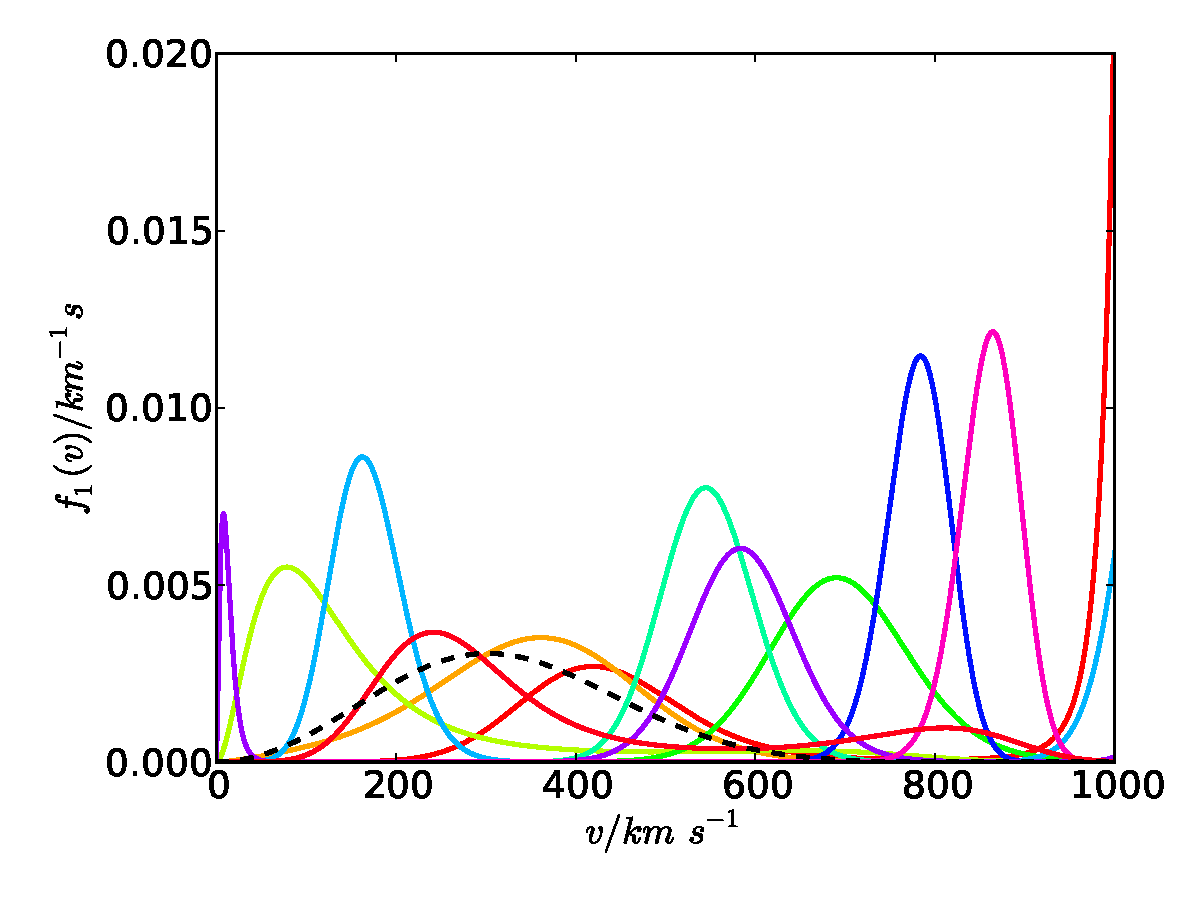
\includegraphics[width=0.75\textwidth]{Poly/Poly.pdf}
  \caption[Examples of $\ln f(v)$ polynomial distributions]{Examples of speed distributions $f_1(v)$ generated using the polynomial parametrisation for $\ln f(v)$ with $N=5$ basis functions. The SHM distribution function in the Earth frame is shown as a black dashed line for comparison.}
  \label{fig:Poly:examples}
\end{figure}


\section{Experiments and benchmark parameters}
\label{sec:Poly:experiments}

In order to generate mock data sets, we consider three idealized mock experiments, loosely based on detectors which are currently in development. The three target materials we consider here are Xenon, Argon and Germanium. As in Chapter~\ref{ch:Speed}, we describe each experiment in terms of the mass number $A$ of the target nucleus, fiducial detector mass $m_\textrm{det}$, efficiency $\epsilon$ and energy sensitivity window $\left[E_\textrm{min}, E_\textrm{max}\right]$. We consider a total exposure time for all experiments of $t_\textrm{exp} = \textrm{ 2 years}$. The experimental parameter values used in this chapter are summarized in Tab.~\ref{tab:Poly:experiments}. We note that these values may be slightly adjusted or updated compared to those used in Chapter~\ref{ch:Speed} as a result of updated experimental results and projections. We have tried to indicate the source of the values used in Tab.~\ref{tab:Poly:experiments}.

\begin{table}[t]
  \setlength{\extrarowheight}{2pt}
  \begin{center}
%\begin{sideways}
	\begin{tabular}{c|m{1.2cm}m{2.2cm}m{2cm}m{2.1cm}}
        \hline\hline
	Experiment  & Target Mass, $A$ & Detector Mass (fid.), $m_\textrm{det}$/kg & Efficiency, $\epsilon$ & Energy Range/keV\\
	\hline
	Xenon  & 131  & 1100 \cite{Aprile:2012a} & 0.7 \cite{Aprile:2012b} & 7-45 \cite{Aprile:2010} \\
	Argon  & 40  & 1000 & 0.9 \cite{Benetti:2007} & 30-100 \cite{Grandi:2005} \\
        Germanium  & 73  & 150 \cite{Bauer:2013b} & 0.6 \cite{Bauer:2013a} & 8-100 \cite{Bauer:2013a} \\
        \hline\hline
	\end{tabular}
%\end{sideways}
  \end{center}
\caption[Parameter values used for the three mock experiments used in Chapter \ref{ch:Poly}]{Summary of experimental parameters used in this work, defined in Sec.~\ref{sec:Poly:experiments}. An exposure of $t_\textrm{exp} = 2 \textrm{ years}$ is used for all 3 experiments.}
\label{tab:Poly:experiments}
\end{table}

%The exact parameter values we used in this work do not strongly impact the results we present. However, it is important to note that the total mass and exposure of the experiments will affect the total number of events observed. This in turn will affect the precision of the reconstructions. For example, we have chosen a total Argon mass of 1000 kg. This is the stated target for Argon-based experiments which are in development (e.g. Ref.~\cite{Badertscher:2013}), though at present typical fiducial masses for Argon prototypes are of the order of 100 kg \cite{Grandi:2005}. The data we have generated does not represent the `high-statistics' regime: across all three experiments the total number of events observed is roughly 200-300 with as few as 10 events in the Germanium detector for some scenarios. Using a smaller exposure (or equivalently a smaller interaction cross section) will reduce the precision of the results, but should not introduce any additional bias. We also briefly consider the impact of a \textit{larger} number of events in Sec.~\ref{sec:Poly:Recon}.


As in Chapter~\ref{ch:Speed}, we assume that SI interactions dominate and use a single value of the interaction cross section $\sigmapsi = 10^{-45} \cmsq$. However, we will consider a range of WIMP masses from 10 GeV, below which the sensitivity of current direct detection experiments decreases dramatically, up to 1000 GeV above which sensitivity to the precise WIMP mass is lost.

We consider several benchmark speed distributions in this chapter, including the SHM and the SHM with the addition of a moderate dark disk which accounts for 23\% of the total WIMP density \cite{Pillepich:2014}. For the SHM, we assume a fixed DM density of $\rho_0 = 0.3 \textrm{ GeV cm}^{-3}$. However, we treat the dark disk as an overdensity contributing an \textit{additional} WIMP population, bringing the local density up to $\rho_0 = 0.39 \textrm{ GeV cm}^{-3}$. In addition, we also use the speed distribution of Lisanti et al.~\cite{Lisanti:2010}, which has the following form in the Earth's frame:
\begin{equation}
\label{eq:Poly:lisanti}
f(\textbf{v}) = N \left[\exp\left(\frac{v_\textrm{esc}^2 - |\textbf{v} - \textbf{v}_0|^2}{k v_0^2}\right) -1\right]^k \Theta(v_\textrm{esc} - |\textbf{v} - \textbf{v}_0|)\,.
\end{equation}
We use the parameter values $k = 2$ and $v_0 = 220 \kms$ in this work. In all cases, we assume a fixed value of the escape speed $\vesc = 544 \kms$ (see Chapter~\ref{ch:DD}). We summarize in Tab.~\ref{tab:Poly:distributions} the different speed distributions considered. We also plot several of these in Fig.~\ref{fig:Poly:Ensemble_distributions} for reference.

\begin{table}[t]
  \setlength{\extrarowheight}{2pt}
  \setlength{\tabcolsep}{3pt}
  \begin{center}
	\begin{tabular}{m{3cm}|ccc}
        \hline \hline
	Speed distribution benchmark & Fraction & $v_\textrm{lag} / \kms$ & $\sigma_v / \kms$ \\
        \hline
	SHM & 1 & 220 & 156 \\
	\hline
	\multirow{2}{*}{SHM+DD} & 0.77 & 220 & 156 \\
	& 0.23 & 50 & 50 \\
	\hline
	Stream & 1 & 400 & 20 \\
	\hline
	\multirow{2}{*}{Bump} & 0.97 & 220 & 156 \\
	& 0.03 & 500 & 20 \\
	\hline
	\multirow{2}{*}{Double-peak} & 0.5 & 200 & 20 \\
	& 0.5 & 400 & 20 \\
	\hline
	Lisanti et al. & & $v_0 = 220 \kms$ & $k = 2$ \\
        \hline \hline
	\end{tabular}
        
  \end{center}
\caption[Summary of speed distribution benchmarks used in Chapter \ref{ch:Poly}]{Summary of speed distribution benchmarks used in this work. Some benchmarks are modelled as mixtures of two gaussian components, for which we give the fractional contribution of each component (labelled `Fraction'). The remaining parameters are defined in Sec.~\ref{sec:DD:astrounc}, as well as Eq.~\ref{eq:Poly:lisanti} and the accompanying text. The `bump' and `double-peak' distributions are discussed in Sec.~\ref{sec:Poly:test}. For each benchmark distribution, we fix $\vesc = 544 \kms$.}
\label{tab:Poly:distributions}
\end{table}

\begin{figure}[t]
\centering
  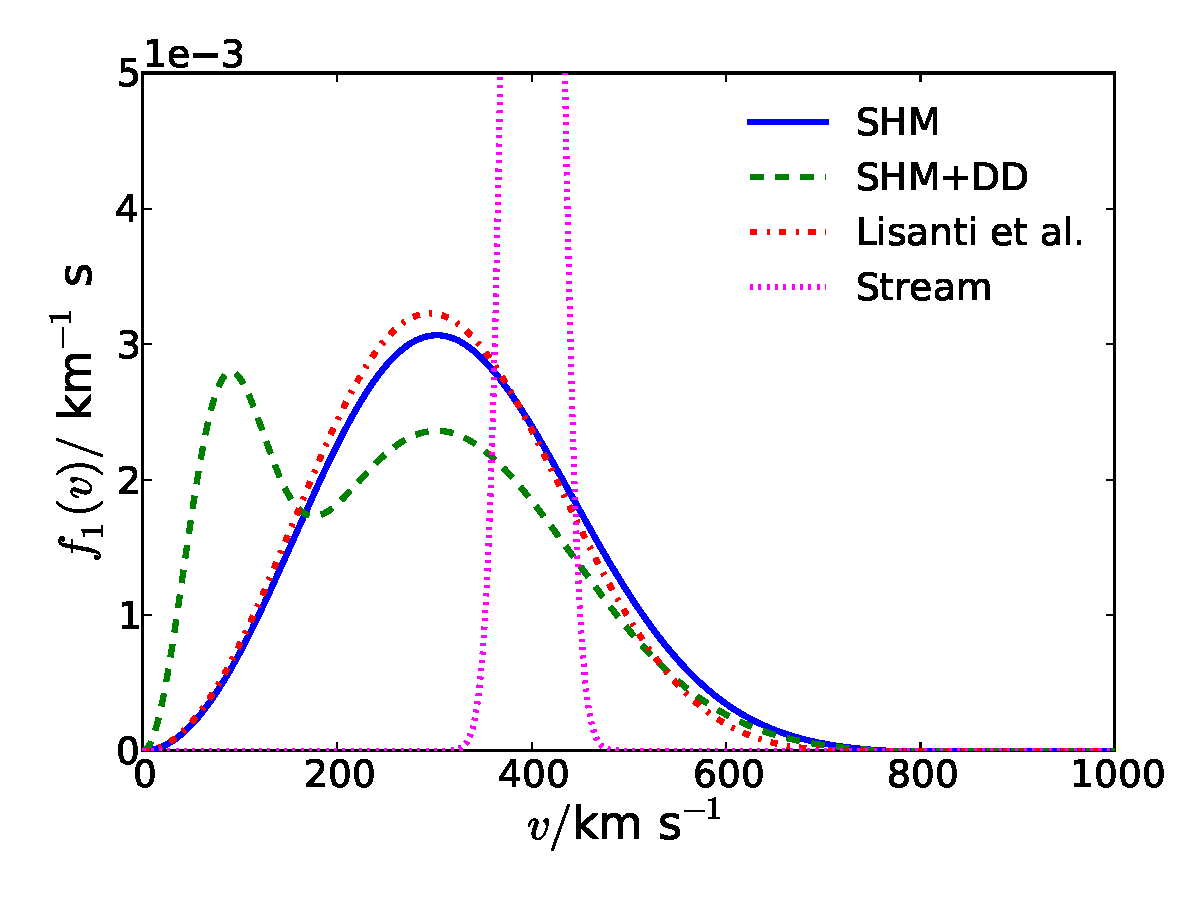
\includegraphics[width=0.75\textwidth]{Poly/SpeedDistributions-Ensemble.pdf}
  \caption[Several benchmark speed distributions used to test the polynomial $\ln f(v)$ method.]{Several of the benchmark speed distributions used in this chapter. They are defined in Eqs.~\ref{eq:gaussian} and \ref{eq:lisanti} with parameters from Tab.~\ref{tab:Poly:distributions}. These distributions are the SHM (solid blue), SHM+DD (dashed green), Lisanti et al. (dot-dashed red) and the stream (dotted magenta). Reproduced from Ref.~\cite{Kavanagh:2014}.}
  \label{fig:Poly:Ensemble_distributions}
\end{figure}


\subsection{Parameter sampling}
\label{sec:Poly:ParamRecon}
The parameter space of the polynomial $\ln f(v)$ parametrisation is much larger than for the binned method and is poorly explored using conventional MCMC methods. We therefore make parameter inferences using the publicly available \multinest nested sampling package \cite{Feroz:2007,Feroz:2008,Feroz:2014}. This allows us to map out both the likelihood $\mathcal{L}(\mathbf{\theta})$ and posterior probability distribution $\mathcal{P}(\mathbf{\theta})$ for the model parameters $\mathbf{\theta}$. We summarize in Tab.~\ref{tab:Poly:MultiNest} the \multinest sampling parameters used. We also summarize the priors used in this work in Tab.~\ref{tab:Poly:priors}. 


\begin{table}[t]
  \setlength{\extrarowheight}{2pt}
  \setlength{\tabcolsep}{3pt}
  \begin{center}
	\begin{tabular}{c|c}
        \hline\hline
        Parameter & Value \\
        \hline
	$N_\textrm{live}$ & 10000 \\
	efficiency & 0.25 \\
	tolerance & $10^{-4}$ \\
        \hline\hline
	\end{tabular}
  \end{center}
\caption[Summary of the \multinest sampling parameters used in Chapter \ref{ch:Poly}]{Summary of the \multinest sampling parameters used in this chapter.}
\label{tab:Poly:MultiNest}
\end{table}

\begin{table}[t]
  \setlength{\extrarowheight}{2pt}
  \setlength{\tabcolsep}{3pt}
  \begin{center}
	\begin{tabular}{m{1in}|cc}
        \hline\hline
	Parameter & Prior type & Prior range\\
	\hline
	$m_\chi / \textrm{ GeV}$ &  log-flat & $\left[10^{0}, 10^{3}\right]$\\
	$\sigma_p / \textrm{ cm}^2$ & log-flat & $\left[10^{-46}, 10^{-42}\right]$ \\
	$\left\{a_k\right\}$ & linear-flat & $\left[-50, 50\right]$ \\
        $R_{BG} / \textrm{dru}$ & log-flat & $\left[10^{-12}, 10^{-5}\right]$ \\
        \hline\hline
	\end{tabular}
  \end{center}
\caption[Summary of the priors on the parameters used in Chapter \ref{ch:Poly}]{Summary of the priors on the parameters used in this chapter. The background rate $R_{BG}$ is defined in Sec.~\ref{sec:Poly:mass} while the $\left\{a_k\right\}$ are the polynomial coefficients used in the parametrisation.}
\label{tab:Poly:priors}
\end{table}


In Sec.~\ref{sec:Poly:stats} and Sec.~\ref{sec:Poly:Recon}, we consider many realisations of data, including the effects of Poisson noise. We therefore use the unbinned likelihood of Eq.~\ref{eq:Speed:unbinnedL} in \multinest. As in Chapter~\ref{ch:Speed}, we make parameter inferences from the marginalised posterior distribution $\mathcal{P}_m$. We take the mode of the distribution to be the reconstructed parameter value and construct p\% \textit{minimal} credible intervals. This method performs well for small numbers of observations (compared to the number of free parameters in the fit). It is therefore a sensible choice here, where in some cases the number of events observed in an experiment is less than 10.

In Sec.~\ref{sec:Poly:test} and Sec.~\ref{sec:Poly:mass}, we consider the effects of varying the form of the parametrization and of varying the input WIMP mass. In order to eliminate the effects of Poisson noise, we use Asimov data \cite{Cowan:2013} for these sections. This means that we divide the energy window of each experiment into bins of width 1 keV. We then set the observed number of events $N_{o}^{i}$ in bin $i$ equal to the expected number of events $N_{e}^{i}$ and use the binned likelihood

\begin{equation}
\label{eq:Poly:binnedL}
\mathcal{L} = \prod_{i = 1, N_\textrm{bins}} \frac{(N_e^i)^{N_o^i}}{(N_o^i)!}e^{-N_e^i}\,,
\end{equation}
for each experiment. In these sections, we have a very large number of observations, namely the exact (non-integer) event numbers in each energy bin. We can therefore use the best fit point (i.e. the point which maximises the likelihood) as the reconstructed value. To obtain confidence intervals on some subset of the full parameter space, we use the profile likelihood $\mathcal{L}_p$, obtained by maximising $\mathcal{L}$ over the remaining nuisance parameters. We then construct confidence intervals using the asymptotic $\chi^2$ distribution of the profile likelihood \cite{Wilks:1938}.
%The profile likelihood can also lead to less noisy reconstructions than the marginalized posterior, especially when the dimensionality of the parameter space becomes high, as in Sec.~\ref{sec:Parametrization} and Sec.~\ref{sec:mass}.

%\note{Cite that new statistical paper...}

%\note{Say that we're focusing on just the SI cross section...}

\section{Results}
\label{sec:Poly:results}

Before we consider in detail the properties of the parametrisation, we show a single reconstruction of $m_\chi$ and \sigmapsi using as input a WIMP of mass 50 GeV and the SHM distribution function. We generate Asimov data for this benchmark and fit using $N=5$ basis functions and a basis of Chebyshev polynomials (see Sec.~\ref{sec:Poly:test}). If the polynomial $\ln f(v)$ parametrisation cannot produce an unbiased reconstruction of the WIMP parameters for the simple and smooth SHM benchmark, it is unlikely to be useful for more complicated distribution functions.

The results of this reconstruction are shown in Fig.~\ref{fig:Poly:2D}. There is very good agreement between the best fit point (green triangle) and the benchmark values (dashed red lines). The WIMP mass is well reconstructed, with an uncertainty of about 30\% at the $1\sigma$ level. However, we notice that there is a significant degeneracy, with the reconstruction for \sigmapsi extending up to large values. This problem was discussed briefly in Chapter~\ref{ch:Speed}. We have no information about the shape of $f(v)$ below the energy thresholds of the experiments. This means that distributions which have a large WIMP population at low speeds can be made to fit the data as well as those which do not, as long as the value of the cross section is adjusted to compensate. While we can reconstruct $m_\chi$ using this method, we can only place a lower limit on \sigmapsi unless we make further assumptions about the low speed WIMP population. We will now explore in more detail the properties of this new parametrisation method.

\begin{figure}[t]
\centering
  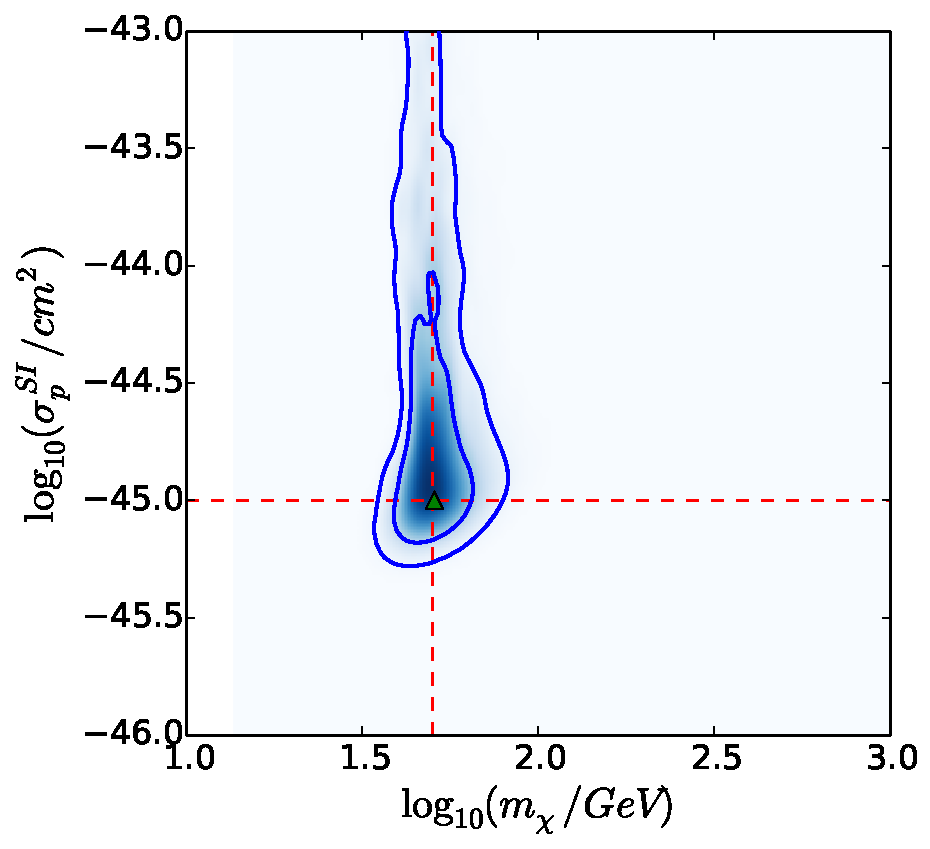
\includegraphics[width=0.75\textwidth]{Poly/SHM_50_ASIMOV.pdf}
  \caption[Reconstruction of the WIMP mass and cross section using the polynomial $\ln f(v)$ parametrisation]{Reconstruction of the WIMP mass and cross section using the polynomial $\ln f(v)$ parametrisation with 5 basis functions. Asimov data was generated for a WIMP with $m_\chi = 50 \textrm{ GeV}$ and $\sigmapsi = 10^{-45} \cmsq$ (shown as dashed red horizontal and vertical lines) and the SHM speed distribution. The shaded blue shows the value of the profile likelihood (with darker values corresponding to higher likelihood), along with the 68\% and 95\% confidence contours. The best fit point is shown as a green triangle.}
  \label{fig:Poly:2D}
\end{figure}


%We compare the performance of the polynomial $\ln f(v)$ presented here with the binned distribution functions of the previous chapter. We use a 50 GeV WIMP with a stream distribution function \note{defined where?} and, using a single realisation of data, attempt to reconstruct the WIMP mass using each method. The results are shown in Table~\ref{tab:Poly:ReconstructedMass}. The polynomial $\ln f(v)$ method shows a clear improvement over the other two methods. Not only is the parametrised distribution smooth, removing the need for any fixed lengthscales, but it is also better able to capture the rapidly varying form of the stream distribution function. \note{Redo this, I don't think I want to use the stream...}

\begin{comment}
\begin{table}[t]
  \setlength{\extrarowheight}{5pt}
  \begin{center}
	\begin{tabular}{lc}
         \hline\hline
	 Parametrisation & Reconstructed mass (GeV) \\
	 \hline
	 Polynomial $\ln f(v)$ & \(44.7^{+6.9}_{-3.6}\) \\
	 Binned $f(v)$ & \(29.3^{+0.4}_{-1.0}\) \\
	 Binned $\tilde{f}(p)$ & \(38.2^{+1.6}_{-2.3}\)\\
         \hline\hline
	\end{tabular}
  \end{center}
  \caption[Reconstructed mass for a 50 GeV WIMP using the speed binning, momentum binning and polynomial $\ln f(v)$ parametrisations]{Reconstructed mass using the parametrization presented in this chapter, as well as the the speed binning and momentum binning methods of Chapter~\ref{ch:Speed} for comparison. The benchmark used is a stream distribution function described in \note{Somewhere!} and a 50 GeV WIMP. In all cases, 5 speed distribution parameters (either bins or basis coefficients) are used.}
\label{tab:Poly:ReconstructedMass}
\end{table}
\end{comment}

\subsection{Testing the parametrisation}
\label{sec:Poly:test}

We now consider the two questions: \begin{inparaenum}[(i)] \item how many basis functions are required and \item which polynomial basis should be used? \end{inparaenum} In order to answer these questions, we use the two benchmark distribution functions illustrated in Fig.~\ref{fig:Poly:VaryingN_distributions}. We have chosen these benchmarks not because they are necessarily realistic distribution functions but because they should be difficult to fit using standard techniques and fitting functions (e.g.~\cite{Lisanti:2010}). The first distribution (referred to as `bump') is a SHM distribution with the addition of a small bump, which contributes just 3\% of the total WIMP population and could correspond to a small sub-halo or stream \cite{Vogelsberger:2009}. This should be difficult to fit because it represents only a very small deviation from the standard scenario. The second distribution (referred to as `double-peak') has a sharp and rapidly varying structure, which we anticipate should be difficult to capture using a small number of basis functions.

\begin{figure}[t]
\centering
  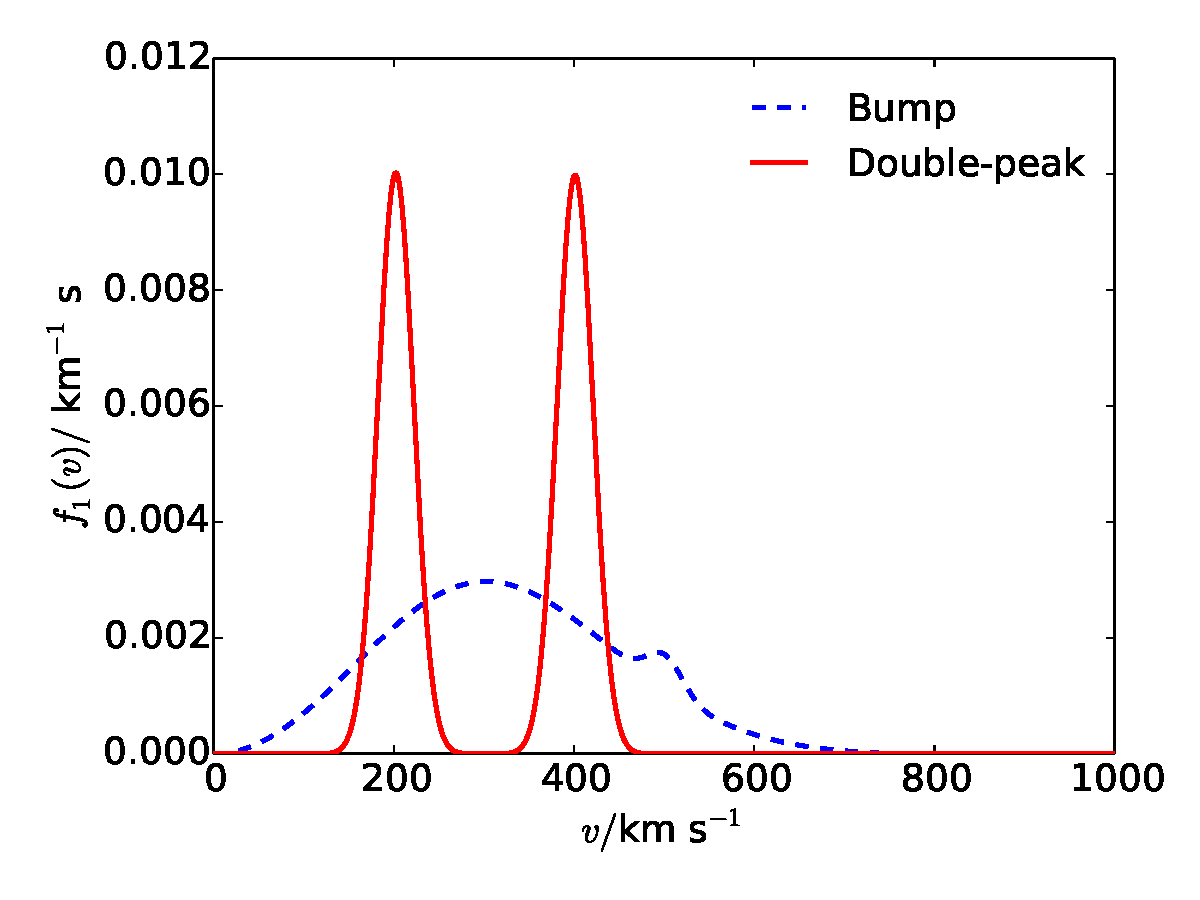
\includegraphics[width=0.75\textwidth]{Poly/SpeedDistributions-VaryingN.pdf}
  \caption{Benchmark speed distributions used in Sec.~\ref{sec:Poly:test} to test the performance of the parametrization as a function of the number and type of basis functions. Reproduced from Ref.~\cite{Kavanagh:2014}.}
  \label{fig:Poly:VaryingN_distributions}
\end{figure}

\subsubsection{Varying the number of basis functions}

We first investigate how the reconstructed WIMP mass $m_\textrm{rec}$ and uncertainty varies with the number of basis functions $N$. For now, we fix our choice of basis to shifted Legendre polynomials\footnote{We use the shifted argument $2v/v_\textrm{max} - 1$ in order to enforce the orthogonality of the polynomials over the range $v \in [0, v_\textrm{max}]$.}:
\begin{equation}
P_k(v) = L_k\left(2\frac{v}{v_\textrm{max}} - 1\right)\,,
\end{equation}
where $L_k$ is the Legendre polynomial of order $k$.
 
The lower panel of Fig.~\ref{fig:Poly:BUMP_LEG} shows the best fit mass and 68\% confidence intervals as a function of $N$, using as input a WIMP of mass 50 GeV and the `bump' distribution function. The reconstructed mass very rapidly settles close to the true value, using as few as three basis functions. This is because adding the bump near $v \sim 500 \kms$ still leaves the mean inverse speed relatively smooth, so a large number of basis functions is not required. The correct mass is reconstructed and we emphasize in the lower panel of Fig.~\ref{fig:Poly:BUMP_LEG} that the reconstruction is stable with the addition of more basis functions.

We should also consider how the quality of the fit changes as a function of $N$. We would expect that adding fit parameters should always lead to a better fit. Eventually, the fit should be good enough that adding additional basis functions will no longer improve it significantly. We can then be confident that our reconstruction is accurate and not an artifact of using too few basis functions. In order to investigate this, we utilise the Bayesian Information Criterion (BIC) \cite{Schwarz:1978}, which is given by:

\begin{equation}
BIC = 2N_p\textrm{ln}(N_m) - \textrm{ln}(\mathcal{L}_\textrm{max}) \, ,
\end{equation}
where $N_p$ is the number of free parameters, $N_m$ is the number of measurements or observations and $\mathcal{L}_\textrm{max}$ is the maximum likelihood value obtained in the reconstruction. For the case of binned data, $N_m$ corresponds simply to the total number of energy bins across all experiments. This criterion penalises the inclusion of additional free parameters and in comparing several models, we should prefer the one which minimises the BIC.

\begin{figure}[t!]
\centering
  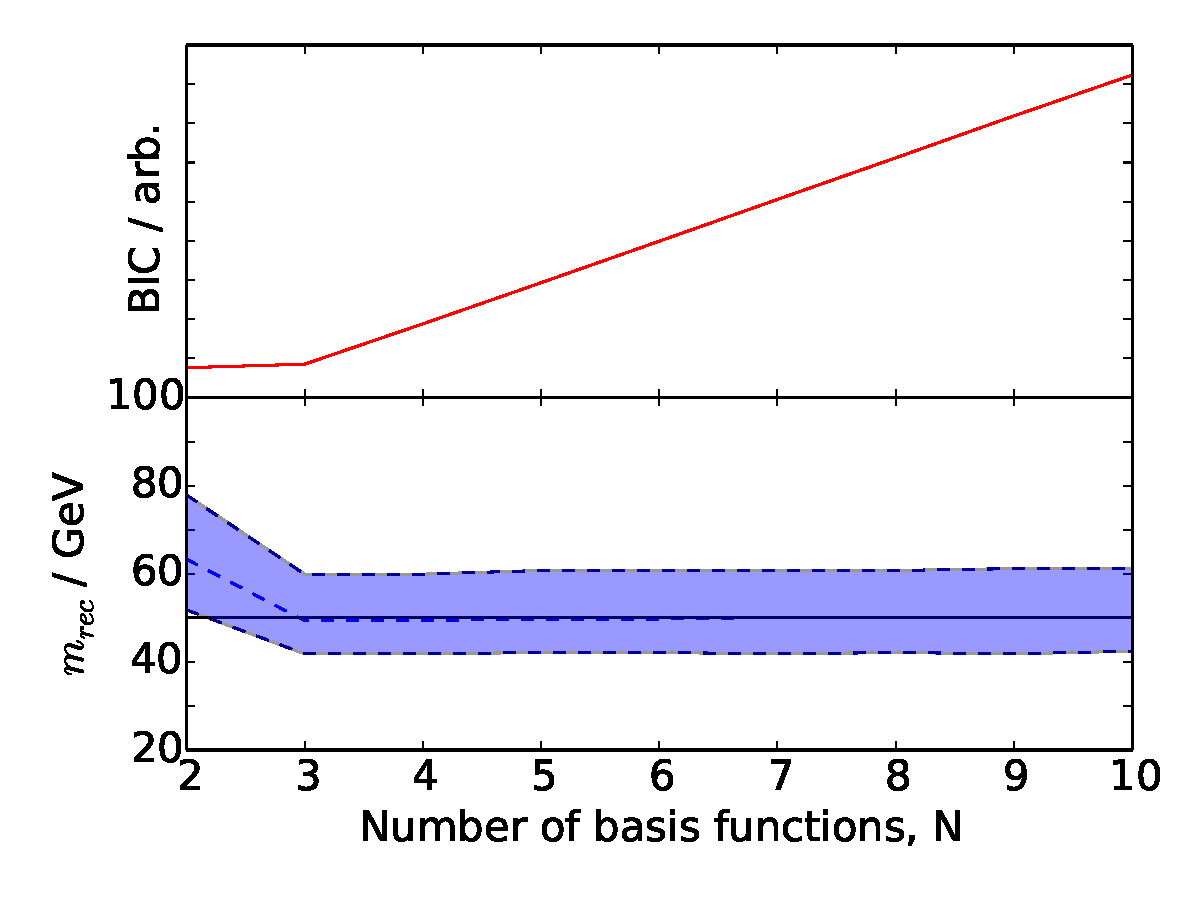
\includegraphics[width=0.75\textwidth]{Poly/VaryingN_BUMP_LEG.pdf}
  \caption[Bayesian information criterion and reconstructed WIMP mass as a function of the number of basis functions for a 50 GeV WIMP with `bump' distribution function]{Bayesian information criterion (BIC) as a function of the number of basis functions for an underlying `bump' distribution function, 50 GeV WIMP and using Legendre polynomial basis functions (upper panel). Also shown (lower panel) are the reconstructed WIMP mass (dashed blue line), 68\% confidence interval (shaded blue region) and underlying WIMP mass (solid horizontal black line). Reproduced from Ref.~\cite{Kavanagh:2014}.}
  \label{fig:Poly:BUMP_LEG}
\end{figure}

The upper panel of Fig.~\ref{fig:Poly:BUMP_LEG} shows the BIC (in arbitrary units) as a function of the number of basis functions for the `bump' distribution function. The BIC is comparable for the cases of $N=2$ and $N=3$, indicating that the quality of the fit is improved slightly by the addition of another basis function. However, adding further basis functions does not have a significant impact on the maximum likelihood, leading to an increase in the BIC. This coincides with the stabilization of the reconstructed mass around the true value and we conclude that only two or three basis functions are required to provide a good fit to the data.

\begin{figure}[t!]
\centering
  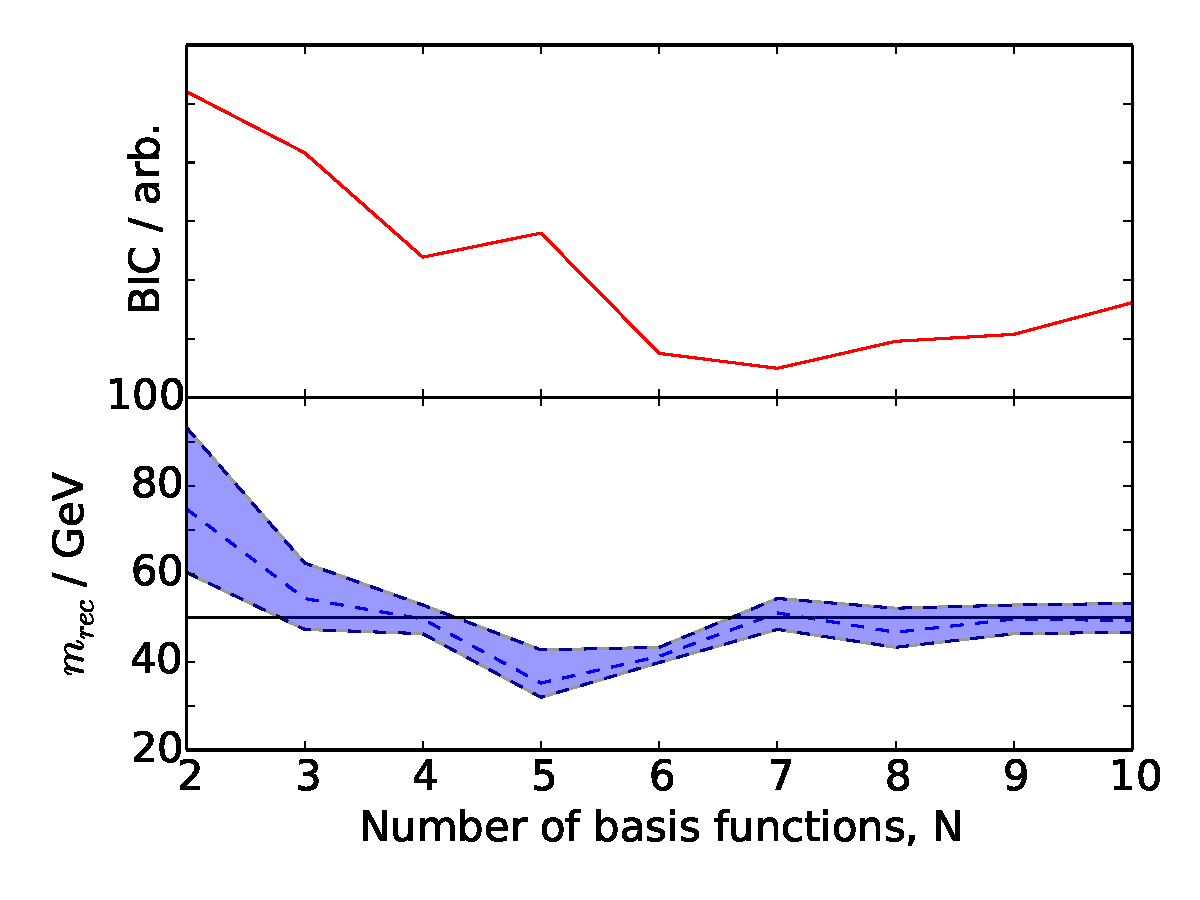
\includegraphics[width=0.75\textwidth]{Poly/VaryingN_DP_LEG.pdf}
  \caption{As Fig.~\ref{fig:Poly:BUMP_LEG} but for an underlying `double-peak' distribution function. Reproduced from Ref.~\cite{Kavanagh:2014}.}
  \label{fig:Poly:DP_LEG}
\end{figure}

Figure \ref{fig:Poly:DP_LEG} shows the corresponding results for the `double-peak' distribution function. Here, we note that the bias induced by using too small a number of basis functions is larger than for the case of the `bump' distribution, due to the more complicated structure in this case. The BIC is minimized for $N=7$, indicating that additional basis functions do not significantly improve the quality of the fit to data. This suggests that the shape of the speed distribution can be well fit by $N\geq7$ basis functions. As shown in the lower panel of Fig.~\ref{fig:Poly:DP_LEG}, the reconstruction of the WIMP mass is stable around the true mass for these values of $N$.

We propose that such a procedure should be used in the case of real data should a dark matter signal be observed at multiple detectors. We have shown that by analyzing the reconstructed mass as a function of $N$ we can recover the true mass and that by using the BIC we can be confident that we have obtained an adequate fit to data.

\subsubsection{Choice of basis functions}

We now consider the second question posed at the start of Sec.~\ref{sec:Poly:test}: which polynomial basis should be used? As previously mentioned, we test two different polynomial bases: Legendre and Chebyshev polynomials. We have checked that the reconstruction results using Chebyshev polynomials are largely indistinguishable from the case of Legendre polynomials for both the `bump' and `double-peak' distributions and as a function of $N$. This leads us to conclude that the accuracy of the reconstruction is independent of the specific choice of basis. However, the reconstruction was much faster in the case of the Chebyshev basis. This is illustrated in Fig.~\ref{fig:Poly:times}, which shows the time taken for reconstruction of the `bump' benchmark as a function of $N$. The time taken grows much more slowly for the Chebyshev basis (roughly as $N^2$) than for the Legendre basis (roughly as $N^3$). This is consistent with the common use of the Chebyshev basis in polynomial approximation problems \cite{Mason:2002}. We have also checked that this difference is not an artifact of how we calculate the basis functions. These results indicate that this choice of basis provides both reliable and efficient reconstruction for the WIMP mass and we therefore use the Chebyshev basis in the remainder of this work.

\begin{figure}[ht!]
\centering
  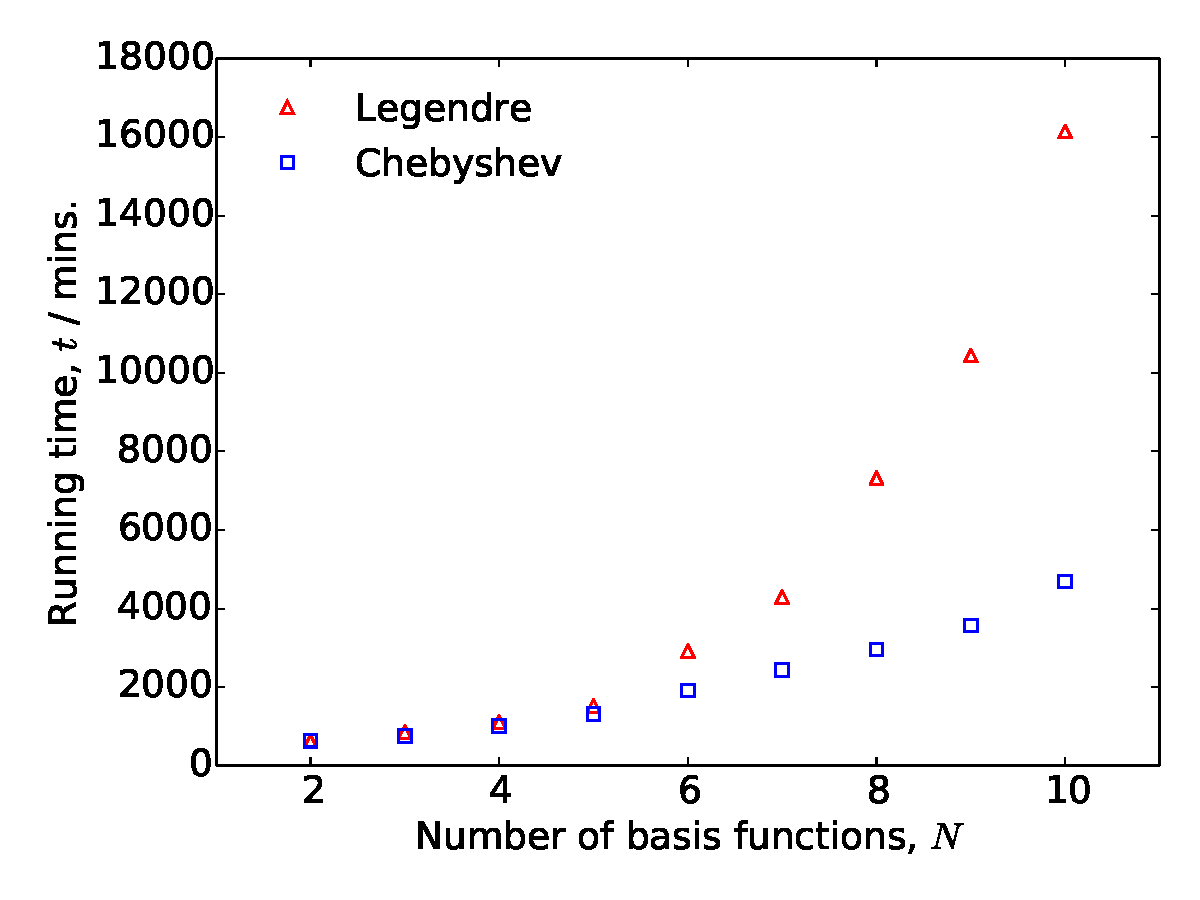
\includegraphics[width=0.75\textwidth]{Poly/RunTimes.pdf}
  \caption[Time taken for the reconstruction of the `bump' benchmark as a function of number of basis functions for both the Chebyshev and Legendre bases.]{Time taken (using 4 processors in parallel) for the reconstruction of the `bump' benchmark, as a function of number of basis functions. The time taken using the Chebyshev basis (blue squares) grows more slowly with $N$ than for the Legendre basis (red triangles). Reproduced from Ref.~\cite{Kavanagh:2014}.}
  \label{fig:Poly:times}
\end{figure}

\section{Varying $m_\chi$}
\label{sec:Poly:mass}

We now consider the performance of the parametrisation over a wide range of WIMP masses. We generate Asimov data for WIMP masses of 10, 20, 30, 40, 50, 75, 100, 200 and 500 GeV and reconstruct the best fit WIMP mass $m_\textrm{rec}$ and 68\% and 95\% confidence intervals from the profile likelihood. We use the SHM as a benchmark distribution function and use a fixed number of $N=5$ basis functions. The results are shown in Fig.~\ref{fig:Poly:VaryingM}, along with the line $m_\textrm{rec} = m_\chi$ for reference.

For large values of $m_\chi$, the shape of the event spectrum becomes independent of $m_\chi$ \cite{Green:2008}, which results in a widening of the confidence intervals as the WIMP mass increases. For low mass WIMPs, fewer events are observed in each bin, again resulting in wider confidence intervals. It should be noted that for this analysis we have used Asimov data, in which the exact (non-integer) number of events is recorded in each bin. For low mass WIMPs, this means that the spectrum (and therefore the correct WIMP mass) is still well reconstructed using Asimov data, in spite of the small number of events. The tightest constraints are obtained when the input WIMP mass is close to the masses of several of the detector nuclei (in the range 30-80 GeV). There also appears to be no bias in the WIMP mass: the reconstruction matches the true mass across all values considered.

\begin{figure}[t]
\centering
  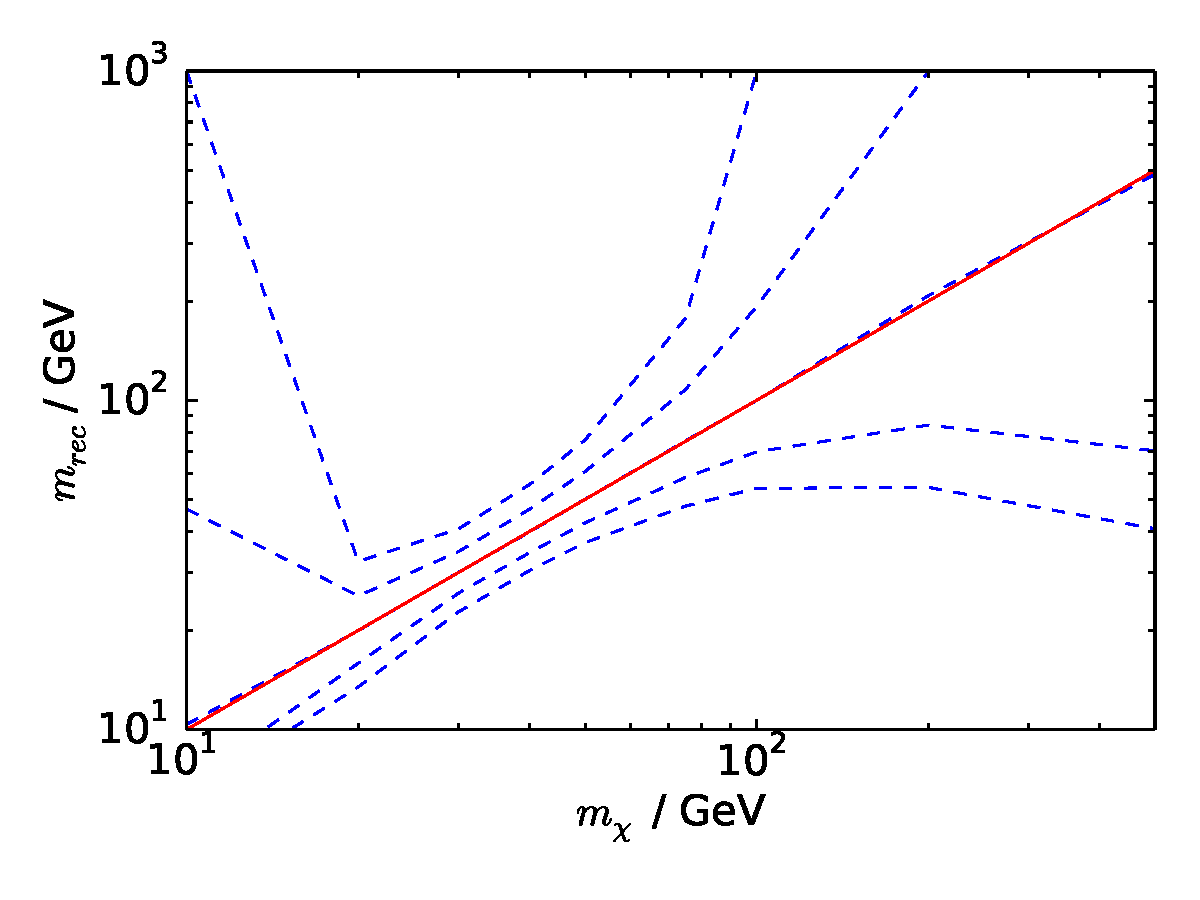
\includegraphics[width=0.75\textwidth]{Poly/VaryingM.pdf}
  \caption[Reconstructed WIMP mass as a function of input WIMP mass for ideal experiments]{Reconstructed WIMP mass $m_\textrm{rec}$ (central dashed blue line) as a function of input WIMP mass $m_\chi$ as well as 68\% and 95\% intervals (inner and outer blue dashed lines respectively). The line $m_\textrm{rec} = m_\chi$ (solid red line) is also plotted for reference. Reproduced from Ref.~\cite{Kavanagh:2014}.}
  \label{fig:Poly:VaryingM}
\end{figure}


%%%PUT THIS IN THE DISCUSSION
%As described in Chapter~\ref{ch:Speed}, for low mass WIMPs the momentum distribution may be very narrow, owing to their lower momenta. However, if we wish to parametrise the full momentum range to which the experiments are sensitive, this would be much wider. \note{Better explanation...?} The momentum parametrization method therefore performs poorly for low mass WIMPs. The parametrization presented in this chapter does not suffer from similar problems.

So far, we have only considered idealized direct detection experiments. We now apply the method to more realistic mock detectors, taking into account the effects of finite energy resolution, as well as unrejected background events. We assume here that each experiment has a gaussian energy resolution with fixed width $\sigma_E = 1 \textrm{ keV}$ (see Sec.~\ref{sec:DD:finalrate} for details). We also assume a constant flat background rate for each experiment $R_\textrm{BG} = 10^{-6}$ events/kg/keV/day (which has been suggested as a possible background rate for Xenon1T \cite{Aprile:2010} and WArP-100L \cite{Grandi:2005}) when generating mock data sets. However, we allow the flat background rate in each experiment to vary as free parameters during the fit.

We have chosen relatively generic resolution and background parameters in this work, because the precise details of energy resolution and background shape and rate will depend on the specific experiment under consideration. Instead, we hope to show that the inclusion of more realistic experimental setups does not introduce an additional bias or otherwise spoil the good properties of the method presented here.

Figure \ref{fig:Poly:VaryingM_real} shows the reconstructed mass as a function of input mass in this more realistic scenario. The 68\% and 95\% confidence intervals are now wider and the reconstructed mass does not appear to be as accurate. For input masses above $\sim$100 GeV, the uncertainties become very wide, with only a lower limit of $m_\textrm{rec} > 20 \textrm{ GeV}$ being placed on the WIMP mass.  Due to the poorer energy resolution the shape of the energy spectrum is less well-determined. In addition, a flat background contribution can mimic a higher mass WIMP, as it leads to a flatter spectrum. This leads to a strong degeneracy, as a wide range of mass values can provide a good fit to the data. For high input masses, the profile likelihood is approximately constant above $m_\textrm{rec} \sim 20 \textrm{ GeV}$, indicating that there is no sensitivity to the underlying WIMP mass.

In spite of this, the true mass values still lie within the 68\% and 95\% confidence intervals. In addition, the poor values for the reconstructed mass for heavy WIMPs are a side effect of the loss of sensitivity. Because the profile likelihood is approximately flat, the maximum likelihood point is equally likely to be anywhere within the 68\% interval. These effects would be present even if we had considered a fixed form for the speed distribution. However, when we allow for a range of possible speed distributions, the effects become more pronounced. These results show that for more realistic experimental scenarios, the method presented in this paper remains reliable over a range of masses, though its precision may be significantly reduced.

\begin{figure}[t]
\centering
  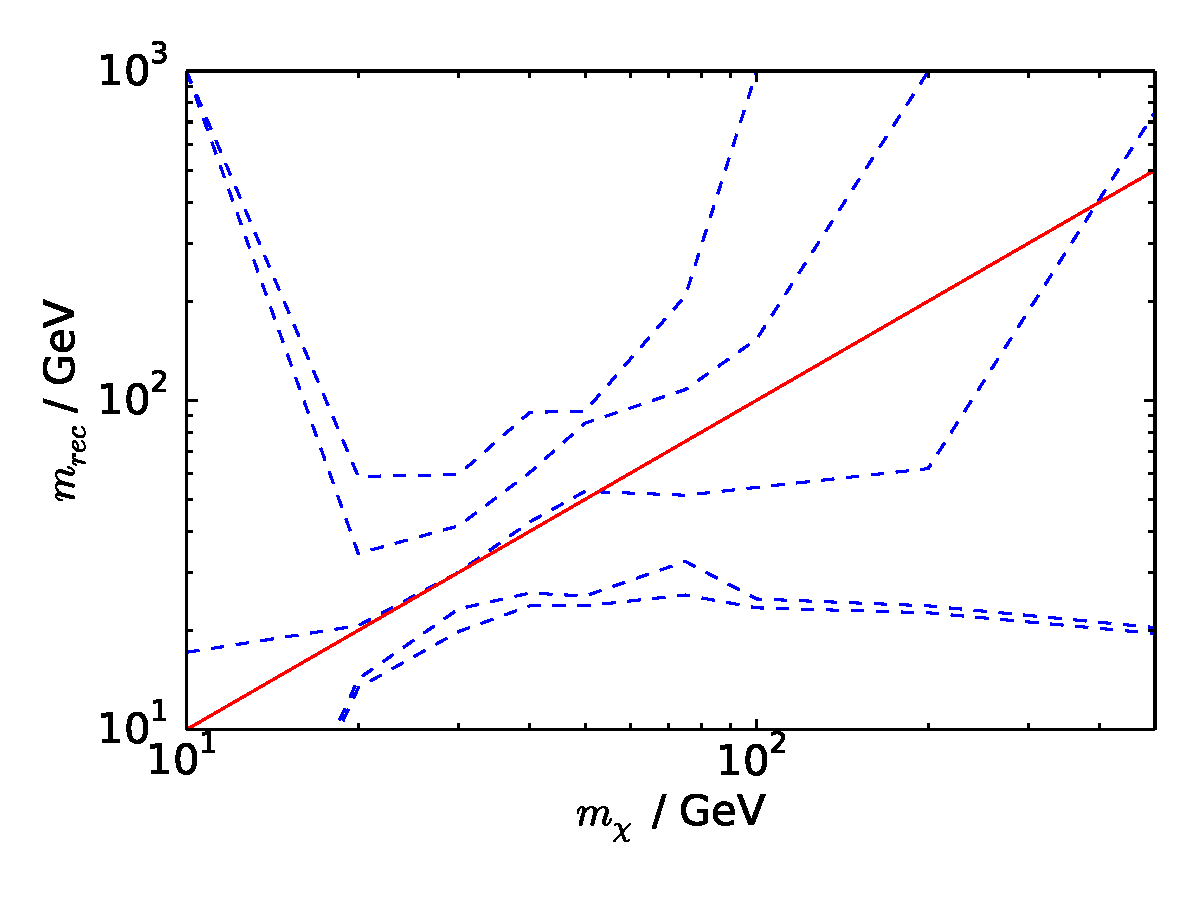
\includegraphics[width=0.75\textwidth]{Poly/VaryingM_real.pdf}
  \caption[Reconstructed WIMP mass as a function of input WIMP mass for experiments including the effects of finite backgrounds and energy resolution]{As fig.~\ref{fig:Poly:VaryingM} but including the effects of finite energy resolution and non-zero backgrounds, as described in the text. Reproduced from Ref.~\cite{Kavanagh:2014}.}
  \label{fig:Poly:VaryingM_real}
\end{figure}

\section{Statistical properties}
\label{sec:Poly:stats}

%\todo{Include the coverage maps...}

We now consider the impact of statistical fluctuations on the reconstruction of the WIMP mass. In reality, the number of events observed $N_o$ at a given experiment will be Poisson distributed about the expected value $N_e$, while the observed distribution of recoil energies will not exactly match that expected from the calculated event rate. The fundamental statistical limitations of future direct detection experiments have been studied in detail in Ref.~\cite{Strege:2012}. As in Chapter~\ref{ch:Speed}, we generate 250 realisations of data from the mock experiments described in Tab.~\ref{tab:Poly:experiments}.

For each realisation, we then use the polynomial $\ln f(v)$ parametrisation (using $N = 5$ basis functions) to reconstruct the WIMP mass and 68\% and 95\% credible intervals. Figure~\ref{fig:Poly:Realisations} shows the distribution of reconstructed masses for an input mass of 50 GeV for three benchmark speed distributions: SHM, SHM+DD and Lisanti et al.\, as described in Sec.~\ref{sec:Poly:experiments}. In all three cases, the reconstructions are peaked close to the true value, regardless of the underlying distribution. 

%For the SHM+DD distribution, the spread of reconstructions is slightly wider (with more reconstructions extending up to higher masses). This is because the 

%This is due to the smaller number of events for this benchmark, making the data sets more susceptible to Poisson fluctuations.

In order to assess the accuracy of the reconstructed value of the mass $m_\textrm{rec}$, we also calculate the bias $b$ for each realisation:

\begin{equation}
\label{eq:Poly:bias}
b = \textrm{ln}(m_\textrm{rec} / \textrm{GeV}) - \textrm{ln}(m_\textrm{true} / \textrm{GeV})\,.
\end{equation}
We compare the logarithms of the mass values because we have used logarithmically-flat priors on the WIMP mass. In Tab.~\ref{tab:Poly:bias} we show the average bias across all 250 realisations for each of the three benchmark distributions. In all three cases, the average bias is consistent with zero. Even in the SHM+DD case, which shows larger fluctuations away from the true value, there is no statistical bias.

%%%%%%%%%%%%%%%%%%%%%%%%%%%%%%%%%%%%%%%%%%%%%%%%%%%%%%%%%%%%%%%%%%%%%%%%%%%%%%%%%%%%%%%%%%%%\note{Need to specify which parametrisation is being used in the captions...}

\begin{figure}
\centering
  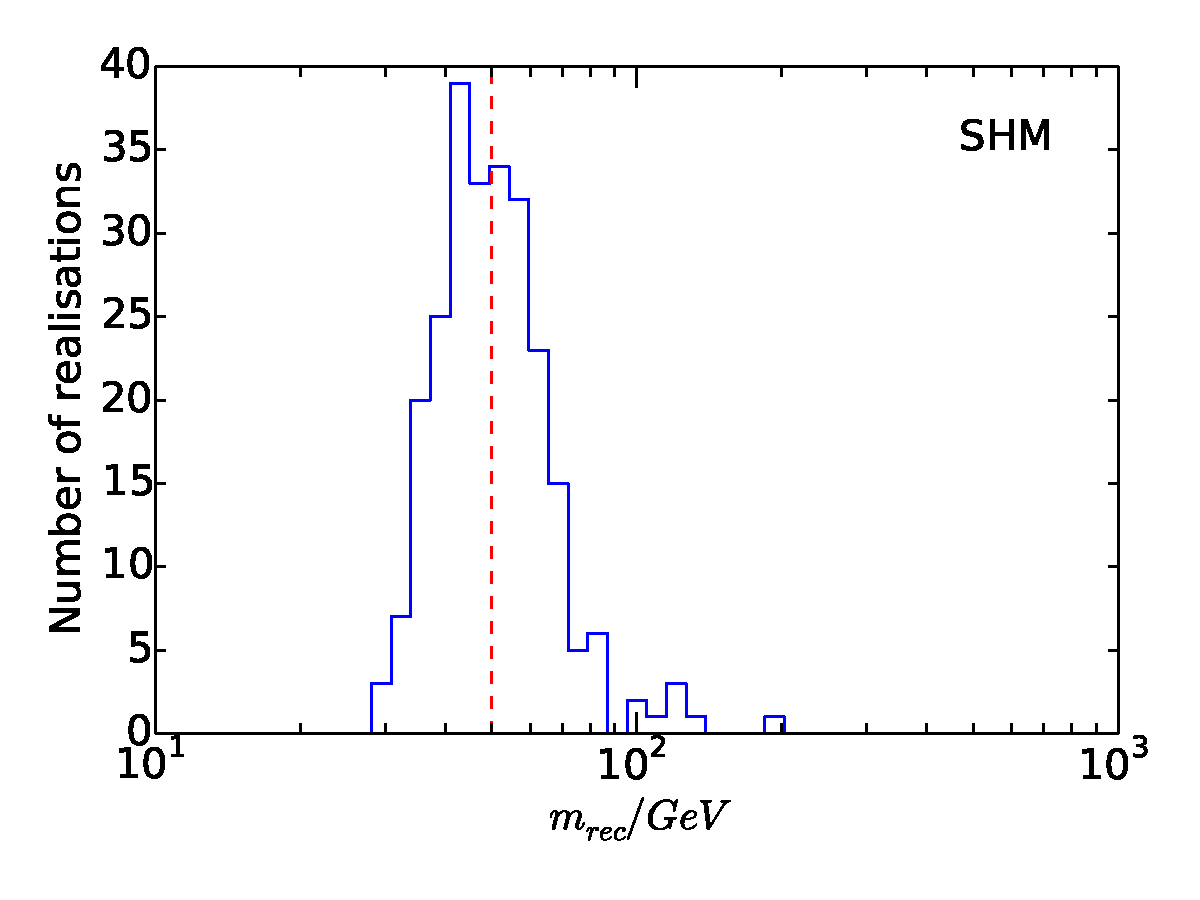
\includegraphics[trim=0cm 1cm 0cm 0.5cm,clip=true,width=0.75\textwidth]{Poly/SHM_ensemble.pdf}
  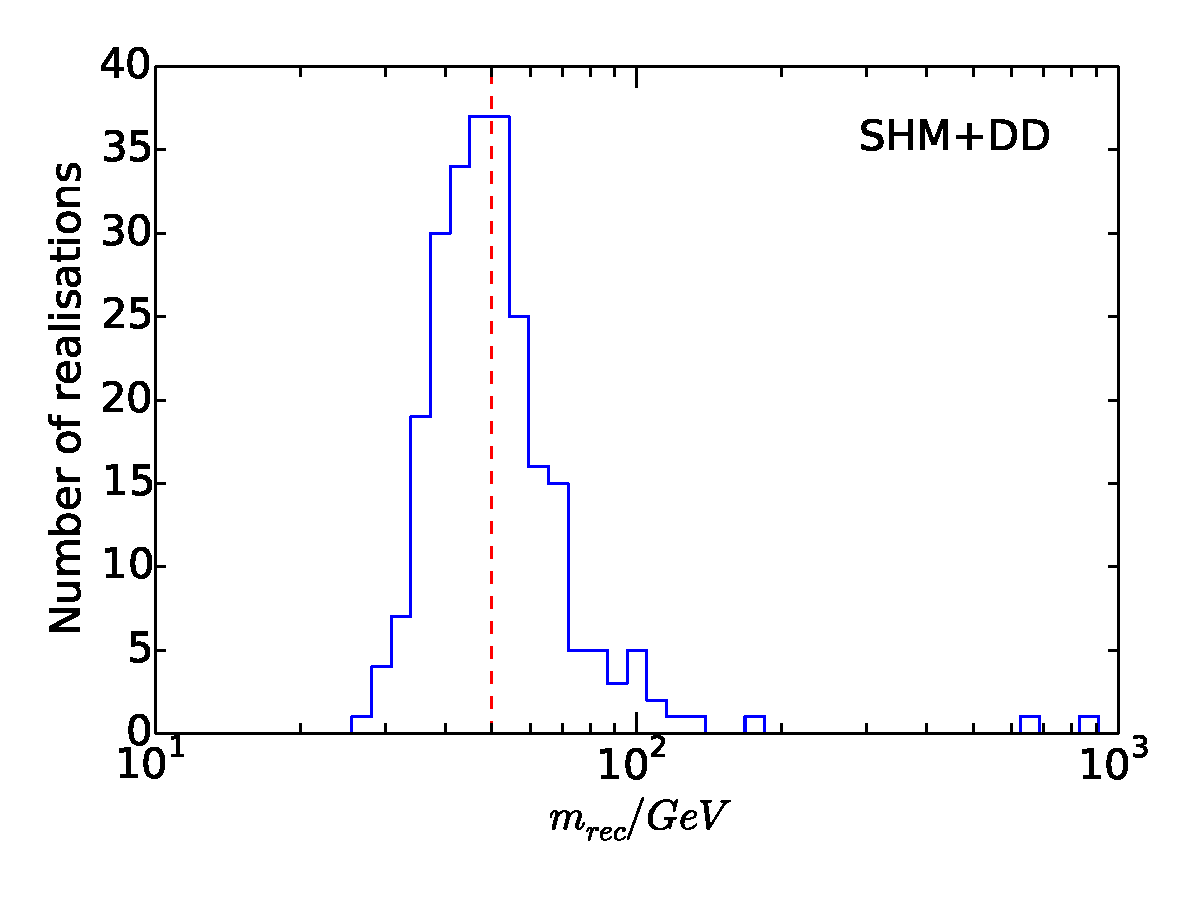
\includegraphics[trim=0cm 1cm 0cm 0.5cm,clip=true,width=0.75\textwidth]{Poly/DD_ensemble.pdf}
  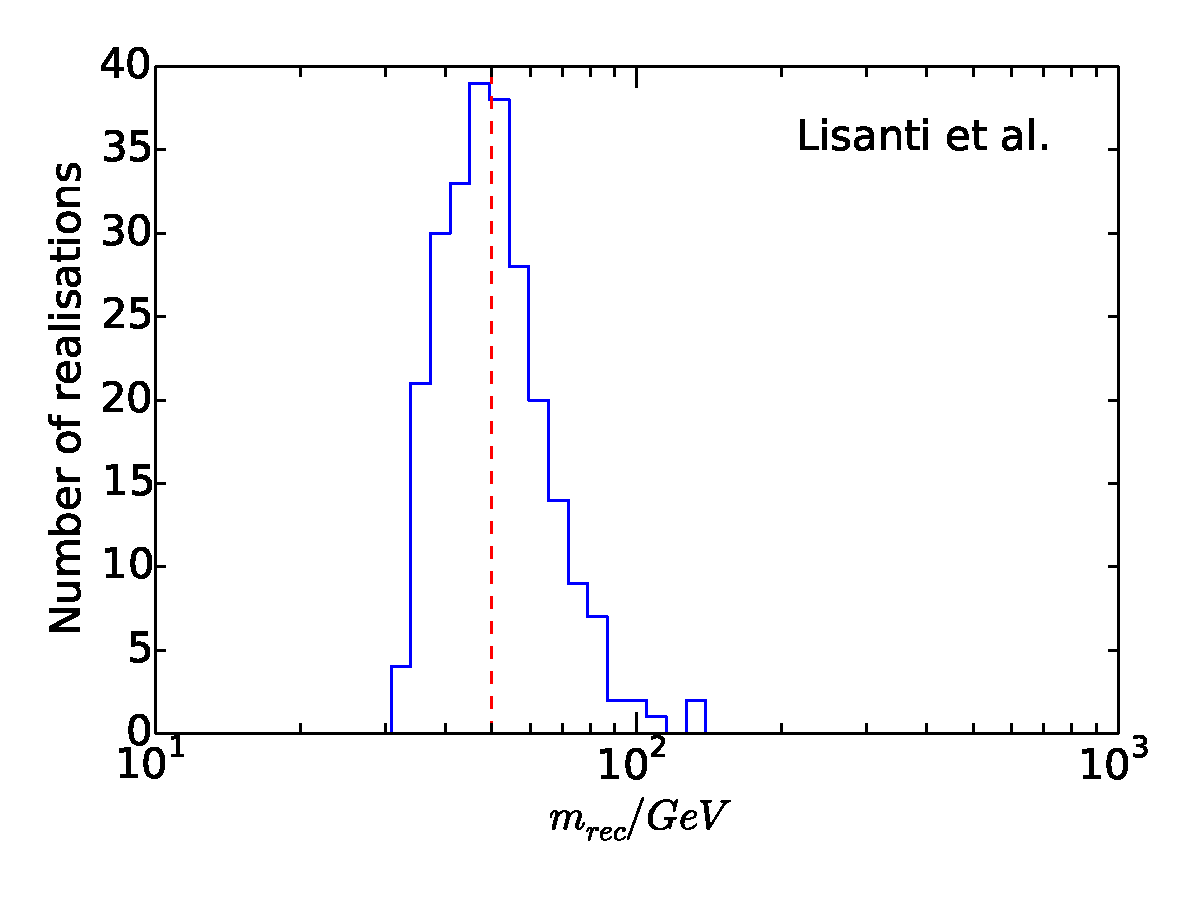
\includegraphics[trim=0cm 1cm 0cm 0.5cm,clip=true,width=0.75\textwidth]{Poly/LIS_ensemble.pdf}
  \caption[Distribution of the reconstructed mass using a 50 GeV WIMP and SHM, SHM+DD and Lisanti et al. distribution functions]{Distribution of the reconstructed mass $m_\textrm{rec}$ for 250 mock data sets generated using several benchmark speed distributions, defined in Sec.~\ref{sec:Poly:benchmarks}. These are the SHM (top), SHM+DD (middle) and Lisanti et al.\ (bottom) distributions. The input WIMP mass of $m_\chi = 50 \textrm{ GeV}$ is shown as a vertical dashed red line. Reproduced from Ref.~\cite{Kavanagh:2014}.} 
  \label{fig:Poly:Realisations}
\end{figure}

\begin{table}[t]
  \setlength{\extrarowheight}{3pt}
  \setlength{\tabcolsep}{3pt}
  \begin{center}
	\begin{tabular}{c|c}
        \hline\hline
	Benchmark distribution & Mean bias $\langle b \rangle$ \\
	\hline
	SHM & 0.002 $\pm$ 0.008 \\
	SHM+DD & 0.005 $\pm$ 0.007 \\
	Lisanti et al. & 0.01 $\pm$ 0.01 \\
        \hline\hline
	\end{tabular}
  \end{center}
\caption[Mean bias in the reconstructed log WIMP mass using the \PLF method]{Mean bias $\langle b \rangle$ in the reconstructed log WIMP mass (Eq.~\ref{eq:Poly:bias}). This was calculated over 250 realisations using three different benchmark speed distributions.}
\label{tab:Poly:bias}
\end{table}

We also test the \textit{coverage} of the credible intervals which have been constructed. Table \ref{tab:Poly:coverage} shows the coverage values for the $68\%$ and $95\%$ intervals obtained in this section. In each case, there is very close to exact coverage. We have also checked that these intervals only provide exact coverage for the true WIMP mass of 50 GeV. Other values of $m_\textrm{rec}$ are contained within the intervals less frequently than the true value, again indicating that this parametrization allows for unbiased and statistically robust reconstructions of the WIMP mass.

\begin{table}[t]
  \setlength{\extrarowheight}{3pt}
  \setlength{\tabcolsep}{3pt}
  \begin{center}
	\begin{tabular}{m{1in}|cc}
        \hline\hline
	Benchmark speed distribution & 68\% coverage & 95\% coverage\\
	\hline
	SHM &  71 $\pm$ 3 \% & 94 $\pm$ 3 \%  \\
	SHM+DD & 68 $\pm$ 3 \% & 91 $\pm$ 4 \%  \\
	Lisanti et al. & 70 $\pm$ 3 \% & 95 $\pm$ 3 \%  \\
        \hline \hline
	\end{tabular}
  \end{center}
\caption[Credible interval coverage results for the \PLF method]{Coverage of 68\% and 95\% credible intervals calculated from 250 data realisations each for three benchmark speed distributions. The concept of coverage is described in the text of Sec.~\ref{sec:Poly:stats}.}
\label{tab:Poly:coverage}
\end{table}

\section{Reconstructing $f_1(v)$}
\label{sec:Poly:Recon}

Using the method described in this chapter, we can obtain the posterior probability distribution for the coefficients $\left\{ a_1, ..., a_{N-1}\right\}$ given the data, which we refer to as $P(\textbf{a})$. We would like to be able to present this information in terms of the distribution function $f_1(v)$ in order to compare with some known distribution or look for particular features in the distribution. However, due to the fact that the distribution function is normalized, the values of $f_1$ at different speeds will be strongly correlated. We illustrate here how robust comparisons with benchmark distributions can be made.

As a first step, we can attempt to sample from $P(\textbf{a})$, in order to obtain $P(f_1(v))$. This is the probability distribution for the value of $f_1$ at a particular speed $v$, marginalizing over the values of $f_1$ at all other speeds. We can repeat for a range of speeds to obtain 68\% and 95\% credible intervals for the whole of $f_1(v)$. The result of this procedure is presented in Fig.~\ref{fig:Poly:f}, for a randomly selected realisation from the SHM ensemble of Sec.~\ref{sec:Poly:stats}. The underlying SHM distribution is shown as a solid line, while the 68\% and 95\% marginalized intervals are shown as dark and light shaded regions respectively. In this naive approach, we see that there is little shape information which can be recovered from the reconstruction, with only upper limits being placed on the speed distribution.

\begin{figure}[t]
\centering
  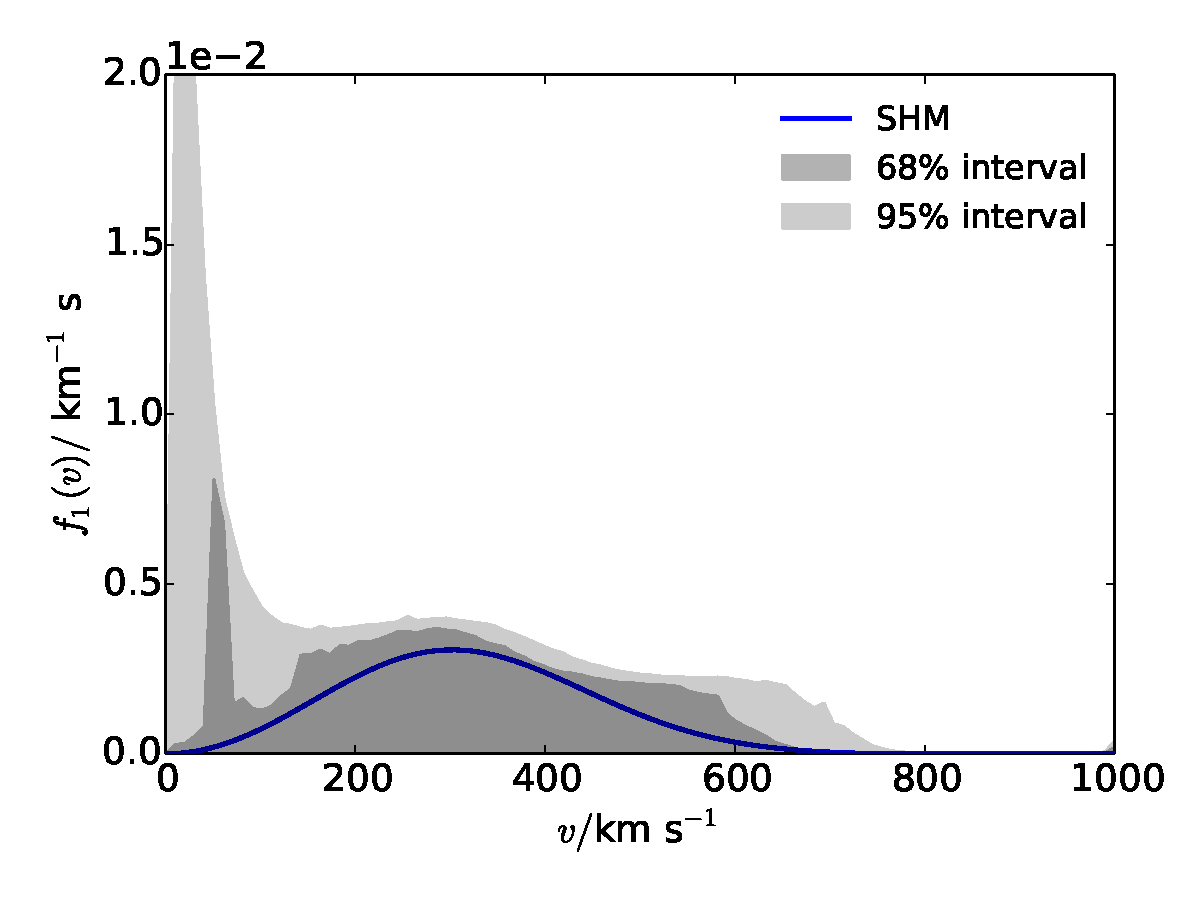
\includegraphics[width=0.75\textwidth]{Poly/f_SHM.pdf}
  \caption[Reconstructed speed distribution for a single realisation of data using the polynomial $\ln f(v)$ parametrisation]{Reconstructed speed distribution for a single realisation of data, generated for a 50 GeV WIMP. 68\% and 95\% credible intervals are shown as dark and light shaded regions respectively, while the underlying SHM distribution function is shown as a solid blue line. Reproduced from Ref.~\cite{Kavanagh:2014}.}
  \label{fig:Poly:f}
\end{figure}


This method performs poorly because, as initially mentioned in Sec.~\ref{sec:Poly:results}, we have no information about the fraction of dark matter particles below the energy threshold of our experiments. Varying $f_1(v)$ will change this fraction. There is thus a degeneracy between the shape of the speed distribution and the cross-section, meaning that we can only probe the shape of $f_1(v)$, rather than its overall normalization. This degeneracy has not been accounted for in Fig.~\ref{fig:Poly:f}. We can attempt to correct for this by adjusting the normalization of $f_1(v)$. If we fix $f_1(v)$ to be normalized to unity above $v_a$ (where $v_a \approx 171 \kms$ is the lowest speed probed by the experiments for a WIMP of mass 50 GeV), we can compare the shapes of the underlying and reconstructed distribution functions. This is illustrated in Fig.~\ref{fig:Poly:f_scaled}, which shows that we now broadly reconstruct the correct shape of $f_1(v)$. Below $v_a$, the value of $f_1(v)$ is poorly constrained, because the experiments provide no information about the shape of the distribution below theshold.

There remain several issues with this approach. In order to utilize this method, we must know the approximate value of the lowest speed probed by the experiments. However, this value is set by the WIMP mass. We could determine $v_a$ using the reconstructed WIMP mass, but this would be subject to significant uncertainty. In addition, direct reconstructions of the speed distribution may be easily biased. The upper limit of the energy windows of the experiments corresponds to a particular WIMP speed (for a given WIMP mass). WIMPs above this speed still contribute to the total event rate, but contribute no spectral information. The reconstructed shape of the high speed tail of the distribution is therefore not constrained by the data, but may affect the reconstructed value of $f_1$ at lower speeds.


\begin{figure}[t]
\centering
  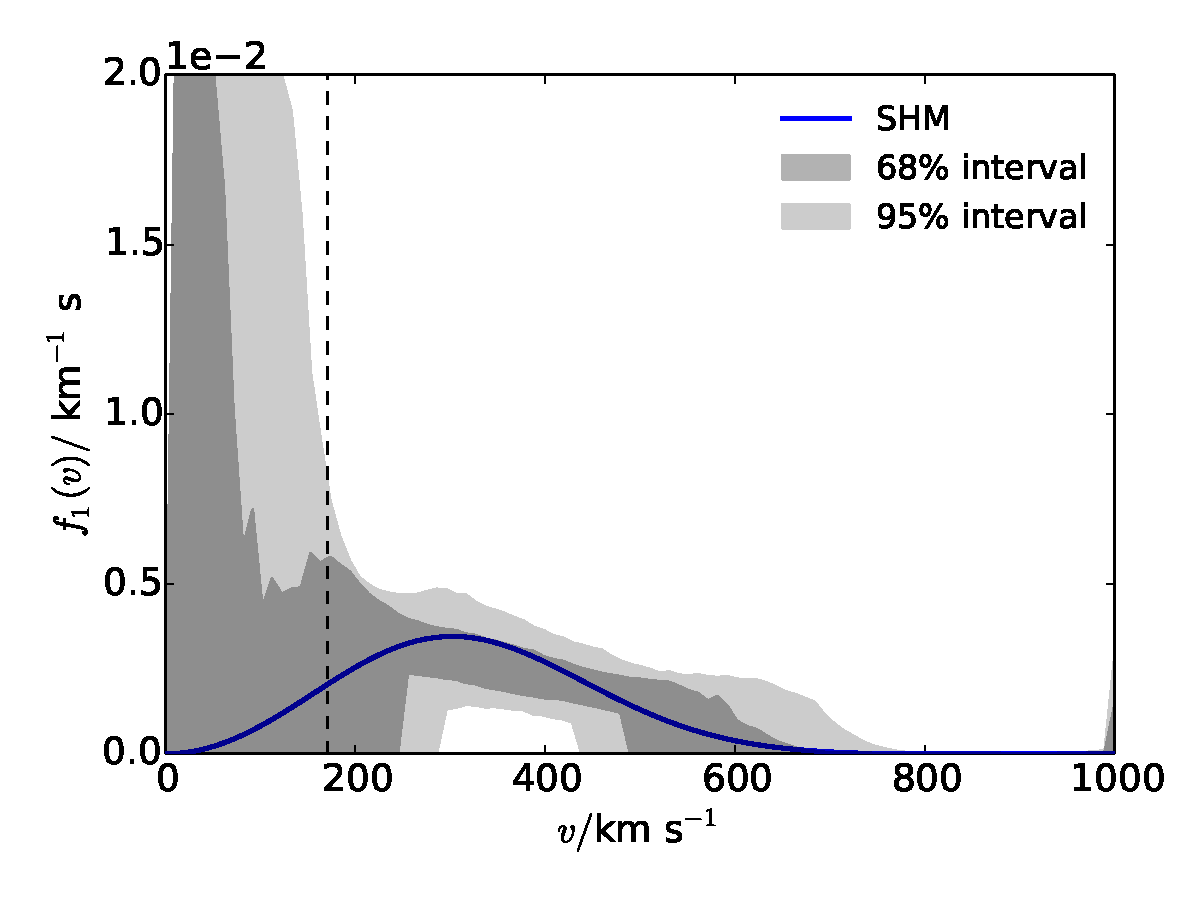
\includegraphics[width=0.75\textwidth]{Poly/f_SHM_scaled_line.pdf}
  \caption[Reconstructed speed distribution for a single realisation of data using the polynomial $\ln f(v)$ parametrisation, normalised to unity above the threshold speed of the experiments]{Reconstructed speed distribution for the same realisation of data as Fig.~\ref{fig:Poly:f}. In this case, we have also normalized $f_1(v)$ to unity above $v_a \approx 171 \kms$ (vertical dashed line). This is the lowest speed accessible to the experiments for a WIMP of mass 50 GeV. 68\% and 95\% credible intervals are shown as dark and light shaded regions respectively, while the underlying SHM distribution function is shown as a solid blue line. Reproduced from Ref.~\cite{Kavanagh:2014}.}
  \label{fig:Poly:f_scaled}
\end{figure}

An alternative approach is to reconstruct the mean inverse speed $\eta(v)$ (defined in Eq.~\ref{eq:DD:eta}) at some speed $v$. Because $\eta(v)$ is an integral function of $f_1$, it is less prone to bias as it takes into account the full shape of the distribution at speeds greater than $v$. However, we do not know the normalization of $f_1$ and so we must normalize $\eta$ appropriately. For each point sampled from $P(\textbf{a})$, we calculate $\eta$. We then divide by $\alpha(v)$, the fraction of WIMPs above speed $v$, calculated using the same parameter point:
\begin{equation}
\label{eq:alpha}
\alpha(v) = \int_{v}^{\infty} f_1(v') \, \textrm{d}v'\,.
\end{equation}

We will write this rescaled mean inverse speed as $\eta^*(v) = \eta(v)/\alpha(v)$. The value of $\eta^*(v)$ is a measure of the shape of the distribution function above $v$. However, some information about the normalization of the distribution has been factored out by dividing by $\alpha(v)$. We no longer need to know the value of $v_a$ in order to obtain information about the shape of the distribution at higher speeds. We may still need to decide the speed down to which we trust our reconstruction, but this no longer relies on an arbitrary choice of $v_a$ to normalize the reconstructions at all speeds.

In Fig.~\ref{fig:Poly:eta_stats}, we plot the mean reconstructed value of $\eta^*$ at several values of $v$, using 250 realisations of the 50 GeV SHM benchmark. We also show the mean upper and lower limits of the 68\% credible intervals as errorbars. The form of $\eta^*$ for the SHM is shown as a solid blue line. In all cases except for $v=100 \kms$, the mean reconstructed value is close to the true value, indicating that $\eta^*$ can be reconstructed without bias using this method. At low speeds, the reconstructed value deviates from the true value. In addition, the credible intervals lead to \textit{under}coverage in the $v=100 \kms$ case. However, this point lies below the lowest speed to which the experiments are sensitive and therefore we cannot trust the reconstruction at this low speed. We have checked that for the remaining values of $v$ the method provides exact or overcoverage, indicating that at higher speeds we can use $\eta^*$ as a reliable and statistically robust measure of the shape of the distribution.

\begin{figure}[t]
\centering
  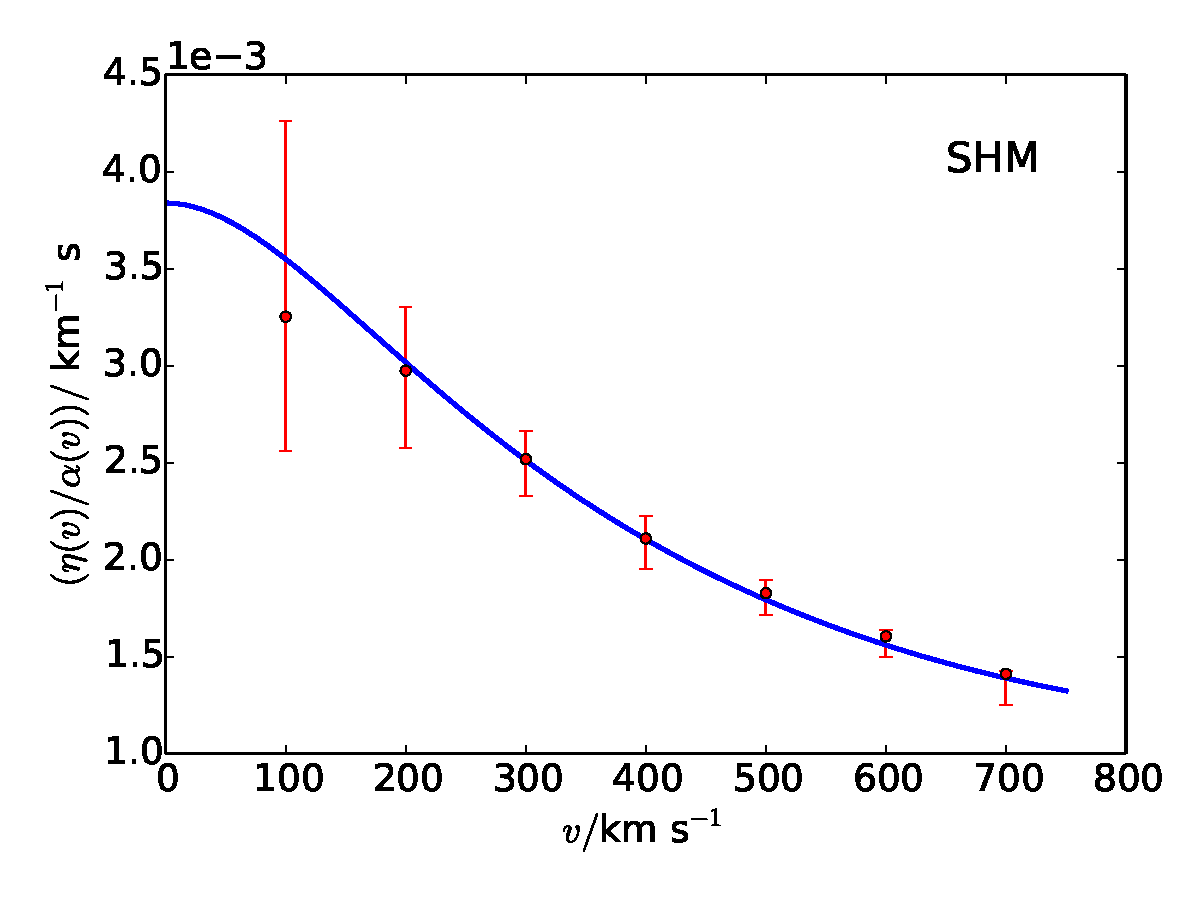
\includegraphics[width=0.75\textwidth]{Poly/Eta.pdf}
  \caption[Mean reconstructed values of the rescaled mean inverse speed over 250 realisations for a 50 GeV WIMP with SHM distribution function]{Mean reconstructed values of the rescaled mean inverse speed $\eta(v)/\alpha(v)$ at several values of $v$, calculated over 250 realisations of data using a 50 GeV WIMP and underlying SHM distribution function. Errorbars indicate the mean upper and lower limits of the 68\% credible intervals. The underlying form of $\eta(v)/\alpha(v)$ obtained from the SHM is shown as a solid blue line. Reproduced from Ref.~\cite{Kavanagh:2014}.}
  \label{fig:Poly:eta_stats}
\end{figure}


In the case of a single realisation of data, we would like to compare the probability distribution for $\eta^*(v)$ (obtained from $P(\textbf{a})$) to the value calculated from some test distribution. We note that several distributions may produce the same value of $\eta^*(v)$ at a given value of $v$. Thus, we may fail to reject a distribution function which is not the true distribution. However, if the calculated value of $\eta^*(v)$ does lie outside the $p\%$ interval, we can reject it at the $p\%$ level.

We can increase the discriminating power of this method by repeating this reconstruction over all speeds and checking to see if the benchmark value of $\eta^*$ is rejected at any value of $v$. The result of this procedure is shown in Fig.~\ref{fig:Poly:eta} for a single realisation of data generated using an SHM distribution (the same data as in Figs. \ref{fig:Poly:f} and \ref{fig:Poly:f_scaled}). We plot the 68\%, 95\% and 99\% credible intervals as shaded regions, as well as the values of $\eta^*(v)$ calculated from several benchmark speed distribution. We will focus on the intermediate speed range ($v \gtrsim 200 \kms$), as we do not know \textit{a priori} the lowest speed to which the experiments are sensitive.


\begin{figure}[t]
\centering
  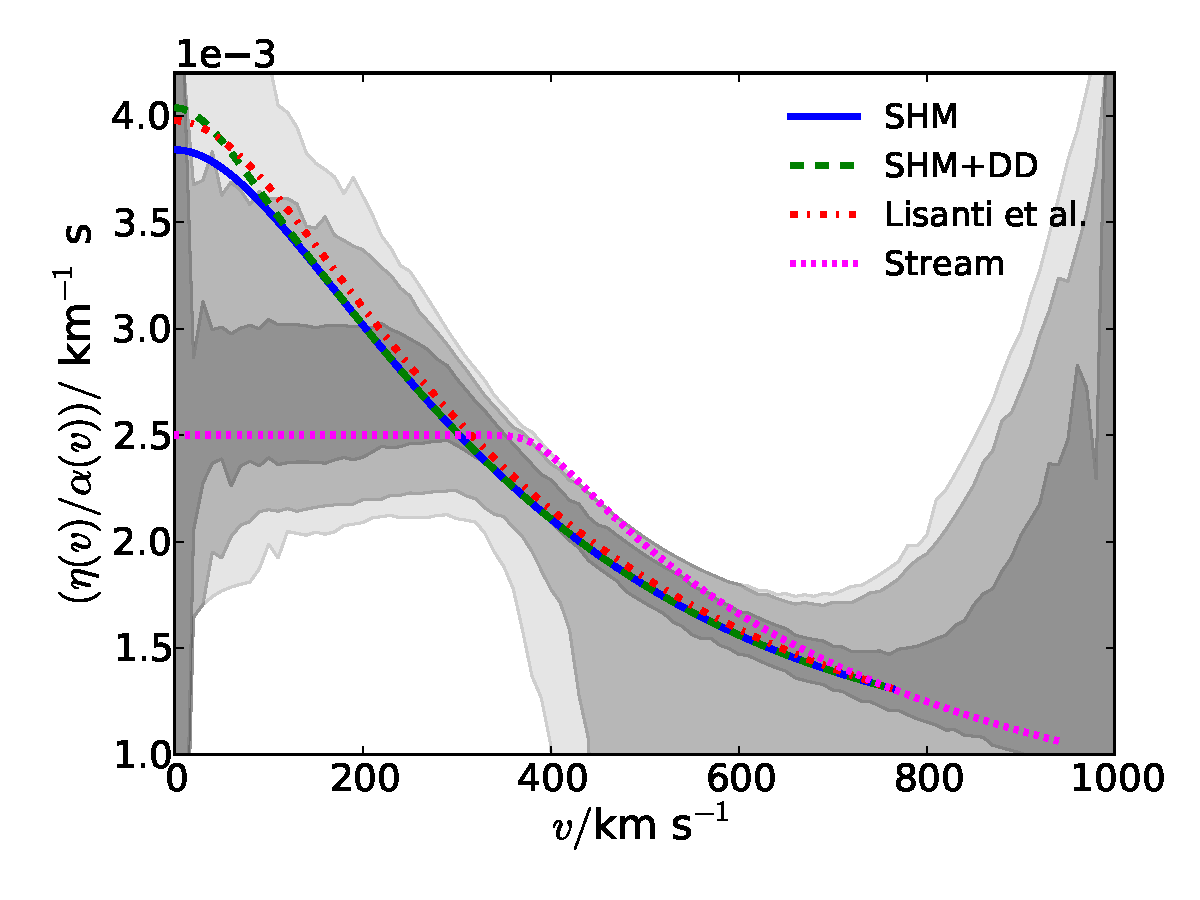
\includegraphics[width=0.75\textwidth]{Poly/SHM_lores.pdf}
  \caption[Rescaled mean inverse speed for a single realisation of data for a 50 GeV WIMP with SHM distribution function, showing several benchmark speed distributions for comparison]{Rescaled mean inverse speed $\eta(v)/\alpha(v)$, reconstructed from a single realisation of data using a 50 GeV WIMP and underlying SHM distribution function. At each value of $v$ we calculate 68\%, 95\% and 99\% credible intervals (shown as shaded intervals). We also show the calculated values of $\eta(v)/\alpha(v)$ for several possible benchmark speed distributions: SHM (solid blue), SHM+DD (dashed green), Lisanti et al.\ (dot-dashed red) and stream (dotted magenta). The benchmark curves are truncated when the underlying distribution function goes to zero. Reproduced from Ref.~\cite{Kavanagh:2014}.}
  \label{fig:Poly:eta}
\end{figure}

The reconstructed intervals are consistent with a range of possible distribution functions. The SHM and SHM+DD distributions are identical over a wide range of speeds. This is because above $\sim 200 \kms$, the two distributions differ in normalization but not in shape. Differences appear between the two at low speeds where their shapes diverge. The Lisanti et al.\ distribution results in a larger deviation from the SHM, but not sufficiently large to differentiate between the two distributions given the size of the uncertainties. Finally, the stream distribution results in a significantly different form for $\eta^*(v)$. At approximately $400 \kms$, the curve for the stream distribution lies outside the reconstructed 99\% credible interval. We can therefore use this method to reject the stream distribution at the 99\% confidence level.

Figure \ref{fig:Poly:eta_hires} shows the results of a reconstruction using a larger exposure. In this case, we generate data using the Lisanti et al.\ distribution and an exposure increased by a factor of $2.5$, resulting in approximately 1000 events across the three detectors. As expected, the resulting credible intervals are now substantially narrower. The stream distribution now lies significantly outside the 99\% interval. In Fig.~\ref{fig:Poly:eta_hires_zoom}, we show the same results, but focusing in on the region around $v \sim 400 \kms$. At certain points, the SHM and SHM+DD distributions now lie outside the 95\% credible interval, suggesting that with a number of events of the order of 1000, we may be able to reject these benchmarks.

\begin{figure}[t]
\centering
  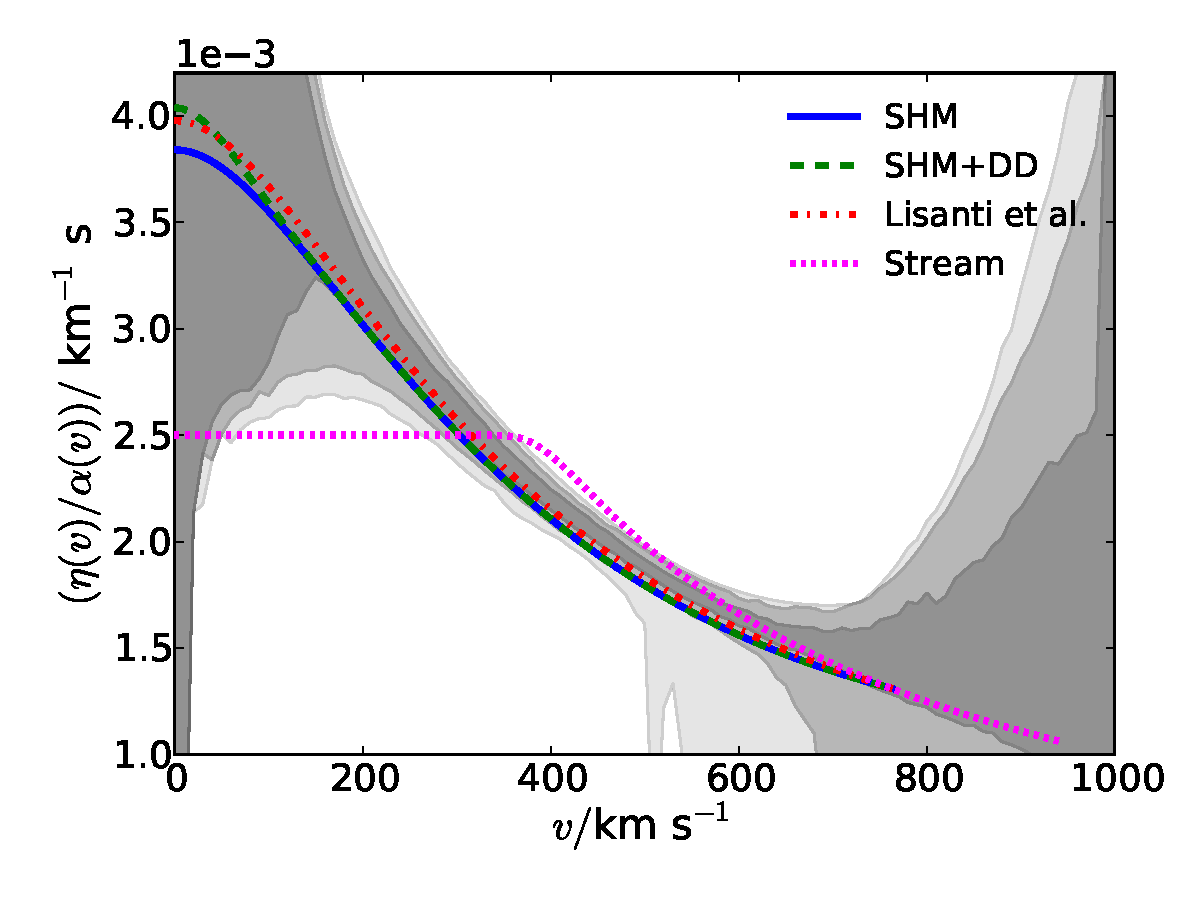
\includegraphics[width=0.75\textwidth]{Poly/LIS_hires.pdf}
  \caption{As Fig.~\ref{fig:Poly:eta}, but using as input a Lisanti et al.\ speed distribution and an exposure time which is 2.5 times longer. Reproduced from Ref.~\cite{Kavanagh:2014}.}
  \label{fig:Poly:eta_hires}
\end{figure}


\begin{figure}[t]
\centering
  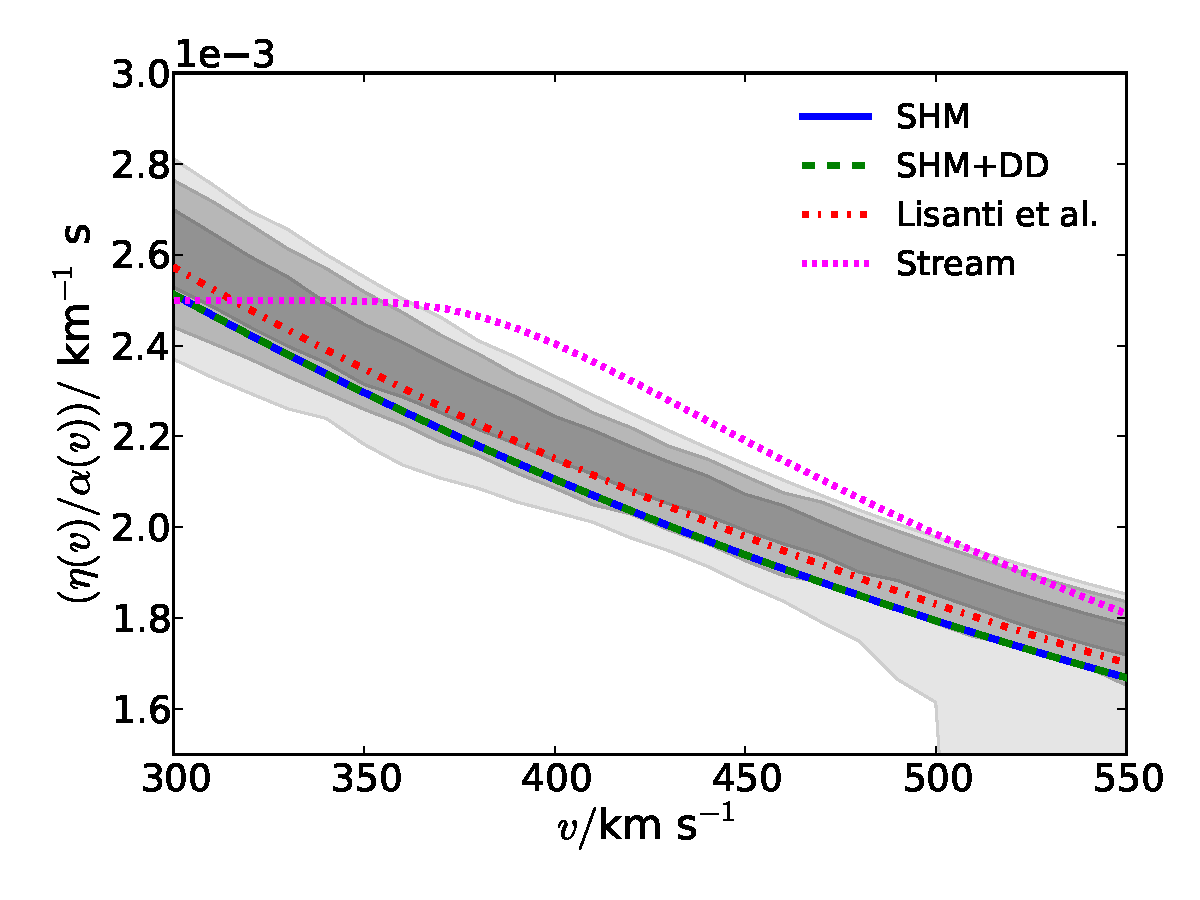
\includegraphics[width=0.75\textwidth]{Poly/LIS_hires_zoom.pdf}
  \caption[As Fig.~\ref{fig:Poly:eta_hires}, but focusing on the region around $v \sim 400 \kms$.]{As Fig.~\ref{fig:Poly:eta_hires}, but focusing on the region around $v \sim 400 \kms$. Notice that in the range $400-550 \kms$, both the SHM and SHM+DD curves lie at or below the lower limit of the 95\% credible interval. Reproduced from Ref.~\cite{Kavanagh:2014}.}
  \label{fig:Poly:eta_hires_zoom}
\end{figure}

While the method displayed in Fig.~\ref{fig:Poly:f_scaled} allows the approximate shape of the speed distribution to be reconstructed, reconstructions of $\eta^*(v)$ allow more statistically robust statements to be made about the underlying speed distribution. In particular, Fig.~\ref{fig:Poly:eta_hires_zoom} illustrates that with larger exposures deviations from Maxwellian speed distributions can be detected in a model-independent fashion.

\section{Discussion}

\todo{Is it worth having a comparison between this method and the speed binning and momentum binning methods? As in showing a table where I reconstruct the WIMP mass using all three? And then explain why (and in what ways) this one works better.}

\section{Conclusions}
\label{sec:Poly:conclusions}


We have studied in detail a new parametrization for the local dark matter speed distribution. This method involves writing the logarithm of the speed distribution as a polynomial in speed $v$ and fitting the polynomial coefficients (along with the WIMP mass and cross section) to the data. We have attempted to disentangle in this paper the influence of  different benchmark speed distributions, different benchmark WIMP masses and different forms for the parametrization. 

We have shown how the number of basis functions in the parametrisation can be chosen in a systematic way by minimising the Bayesian Information Criterion. We have also shown that the results are insensitive to the precise choice of basis functions, but that the Chebyshev polynomials can be used to efficiently explore the parameter space and result in a faster reconstruction than other choices. 

We have demonstrated that the WIMP mass can be reconstructed without bias in this method, using values in the range 10-500 GeV to test this. The inclusion of more realistic experimental uncertainties reduces the precision of the reconstructions, but does not introduce any bias. We have further tested the statistical properties of the WIMP mass reconstructions and have shown them to be robust over a range of possible speed distributions.

 We have presented several ways of displaying the reconstructed WIMP speed distribution using this method. In order to make robust statistical inferences about the speed distribution, we calculate the probability distribution of $\eta(v)/\alpha(v)$. This is the mean inverse speed $\eta(v)$, rescaled by the fraction of WIMPs $\alpha(v)$ above speed $v$. This can be used as a measure of the \textit{shape} of the distribution function, from which the unknown normalization has been factored out. We can then compare to the expected value of $\eta(v)/\alpha(v)$ from a given benchmark speed distribution, allowing us to distinguish between different underlying models.

Unfortunately, due to the finite threshold energies of direct detection experiments, we cannot probe the low speed population of WIMPs. If we make no assumptions, we have no information about the form of $f(v)$ below threshold and therefore little information about the overall normalisation of $f(v)$. This translates to an unavoidable degeneracy in the WIMP interaction cross section \sigmapsi. In spite of this, the completely general parametrisation presented in this Chapter can be used both to reconstruct the WIMP mass and probe the shape of the speed distribution in an unbiased and robust way.



\chapter[Neutrino telescopes]{Breaking the cross section degeneracy: neutrino telescopes}
\label{ch:NT}

The presence of dark matter (DM) in the Solar neighbourhood provides the opportunity to directly detect its scattering in terrestrial detectors. This may give us a handle on both the DM mass and speed distribution, providing we use a range of detector materials, as we have investigated in Chapter \ref{ch:Poly}. However, the finite energy thresholds of direct detection experiments means that we cannot probe the entire range of DM speeds. With no sensitivity to low speed WIMPs, we also cannot know what fraction of WIMPs are probed by the experiments, resulting in a loss of sensitivity to the DM interaction cross section.

The local DM population may also scatter with nuclei in the Sun, becoming gravitationally captured if enough energy is lost in the interaction \cite{Press:1985,Silk:1985, Gaisser:1986, Srednicki:1987, Griest:1987}. These can then annihilate in the Sun and produce neutrinos, which may be observed at neutrino telescope (NT) experiments such as IceCube. Importantly, capture occurs preferentially for WIMPs with low energy or, equivalently, low speed. Such a signal at a NT experiment would provide complementary sensitivity to the low speed WIMP population, hopefully breaking the degeneracy in the DM interaction cross section. 

In this chapter, we discuss the formalism for calculating the solar capture rate, as well as the processes of neutrino production, propagation and detection. We then test the binned speed parametrisation (discussed in Chapter \ref{ch:Speed}) and the polynomial parametrisation (presented in Chapter \ref{ch:Poly}) using both direct detection and IceCube mock data. In particular, we test the ability of these data sets - in conjunction with parametrisations of the speed distributions - to constrain the DM interaction cross sections in addition to the DM mass. We note that due to the high abundance of spin-1/2 hydrogen in the Sun, we must consider both spin-independent (SI) and spin-dependent (SD) couplings.

In Sec.~\ref{sec:NT:formalism}, we describe the IceCube event rate formalism. We then propose several particle physics and astrophysical benchmarks for the dark matter population in Sec.~\ref{sec:NT:benchmarks}. Section~\ref{sec:NT:experiments} describes the experimental parameters used in the analysis, with particular attention to the isotopic composition of detectors and the SD form factors. In the remaining sections, we consider reconstructions of particle physics parameters first without IceCube data (Sec.~\ref{sec:NT:withoutIC}) and then with IceCube data (Sec.~\ref{sec:NT:withIC}), before discussing the prospects for reconstructing $f(v)$ itself (Sec.~\ref{sec:NT:speeddist}).

\section{Neutrino telescope formalism}

Calculation of the expected spectrum of neutrinos at an NT experiment can be broadly decomposed into 3 contributions. The first is the rate at which WIMPs scatter and are captured in the Sun. The second is the subsequent thermalisation of the solar WIMP population and their eventual annihilation into neutrinos. Third, we must model the detection of neutrinos at the IceCube detector. We now consider each of these in turn, focusing on the first, as this is where the WIMP cross sections and speed distribution enter into the calculation.

\subsection{Solar capture}

In calculating the solar capture rate, we follow closely the treatment of Gould \cite{Gould:1987,Gould:1992}. WIMPs are captured by the Sun when they elastically scatter off one of its constituent nuclei and end up with a speed lower than the solar escape velocity (which at the surface is equal to \(v_{\textrm{esc}}^\odot = 617.5 \kms\) \cite{Kaufmann:1991}). These WIMPs then enter bound orbits intersecting the Sun, ensuring further scatters with solar nuclei during subsequent passes. WIMPs may become unbound in subsequent scatters (this possibility will be discussed later) but typically lose energy until they collect and thermalise around the Sun's core.

\begin{figure}[h!]
    \centering
    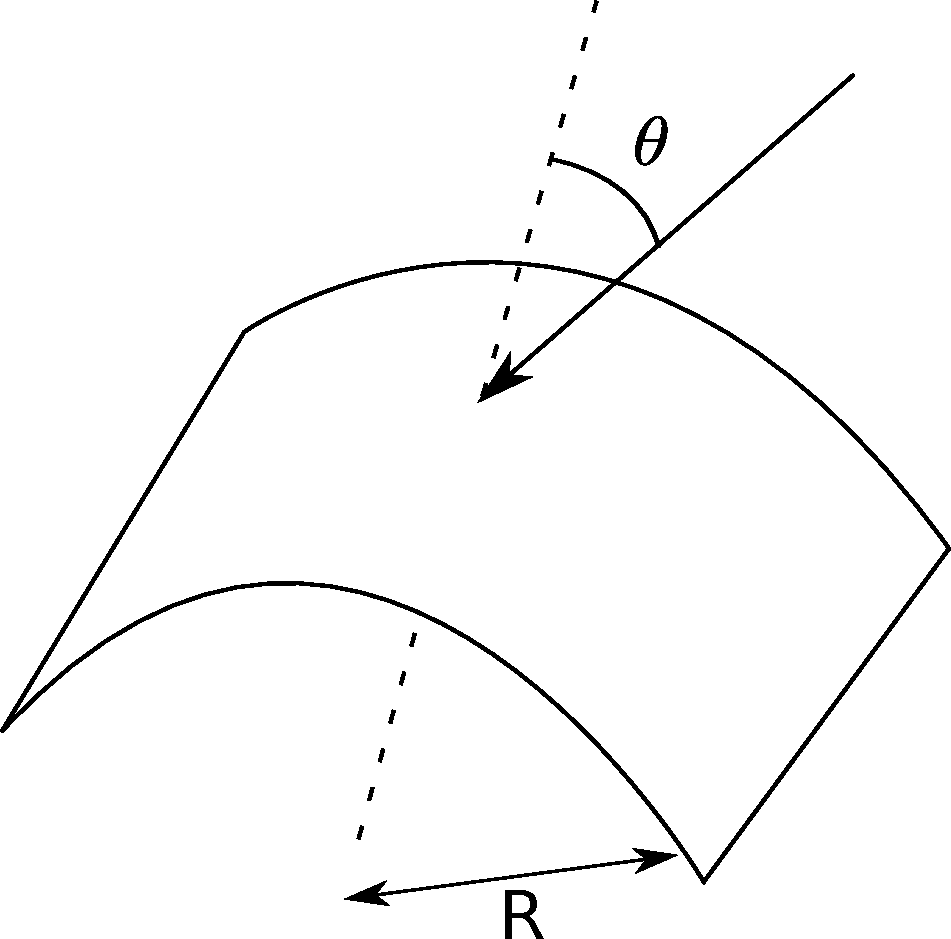
\includegraphics[width=0.4\textwidth]{NT/Surface.pdf}
\caption[Geometry of WIMPs impinging on the Sun]{Illustration of the geometry of WIMPs impinging on the Sun}
\label{fig:NT:geometry}
\end{figure}

In order to calculate this `first-scatter' probability, we consider a thin spherical shell of radius $R$, large enough that the gravitational field at $R$ is negligible. This geometry is illustrated schematically in Fig.~\ref{fig:NT:geometry}. The number density of WIMPs with speed $v$ is $n_\chi f_1(v) \,\mathrm{d}v$. Because of the spherical symmetry of the problem, we can assume that the WIMP velocity distribution is isotropic without loss of generality. The fraction of WIMPs with direction $\cos \theta \rightarrow \cos \theta + \textrm{d} \cos \theta$ relative to the perpendicular direction is $\frac{1}{2} \textrm{d}\cos\theta$ (normalised over all values of $\cos \theta$). The WIMP speed perpendicular to the surface is given by $v \cos\theta$, meaning that the WIMP flux inward through the surface (per unit area) can be written:
\begin{equation}
\frac{1}{2} f_1(v) v \cos\theta \,\textrm{d}v \,\textrm{d}\cos\theta = \frac{1}{4} f_1(v) v \,\textrm{d}v \,\textrm{d}\cos^2\theta \,, \qquad \theta \in [0, \frac{\pi}{2}]\,.
\end{equation}
We change variables to angular momentum per unit mass, $ J = R v \sin\theta $, and integrate over all area elements on the surface of the shell to obtain the inward WIMP flux per unit time
\begin{equation}
4 \pi R^2 \frac{1}{4}f_1(v) v \, \textrm{d}v \frac{\textrm{d}J^2}{R^2 v^2}.
\end{equation}

\note{[***Missing a factor of the WIMP density***]}
We now consider an inner shell of radius $r$ and thickness $dr$. If the escape velocity at the shell is $\vesc(r)$, then a WIMP with speed $v$ at infinity will have speed $w = \sqrt{v^2 + \vesc^2(r)}$ at this inner shell. The total time the WIMP spends in the shell is

\begin{equation}
\frac{\textrm{d}l}{w} = \frac{2}{w \cos \theta} \Theta(1 - \sin\theta) \, \textrm{d}r = \frac{2}{w}\left[ 1 - \left(\frac{J}{rw}\right)^2\right]^{-1/2} \Theta(rw - J) \, \textrm{d}r\,,
\end{equation}
where the Heaviside step function $\Theta$ appears because the WIMP crosses the shell either twice or not at all. If the rate per unit time at which a single WIMP travelling at velocity \(w\) is scattered down to a speed less than the escape speed \(\vesc\) is given by \(\Omega^{-}_{\vesc,i}(w)\), then we can write the WIMP capture rate per unit time per unit velocity as
\begin{align}
&2\pi \, \textrm{d}r \frac{f_1(v)}{v}\,\textrm{d}v \frac{\ScatRate}{w}  \, \int_{0}^{(rw)^2} \left[ 1 - \left(\frac{J}{rw}\right)^2\right]^{-1/2} \, \textrm{d}(J^2) \nonumber\\&\qquad= 4 \pi r^2 \, \textrm{d}r \frac{f_1(v)}{v}\, \textrm{d}v w \ScatRate\,.
\end{align}

The `first scatter' rate is then given by integrating over the radius of the Sun:
\begin{equation}
C_{\odot} = \frac{\rho_0}{m_\chi} \int_{0}^{R_{\odot}} \textrm{d}r \sum_i \dbd{C_i}{V} 4 \pi r^{2},
\end{equation}
where the capture rate per unit shell volume is
\begin{equation}
\label{eq:NT:dCdV}
\dbd{C_i}{V} = \int_{0}^{v_{\textrm{max}}} \textrm{d}v \frac{f_1(v)}{v} w \ScatRate\,.
\end{equation}
The index \(i\) labels the various nuclei in the Sun. The integration limit is
\begin{equation}
v_{\textrm{max}} = \frac{\sqrt{4m_\chi m_{N_i}}}{m_\chi - m_{N_i}}\vesc\,.
\end{equation}
WIMPs above this speed cannot lose enough energy in a recoil to drop below the escape speed.

We now calculate the factor $\ScatRate$, which gives the rate per unit time at which a single WIMP travelling at velocity \(w\) is scattered down to a speed less than the escape speed \(\vesc\). This rate can be written as:
\begin{equation}
\ScatRate = \Phi_\chi N_T \sigma_{\vesc}\,
\end{equation}
where \(\Phi_\chi N_T\) is the WIMP flux multiplied by the number of target nuclei. For a single WIMP and a number density of nuclei \(n_N\), this becomes \( \Phi_\chi N_T = w n_N\). The cross-section for the process \(\sigma_{\vesc}\) is given by:
\begin{equation}
\label{eq:NT:sigma}
\sigma_{\vesc}  = \int_{E_{\vesc}}^{E_\textrm{max}} \dbd{\sigma}{E_R} \, \textrm{d}E_R\,
\end{equation}
where \(E_R = \Delta E\) is the energy lost by the scattering WIMP. The limits of integration run from the minimum energy loss required to reduce the WIMP speed below \vesc,
\begin{equation}
E_{\vesc} = \frac{m_\chi}{2}(w^2 - \vesc^2) = \frac{m_\chi}{2}v^2\,,
\end{equation}
to the maximum possible energy loss in the collision,
\begin{equation}
E_\textrm{max} = \frac{2 \mu_{\chi N}^2}{m_N} w^2\,.
\end{equation}

As in the direct detection case, we can decompose the differential cross section into SI and SD components. While all of the constituent elements of the Sun are sensitive to the SI interaction, only spin-1/2 Hydrogen is sensitive to SD scattering. The differential cross section is therefore given by

\begin{equation}
\dbd{\sigma}{E_R} = \frac{m_{N_i}}{2\mu_{\chi p}^2 v^2}
\begin{cases}
\sigmapsi + \sigmapsd & \textrm{ for } A = 1 \\
\sigmapsi A_i^2 F_i^2(E_R) & \textrm{ for } A > 1 \,.
\end{cases}
\end{equation}
No form factor is needed for Hydrogen ($A=1$), which consists of only a single nucleon. For the remaining nuclei, approximate the form factor as \cite{Gould:1987}
\begin{equation}
F^2_i(E_R) = \exp(-E_R/E_i); \qquad E_i = \frac{3}{2m_{N_i} R_i^2}\,,
\end{equation}
where $R_i$ is the nuclear radius (see Sec.~\ref{}). These expressions allow Eq.~\ref{eq:NT:sigma} to be calculated analytically and introduce an error in the total capture rate of only a few percent.

\note{Might need some plots illustrating capture rates...}

In addition to the effects which have already been described, we can also consider a number of other factors which may impact the WIMP capture rate. The fact that nuclei in the Sun have a finite temperature has been neglected so far. However, detailed calculation \cite{Press:1985,Gould:1987} shows that this gives a correction to the capture rate of only around 1\% for WIMP masses above around 10 GeV. The gravitational influence of other bodies in the Solar system may also have an impact. For example, Peter \cite{Peter:2009} found that WIMPs whose bound orbits reach out as far as Jupiter can be perturbed by the planet and become unbound. This leads to so-called \textit{Jupiter depletion} for WIMPs heavier than around 1 TeV. However, a recent study by Sivertsson and Edsj\"{o} \cite{Sivertsson:2012} showed using Liouville's theorem that such depletion processes must be accompanied by an inverse diffusion process. The net result is that for Solar capture we can treat the WIMP population as being free.

\note{Gould:1991}

\subsection{Evolution of the WIMP population}

Once a WIMP has scattered to below the escape speed at a given solar position, it will be in a bound orbit and will enter the population of WIMPs captured by the Sun. Subsequent scatters with the nuclei in the Sun will lead to an approximately thermal distribution. There are then two processes which will tend to deplete this population: WIMP evaporation and annihilation. \note{Look up \cite{Krauss:1986}.} 

Evaporation occurs when WIMPs scatter into the high speed tail of the thermal distribution, above the Solar escape velocity, and become unbound. It has been shown that for a WIMP mass of around 4 GeV, the evaporation timescale is approximately equal to the lifetime of the Sun ($\sim4.7$ billion years) \cite{Gould:1987b}. For WIMPs significantly heavier than this, the evaporation rate is negligible compared to the capture rate. For WIMPs lighter than this, the tail of the Maxwell-Boltzmann distribution lying above the escape velocity becomes significant and evaporation can no longer be neglected \cite{Busoni:2013b}. As we will see, the IceCube detector is sensitive to WIMPs with masses above around $m_\chi > 20 \textrm{ GeV} $, meaning that we can safely ignore the effects of evaporation.

The population of WIMPs will also undergo annihilation (either with their anti-particle partners or with themselves if they are Majorana particles). The evolution of the total number $N(t)$ of WIMPs in the Sun can then be written as \cite{Griest:1987}:

\begin{equation}
\dbd{N}{t} = C_c - \frac{1}{2}C_a N^2 - C_e N\,.
\end{equation}
The parameter $C_c$ is the total capture rate and the parameters $C_a$ and $C_e$ determine the annihilation and evaporation rates. As we have discussed, we can safely negelect evaporation, so we set $C_e$ to zero. The parameter $C_a$ and therefore the annihilation rate will depend on the velocity-averaged annihilation cross section $\langle \sigma v \rangle$ which is \textit{a priori} unknown. Over a long period of time, equilibrium between the capture and annihilation will be achieved and a steady state scenario for the WIMP population will be reached. This timescale is set by the equilibration time $\tau = 1/\sqrt{C_c C_a}$. If this is sufficiently short compared to the lifetime of the Sun, the WIMP population will currently be in equilibrium with the annihilation rate $\Gamma_a$ set by the capture rate as

\begin{equation}
\Gamma_a = \frac{1}{2}C_a\,.
\end{equation}

Crucially, in this case, the annihilation rate no longer depends on the unknown annihilation cross section, but is related only to the WIMP-nucleus scattering cross sections. We will assume in the rest of this chapter that the annihilation cross section is sufficiently high that the equilibrium assumption is valid.

Standard Model (SM) particles are produced in these annihilations, the majority of which cannot escape the Sun. However, some of these particles may decay to neutrinos or neutrinos may be produced directly in the WIMP annihilation. These neutrinos can escape the Sun and may be detected at neutrino telescope experiments on Earth. It is important to account for the production and propagation of neutrinos in the dense medium of the Sun, as well as the propagation of these neutrinos from the Sun to the Earth \cite{Blennow:2008}. The spectrum of neutrinos reaching Earth can be written as \note{Wait but this doesn't take into account the propagation does it...?}

\begin{equation}
\dbd{N_\nu}{E_\nu} = \frac{\Gamma_a}{4\pi D^2}\sum_f B_f \dbd{N_\nu^f}{E_\nu}\,,
\end{equation}
where $D$ is the Earth-Sun distance, $\mathrm{d}N_\nu^f/\mathrm{d}E_\nu$ is the neutrino spectrum produced in the Sun for a particular final state $f$ and $B_f$ is the branching ratio into that final state. The branching ratios will depend on the specific form of the dark matter interactions with baryons. Typically, in order to set constraints on the WIMP interaction cross sections, we consider annihilation into only one channel at a time, assuming $B_f = 1$ for that particular channel during the analysis. Finally, the neutrino spectrum produced in the annihilation $\mathrm{d}N_\nu^f/\mathrm{d}E_\nu$ can be obtained using particle physics event generators (such as \textsc{Pythia} \cite{Sjostrand:1994}) and propagated to Earth using neutrino Monte Carlo simulations (such as WimpSim \cite{Blennow:2008}).


\note{Sub-section on propagation??? What should go in which section???}

\subsection{Detection}

Neutrinos which escape the Sun can be detected at terrestrial NT experiments \cite{Adrian-Martinez:2013,Aartsen:2013b}. We focus in this work on the IceCube experiment \cite{Aartsen:2013b}, which can detect the \v{C}erenkov radiation produced by high energy particles traveling through ice. Muon neutrinos interact via charged-current interactions in the ice to produce relativistic muons. These in turn produce \v{C}erenkov light, which is collected by digital optical modules (DOMs). The amount and pattern of lit DOMs allows the energy and direction of the incoming neutrino to be reconstructed \note{with varying degrees of accuracy}. 

\todo{Talk about showers vs cascades}

\todo{Talk about the energy threshold}

\todo{Talk about DeepCore! \cite{Abbasi:2012}} 

\todo{Talk about the event-level likelihoods paper... - base it on that!}

\section{Complementarity with direct detection}

The complementarity between direct detection and NT data has been studied in the past \cite{Arina:2013}. In particular, the high abundance of hydrogen can help to constrain the spin-dependent cross section and, even in cases where no signal is observed at IceCube, limits from NT experiments can help to reduce the size of the allowed parameter space. Here, we explore further this complementarity by looking at the range of speeds which are probed by NT experiments.

As can be from Eq.~\ref{eq:NT:dCdV}, WIMPs with speeds from $v=0$ up to $v=v_\textrm{max}$ have the possibility of being captured by the Sun. In particular, with increasing WIMP speed the capture probability decreases, \note{Not even sure if this is true}, further suppressed by loss of coherence in the SI case. As pointed out in Ref.~\cite{Choi:2013}, direct detection experiments probe a complementary range of the WIMP speed distribution, defined by the energy range of the WIMP search window. If the ranges of speeds probed by direct detection and NT experiments overlaps, this means that the entire WIMP speed distribution can be probed.

In Fig.~\ref{fig:NT:speedoverlap}, we show the WIMP speeds to which two experiments are sensitive as a function of WIMP mass. As a blue band, we show the region probed by a Xenon direction detection experiment. The lower and upper limits of the band are set by $v_\textrm{min}(\Emin)$ and $v_\textrm{min}(\Emax)$, where \Emin and \Emax define the extent of the WIMP signal window. In this chapter, we consider a window of $[5,45]$ keV \cite{}. WIMPs with speeds above the blue band still contribute to the overall event rate (so there is still some sensitivity to them). However, there is no information on the \textit{shape} of the distribution at higher speeds, as we are not sensitive to the event spectrum above \Emax.


\begin{figure}[t]
  \centering
  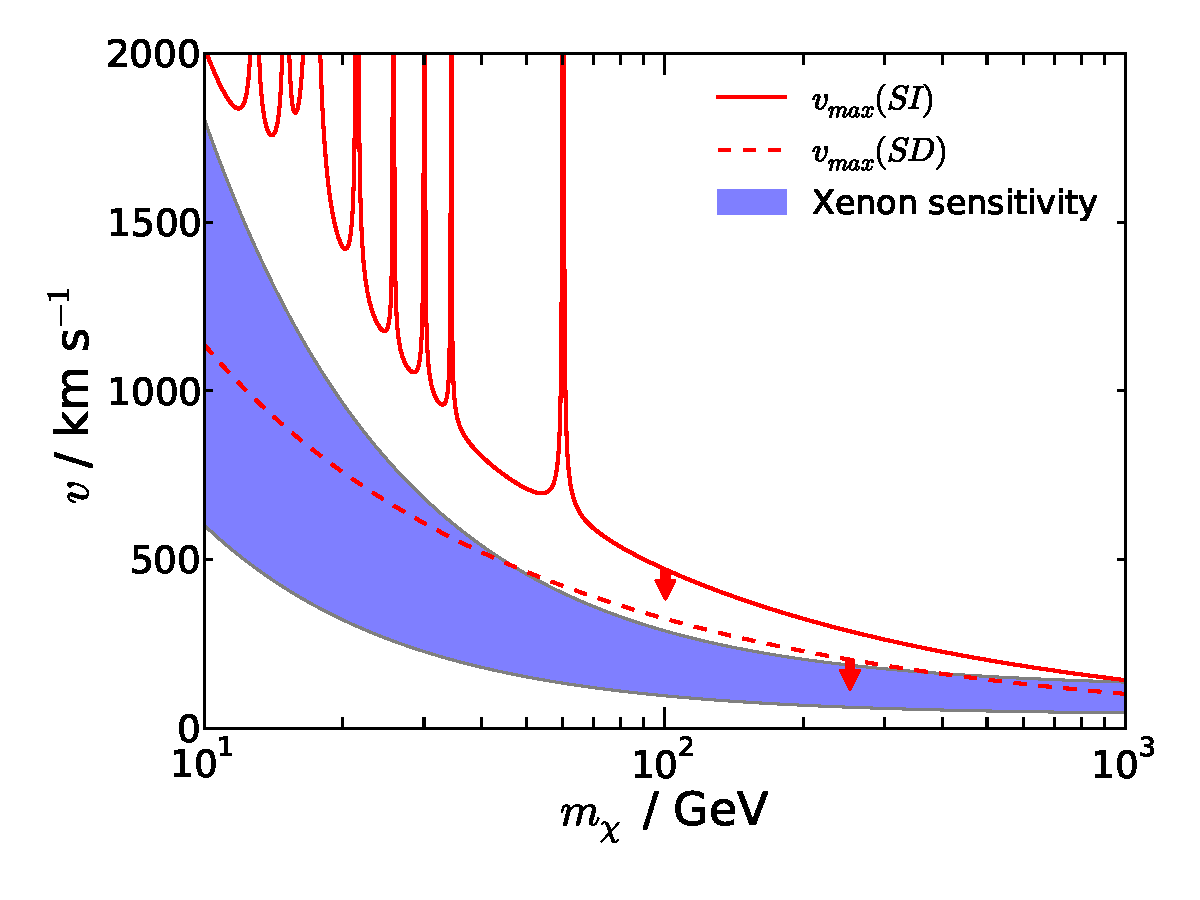
\includegraphics[trim=0.8cm 0.9cm 0cm 0cm, clip,width=0.75\textwidth]{NT/SpeedOverlap.pdf}
  \caption[Speed sensitivity ranges of solar capture and direct detection experiments as a function of WIMP mass]{Sensitivity ranges of solar capture and direct detection experiments. We show as a blue band the range of speeds to which a Xenon detector is sensitive using an energy window of $[5,45]$ keV. The maximum speed to which solar WIMP capture is sensitive is shown as a solid (dashed) red line for SI (SD) interactions (see the text for more details).}
  \label{fig:NT:speedoverlap}
\end{figure}

Also shown in Fig.~\ref{fig:NT:speedoverlap} are the values of $v_\textrm{max}$ involved in the Solar capture rate for SI and SD interactions. In the SD case, the maximum speed is set by the hydrogen mass $m_H$:

\begin{equation}
v_{\textrm{max}} = \frac{\sqrt{4m_\chi m_H}}{m_\chi - m_H}\vesc\,.
\end{equation}
The escape speed \vesc depends on radius within the Sun so we use an average value, weighted by the hydrogen density as a function of radius. In the SI case, the situation is more complex, as more than one nucleus contributes to the capture rate. We therefore consider the average value of $v_\textrm{max}$ weighted by the mass fraction $f_i$ of each species

\begin{equation}
\langle v_{\textrm{max}} \rangle = \sum_i f_i \frac{\sqrt{4m_\chi m_{N_i}}}{m_\chi - m_{N_i}}\vesc\,,
\end{equation}
where again \vesc is evaluated at the average radius of each species $i$.

In the SD case, the decreasing value of $v_\textrm{max}$ with $\mchi$ reflects the kinematics of the $\chi-H$ interaction. As the WIMP mass increases, scattering with hydrogen becomes less effecient at transferring energy. In the SI case, the value of $v_\textrm{max}$ is typically higher because the WIMP is closer in mass to the heavier nuclei in the Sun. However, there is still a significant SI interaction with hydrogen and the same decay with $\mchi$ is observed as in the SD case. In addition, there are resonances in $v_\textrm{max}$, corresponding to perfect mass matching between the WIMP and one of the nuclei in the Sun. In these cases, energy transfer is highly efficient and WIMPs of any speed can scatter into bound orbits.

The key point of Fig.~\ref{fig:NT:speedoverlap} is that in both the SI and SD dominated cases, $v_\textrm{max}$ never falls below the lower limit of the blue band. This means that the combination of NT and direct detection data should provide sensitivity to the full range of WIMP speeds over a range of masses. The level of sensitivity may vary with WIMP speed, due for example to a falling capture contribution from higher speeds or form factor suppression in direct detection experiments. However, in principle, we can probe the full WIMP speed distribution and hopefully break the degeneracy in the cross section described in Chapter~\ref{ch:Poly}. The inclusion of data sets from additional direct detection experiments should only improve this sensitivity.

\note{Need a linking paragraph here...}



\section{Current limits?}

\section{Benchmarks and experiments}
\label{sec:NT:experiments}
In order to test these parametrisations and determine how well the WIMP parameters can be recovered, we generate mock data sets for a set of hypothetical direct detection experiments as well as for IceCube. We show in Table~\ref{tab:NT:Experiments} the parameters used in this work for three direct detection experiments chosen to mimic next-generation detectors currently in development. Each experiment is described by the range of nuclear recoil energies it is sensitive to and the total exposure (the product of the fiducial detector mass, the exposure time and the experimental and operating efficiencies). We also include a gaussian energy resolution of $\sigma_E = 1 \textrm{ keV}$ and a flat background rate of $10^{-7}$ events/kg/day/keV.

\note{NB: `While the exact reconstructions, and in particular the uncertainties, will depend on the values used for the experiments and benchmarks, the general method is gooood.'}

We divide the energy range of each experiment into bins and generate Asimov data \cite{Cowan:2013} by setting the observed number of events in each bin equal to the expected number of events. While this cannot correspond to a physical realisation of data as the observed number of events will be non-integer, it allows us to disentangle the effects of Poisson fluctuations from the properties of the parametrisations under study.

\begin{table}[t]
  \setlength{\extrarowheight}{3pt}
  \begin{center}
%\begin{sideways}
	\begin{tabular}{cm{2.75cm}m{2.5cm}m{2.75cm}}
        \hline\hline
	Experiment & Energy Range (keV) & Exposure (ton-yr) & Energy bin width (keV) \\
        \hline
	Xenon &  5-45 & 1.0 & 2.0 \\
	Argon &  30-100 & 1.0 & 2.0 \\
	Germanium  & 10-100 & 0.3 & 2.0 \\
        \hline\hline
	\end{tabular}
%\end{sideways}
  \end{center}
\label{tab:NT:Experiments}
\caption[Summary of parameters for mock direct detection experiments used in Chapter~\ref{ch:NT}]{Summary of parameters for mock direct detection experiments. All experiments have a constant energy resolution of $\sigma_E = 1 \textrm{ keV}$ and a flat background rate of $10^{-7}$ events/kg/day/keV. \note{Probably need some references/justification for some of these values.}}
\end{table}

To generate neutrino telescope data, we consider the IceCube 86-string configuration. We use an exposure time of 900 days (corresponding to five 180 day austral winter observing seasons, as in Ref.~\cite{Arina:2013}). We use an angular cut around the solar position $\phi_\textrm{cut} = 3\,^{\circ}$. This results in approximately 217 background events over the full exposure. As with the direct detection experiments, we set the observed number of events equal to the expected number of signal plus background events. We use only the observed number of events as data and not the energies of the individual events. While event-level likelihood methods have previously been developed \cite{Scott:2012} for use with IceCube 22-string data \cite{Abbasi:2009}. However, a similar analysis has not been performed for IceCube-86. In particular, the probability distributions for the number of lit digital optical modules (DOMs) as a function of neutrino energy are not yet available for IceCube-86. Nonetheless, using the number of observed events at IceCube is a first step towards using neutrino telescope data to help constrain the WIMP speed distribution.

\subsection{Benchmarks}
\label{sec:NT:benchmarks}
We use four benchmark models to generate mock data sets, which are summarised in Table~\ref{tab:benchmarks}. In all cases, we use an SI WIMP proton cross section of $\sigmapsi = 10^{-45} \textrm{ cm}^2$ and SD cross-section of $\sigmapsd = 2 \times 10^{-40} \textrm{ cm}^2$, both of which are close to the current best exclusion limits \cite{Akerib:2014, Aprile:2013}. For simplicity, we assume that the WIMP-proton and WIMP-neutron couplings are equal in both the SI and SD cases. We could allow the ratio of these couplings to vary as free parameters, but this would introduce additional degeneracies into the analysis. Here we focus on the degeneracy associated with the WIMP speed distribution.

Benchmark A represents an intermediate mass WIMP which annihilates to $W^{+}W^{-}$, which is similar to benchmark B used by Ref.~\cite{Arina:2013}. As we will see, even with this intermediate mass there is already a strong degeneracy in the reconstructed WIMP mass. We therefore choose not to consider a benchmark model with higher mass, which would result in an even poorer sensitivity to the reconstructed WIMP mass. We do, however, consider a lighter WIMP in benchmark C, which annihilates to $\nu_\mu \bar{\nu}_\mu$. The IceCube detector (with DeepCore) is sensitive to WIMPs with masses down to about 20 GeV \cite{}. We therefore use a 30 GeV WIMP mass, as WIMPs much lighter than this cannot feasibly be detected by IceCube.

\begin{table*}[t]
  \setlength{\extrarowheight}{3pt}
  \begin{center}
%\begin{sideways}
	\begin{tabular}{ccccccc}
        \hline\hline
	Benchmark & $m_\chi \textrm{ (GeV)}$ & $\sigma^p_{SI} \textrm{ (cm}^2\textrm{)}$ & $\sigma^p_{SD} \textrm{ (cm}^2\textrm{)}$ & Speed distribution & Decay channel \\
	\hline
        A & 100 & $10^{-45}$ & $2 \times 10^{-40}$ & SHM & $W^{+}W^{-}$ \\
        B & 100 & $10^{-45}$ & $2 \times 10^{-40}$ & SHM+DD & $W^{+}W^{-}$ \\
        C & 30  & $10^{-45}$ & $2 \times 10^{-40}$ & SHM & $\nu_\mu \bar{\nu}_\mu$ \\
        D & 30  & $10^{-45}$ & $2 \times 10^{-40}$ & SHM+DD & $\nu_\mu \bar{\nu}_\mu$ \\
        \hline\hline
	\end{tabular}
%\end{sideways}
  \end{center}
\label{tab:NT:benchmarks}
\caption[Summary of benchmarks used in Chapter~\ref{ch:NT}]{Summary of benchmarks. In all cases, we consider only isospin conserving interactions (i.e. $f_p = f_n$ and $a_p = a_n$).}
\end{table*}

Benchmarks A and C assume an SHM speed distribution described by $v_\textrm{lag} = 230 \kms$ and $\sigma_v = 163 \kms$. Benchmarks B and D assume the same particle physics parameters as A and C respectively, but assuming an SHM distribution with a moderate dark disk overdensity (SHM+DD). We model the dark disk as contributing an additional 30\% dark matter density to the SHM, with parameters $v_\textrm{lag} = 50 \kms$ and $\sigma_v = 50 \kms$ \cite{}. As shown in Ref.~\cite{Choi:2013}, the capture rate in the Sun is not strongly dependent on variations in the shape of $f(v)$ (such as the differences between distribution functions extracted from different N-body simulations). However, significant enhancement of the capture rate can be achieved with the presence of a low speed dark disk, which we investigate using these two astrophysical benchmarks.

%%%%%Hmmm...the speed distribution probed by the earth is not precisely the same as the one probed by the Sun because of the Earth's motion round the Sun...but that's not a big factor

\subsection{Parameter sampling}
\label{sec:NT:sampling}
We perform parameter scans using a modified version of the publicly available \textsc{MultiNest 3.6} package \cite{Feroz:2007, Feroz:2008, Feroz:2014}. This allows us to map out the likelihood $\mathcal{L}(\theta)$ for the model parameters $\theta$.  We use $N_\textrm{live} = 20000$ live points in the scans and a tolerance of $10^{-4}$. We show in Table~\ref{tab:NT:priors} the priors on the various model parameters used in this work.

\begin{table}
  \setlength{\extrarowheight}{3pt}
  \begin{center}
%\begin{sideways}
	\begin{tabular}{ccc}
        \hline\hline
	Parameter & Prior range & Prior type \\
        \hline
        $m_\chi$ (GeV) & 10-1000 & log-flat \\
        $\sigma^p_{SI} \textrm{ (cm}^2\textrm{)}$ & $10^{-48} - 10^{-42}$ & log-flat \\
        $\sigma^p_{SD} \textrm{ (cm}^2\textrm{)}$ & $10^{-43} - 10^{-37}$ & log-flat \\
        Polynomial coefficients $\left\{a_k\right\}$ & $-20 - 20$ & linear-flat \\
        Bin heights $\left\{\hat{g}_k\right\}$ & $0-1$ & simplex \\
        \hline\hline
        \end{tabular}
%\end{sideways}
  \end{center}
\label{tab:NT:priors}
\caption[Summary of \textsc{MultiNest} priors used in Chapter~\ref{ch:NT}]{Summary of \textsc{MultiNest} priors used in this work. The `simplex' priors are described in Sec.~\ref{sec:sampling}.}
\end{table}

\note{Need to actually mention/include something about the parametrisations in this chapter...}
Due to the normalisation condition on the bin heights (given in Eq.~\ref{eq:normalisation}), we must sample these parameters from `simplex' priors. That is, we must uniformly sample $\left\{\hat{g}_2,...,\hat{g}_N\right\}$ such that they sum to less than one and then fix $\hat{g}_1$ as
\begin{equation}
\hat{g_1} = 1 - \sum_{i = 2}^N \hat{g}_i \,.
\end{equation}
This is achieved by sampling the bin heights from a dirichlet distribution \note{probably give more details on this}. The ellipsoidal sampling performed by \textsc{MultiNest} becomes increasingly inefficient as the number of bins $N$ increases, as the volume of the parameter space for which Eq.~\ref{eq:normalisation} is satisfied becomes very small. Instead, we sample the $\hat{g}_i$ from the dirichlet distribution, subject to the hard constraints $\hat{g}_i \leq c_i$. The limits $c_i$ are set by the maximum value of $\hat{g}_i$ in the current set of live points, providing an approximation to the isolikelihood contour from which to sample. This allows us to sample from the remaining prior volume much more efficiently. \note{Clarify...} The remaining (non-bin) parameters are sampled using ellipsoidal sampling as usual.

We use a total of 10 bins in the binned parameterisation (9 free parameters, with one fixed by normalisation), which should allow us to obtain a close approximation to the rapidly varying SHM+DD distribution. In the polynomial $\ln f(v)$ parametrisation, we use 5 basis polynomials (4 free coefficients, with one fixed by normalisation). This is because the parameter space is significantly larger than for the binned case and would require a much larger number of live points to accurately map the likelihood using 10 parameters. As we will see, using 5 basis functions still allows a wide range of speed distributions to be explored and can provide a good fit to the data. With increasing numbers of events, it would be feasible to increase the number of basis functions and more precisely parametrisate the form of the speed distribution.

The likelihood function we use for each experiment is:

\begin{equation}
\mathcal{L}(\theta) = \left(\prod_{i = 1, N_\textrm{bins}} \frac{(N_e^i)^{N_o^i}}{(N_o^i)!}e^{-N_e^i}\right)^{1/N_\textrm{bins}}\,,
\end{equation}
where the signal region is divided into $N_\textrm{bins}$ bins with $N_e^i$ events expected and $N_o^i$ events observed in the $i$th bin. We weight the likelihood by a factor $1/N_\textrm{bins}$ so that the direct detection experiments (for which there are a large number of bins in energy) receive the same weight as the IceCube experiment (for which $N_\textrm{bins} = 1$). \note{Give explicit forms for the likelihood?} The total likelihood is then the product over all experiments under consideration.

\section{Reconstructions without IceCube}
\label{sec:NT:withoutIC}

We show first reconstructions without using data from IceCube. These results are distinct from the results of Chapter~\ref{ch:Poly} in that we are also including a contribution to the rate from spin-dependent interactions. As we shall see, this has a strong impact on the reconstructions.

\begin{figure}[!ht]
  \centering
  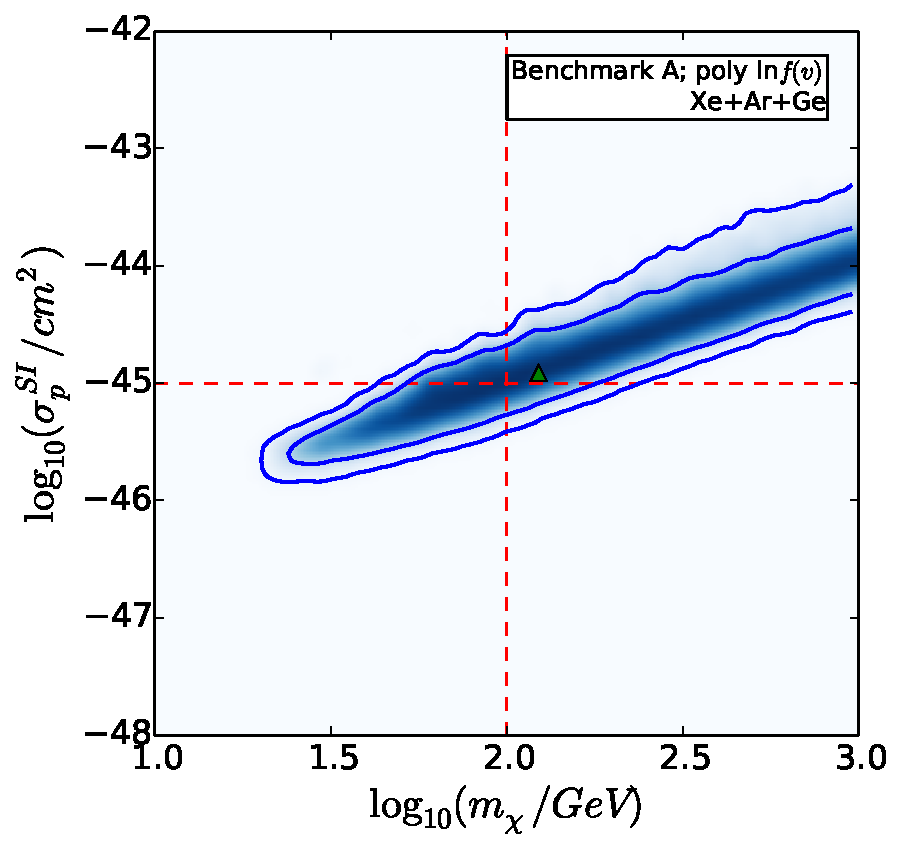
\includegraphics[width=0.32\textwidth]{NT/BenchmarkA_poly_noIC-mx_sigsi.pdf}
  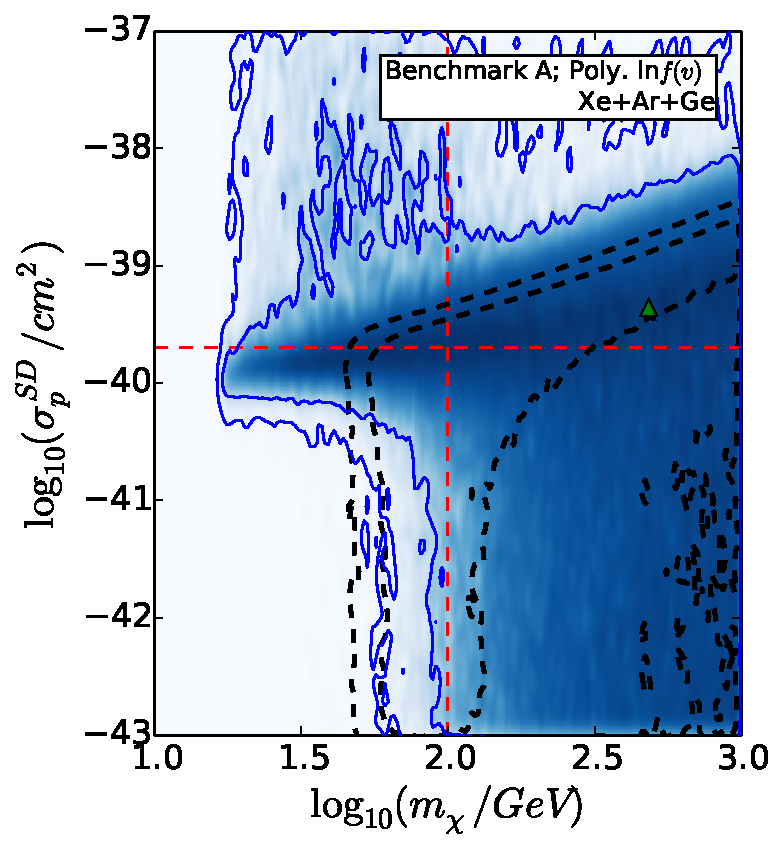
\includegraphics[width=0.32\textwidth]{NT/BenchmarkA_poly_noIC-mx_sigsd.pdf}
  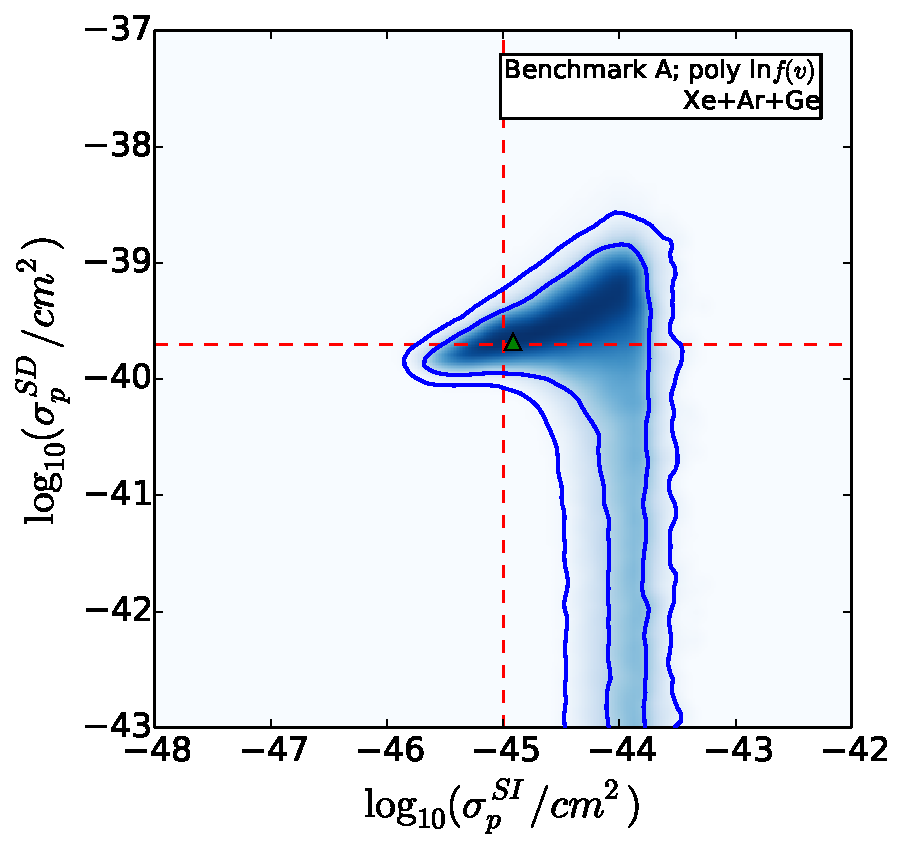
\includegraphics[width=0.32\textwidth]{NT/BenchmarkA_poly_noIC-sigsi_sigsd.pdf}

  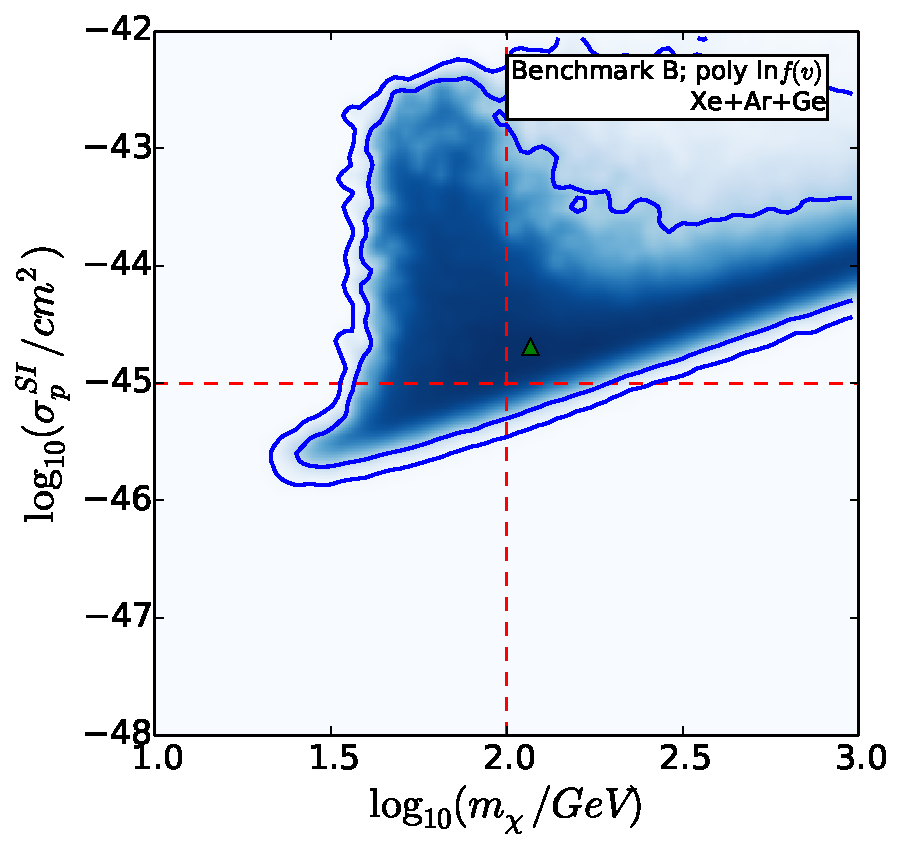
\includegraphics[width=0.32\textwidth]{NT/BenchmarkB_poly_noIC-mx_sigsi.pdf}
  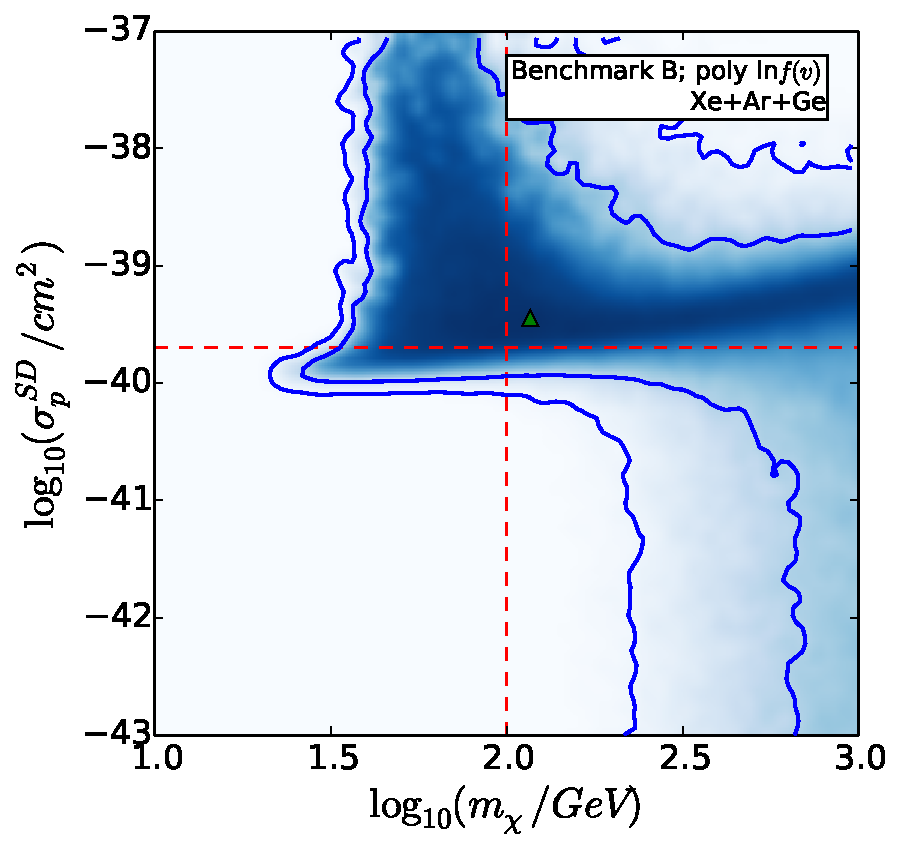
\includegraphics[width=0.32\textwidth]{NT/BenchmarkB_poly_noIC-mx_sigsd.pdf}
  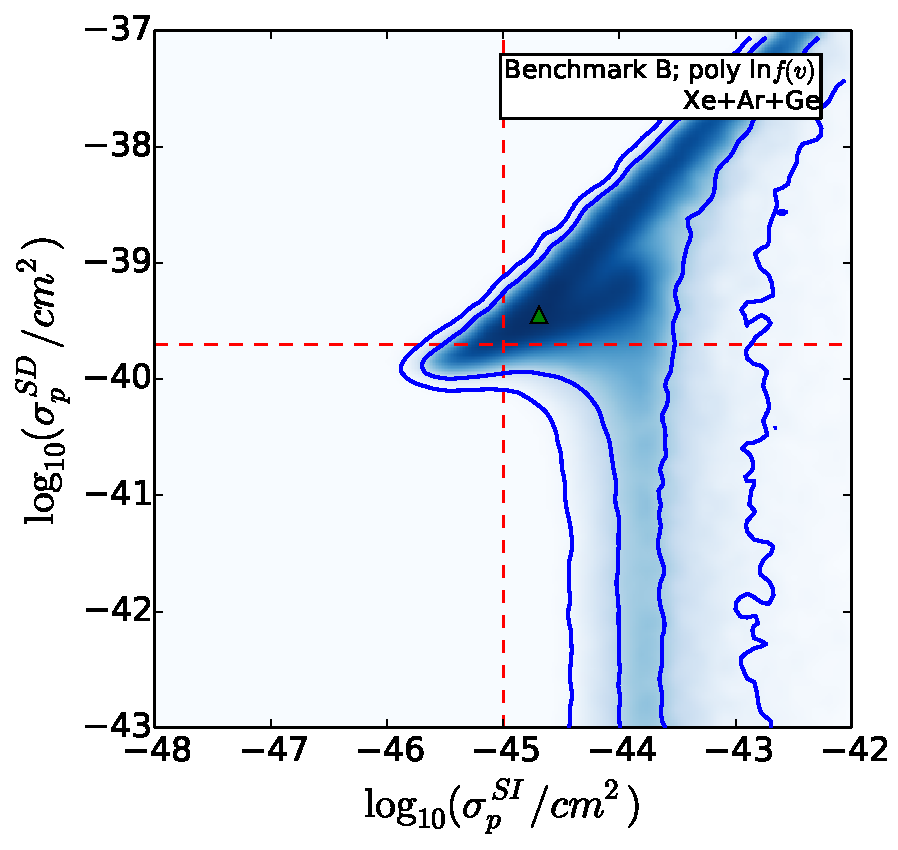
\includegraphics[width=0.32\textwidth]{NT/BenchmarkB_poly_noIC-sigsi_sigsd.pdf}

  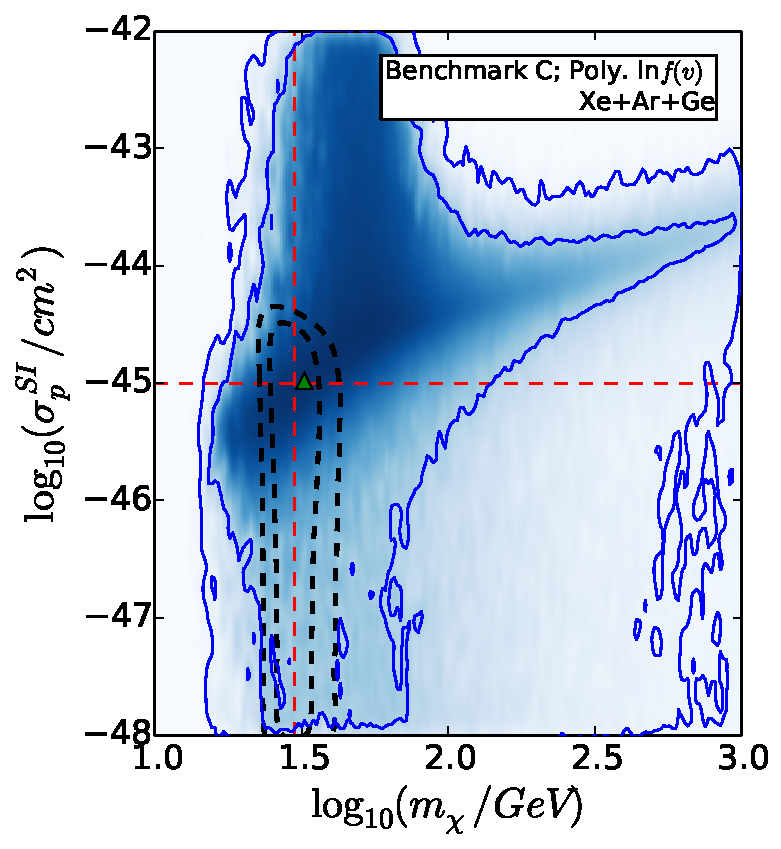
\includegraphics[width=0.32\textwidth]{NT/BenchmarkC_poly_noIC-mx_sigsi.pdf}
  \includegraphics[width=0.32\textwidth]{NT/BenchmarkC_poly_noIC-mx_sigsd.pdf}
  \includegraphics[width=0.32\textwidth]{NT/BenchmarkC_poly_noIC-sigsi_sigsd.pdf}

  \includegraphics[width=0.32\textwidth]{NT/BenchmarkD_poly_noIC-mx_sigsi.pdf}
  \includegraphics[width=0.32\textwidth]{NT/BenchmarkD_poly_noIC-mx_sigsd.pdf}
  \includegraphics[width=0.32\textwidth]{NT/BenchmarkD_poly_noIC-sigsi_sigsd.pdf}
\caption{WHAT!}
\end{figure}


\section{Reconstructions with IceCube}
\label{sec:NT:withIC}

\begin{figure}[!ht]
  \centering
  \includegraphics[width=0.32\textwidth]{NT/BenchmarkA_poly-mx_sigsi.pdf}
  \includegraphics[width=0.32\textwidth]{NT/BenchmarkA_poly-mx_sigsd.pdf}
  \includegraphics[width=0.32\textwidth]{NT/BenchmarkA_poly-sigsi_sigsd.pdf}

  \includegraphics[width=0.32\textwidth]{NT/BenchmarkB_poly-mx_sigsi.pdf}
  \includegraphics[width=0.32\textwidth]{NT/BenchmarkB_poly-mx_sigsd.pdf}
  \includegraphics[width=0.32\textwidth]{NT/BenchmarkB_poly-sigsi_sigsd.pdf}

  \includegraphics[width=0.32\textwidth]{NT/BenchmarkC_poly-mx_sigsi.pdf}
  \includegraphics[width=0.32\textwidth]{NT/BenchmarkC_poly-mx_sigsd.pdf}
  \includegraphics[width=0.32\textwidth]{NT/BenchmarkC_poly-sigsi_sigsd.pdf}

  \includegraphics[width=0.32\textwidth]{NT/BenchmarkD_poly-mx_sigsi.pdf}
  \includegraphics[width=0.32\textwidth]{NT/BenchmarkD_poly-mx_sigsd.pdf}
  \includegraphics[width=0.32\textwidth]{NT/BenchmarkD_poly-sigsi_sigsd.pdf}
\caption{WHAT!}
\end{figure}



\chapter{Speed parametrisation for directional experiments}

\section{Introduction}

While traditional direct detection experiments seek to measure the recoil energies deposited by WIMPs scattering off detector nuclei, \textit{directional} experiments aim to measure both the energy and direction of the recoil. While the recoil distribution of typical backgrounds is expected to be roughly isotropic, the WIMP-induced recoil distribution is expected to be highly directional. The motion of the Sun through the Galactic DM halo generates a so-called `WIMP wind,' leading to an event rate peaked in the opposing direction, the direction of the constellation of Cygnus. 

The ability of directional detection to distinguish background from signal and to provide a model independent confirmation of the dark matter origin of the signal make it a promising search strategy. However, measuring the direction of rare, low energy recoils remains challenging \cite{}. A number of directional detectors are currently in development and a number of novel methods for directional detection have been proposed.

Measuring the directional recoil spectrum allows us to probe not only the energy distribution of WIMPs in the Galactic halo (embodied in the speed distribution $f(v)$), but the full 3-dimensional velocity distribution $f(\textbf{v})$. This may allow us to gain new insight into the formation processes at hand in the growth of the Milky Way halo \cite{}. However, it also introduces new uncertainty into calculating the event rate. While non-directional detection leaves us with a single free function in the form of  $f(v)$, the directional case relies upon the \textit{a priori} unknown function of a 3-dimensional vector, $f(\textbf{v})$.

In this chapter, we will first introduce the formalism by which the directional rate is calculated. Specifically, we introduce the Radon transform which relates the WIMP velocity distribution to the corresponding nuclear recoil distribution.  We then discuss the current state of directional detection technology and the progress of several directional experiments. We then discuss previous approaches to mitigating the uncertainties associated with the velocity distribution. Finally, we consider a new method for parametrising $f(\textbf{v})$, which allows it to be written in terms of a finite number of one-dimensional functions, and how to calculate the Radon transform of this new, discretised distribution function.


\chapter{Conclusions}
\label{ch:Conclusions}

The presence of dark matter (DM) in the Universe has been postulated to explain a range of observations. Data from Cosmic Microwave Background anisotropies, the growth of large scale structure and the dynamics of galaxies and clusters all point towards a dark universe, with roughly 5 times as much dark matter as baryonic matter. So far, however, the detection of dark matter has only been through its gravitational influence. A number of experiments - so called direct detection experiments - are underway or in development which hope to detect weakly interacting massive particles (WIMPs) through their non-gravitational interactions in terrestrial detectors.

Once such a detection is confirmed, the next stage will be to try and measure the properties of the DM particles, such as their mass and interaction cross sections. This should help us to unravel the identity of the DM and begin to probe the structure of physics beyond the Standard Model of particle physics. However, the analysis of direct detection data is fraught with uncertainties. In this work, we have focused on astrophysical uncertainties, particularly those coming from the local speed distribution of dark matter $f_1(v)$. This distribution is \textit{a priori} unknown and a wide range of proposals having been put forward for its correct form. We cannot hope to accurately reconstruct the DM properties without first addressing these uncertainties.

Previous attempts to parametrise the DM speed distribution have been unsatisfactory. As we discuss in Chapter~\ref{ch:Speed}, these methods typically assume some specific functional form for the speed distribution, motivated by N-body simulations or assumptions of equilibrium. However, if the true shape of the speed distribution is poorly fit by the functional form assumed in the parametrisation, the particle physics parameters we are aiming to reconstruct will be biased. The aim then should be to develop a general, empirical parametrisation for the speed distribution which can be fit according to the data and which allows the DM mass and interaction cross sections to be reconstructed without bias. Such a parametrisation was first proposed by Peter \cite{Peter:2011}, in the form of a binned approximation to the speed distribution. However, this was shown to result in a bias in the reconstructed WIMP mass.

In Chapter~\ref{ch:Speed}, we demonstrated that this bias stems from the interplay between the WIMP mass and the size of the bins in energy. For a fixed bin width in speed, varying the WIMP mass affects not only the size of the corresponding bins in energy but also the number of bins to which an experiment is sensitive. The result is that the best fit to the data may not be provided by the true underlying WIMP mass.

This problem can be alleviated by using a binned parametrisation of the DM \textit{momentum} distribution. The range of momenta probed by a given experiment is independent of the WIMP mass, meaning that the overall shape and normalisation of the event spectrum can be probed separately. To pin down the WIMP mass, multiple experiments are required. In this case, the size and number of bins probed by each experiment depend only weakly on the WIMP mass, significantly reducing the bias seen in the binned speed parametrisation. We have also seen that the values of the momentum bin parameters may allow us to reconstruct the WIMP speed distribution itself. However, going from the reconstructed momentum distribution to the speed distribution is non-trivial. Moreover, the momentum binning method is expected to fail at low WIMP masses. Finally, this method requires a choice of the momentum range over which to parametrise, which may not always be obvious.

What properties then do we require of a general parametrisation of the WIMP distribution? It must be a physical distribution function, meaning that it must be everywhere non-negative and must be normalised. From our study of binned parametrisations, we are also lead to conclude that it should not have any fixed length scales, as these may result in a biased WIMP mass reconstruction. In light of this, we propose that the \textit{logarithm} of the directionally-averaged velocity distribution $f(v)$ should be written as a polynomial in the speed $v$ in the Earth frame. The resulting speed distribution takes the form
\begin{equation}
f_1(v) = v^2 \exp \left(\sum_{k=0}^{N-1} a_k P_k(v)\right)\,.
\end{equation}
This ensures that $f_1(v)$ is not only strictly positive, but also a smooth function of $v$. The shape of the speed distribution is controlled by the parameters $a_k$ and the $N$ basis functions $P_k$. Logarithmic dependence on the parameters also means that a wide range of functional forms can be approximated.

In Chapter \ref{ch:poly}, we have demonstrated that using this parametrisation the WIMP mass can be reconstructed without bias over a range of benchmark masses from 10 to 500 GeV. We have also demonstrated the method for a number of possible underlying distribution functions and shown that it has the correct statistical properties when Poisson fluctuations are included. We have also set out how best to choose the basis polynomials $P_k$ and the number of basis functions.

However, direct detection experiments have finite energy thresholds, which correspond to minimum WIMP speeds to which they are sensitive. Without information about the speed distribution below this threshold, it remains unconstrained by the experiments. This means that we do not know what fraction of WIMPs can contribute to scattering events in the detector. If we observe a small number of events at a detector, we cannot know whether they were caused by WIMPs with a low cross section or by WIMPs with a larger cross section but whose population is concentrated at low speeds. This results in a degeneracy between the cross section and the shape of the speed distribution. This degeneracy is a generic consequence of any general parametrisation of the WIMP speed distribution and means that we can only use direct detection experiments to place a lower bound on the interaction strengths of DM particles. As a consequence of this, we can only probe the \textit{shape} but not the normalisation of the WIMP speed distribution. In spite of this, it may still be possible to distinguish the Standard Halo Model from N-body speed distributions using around 1000 events.

In Chapter \ref{ch:NT}, we explore a method for breaking the speed distribution-cross section degeneracy. The capture of DM particles in the Sun is described by the same interaction cross sections which control the scattering rate in direct detection experiments. However, in the case of DM capture, it is those WIMPs with the lowest speeds which are more easily captured. Captured WIMPs then annihilate in the Sun and produce neutrinos, which can be detected at neutrino telescope experiments, such as IceCube. By combining future neutrino telescope and direct detection data, we can probe the entire range of the WIMP speed distribution. This allows us to constrain the fraction of low speed WIMPs and therefore break the degeneracy in the cross section, which we have demonstrated for several benchmarks.

We have also been able to reconstruct the WIMP speed distribution over the entire range of speeds. Maximum sensitivity is obtained at speeds close to the threshold speeds for the direct detection experiments, where the most spectral information is available. We have demonstrated that using next generation direct detection data, along with a signal from IceCube, it should be possible to detect evidence of a dark disk in the Milky Way at the $3\sigma$ level.


Finally, in Chapter \ref{ch:Directional}, we began to explore how such a parametrisation method could be extended to directional experiments. The signal at such experiments depends on the full 3-dimensional velocity distribution $f(\textbf{v})$. Parametrising such a function is unfeasible and would require a huge number of parameters. It is therefore necessary to decompose $f(\textbf{v})$ into a smaller number of basis functions. A spherical harmonic decomposition has been suggested previously. However, the spherical harmonic basis is not strictly positive, meaning that we cannot ensure that the velocity distribution is physical at every point in parameter space.

As an alternative, we propose an angular discretisation of the velocity distribution. As a first approximation, we have considered the forward- and backward-going distributions. However, with increasing amounts of data, it would be possible to increase the number of discretised pieces in $f(\textbf{v})$. This method allows us to constrain a small number of 1-dimensional functions $f^j(v)$, rather than a much larger space of 3-dimensional functions. We have laid out the framework for calculating the directional event rate from such a discrete parametrisation and have shown that with as few as $N=3$ discrete pieces, the event spectrum can be well fit by this approximation.

Further work is needed to understand how this discrete approximation behaves when confronted with mock data sets. In particular, we must combine this angular discretisation with the polynomial parametrisation we have developed for the speed distribution. This will allow us to determine how many discrete pieces are required for real data sets to ensure a close enough approximation to the true recoil spectrum. Though this method remains to be tested, we have established a framework which should allow the velocity distribution to be parametrised in a tractable way.

We have focused on astrophysical uncertainties in this work. However, many uncertainties remain in the analysis of direct detection data. Nuclear uncertainties associated with form factors and the spin and mass contributions of different quarks may also lead to biased inference if not properly accounted for. In addition, the standard contact interactions which lead to the spin-independent and spin-dependent scattering framework may not be correct. Higher order corrections or long-range interactions may have significant contributions to the scattering rate. It will be necessary in future to investigate the interplay between these different nuclear, particle and astrophysical uncertainties. In particular, understanding which combinations of experiments can best be used to disentangle these various uncertainties will allow us to extract the maximum information from future searches.

In this work, we have demonstrated for the first time that uncertainties in the WIMP speed distribution can be confronted and overcome in a completely general way. The polynomial $\ln f(v)$ parametrisation which we have proposed allows the WIMP mass to be reconstructed without bias, which we have demonstrated with a wide range of particle physics and astrophysics benchmarks. The introduction of neutrino telescope data allows us to probe the low speed population of WIMPs and therefore constrain not only the WIMP mass but also the WIMP interaction cross sections. We have also outlined how such a framework can be extended to incorporate directional data. This work is the first demonstration that both particle physics parameters \textit{and} the form of the speed distribution can be extracted from data from DM search experiments. It is hoped that these techniques will allow future direct detection experiments to not only reliably probe physics beyond the Standard Model, but also to be used as tools for WIMP astronomy.







%%%Problems with the style file: I've edited
%     pages empty$ {
%      doi output
%      } 'skip$ if$
%in the article FUNCTION to remove doi - it was adding it if other fields were missing, we don't want that...
%I've also removed some extra spaces which were messing with the hrefs...

\appendix
\chapter{Discretising the velocity distribution for arbitrary $N$}

\note{Check all of this and derive it too!!!}

We have to divide the range of $\beta$ into $N$ pieces. The sections are

\begin{align*}
\beta &\in \left[\cos\left(\frac{\pi}{2N}\right), 1\right]\,\\
\beta &\in \left[\cos\left(\frac{2\pi}{2N}\right), \cos\left(\frac{\pi}{2N}\right)\right]\,\\
& \vdots\\
\beta &\in \left[\cos\left(\frac{(N-1)\pi}{2N}\right), \cos\left(\frac{(N-2)\pi}{2N}\right)\right]\,\\
\beta &\in \left[0, \cos\left(\frac{(N-1)\pi}{2N}\right)\right]\,.\\
\end{align*}

We can label these by an index $n$, such that the limits are

\begin{equation}
\beta \in \left[\cos\left(\frac{n\pi}{2N}\right), \cos\left(\frac{(n-1)\pi}{2N}\right)\right]\,.
\end{equation}

\begin{comment}
\begin{align*}
\beta &\in \left[\cos\left(\frac{\pi}{N}\right), 1\right]\,\\
\beta &\in \left[\cos\left(\frac{2\pi}{N}\right), \cos\left(\frac{\pi}{N}\right)\right]\,\\
& \vdots\\
\beta &\in \left[\cos\left(\frac{(N-1)\pi}{N}\right), \cos\left(\frac{(N-2)\pi}{N}\right)\right]\,\\
\beta &\in \left[0, \cos\left(\frac{(N-1)\pi}{N}\right)\right]\,.\\
\end{align*}

We can label these by an index $n$, such that the limits are

\begin{align*}
\beta &\in \left[\cos\left(\frac{n\pi}{N}\right), \cos\left(\frac{(n-1)\pi}{N}\right)\right] \qquad \textrm{ for } n < l\,,\\
\beta &\in \left[0, \cos\left(\frac{l\pi}{N}\right)\right] \qquad \textrm{ for } n = l\,.
\end{align*}
\end{comment}
The limits of some of the integrals are

\begin{equation}
x_\pm = \beta \cos\theta \pm \sqrt{1-\beta^2}\sin\theta\,.
\end{equation}

The crossings of $x_+$ with the line $\cos\theta' = \cos(k\pi/N)$ are

\begin{align*}
\cos\theta &= \beta\cos(k\pi/N) + \sqrt{1-\beta^2}\sin(k\pi/N) & \textrm{ for } \beta < \cos(k\pi/N)\,,\\
\cos\theta &= \beta\cos(k\pi/N) - \sqrt{1-\beta^2}\sin(k\pi/N) & \textrm{ for } \beta > \cos((N-k)\pi/N)\,.\\
\end{align*}

Similarly for $x_-$, the crossing are at 

\begin{align*}
\cos\theta &= \beta\cos(k\pi/N) + \sqrt{1-\beta^2}\sin(k\pi/N) & \textrm{ for } \beta > \cos(k\pi/N)\,,\\
\cos\theta &= \beta\cos(k\pi/N) - \sqrt{1-\beta^2}\sin(k\pi/N) & \textrm{ for } \beta < \cos((N-k)\pi/N)\,.\\
\end{align*}

This partitions the range of $\cos\theta$ into $2N+1$ sections.

\note{I'm not sure how the above partitioning of $\beta$ is relevant...I'll check on the computer...Rewrite page 4 of the notes in terms of n which runs from 1 to 2N+1 (rather than just 1 to N) - that should make the m-1's simpler...}

\note{NB: have to be careful about the orderings of the end points...}

What are the edges of these $\cos\theta$ partitions?

\note{NB:$n$ should run from 1 to N}

\note{I may be missing some numerical factors...}

\note{I can probably simplify these expressions because for each $\hat{f}_j(v)$, there are only ever one or two bin contributions in $\cos\theta$...NOPE: there are exactly 3 bins for each...}

The edges of partition $m$ are:

%bin_edges[j] = np.cos(g - pi*(np.floor(n/2.0)+(0.5*(1+(-1)**(j+1))-np.floor((j+1)/2))*(-1)**(n+j))*1.0/N)

\begin{equation}
\left[A_{n,m}(\beta), A_{n,m-1}(\beta)\right]\,,
\end{equation}
where
\begin{equation}
A_{n,m}(\beta) = \cos\left(\acos{\beta} - \frac{\pi}{N}\left[\left \lfloor{\frac{n}{2}}\right \rfloor + \left(\frac{1}{2}(1 - (-1)^m) - \left \lfloor{\frac{m+1}{2}}\right \rfloor\right)(-1)^{n+m}\right]\right)\,.
\end{equation}

%plusvals = (np.floor(np.abs((n-m+0.5)/2)))+1
%minusvals = N-(np.floor(np.abs((n-(2*N+1 - m)-0.5)/2)))

\note{$m$ counts the number of crossings...}
When $\cos\theta$ falls in bin $m$, $x_+$ falls in bin:

\begin{equation}
k^{+}_{n,m} = \left \lfloor{\left|\frac{n-m+1/2}{2}\right|}\right \rfloor + 1\,,
\end{equation}
and $x_-$ falls in bin:
\begin{equation}
k^{-}_{n,m} = N - \left \lfloor{\left|\frac{n-(2N+1 -m)-1/2}{2}\right|}\right \rfloor\,.
\end{equation}

So for $\beta$ in range $n$ and $\cos\theta$ in bin $m$:

\begin{align*}
& \int_{-1}^{1} f(\textbf{v}) I(v_q, \cos\theta, \textbf{v}) \, \mathrm{d}\cos\theta'\\
&= \frac{2}{v} f_{k_{n,m}^+}(v) \left( \frac{\pi}{2} - \asin\left\{\frac{\cos(\pi k_{n,m}^{+}/N) - \beta \cos\theta}{\sqrt{1-\beta^2}\sin\theta}\right\}\right)\\
&+ \frac{2}{v} f_{k_{n,m}^-}(v) \left( \frac{\pi}{2} + \asin\left\{\frac{\cos(\pi (k_{n,m}^{-}-1)/N) - \beta \cos\theta}{\sqrt{1-\beta^2}\sin\theta}\right\}\right)\\
&+ \sum_{k = k_{n,m}^+ +1}^{k_{n,m}-1} \frac{2}{v} f_{k}(v) \left( \asin\left\{\frac{\cos(\pi (k-1)/N) - \beta \cos\theta}{\sqrt{1-\beta^2}\sin\theta}\right\}\right. \\
&\qquad\qquad\qquad\qquad- \left.\asin\left\{\frac{\cos(\pi (k)/N) - \beta \cos\theta}{\sqrt{1-\beta^2}\sin\theta}\right\}\right)\,.
\end{align*}

We write the integral:
\begin{equation}
\int \asin\left\{\frac{y - \beta \cos\theta}{\sqrt{1-\beta^2}\sin\theta}\right\} \, \mathrm{d}\cos\theta \equiv J(\cos\theta; y) + C\,,
\end{equation}
where it is understood that $J$ depends implicityly on $\beta$. 

For $\beta$ in range $n$, we want to integrate over $\cos\theta \in [\cos(\pi j/N), \cos(\pi (j-1)/N)]$. There are only three `bins' in $\cos\theta$ which contribute:

\begin{align*}
\cos\theta \in & [\cos(\pi j/N), A_{n,2(j-1)+1}(\beta)]\,, \\
\cos\theta \in & [A_{n,2(j-1)+1}(\beta), A_{n,2(j-1)+2}(\beta)]\,, \\
\cos\theta \in & [A_{n,2(j-1)+2}(\beta), \cos(\pi (j-1)/N)]\,,
\end{align*}
We write these 4 edges as $B_{n, i}$ where $i = 1,2,3,4$. Integrating then over the range $\cos\theta \in [B_{n,i}, B_{n,i+1}]$ and summing, we obtain:

\begin{align*}
& \sum_{i = 1,3}\int_{B_{n,i}}^{B_{n,i+1}} \int_{-1}^{1} f(\textbf{v}) I(v_q, \cos\theta, \textbf{v}) \, \mathrm{d}\cos\theta' \, \mathrm{d}\cos\theta\\
&=\sum_{i = 1,3} \frac{2}{v} f_{k_{n,2(j-1)+i}^+}(v) \left( \frac{\pi}{2}(B_{n,i+1} - B_{n,i}) \right.\\
&\qquad\qquad - \left.J(B_{n,i+1}; \cos(\pi k_{n,2(j-1)+i}^{+}/N)) + J(B_{n,i}; \cos(\pi k_{n,2(j-1)+i}^{+}/N))\right)\\
&+ \frac{2}{v} f_{k_{n,2(j-1)+i}^-}(v) \left( \frac{\pi}{2}(B_{n,i+1} - B_{n,i})\right. \\
&\qquad\qquad + \left. J(B_{n,i+1}; \cos(\pi (k_{n,2(j-1)+i}^{-}-1)/N)) - J(B_{n,i}; \cos(\pi (k_{n,2(j-1)+i}^{-}-1)/N))\right)\\
&+ \sum_{k = k_{n,2(j-1)+i}^+ +1}^{k_{n,2(j-1)+i}-1} \frac{2}{v} f_{k}(v) \left( J(B_{n,i+1};\cos(\pi (k-1)/N)) - J(B_{n,i};\cos(\pi (k-1)/N))\right. \\
&\qquad\qquad - \left. J(B_{n,i+1};\cos(\pi (k)/N)) + J(B_{n,i};\cos(\pi (k)/N)) \right)\\
&\equiv \sum_{i=1,2,3} \Gamma_{n,j,i}(v)\,.
\end{align*}

\note{NB:Check numerical factors...}
Finally, we have to integrate over $v$ or, equivalently, $\beta$:

\begin{equation}
\hat{f}_j(v) = \sum_{n = 1,N} \sum_{i=1,2,3} \int_{v_q/\cos((n-1)\pi/(2N))}^{v_q/\cos(n\pi/(2N))}  \Gamma_{n,j,i}(v) \, \mathrm{d}v\,,
\end{equation}
where the $\Gamma_{n,j,i}$ depend on $j$ through the values of $B_{n,i}$ and the indices of $f_k$.

\note{I can always refer back to the code to check - because the code gives the right values of things...}


\bibliographystyle{my-apsrev4-2}
\bibliography{Thesis,Experiments,DMDensity}

\end{document}
